%
\subsection{Analysis Regions}
\begin{figure}[htbp!]
    \begin{subfigure}[t]{1\textwidth}
    \begin{center}
    
\includegraphics[width=0.4\textwidth]{figures/NNPlots/analysisRegion/NoRew/ljets_8j3bL.pdf}
    
\includegraphics[width=0.4\textwidth]{figures/NNPlots/analysisRegion/Rew/ljets_8j3bL.pdf}
    \caption{8j3bL}
    \end{center}
    \end{subfigure}

    \begin{subfigure}[t]{1\textwidth}
    \begin{center}
    
\includegraphics[width=0.4\textwidth]{figures/NNPlots/analysisRegion/NoRew/ljets_8j3bH.pdf}
    
\includegraphics[width=0.4\textwidth]{figures/NNPlots/analysisRegion/Rew/ljets_8j3bH.pdf}
    \caption{8j3bH}
    \end{center}
    \end{subfigure}

    \begin{subfigure}[t]{1\textwidth}
    \begin{center}
    
\includegraphics[width=0.4\textwidth]{figures/NNPlots/analysisRegion/NoRew/ljets_8j4b.pdf}
    
\includegraphics[width=0.4\textwidth]{figures/NNPlots/analysisRegion/Rew/ljets_8j4b.pdf}
    \caption{8j4b}
    \end{center}
    \end{subfigure}
    \caption{\label{fig:NNPlots_AnaReg_1} The comparison between variables distribution before (left) and after (right) the NN-reweighting in 1L 8j regions.}  
\end{figure}

\begin{figure}[htbp!]
    \begin{subfigure}[t]{1\textwidth}
    \begin{center}
    
\includegraphics[width=0.4\textwidth]{figures/NNPlots/analysisRegion/NoRew/ljets_9j3bL.pdf}
    
\includegraphics[width=0.4\textwidth]{figures/NNPlots/analysisRegion/Rew/ljets_9j3bL.pdf}
    \caption{9j3bL}
    \end{center}
    \end{subfigure}

    \begin{subfigure}[t]{1\textwidth}
    \begin{center}
    
\includegraphics[width=0.4\textwidth]{figures/NNPlots/analysisRegion/NoRew/ljets_9j3bH.pdf}
    
\includegraphics[width=0.4\textwidth]{figures/NNPlots/analysisRegion/Rew/ljets_9j3bH.pdf}
    \caption{9j3bH}
    \end{center}
    \end{subfigure}

    \begin{subfigure}[t]{1\textwidth}
    \begin{center}
    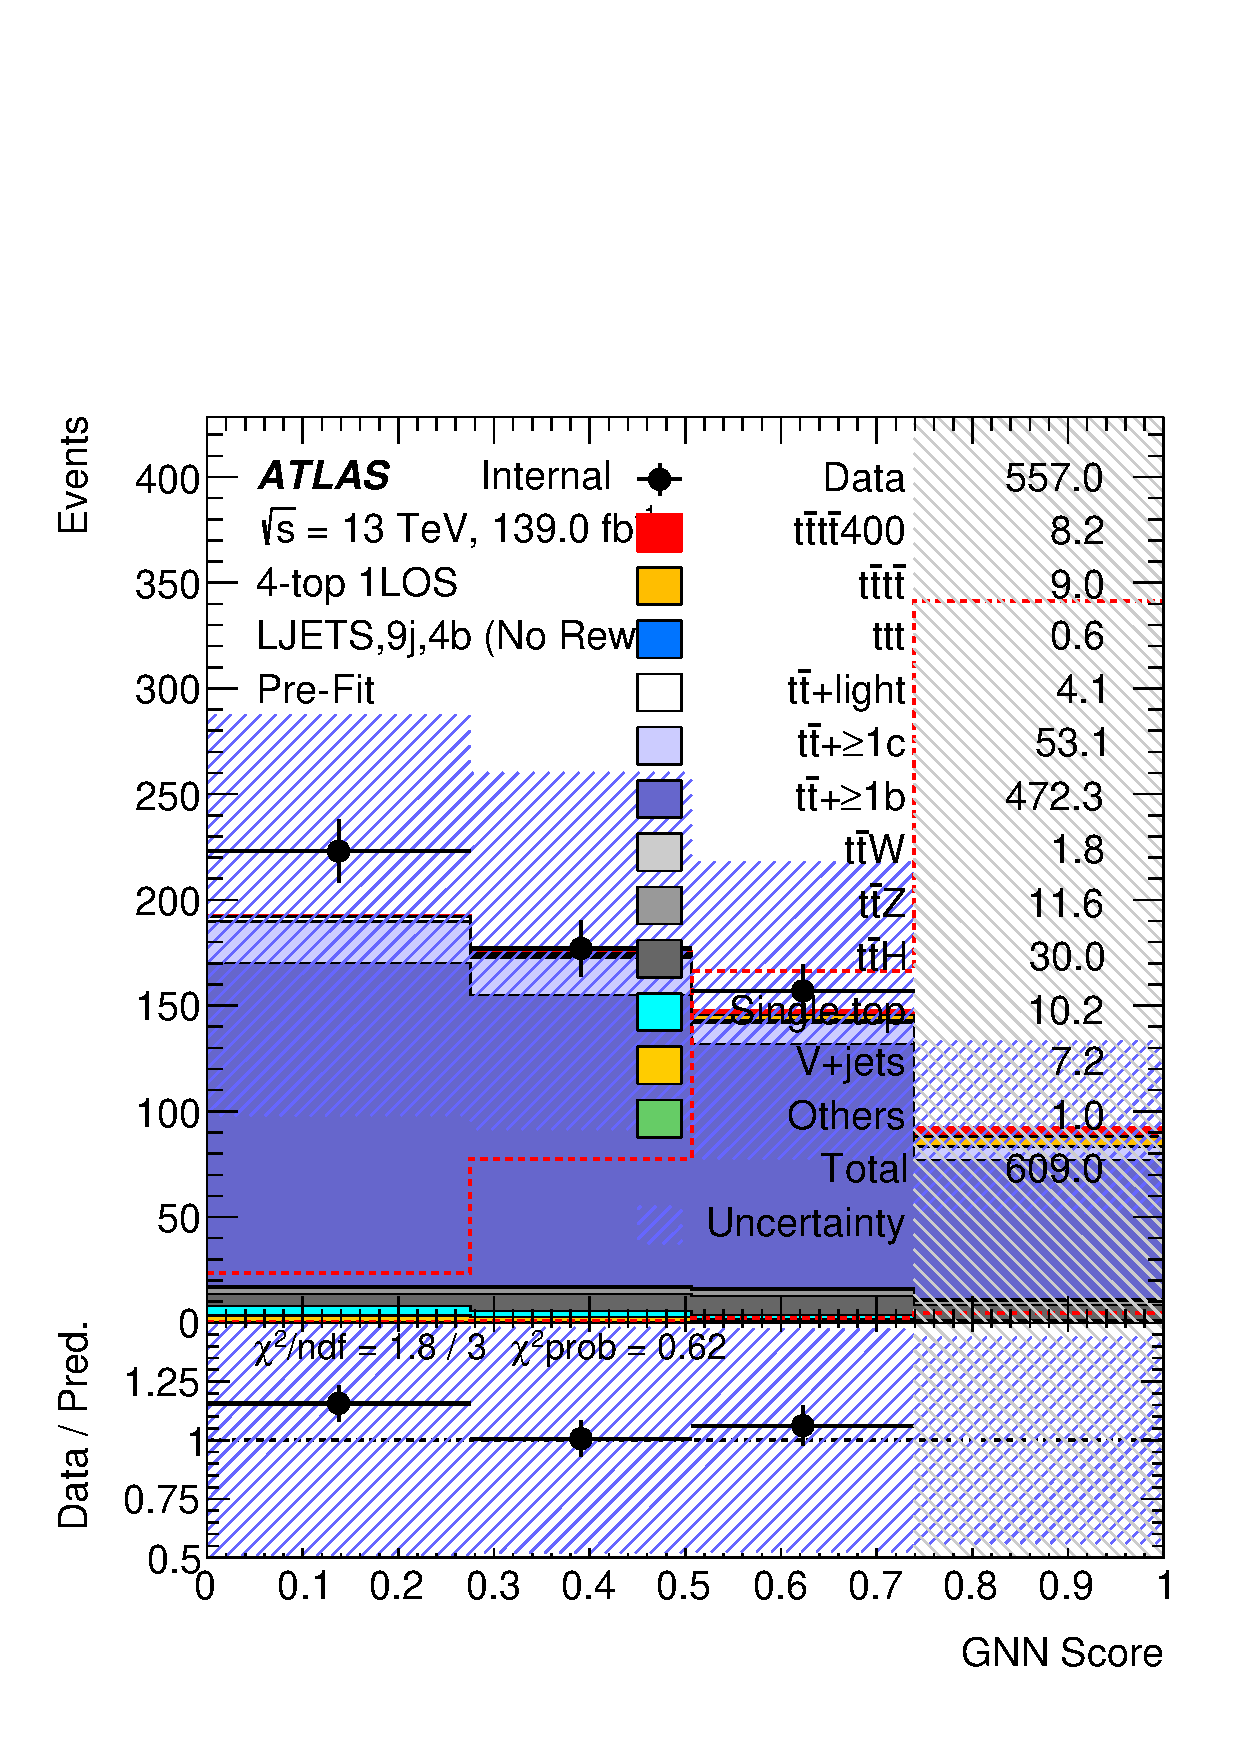
\includegraphics[width=0.4\textwidth]{figures/NNPlots/analysisRegion/NoRew/ljets_9j4b_SR.pdf}
    
\includegraphics[width=0.4\textwidth]{figures/NNPlots/analysisRegion/Rew/ljets_9j4b_SR.pdf}
    \caption{9j4b}
    \end{center}
    \end{subfigure}
    \caption{\label{fig:NNPlots_AnaReg_2} The comparison between variables distribution before (left) and after (right) the NN-reweighting in 1L 9j regions.}  
\end{figure}

\begin{figure}[htbp!]
    \begin{subfigure}[t]{1\textwidth}
    \begin{center}
    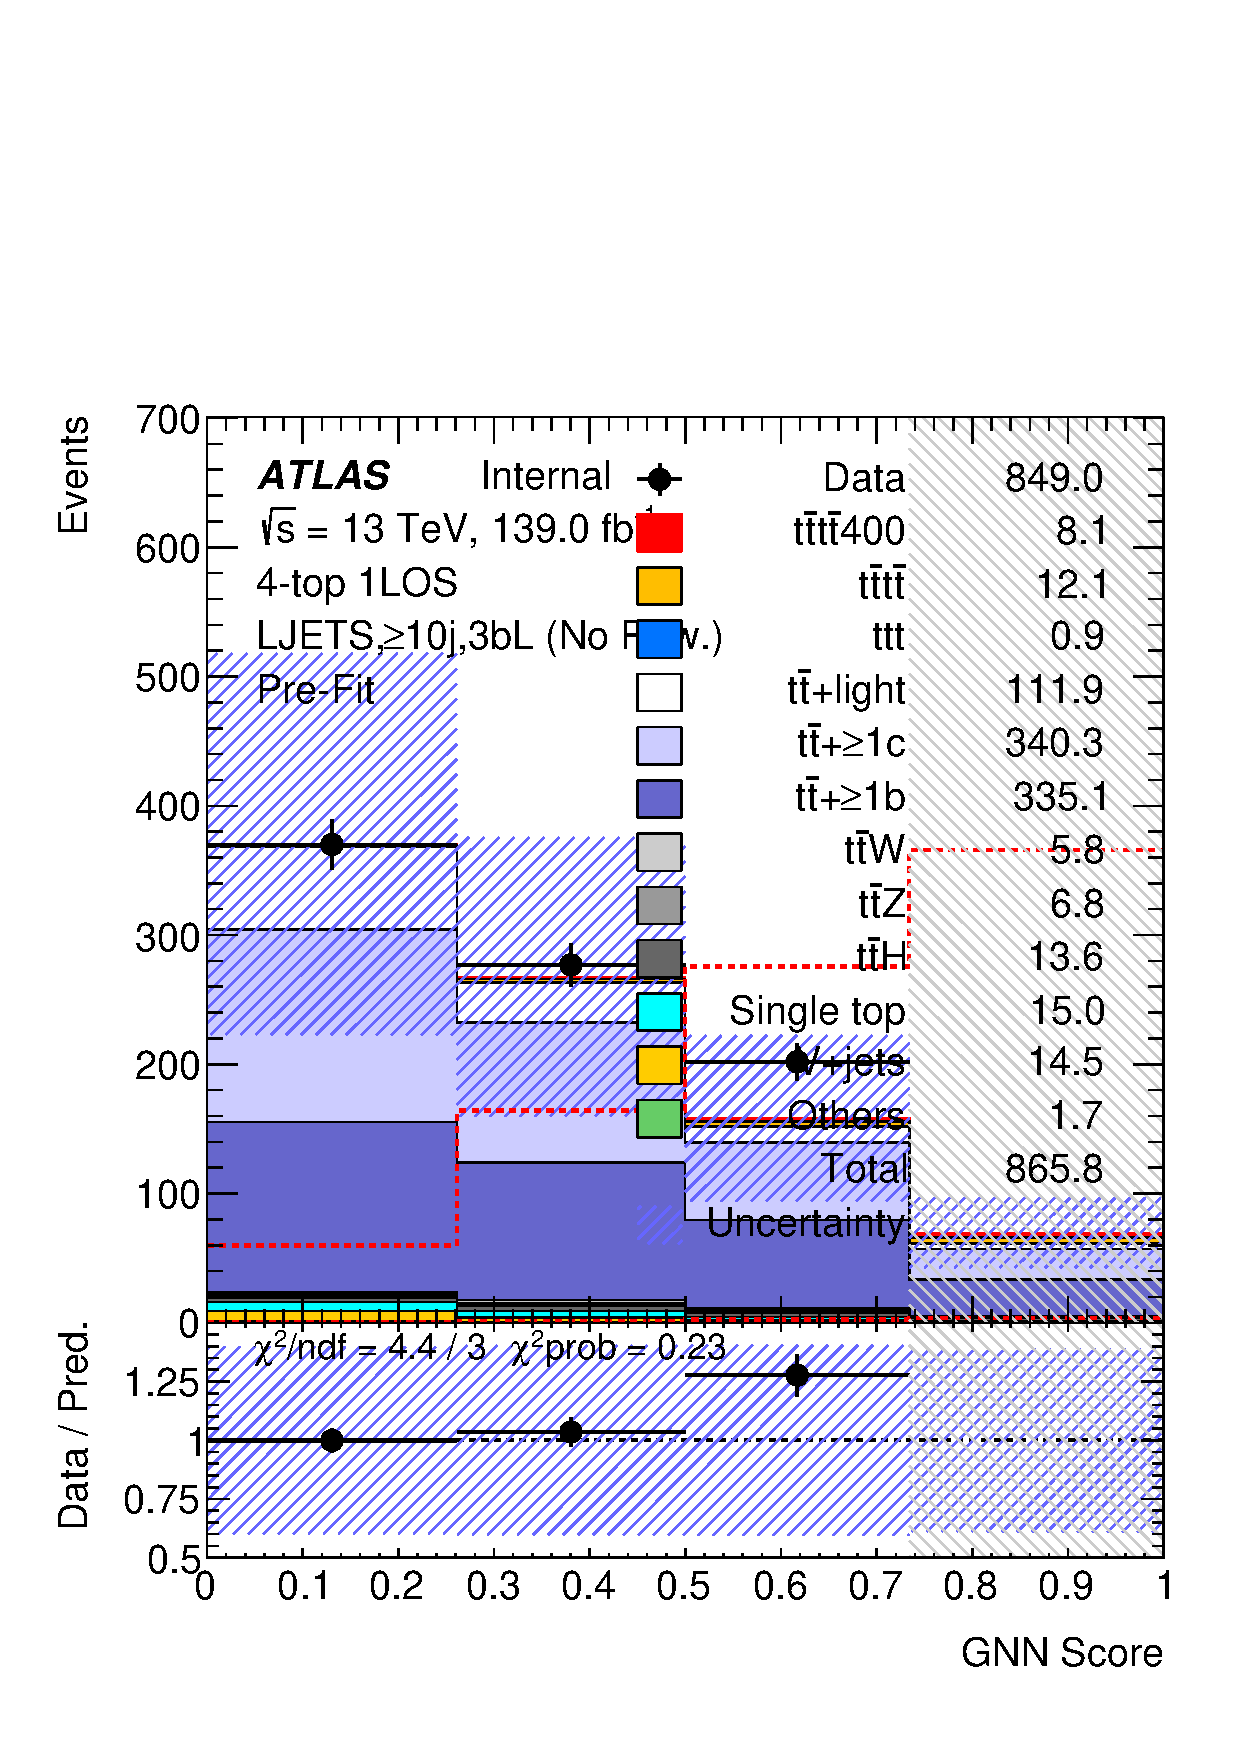
\includegraphics[width=0.4\textwidth]{figures/NNPlots/analysisRegion/NoRew/ljets_ge10j3bL_SR.pdf}
    
\includegraphics[width=0.4\textwidth]{figures/NNPlots/analysisRegion/Rew/ljets_ge10j3bL_SR.pdf}
    \caption{ge10j3bL}
    \end{center}
    \end{subfigure}

    \begin{subfigure}[t]{1\textwidth}
    \begin{center}
    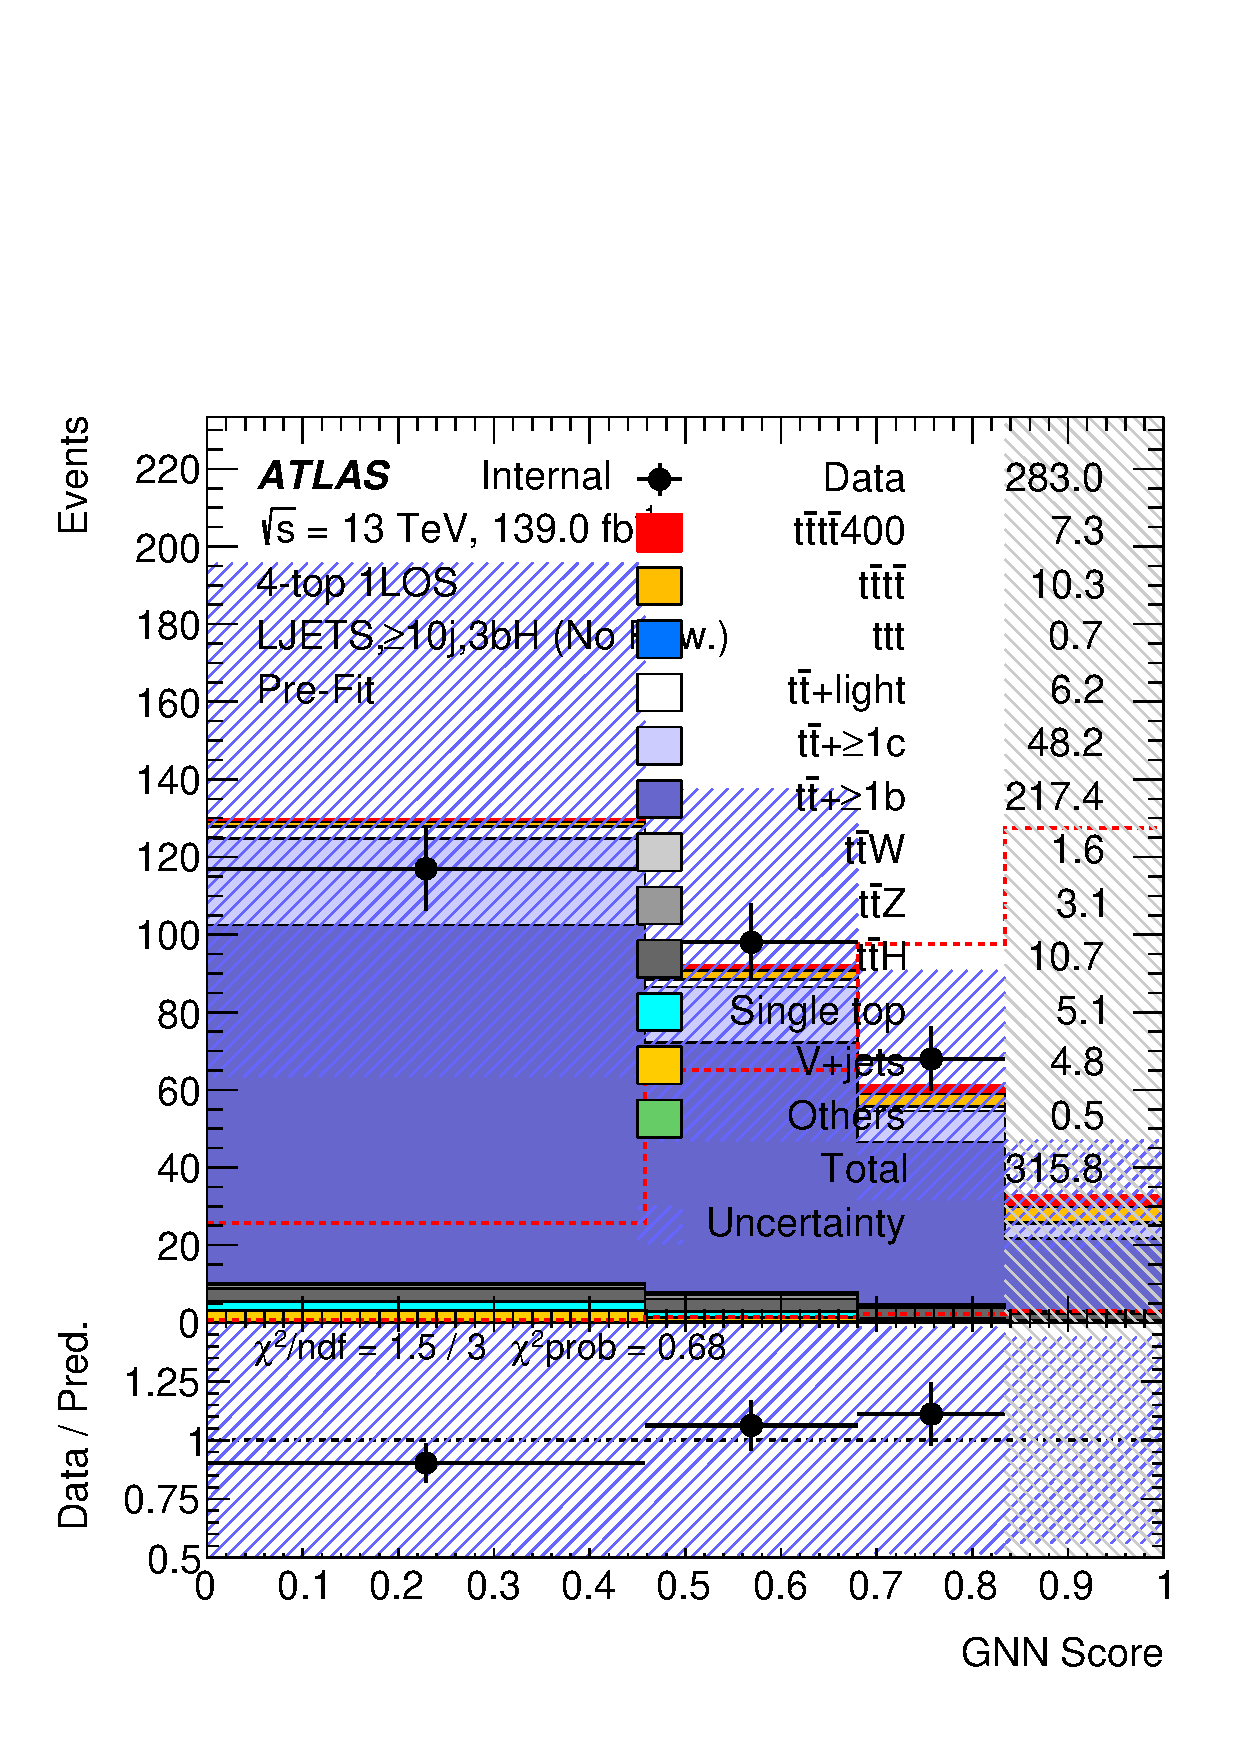
\includegraphics[width=0.4\textwidth]{figures/NNPlots/analysisRegion/NoRew/ljets_ge10j3bH_SR.pdf}
    
\includegraphics[width=0.4\textwidth]{figures/NNPlots/analysisRegion/Rew/ljets_ge10j3bH_SR.pdf}
    \caption{ge10j3bH}
    \end{center}
    \end{subfigure}

    \begin{subfigure}[t]{1\textwidth}
    \begin{center}
    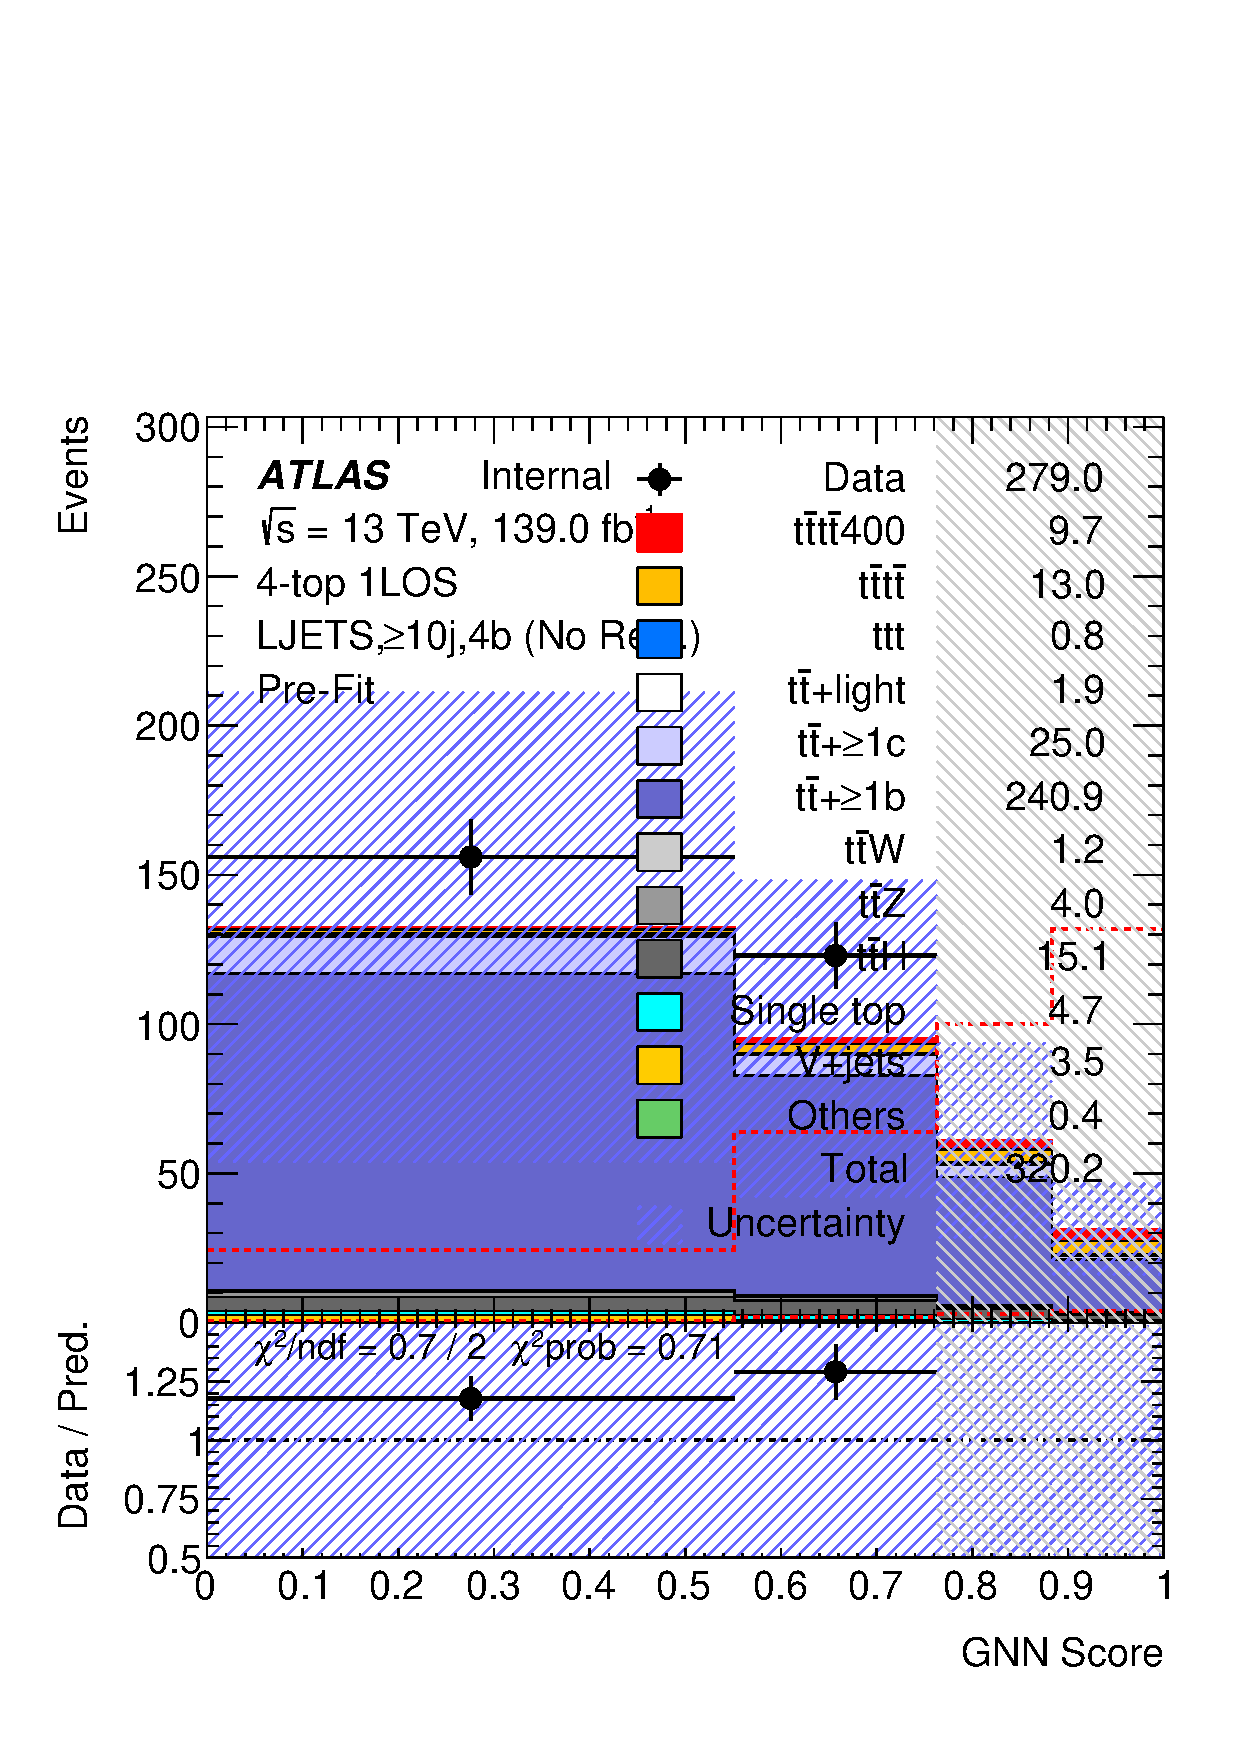
\includegraphics[width=0.4\textwidth]{figures/NNPlots/analysisRegion/NoRew/ljets_ge10j4b_SR.pdf}
    
\includegraphics[width=0.4\textwidth]{figures/NNPlots/analysisRegion/Rew/ljets_ge10j4b_SR.pdf}
    \caption{ge10j4b}
    \end{center}
    \end{subfigure}
    \caption{\label{fig:NNPlots_AnaReg_3} The comparison between variables distribution before (left) and after (right) the NN-reweighting in 1L $\geq 10j$ regions.}  
\end{figure}

\begin{figure}[htbp!]
    \begin{subfigure}[t]{1\textwidth}
    \begin{center}
    
\includegraphics[width=0.4\textwidth]{figures/NNPlots/analysisRegion/NoRew/os2l_6j3bL.pdf}
    
\includegraphics[width=0.4\textwidth]{figures/NNPlots/analysisRegion/Rew/os2l_6j3bL.pdf}
    \caption{6j3bL}
    \end{center}
    \end{subfigure}

    \begin{subfigure}[t]{1\textwidth}
    \begin{center}
    
\includegraphics[width=0.4\textwidth]{figures/NNPlots/analysisRegion/NoRew/os2l_6j3bH.pdf}
    
\includegraphics[width=0.4\textwidth]{figures/NNPlots/analysisRegion/Rew/os2l_6j3bH.pdf}
    \caption{6j3bH}
    \end{center}
    \end{subfigure}

    \begin{subfigure}[t]{1\textwidth}
    \begin{center}
    
\includegraphics[width=0.4\textwidth]{figures/NNPlots/analysisRegion/NoRew/os2l_6jge4b.pdf}
    
\includegraphics[width=0.4\textwidth]{figures/NNPlots/analysisRegion/Rew/os2l_6jge4b.pdf}
    \caption{6jge4b}
    \end{center}
    \end{subfigure}
    \caption{\label{fig:NNPlots_AnaReg_4} The comparison between variables distribution before (left) and after (right) the NN-reweighting in 2LOS 6j regions.}  
\end{figure}

\begin{figure}[htbp!]
    \begin{subfigure}[t]{1\textwidth}
    \begin{center}
    
\includegraphics[width=0.4\textwidth]{figures/NNPlots/analysisRegion/NoRew/os2l_6j3bL.pdf}
    
\includegraphics[width=0.4\textwidth]{figures/NNPlots/analysisRegion/Rew/os2l_6j3bL.pdf}
    \caption{6j3bL}
    \end{center}
    \end{subfigure}

    \begin{subfigure}[t]{1\textwidth}
    \begin{center}
    
\includegraphics[width=0.4\textwidth]{figures/NNPlots/analysisRegion/NoRew/os2l_6j3bH.pdf}
    
\includegraphics[width=0.4\textwidth]{figures/NNPlots/analysisRegion/Rew/os2l_6j3bH.pdf}
    \caption{6j3bH}
    \end{center}
    \end{subfigure}

    \begin{subfigure}[t]{1\textwidth}
    \begin{center}
    
\includegraphics[width=0.4\textwidth]{figures/NNPlots/analysisRegion/NoRew/os2l_6jge4b.pdf}
    
\includegraphics[width=0.4\textwidth]{figures/NNPlots/analysisRegion/Rew/os2l_6jge4b.pdf}
    \caption{6jge4b}
    \end{center}
    \end{subfigure}
    \caption{\label{fig:NNPlots_AnaReg_5} The comparison between variables distribution before (left) and after (right) the NN-reweighting in 2LOS 6j regions.}  
\end{figure}

\begin{figure}[htbp!]
    \begin{subfigure}[t]{1\textwidth}
    \begin{center}
    
\includegraphics[width=0.4\textwidth]{figures/NNPlots/analysisRegion/NoRew/os2l_7j3bL.pdf}
    
\includegraphics[width=0.4\textwidth]{figures/NNPlots/analysisRegion/Rew/os2l_7j3bL.pdf}
    \caption{7j3bL}
    \end{center}
    \end{subfigure}

    \begin{subfigure}[t]{1\textwidth}
    \begin{center}
    
\includegraphics[width=0.4\textwidth]{figures/NNPlots/analysisRegion/NoRew/os2l_7j3bH.pdf}
    
\includegraphics[width=0.4\textwidth]{figures/NNPlots/analysisRegion/Rew/os2l_7j3bH.pdf}
    \caption{7j3bH}
    \end{center}
    \end{subfigure}

    \begin{subfigure}[t]{1\textwidth}
    \begin{center}
    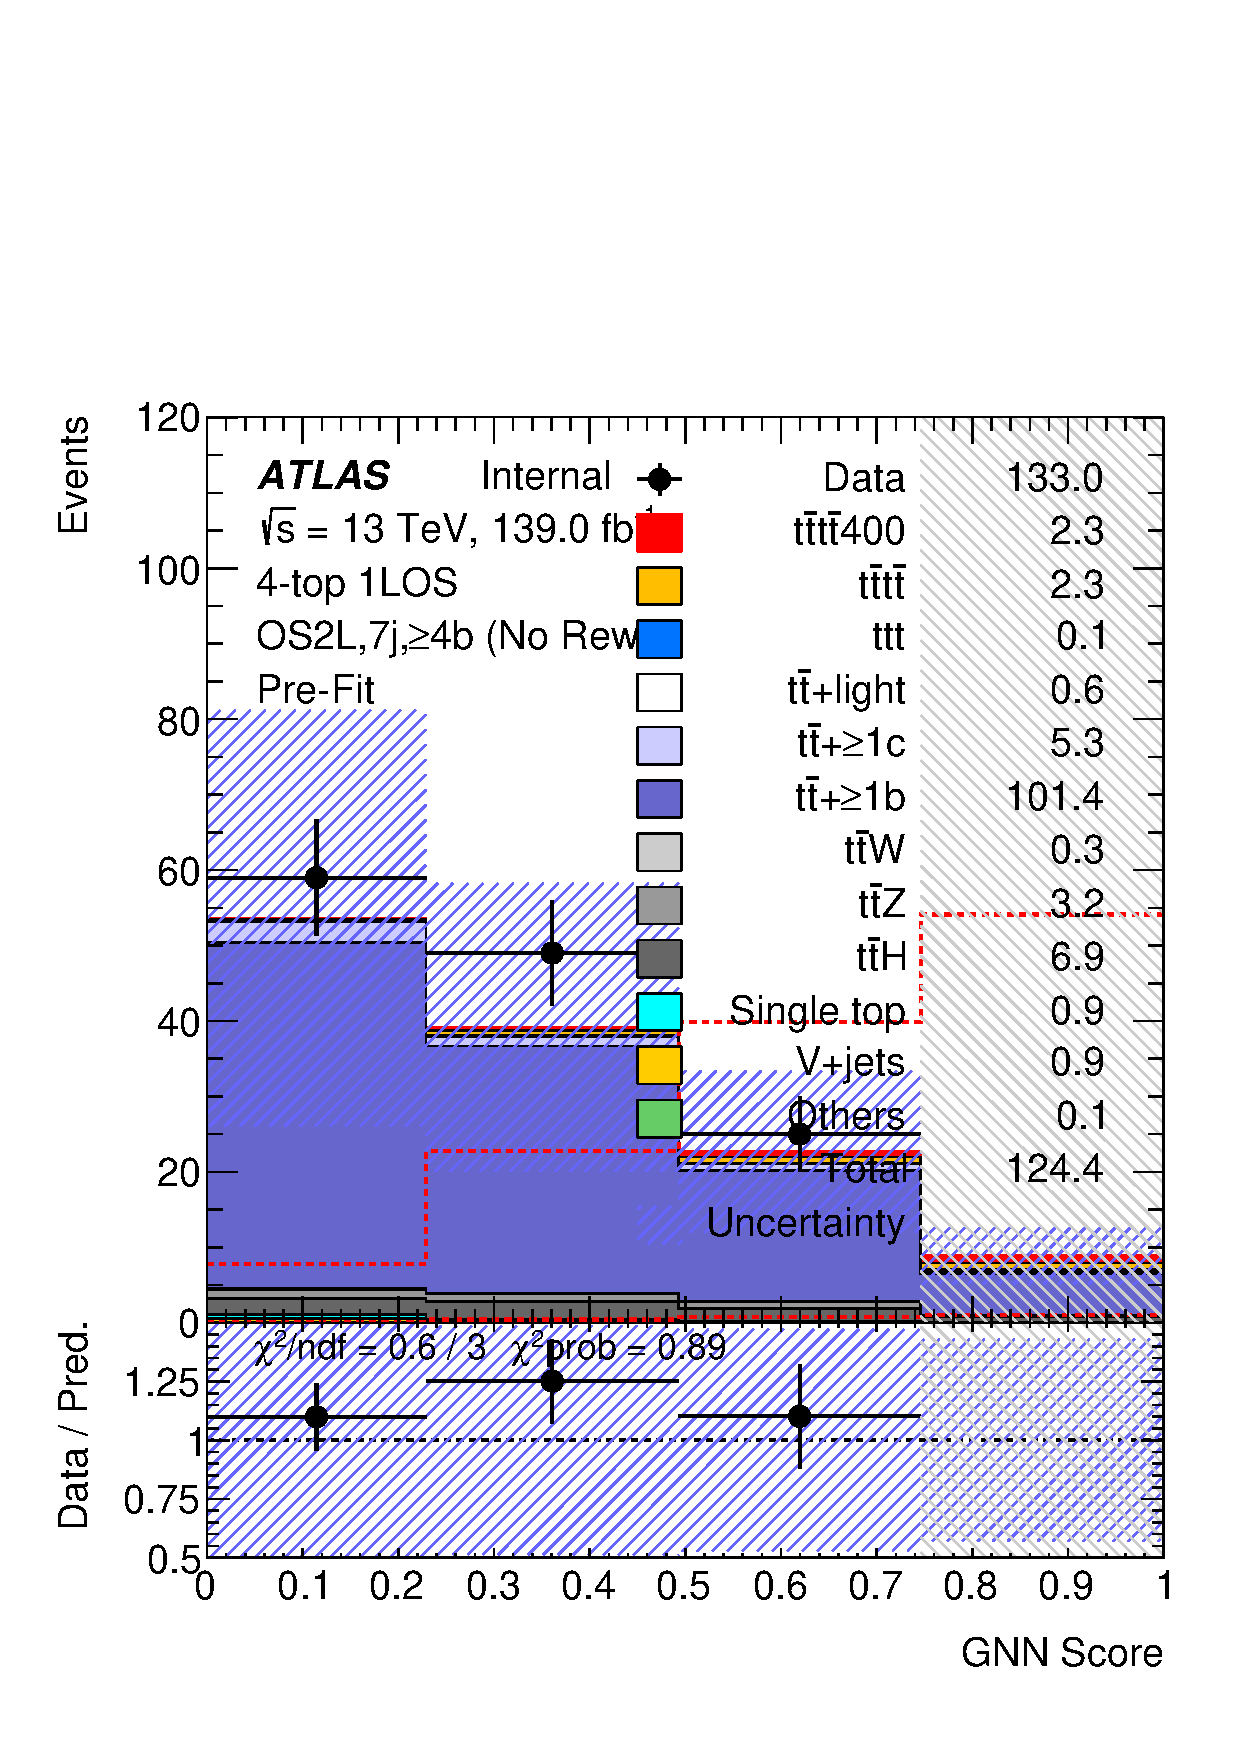
\includegraphics[width=0.4\textwidth]{figures/NNPlots/analysisRegion/NoRew/os2l_7jge4b_SR.pdf}
    
\includegraphics[width=0.4\textwidth]{figures/NNPlots/analysisRegion/Rew/os2l_7jge4b_SR.pdf}
    \caption{7jge4b}
    \end{center}
    \end{subfigure}
    \caption{\label{fig:NNPlots_AnaReg_5} The comparison between variables distribution before (left) and after (right) the NN-reweighting in 2LOS 7j regions.}  
\end{figure}

\begin{figure}[htbp!]
    \begin{subfigure}[t]{1\textwidth}
    \begin{center}
    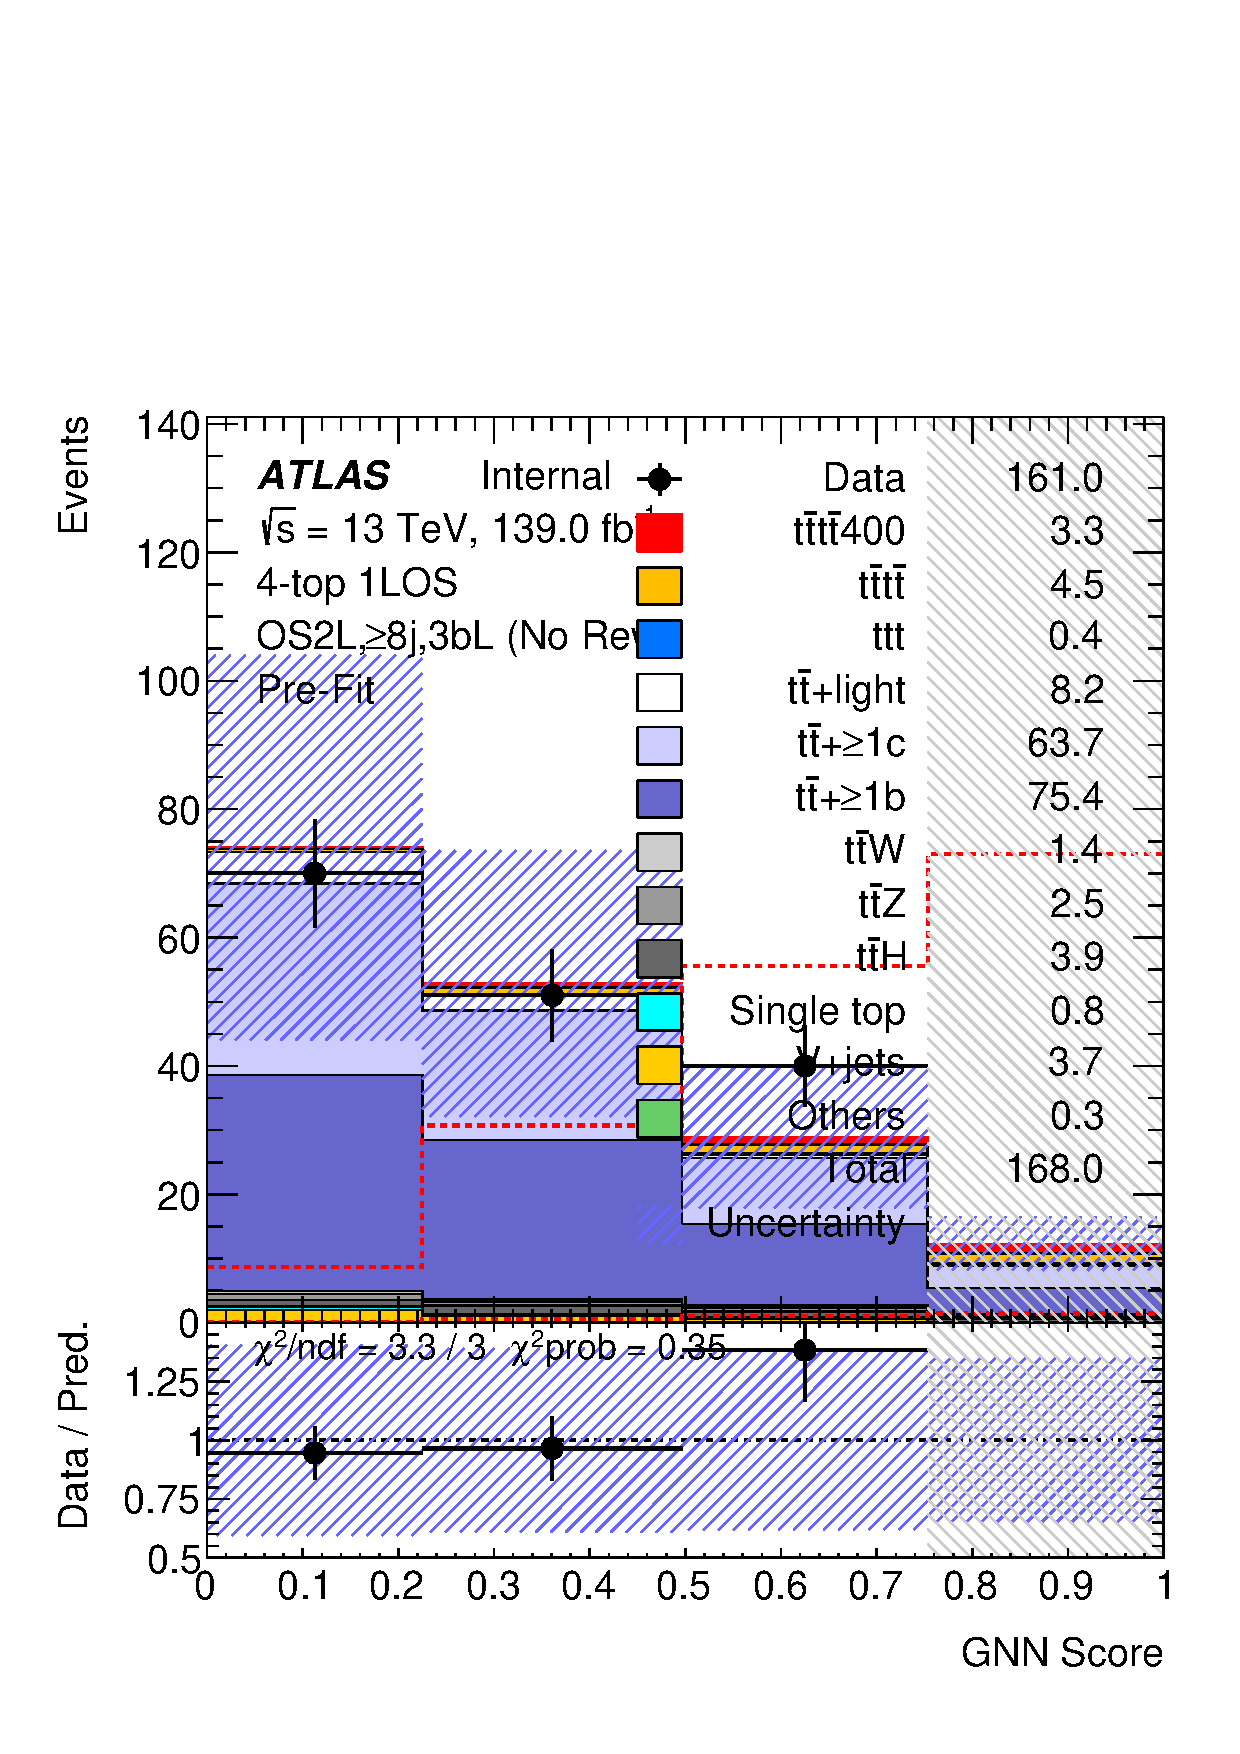
\includegraphics[width=0.4\textwidth]{figures/NNPlots/analysisRegion/NoRew/os2l_ge8j3bL_SR.pdf}
    
\includegraphics[width=0.4\textwidth]{figures/NNPlots/analysisRegion/Rew/os2l_ge8j3bL_SR.pdf}
    \caption{ge8j3bL}
    \end{center}
    \end{subfigure}

    \begin{subfigure}[t]{1\textwidth}
    \begin{center}
    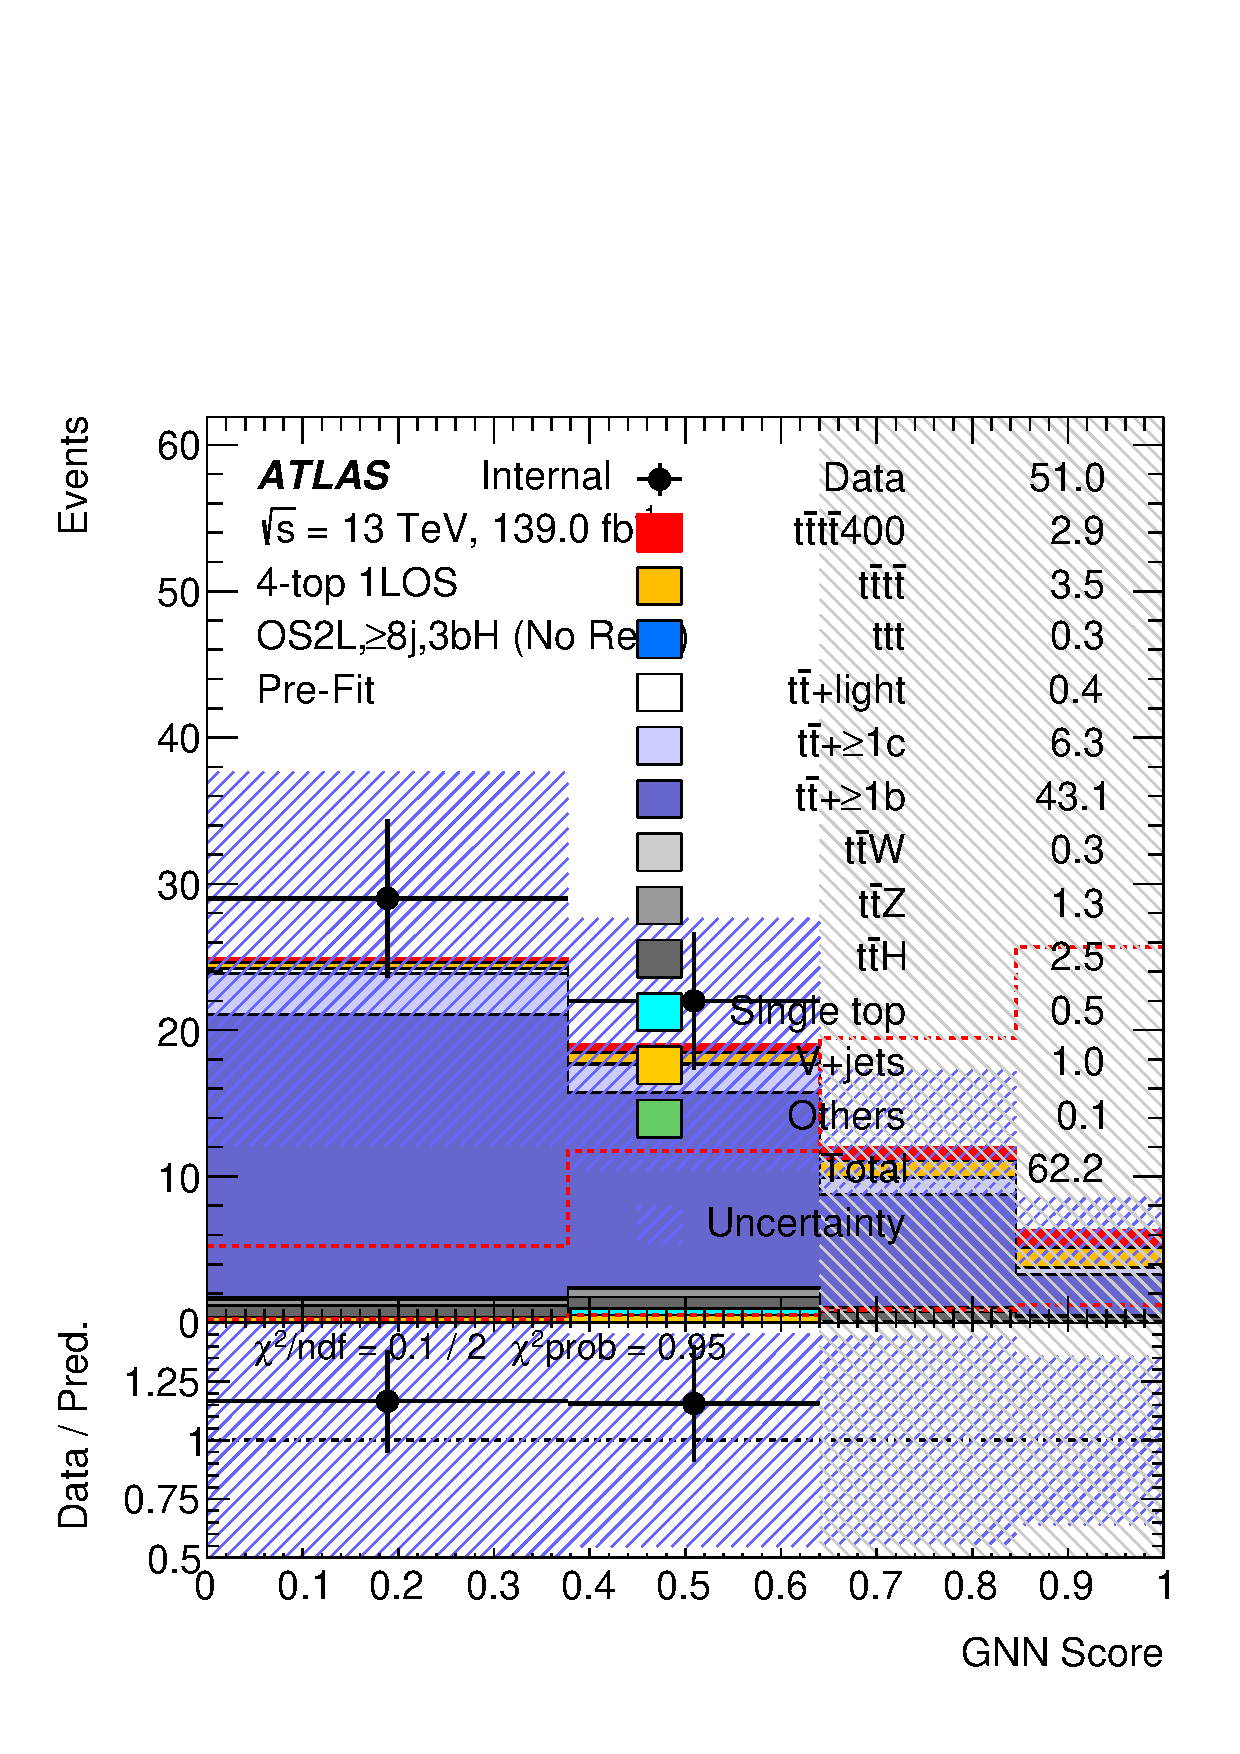
\includegraphics[width=0.4\textwidth]{figures/NNPlots/analysisRegion/NoRew/os2l_ge8j3bH_SR.pdf}
    
\includegraphics[width=0.4\textwidth]{figures/NNPlots/analysisRegion/Rew/os2l_ge8j3bH_SR.pdf}
    \caption{ge8j3bH}
    \end{center}
    \end{subfigure}

    \begin{subfigure}[t]{1\textwidth}
    \begin{center}
    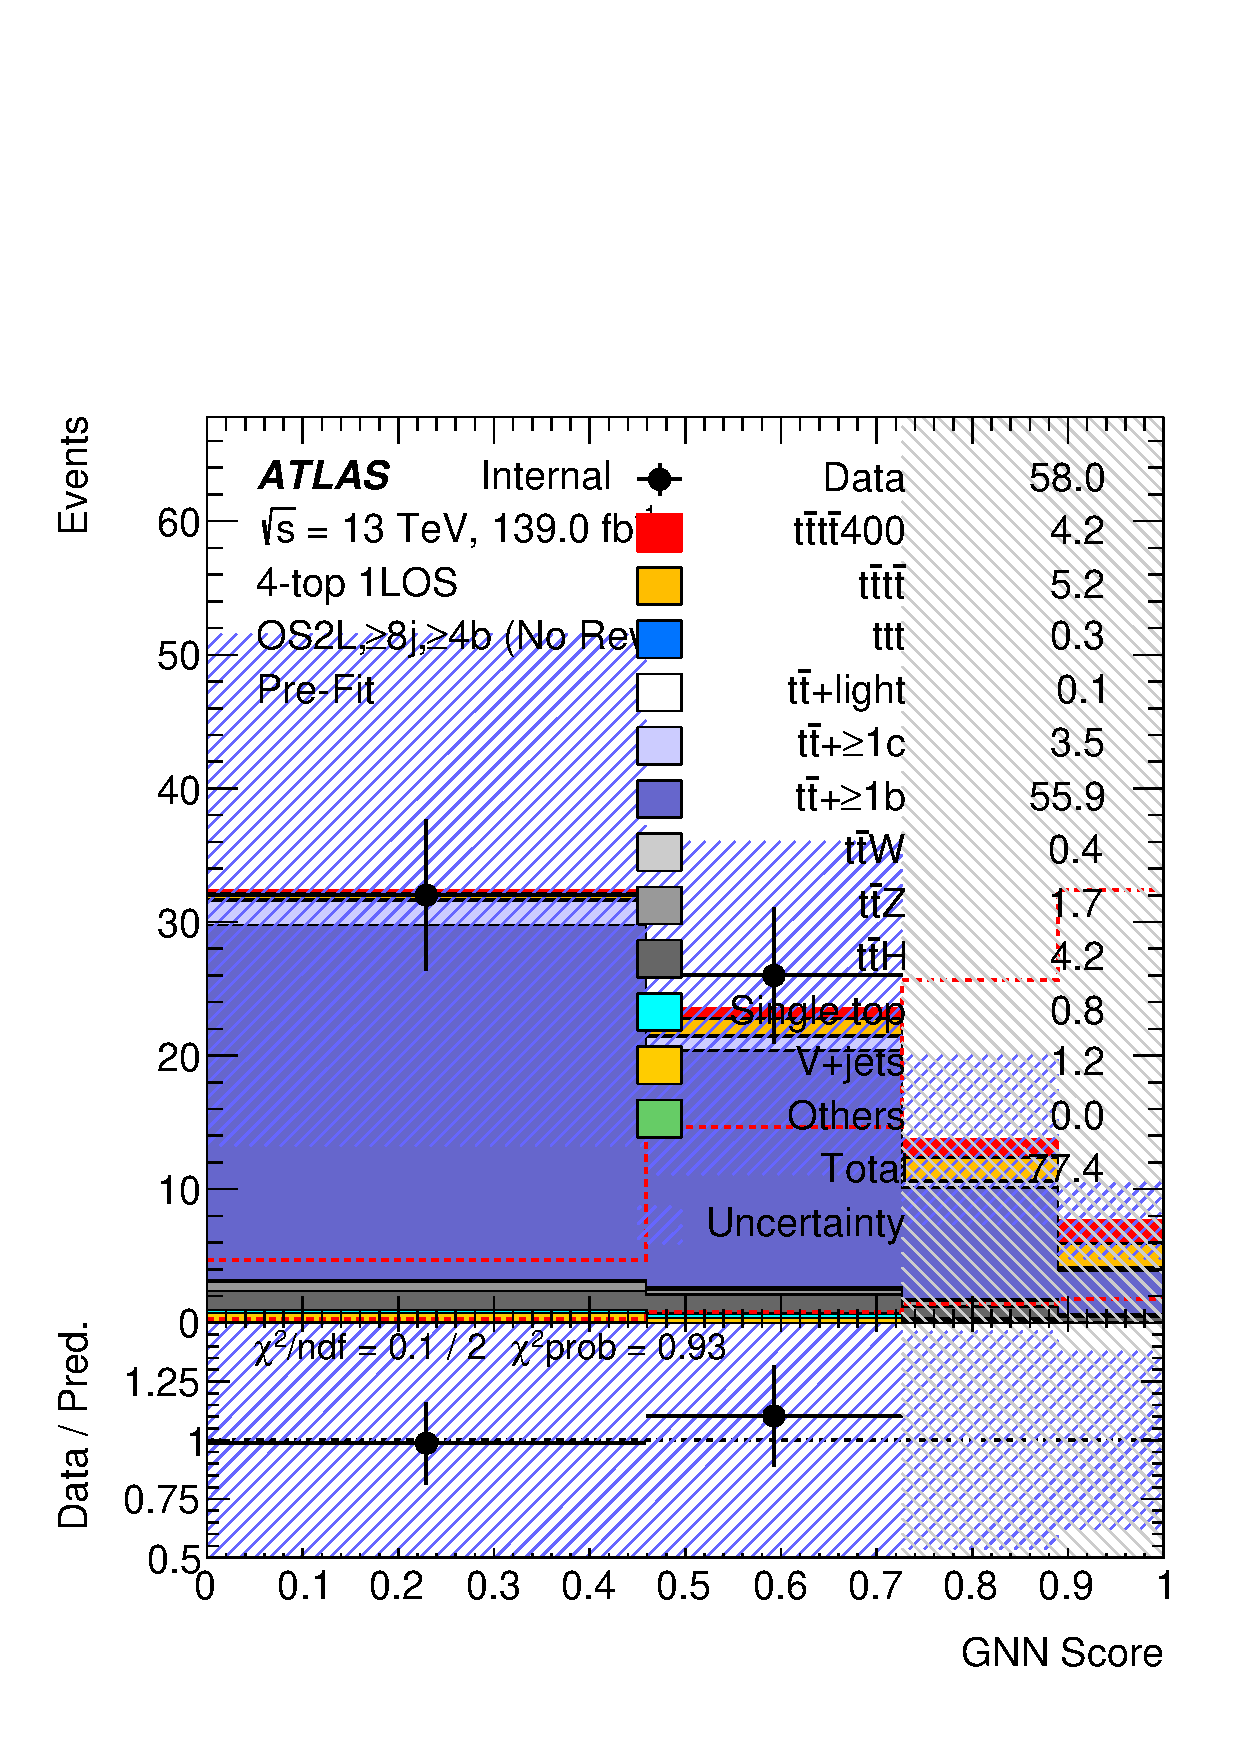
\includegraphics[width=0.4\textwidth]{figures/NNPlots/analysisRegion/NoRew/os2l_ge8jge4b_SR.pdf}
    
\includegraphics[width=0.4\textwidth]{figures/NNPlots/analysisRegion/Rew/os2l_ge8jge4b_SR.pdf}
    \caption{ge8jge4b}
    \end{center}
    \end{subfigure}
    \caption{\label{fig:NNPlots_AnaReg_5} The comparison between variables distribution before (left) and after (right) the NN-reweighting in 2LOS $\geq 8j$ regions.}  
\end{figure}

\clearpage

\begin{table}
\begin{center}
\begin{tabular}{|c|c|c|c|c|c|c|c|c|}
\hline \hline
& 8j3bL & 8j3bH & 8j3bV & 8j4b & 8jge5b & 9j3bL & 9j3bH & 9j3bV \\
\hline
TTL & 0.99 & 1.00 & 0.99 & 0.99 & 1.00 & 0.99 & 0.99 & 0.97 \\
TTC & 0.97 & 0.97 & 0.97 & 0.98 & 1.00 & 0.97 & 0.97 & 0.97 \\
TTB & 0.96 & 0.96 & 0.96 & 0.96 & 0.95 & 0.96 & 0.96 & 0.96 \\
\hline \hline
\end{tabular}

\begin{tabular}{|c|c|c|c|c|c|c|c|c|}
\hline \hline
& 9j4b & 9jge5b & ge10j3bL & ge10j3bH & ge10j4b & ge10jge5b \\
\hline
TTL & 0.95 & 1.00 & 1.06 & 1.00 & 1.05 & 1.00 \\
TTC & 0.98 & 1.00 & 1.04 & 1.05 & 1.05 & 1.00 \\
TTB & 0.96 & 0.94 & 1.03 & 1.03 & 1.03 & 1.03 \\
\hline \hline
\end{tabular}

\begin{tabular}{|c|c|c|c|c|c|c|c|}
\hline \hline
& 6j3bL & 6j3bH & 6j3bV & 6jge4b & 7j3bL & 7j3bH & 7j3bV \\
\hline
TTL & 0.96 & 1.00 & 0.98 & 1.17 & 0.95 & 1.00 & 0.95 \\
TTC & 0.97 & 0.98 & 0.97 & 0.97 & 0.94 & 0.95 & 0.93 \\
TTB & 0.97 & 0.96 & 0.96 & 0.96 & 0.94 & 0.93 & 0.93 \\
\hline \hline
\end{tabular}

\begin{tabular}{|c|c|c|c|c|}
\hline \hline
& 7jge4b & ge8j3bL & ge8j3bH & ge8jge4b \\
\hline
TTL & 1.00 & 1.10 & 0.75 & 1.00 \\
TTC & 0.92 & 1.06 & 1.03 & 1.06 \\
TTB & 0.93 & 1.05 & 1.05 & 1.04 \\
\hline \hline
\end{tabular}

\caption{The yield ratio of after NN-reweighting to before NN-reweighting in 1L regions (8j, 9j and ge10j) and 2LOS regions (6j, 7j and ge8j).}
\label{tab:Rew_NoRew_YieldsRatio}
\end{center}
\end{table}
%%%
\clearpage

%%% MVA Training Regions %%%
\subsection{MVA Training Regions (ge9j(ge7j)ge3b)}
\begin{figure}[htbp!]
    \begin{subfigure}[t]{1\textwidth}
    \begin{center}
    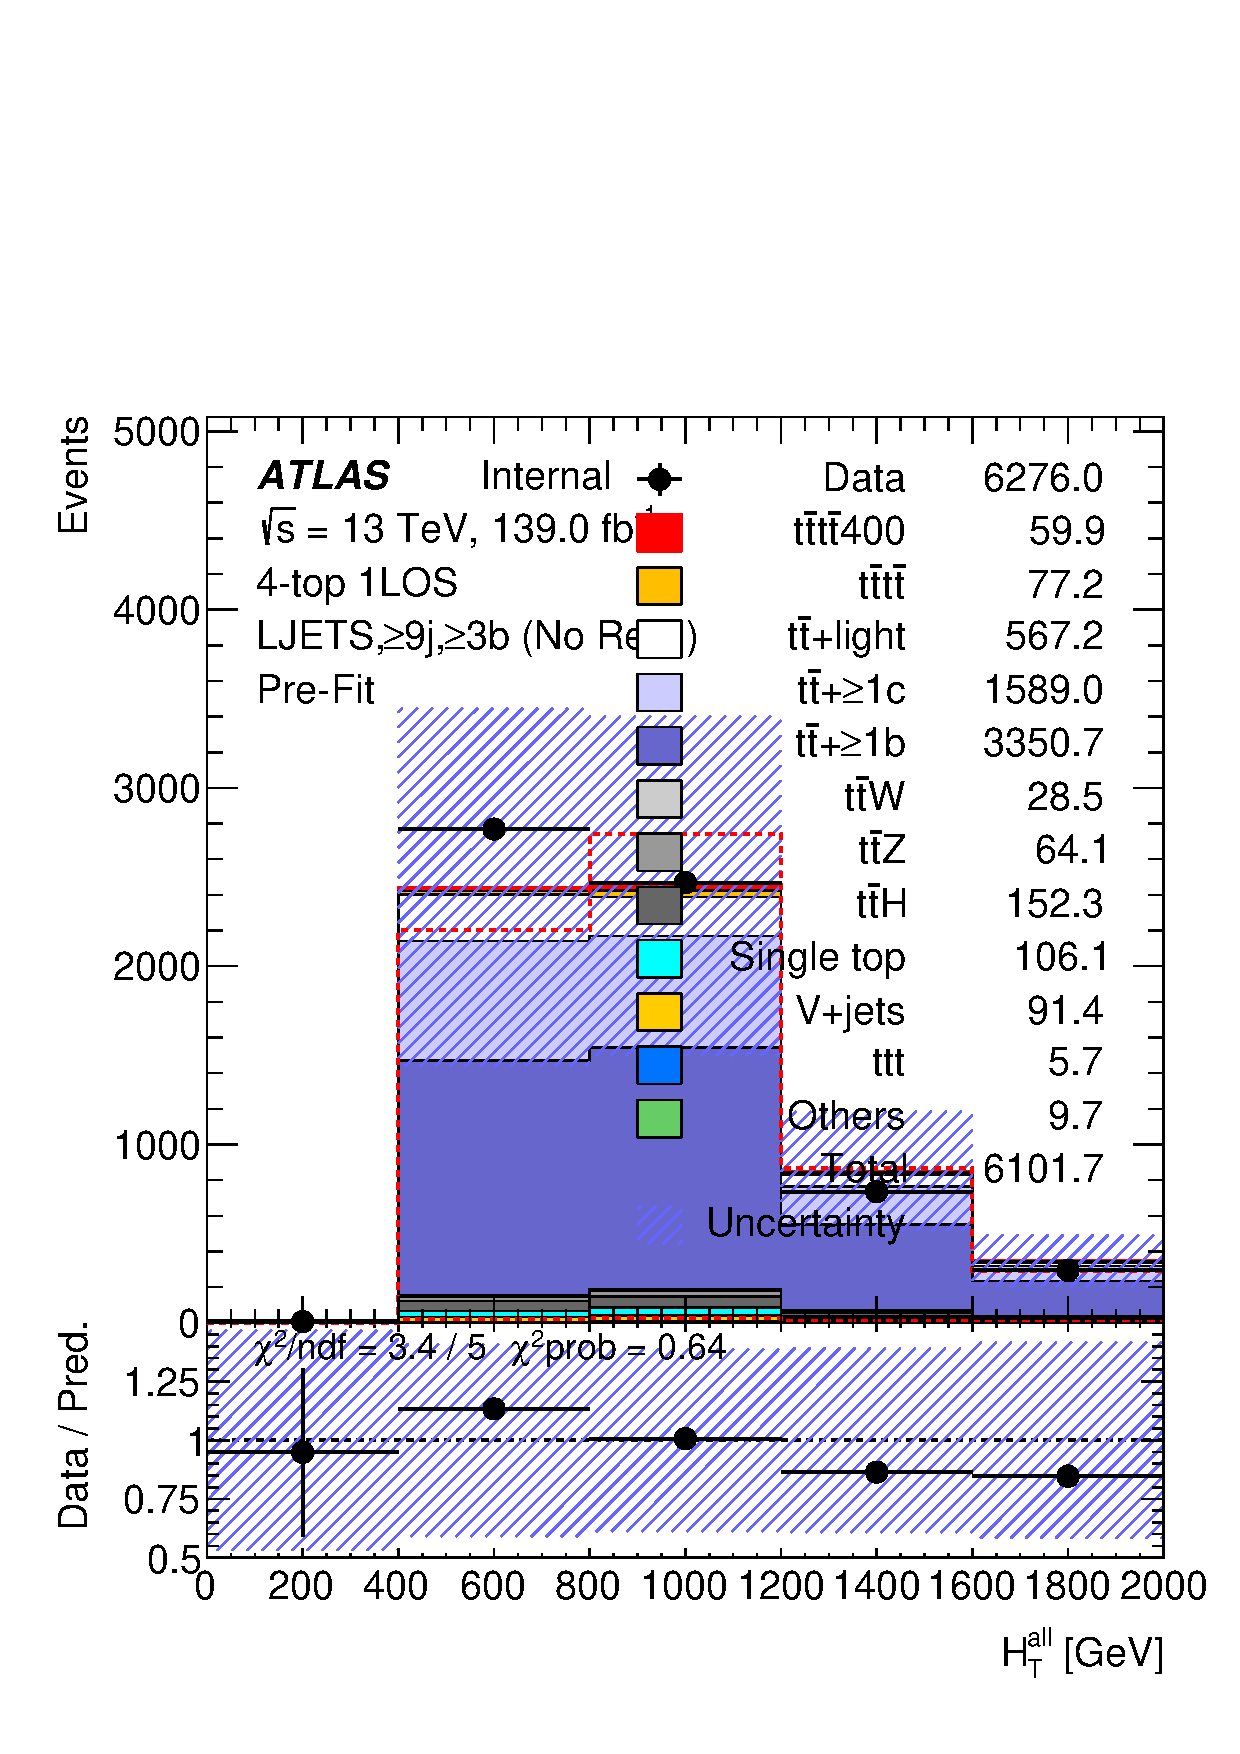
\includegraphics[width=0.3\textwidth]{figures/NNPlots/MVATrainRegion/NoRew/ljets_ge9jge3b_HT.pdf}
    
\includegraphics[width=0.3\textwidth]{figures/NNPlots/MVATrainRegion/Rew/ljets_ge9jge3b_HT.pdf}
    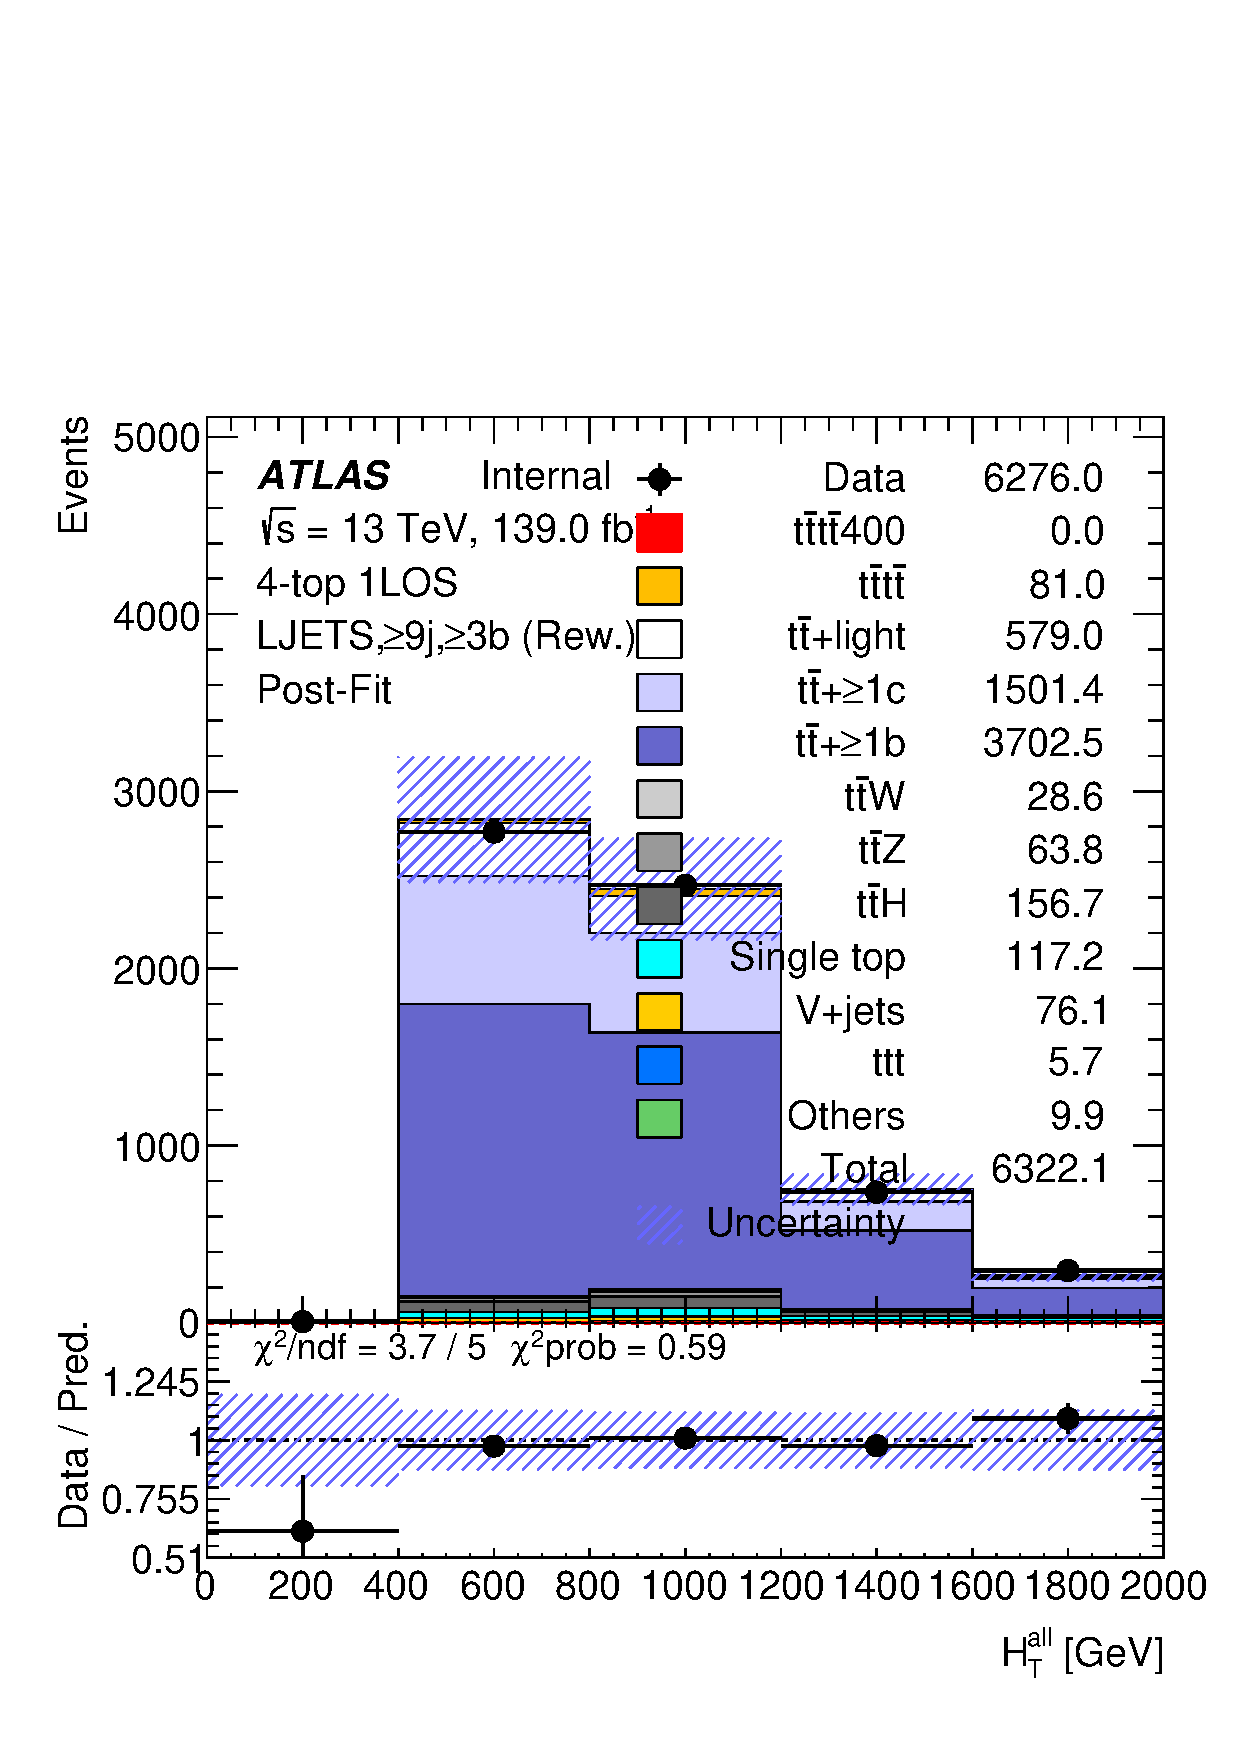
\includegraphics[width=0.3\textwidth]{figures/NNPlots/MVATrainRegion/Rew/ljets_ge9jge3b_HT_postFit.pdf}
    \caption{$H_{T}$}
    \end{center}
    \end{subfigure}

    \begin{subfigure}[t]{1\textwidth}
    \begin{center}
    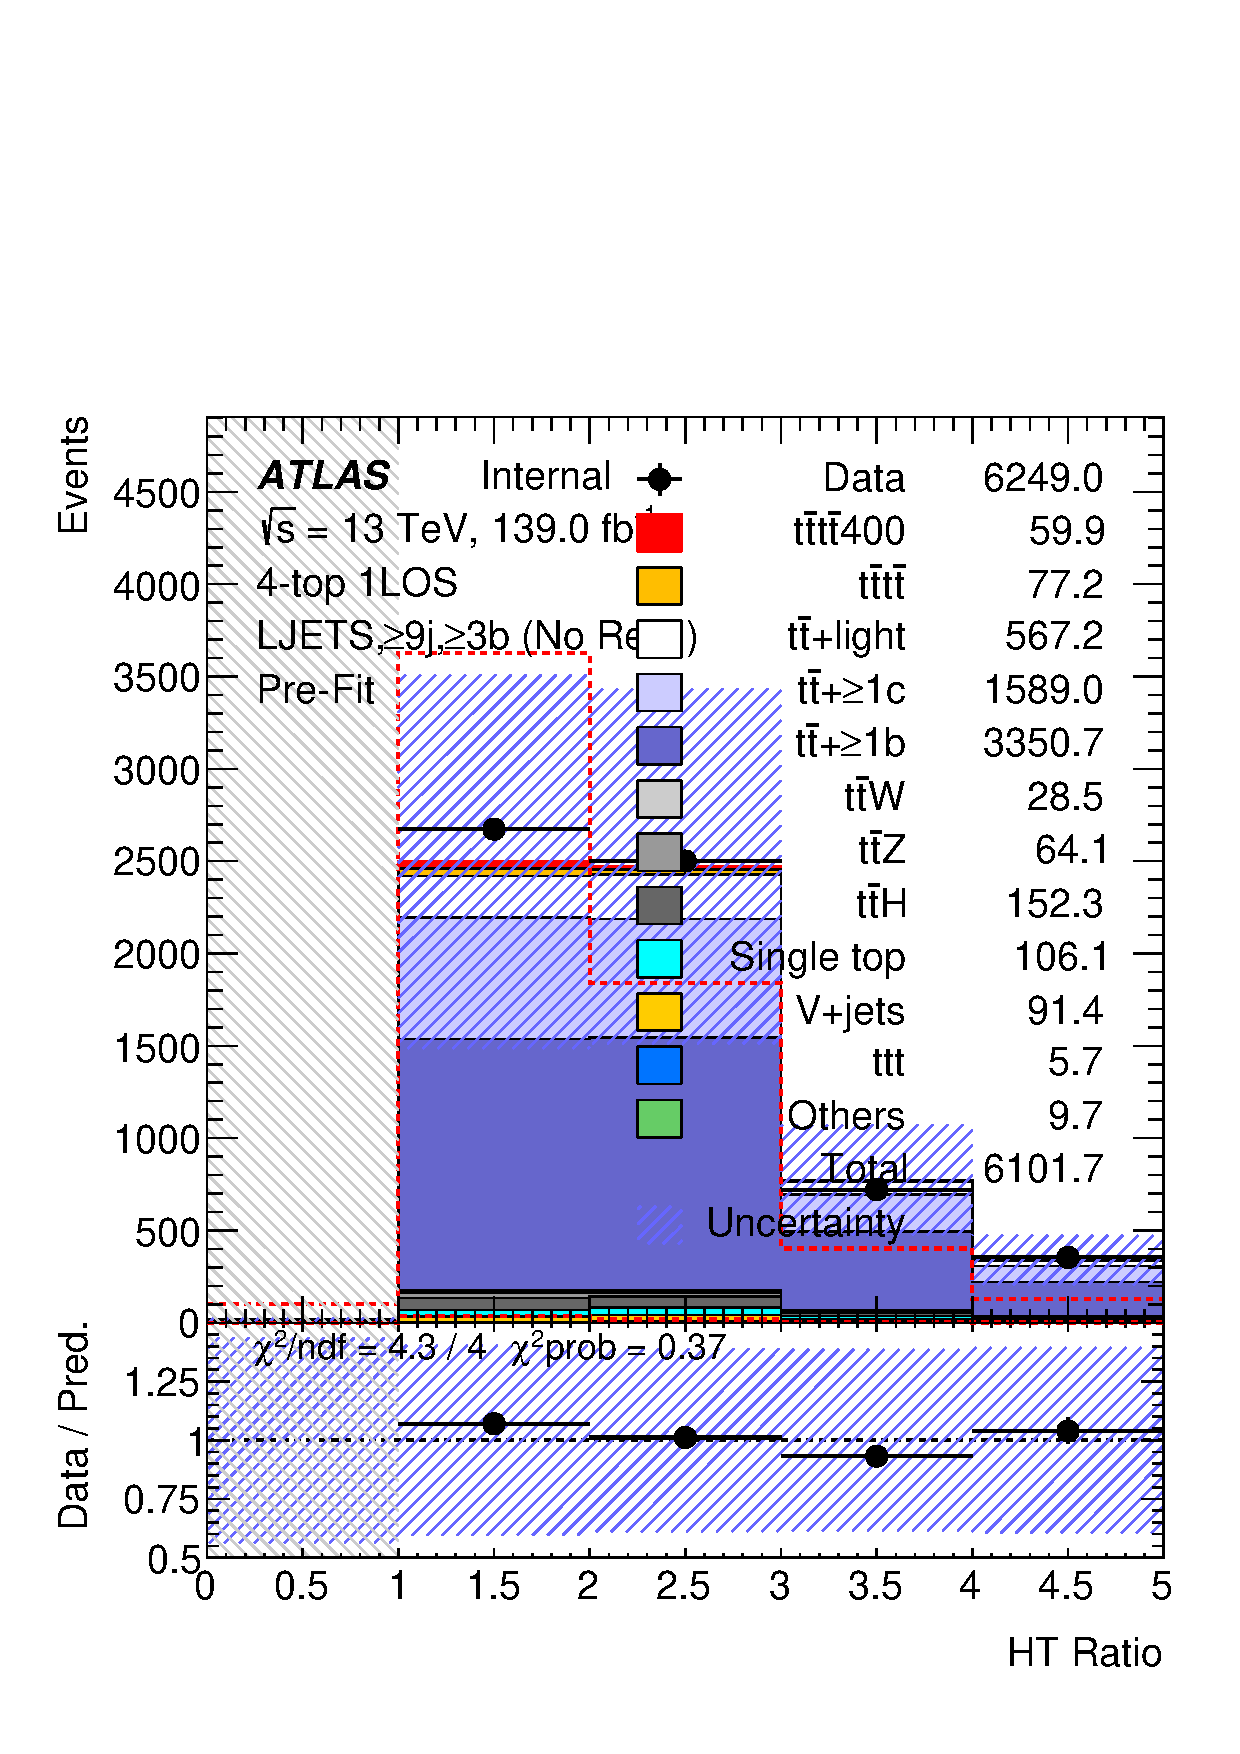
\includegraphics[width=0.3\textwidth]{figures/NNPlots/MVATrainRegion/NoRew/ljets_ge9jge3b_HTRatio.pdf}
    
\includegraphics[width=0.3\textwidth]{figures/NNPlots/MVATrainRegion/Rew/ljets_ge9jge3b_HTRatio.pdf}
    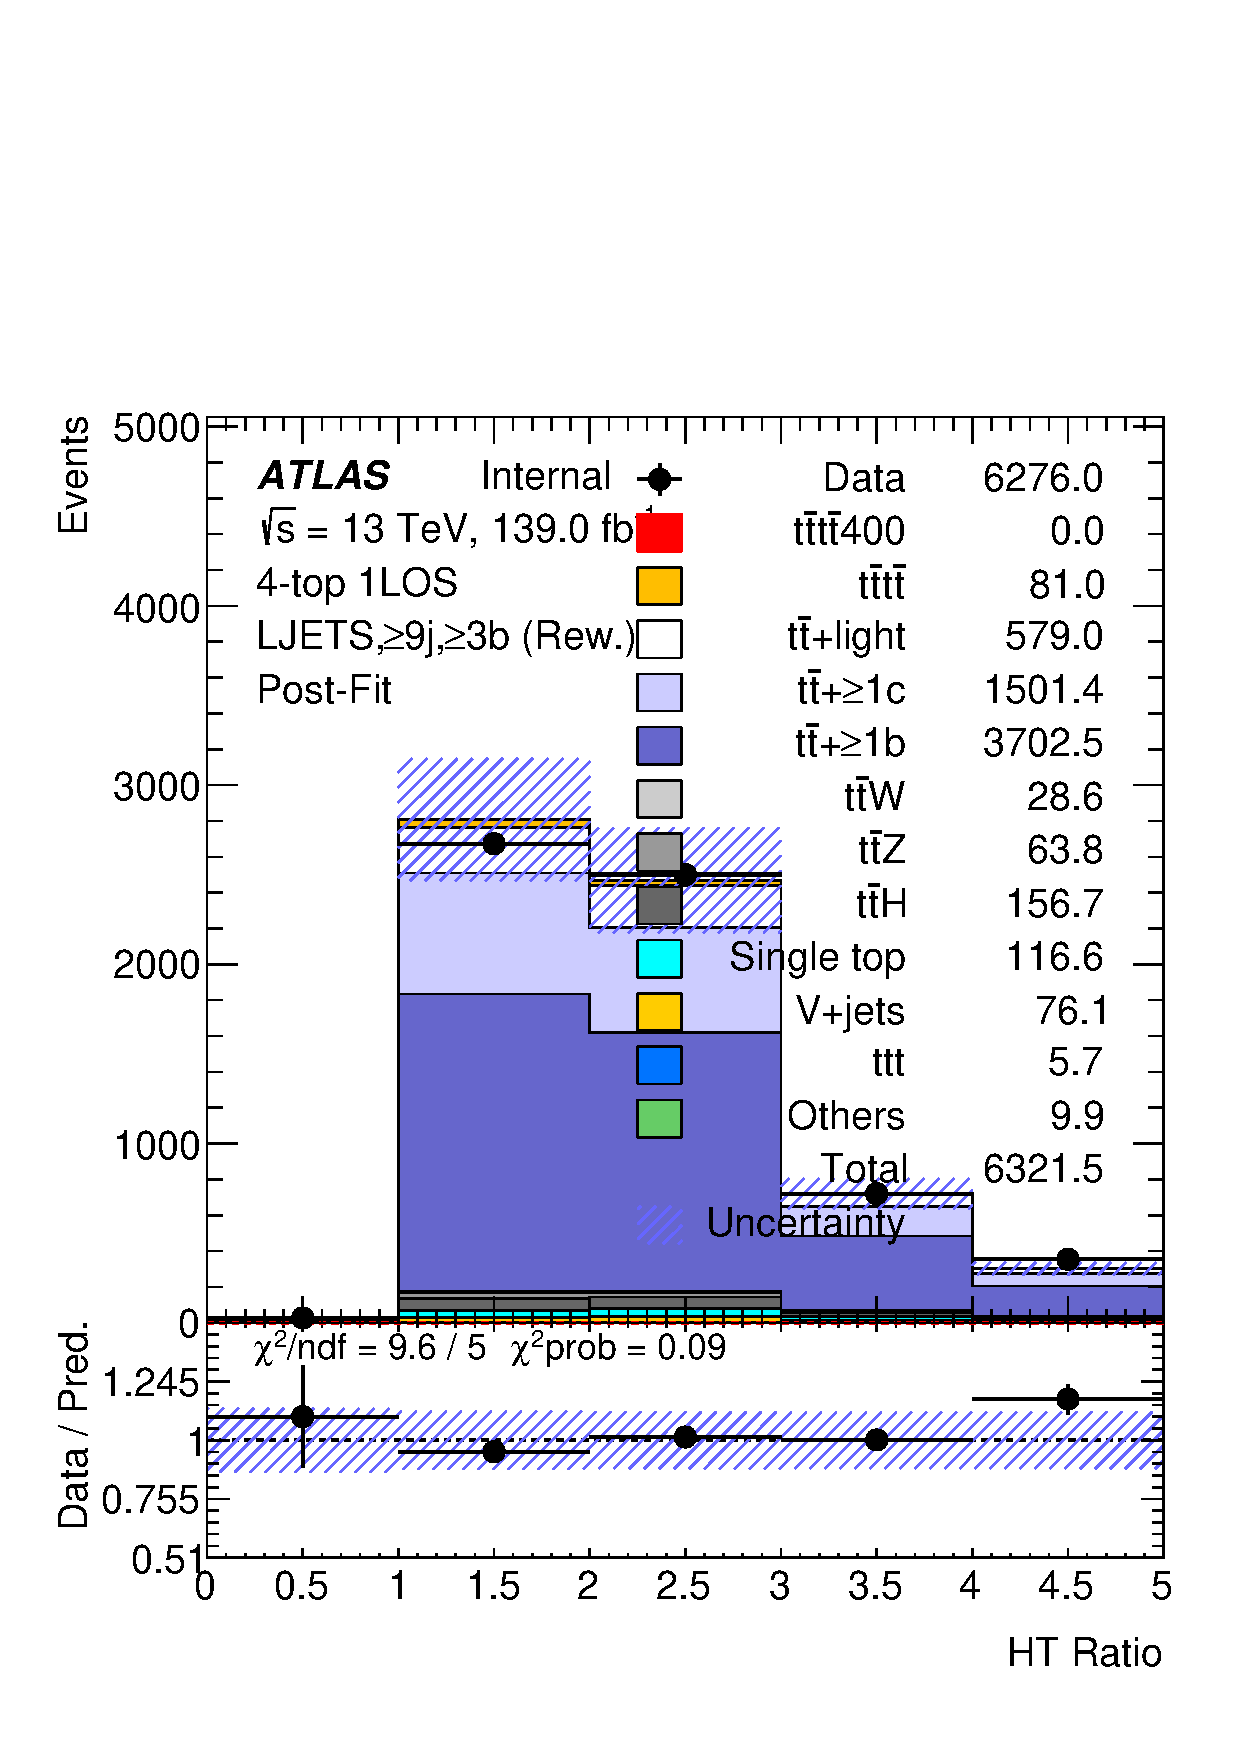
\includegraphics[width=0.3\textwidth]{figures/NNPlots/MVATrainRegion/Rew/ljets_ge9jge3b_HTRatio_postFit.pdf}
    \caption{HTRatio}
    \end{center}
    \end{subfigure}

    \begin{subfigure}[t]{1\textwidth}
    \begin{center}
    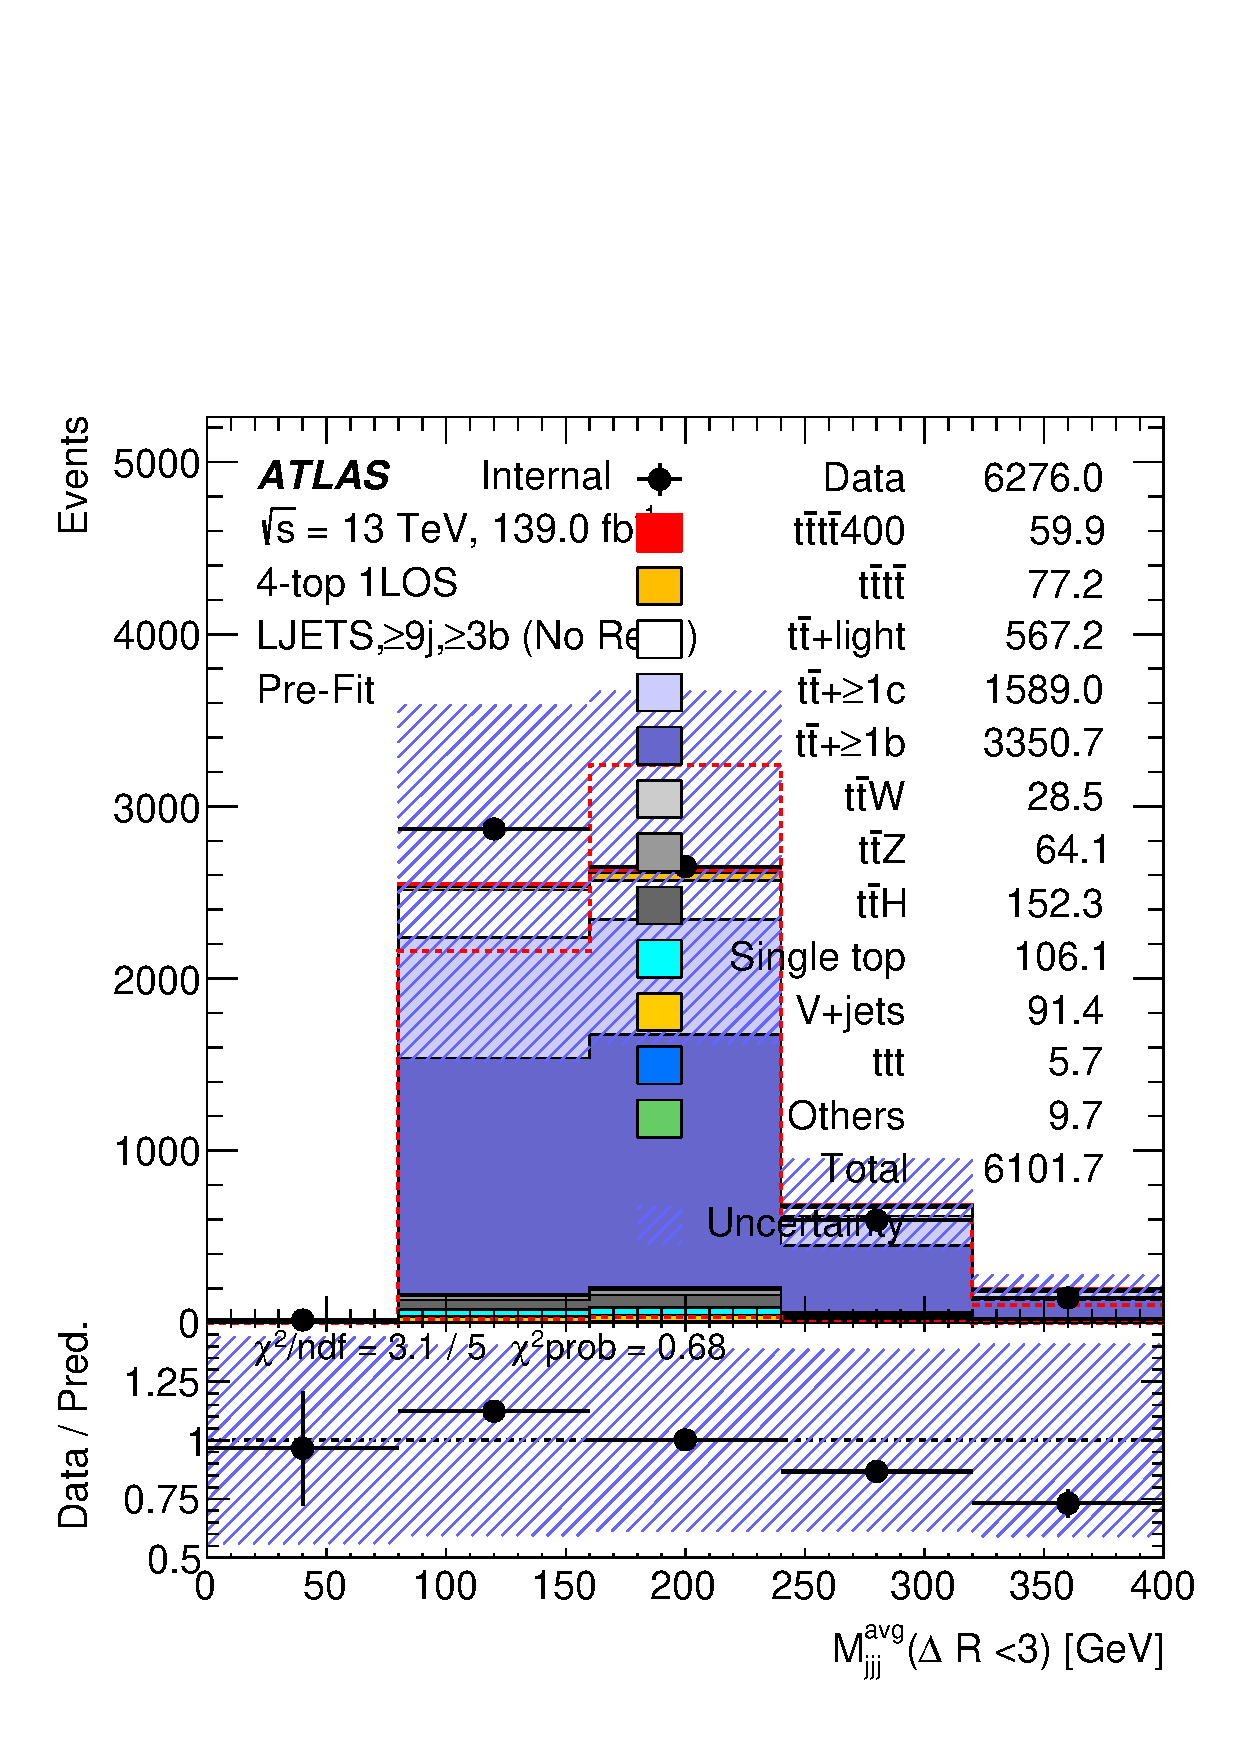
\includegraphics[width=0.3\textwidth]{figures/NNPlots/MVATrainRegion/NoRew/ljets_ge9jge3b_Mjjj_AvgdRs3.pdf}
    
\includegraphics[width=0.3\textwidth]{figures/NNPlots/MVATrainRegion/Rew/ljets_ge9jge3b_Mjjj_AvgdRs3.pdf}
    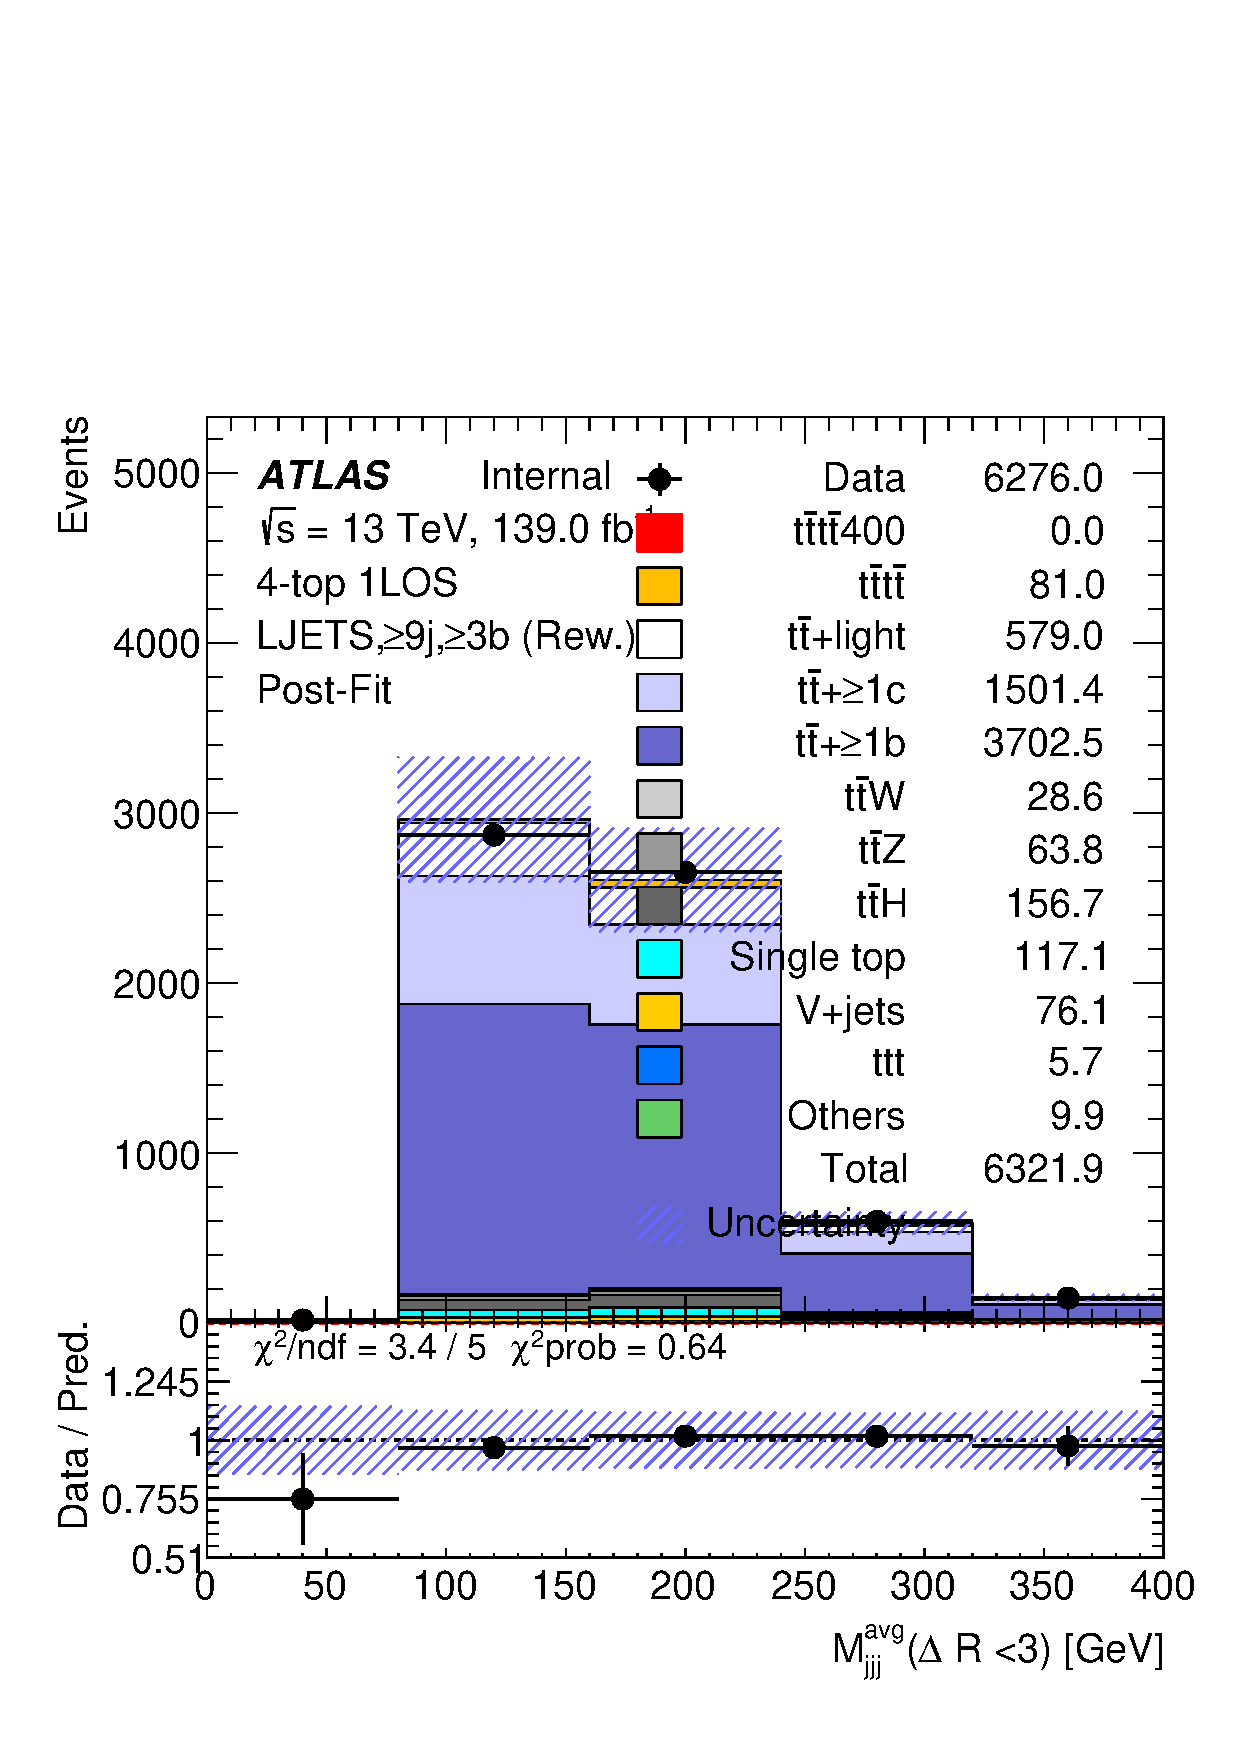
\includegraphics[width=0.3\textwidth]{figures/NNPlots/MVATrainRegion/Rew/ljets_ge9jge3b_Mjjj_AvgdRs3_postFit.pdf}
    \caption{$M^{avg}_{jjj}(\Delta R <3)$}
    \end{center}
    \end{subfigure}
    \caption{\label{fig:NNPlots_MVATrainReg_1} The comparison between variables pre-fit distribution before (left) and after (middle) the NN-reweighting  in 1L MVA training regions ($\geq 9j,\geq 3b$). The post-fit distribution after the NN-reweighting is shown on the left. Blinded regions are excluded.}  
\end{figure}

\begin{figure}[htbp!]
    \begin{subfigure}[t]{1\textwidth}
    \begin{center}
    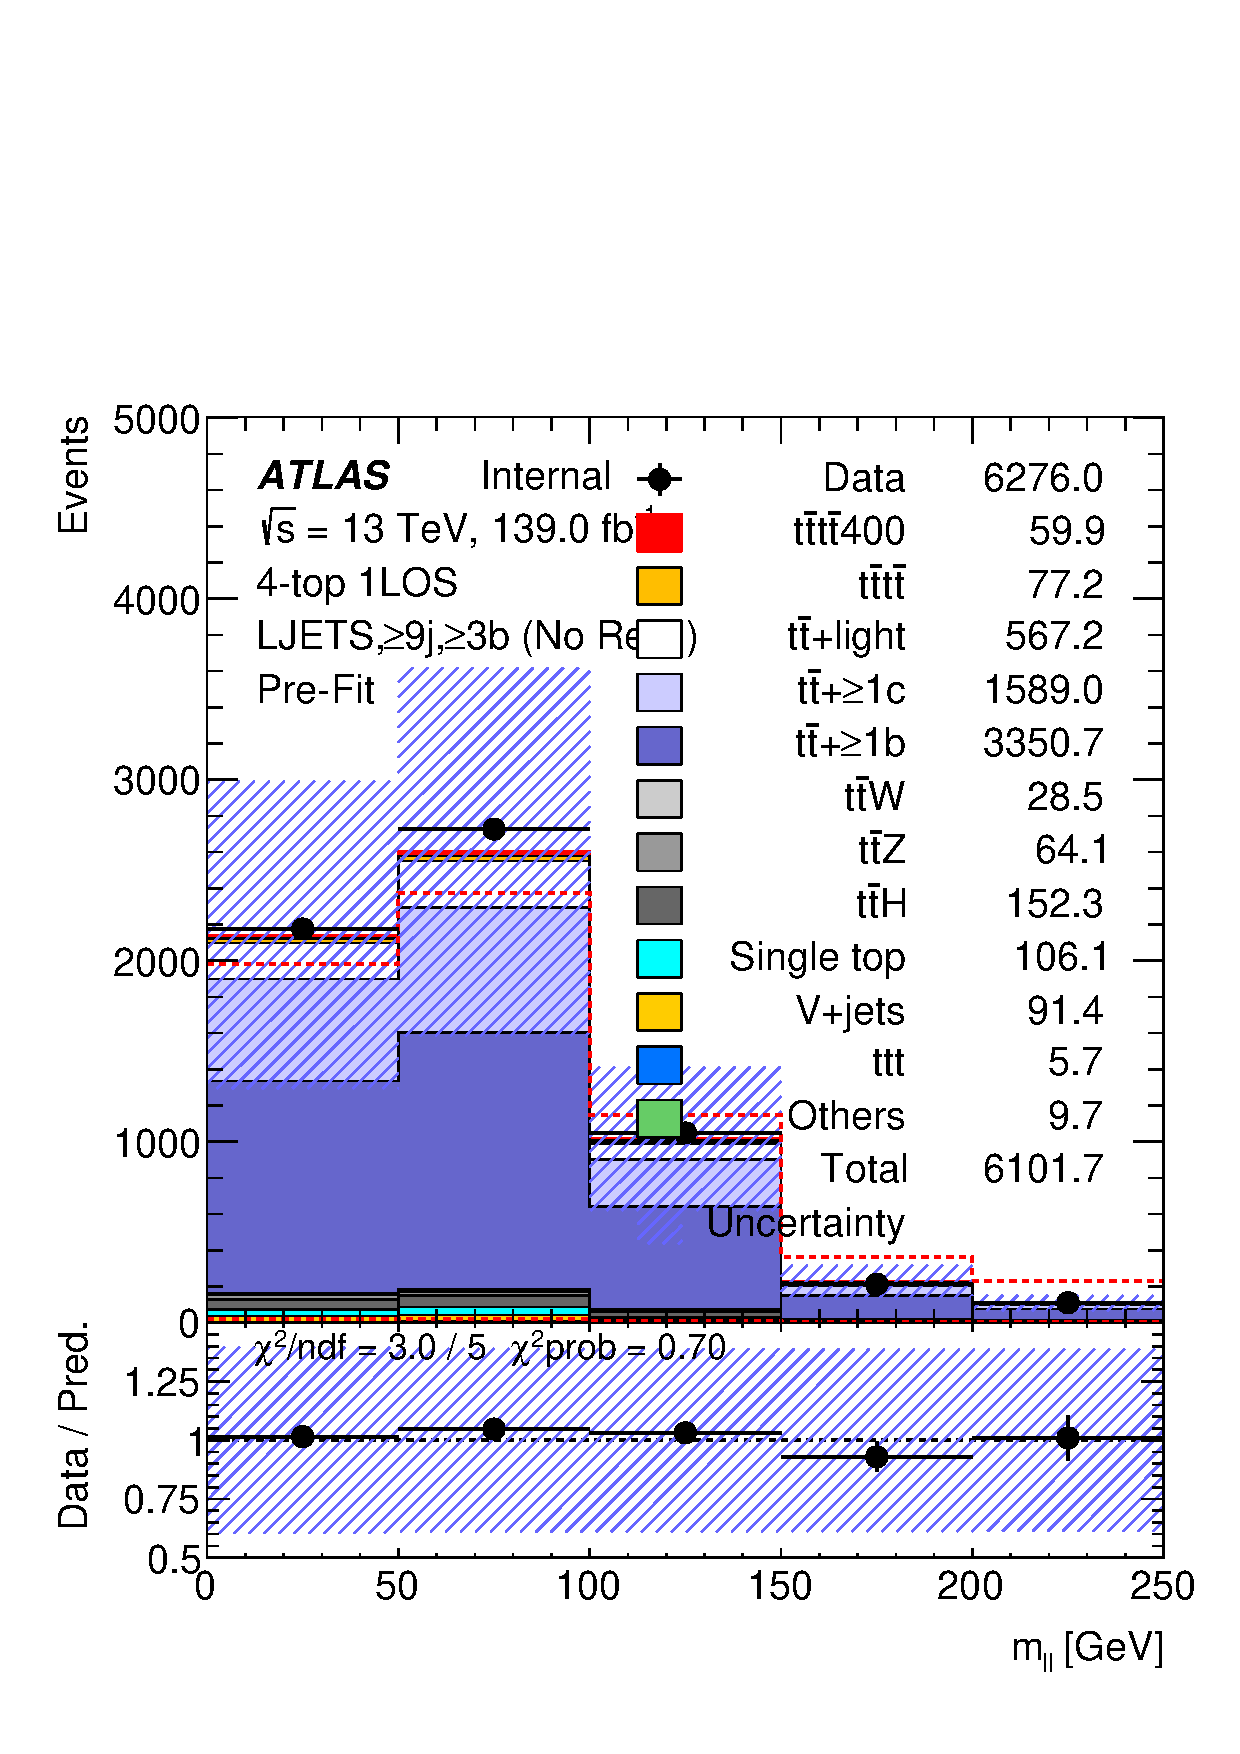
\includegraphics[width=0.3\textwidth]{figures/NNPlots/MVATrainRegion/NoRew/ljets_ge9jge3b_mtw.pdf}
    
\includegraphics[width=0.3\textwidth]{figures/NNPlots/MVATrainRegion/Rew/ljets_ge9jge3b_mtw.pdf}
    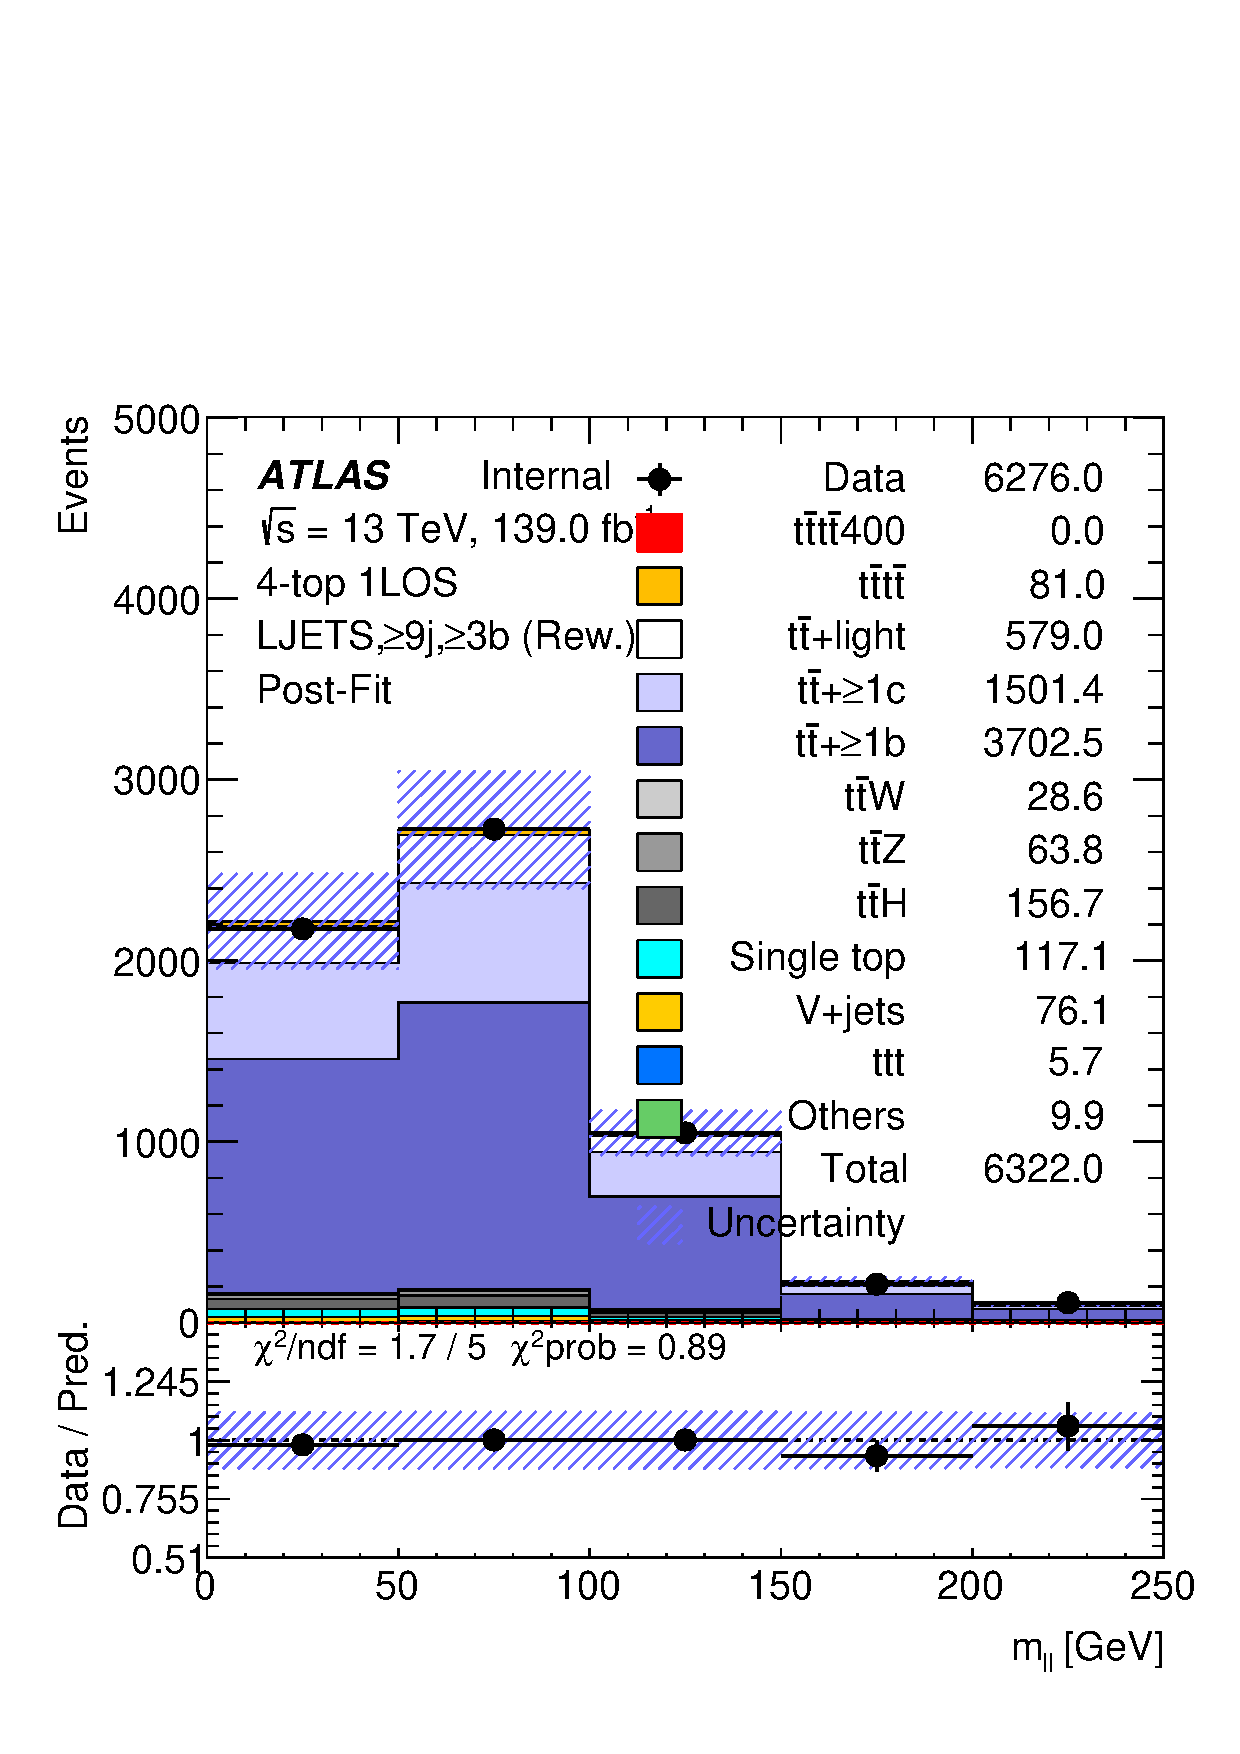
\includegraphics[width=0.3\textwidth]{figures/NNPlots/MVATrainRegion/Rew/ljets_ge9jge3b_mtw_postFit.pdf}
    \caption{mtw}
    \end{center}
    \end{subfigure}

    \begin{subfigure}[t]{1\textwidth}
    \begin{center}
    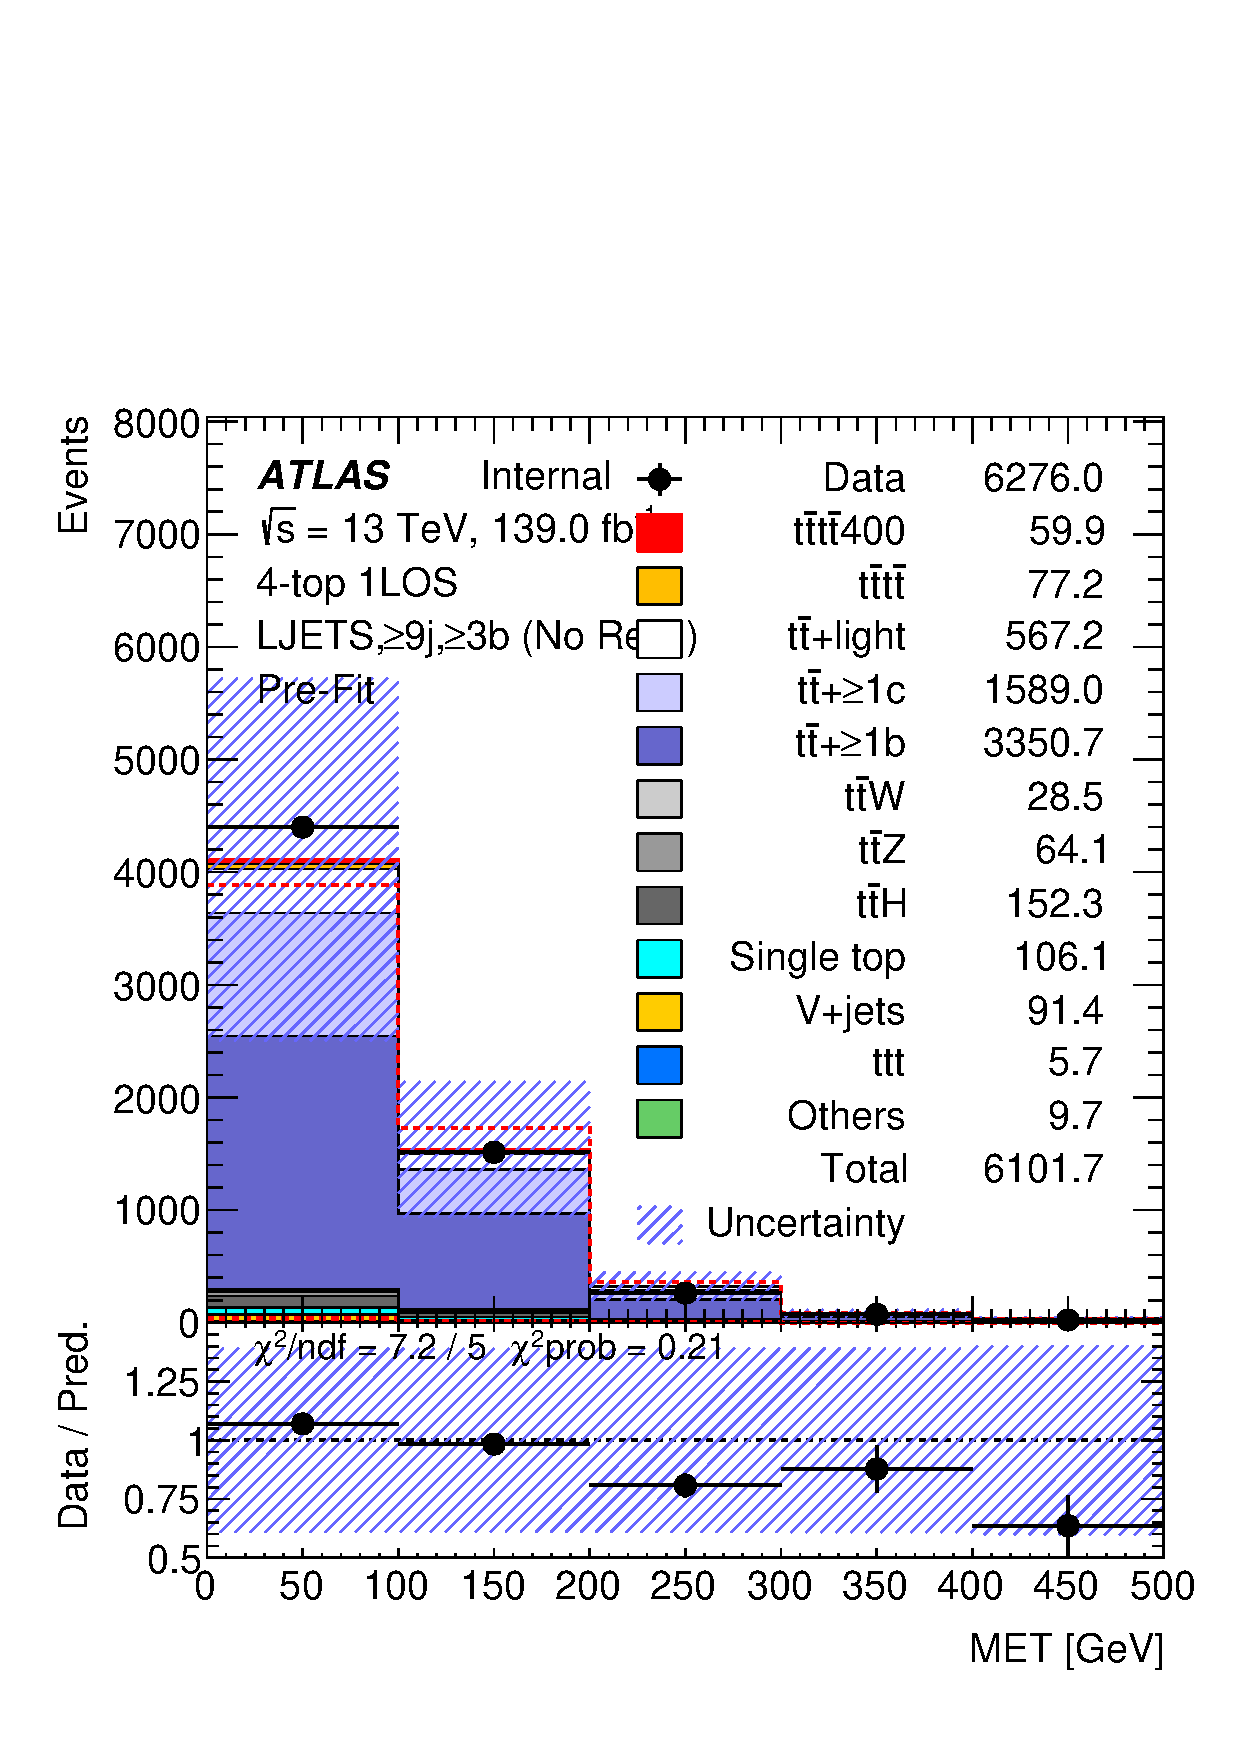
\includegraphics[width=0.3\textwidth]{figures/NNPlots/MVATrainRegion/NoRew/ljets_ge9jge3b_met.pdf}
    
\includegraphics[width=0.3\textwidth]{figures/NNPlots/MVATrainRegion/Rew/ljets_ge9jge3b_met.pdf}
    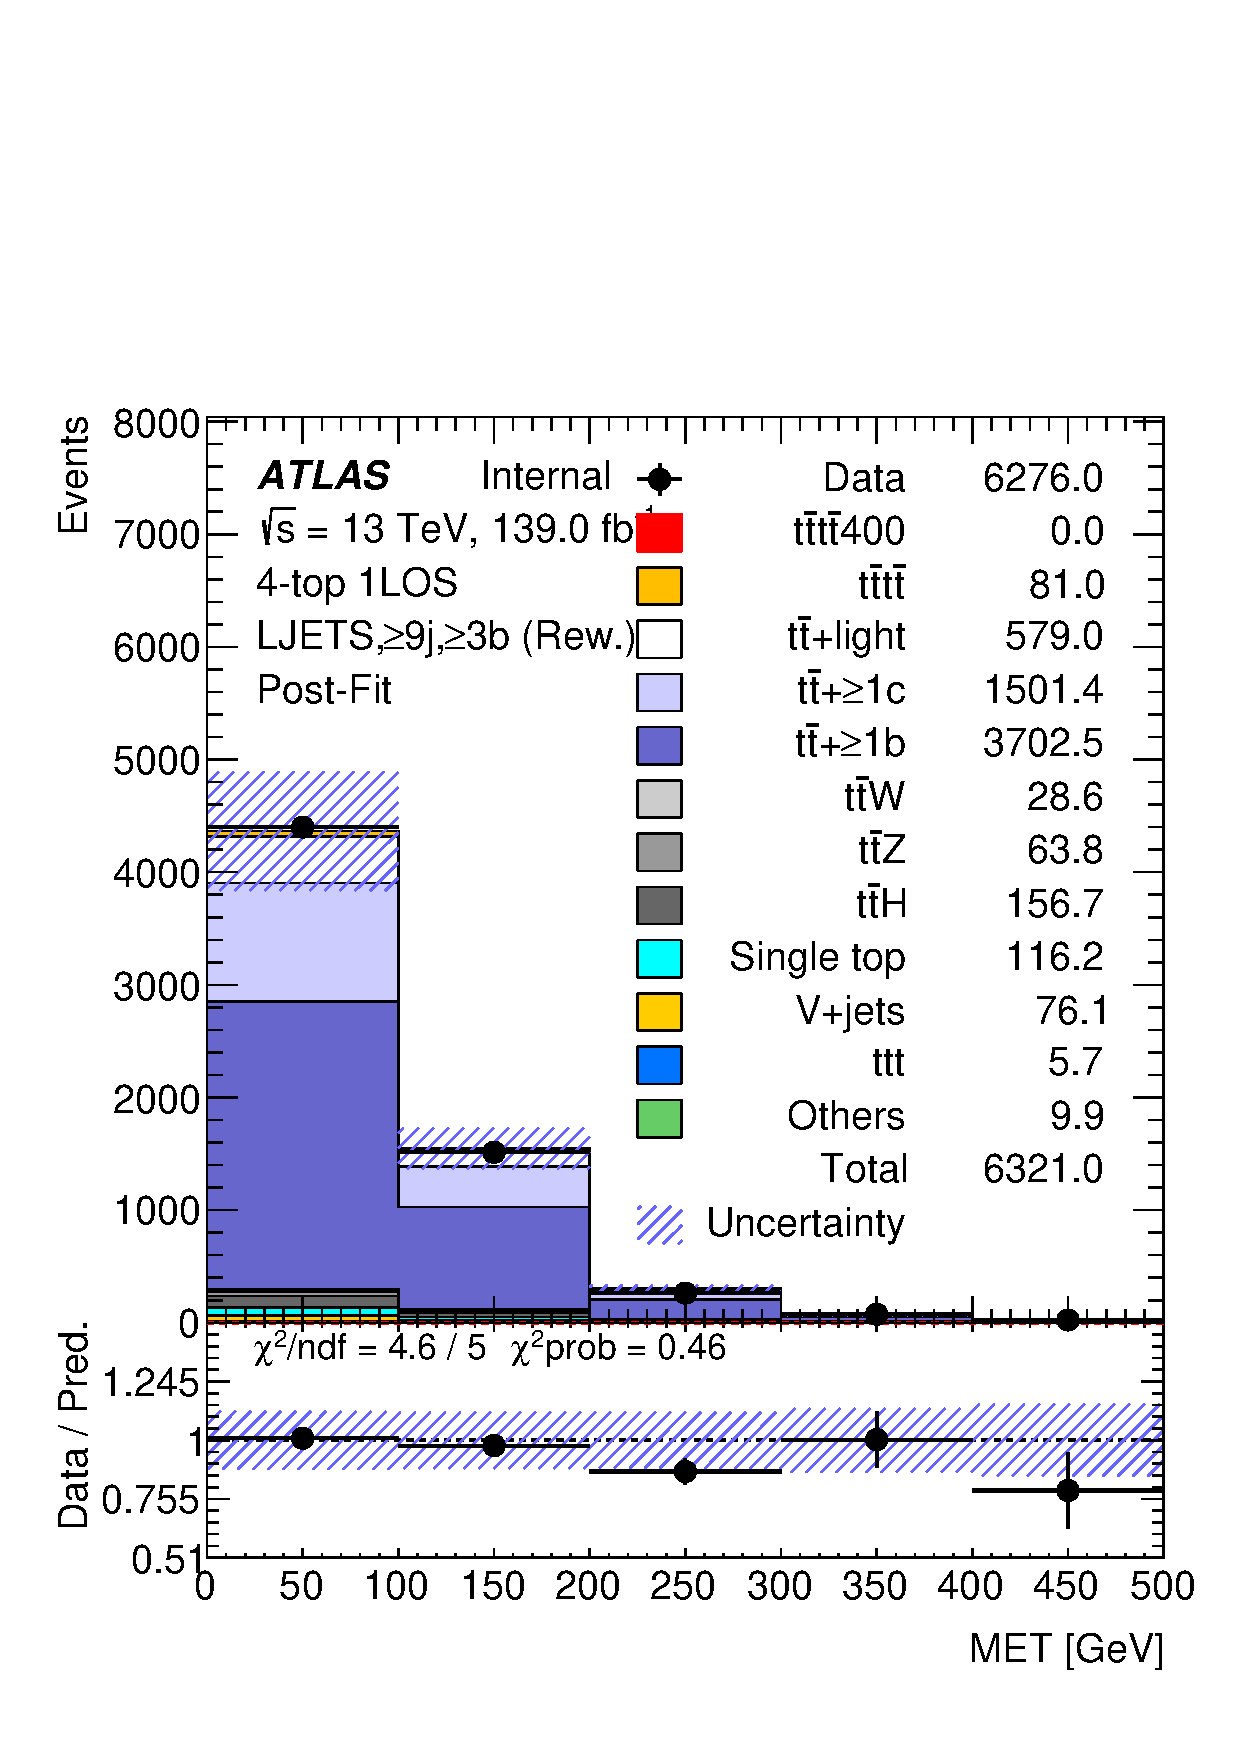
\includegraphics[width=0.3\textwidth]{figures/NNPlots/MVATrainRegion/Rew/ljets_ge9jge3b_met_postFit.pdf}
    \caption{MET}
    \end{center}
    \end{subfigure}

    \begin{subfigure}[t]{1\textwidth}
    \begin{center}
    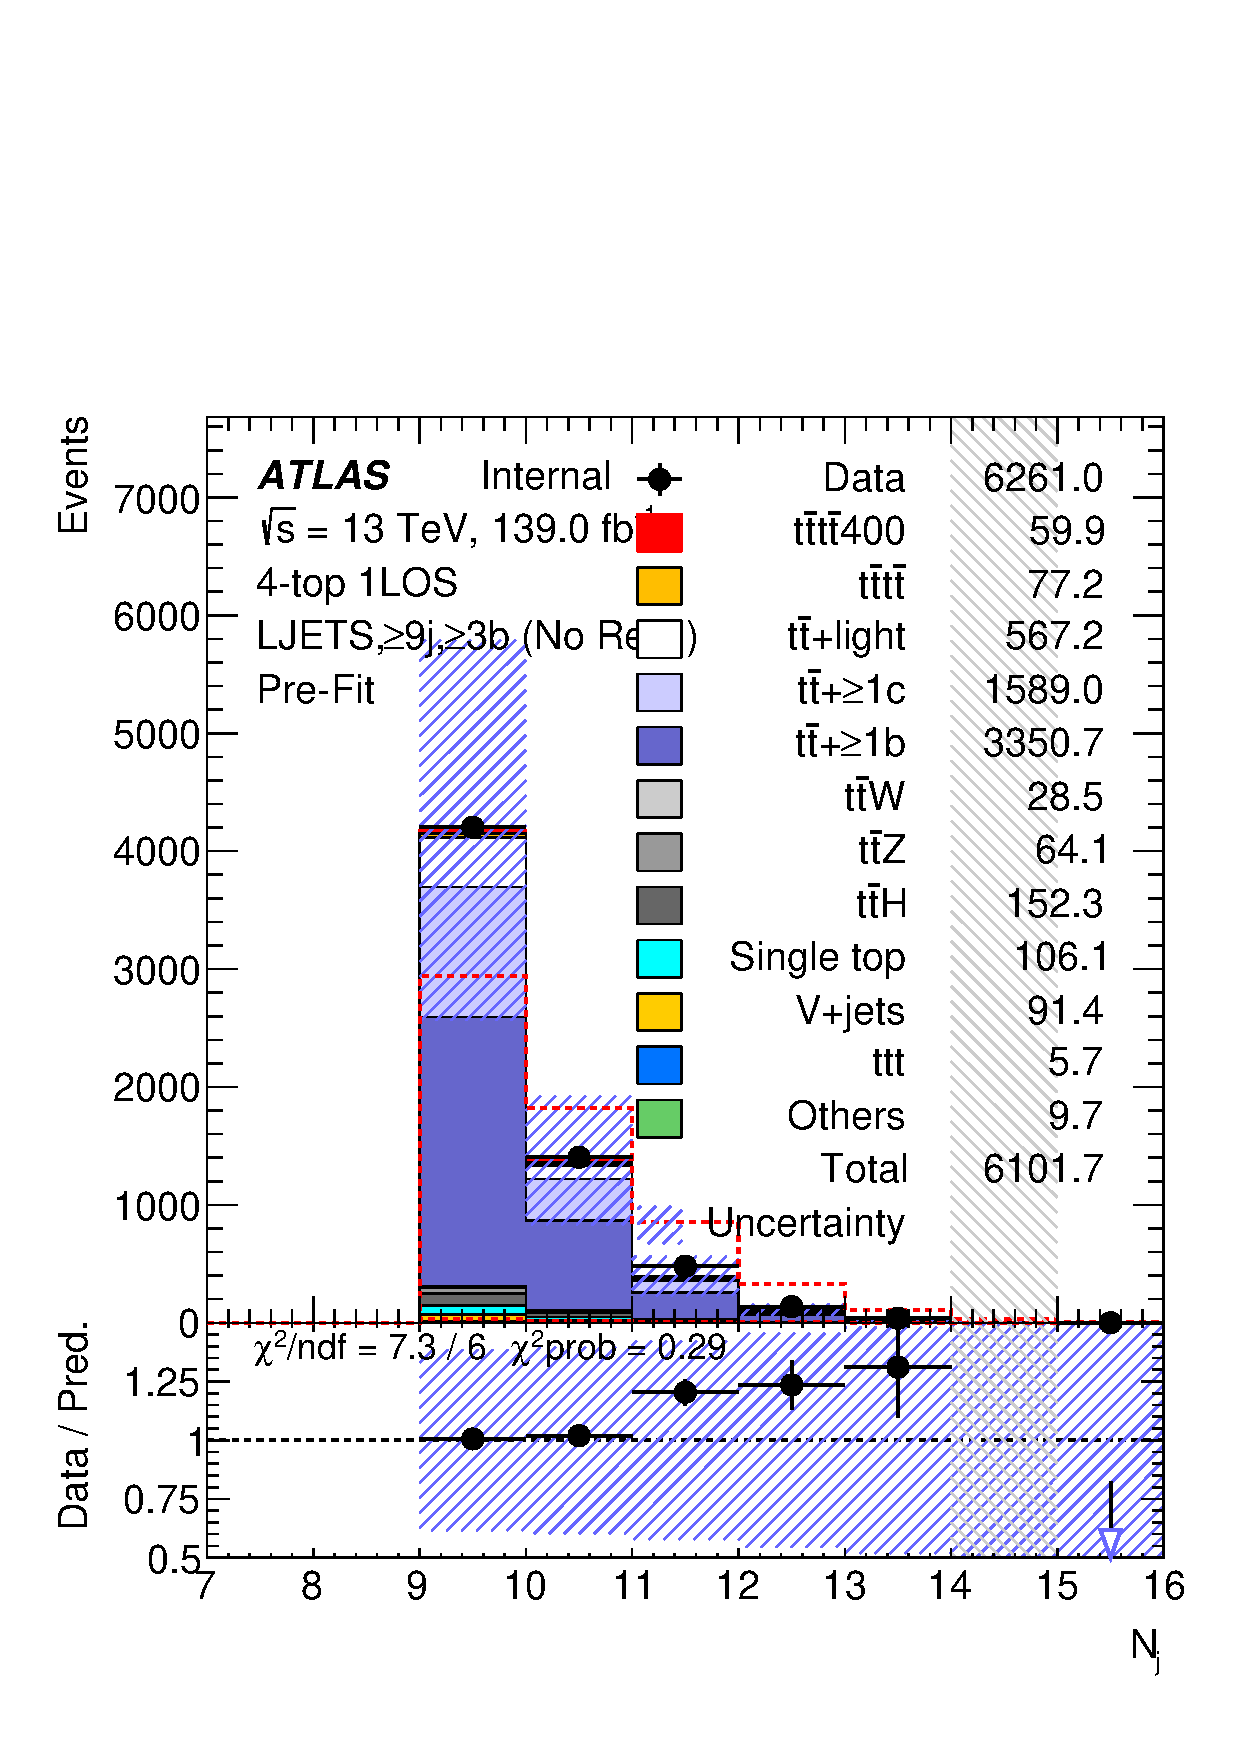
\includegraphics[width=0.3\textwidth]{figures/NNPlots/MVATrainRegion/NoRew/ljets_ge9jge3b_nJets.pdf}
    
\includegraphics[width=0.3\textwidth]{figures/NNPlots/MVATrainRegion/Rew/ljets_ge9jge3b_nJets.pdf}
    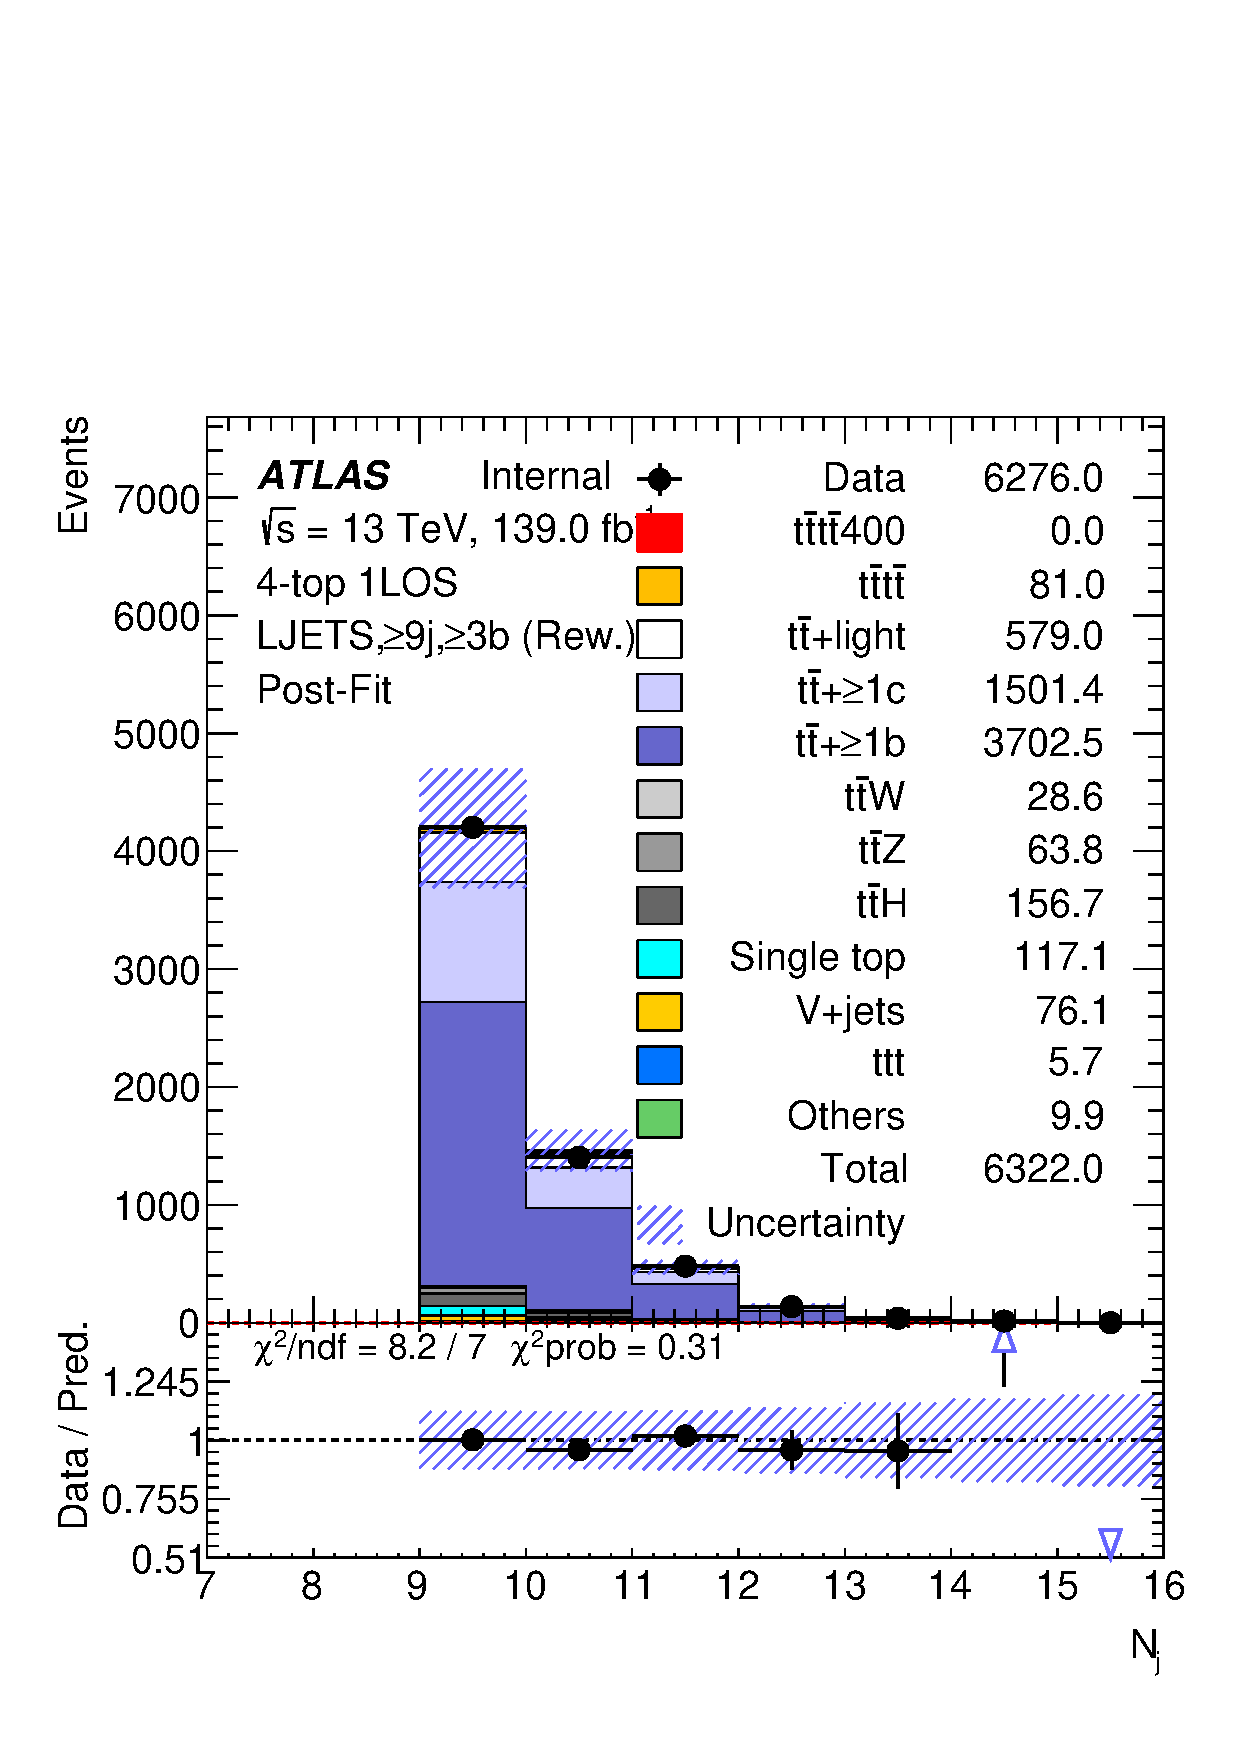
\includegraphics[width=0.3\textwidth]{figures/NNPlots/MVATrainRegion/Rew/ljets_ge9jge3b_nJets_postFit.pdf}
    \caption{nJets}
    \end{center}
    \end{subfigure}
    \caption{\label{fig:NNPlots_MVATrainReg_2} The comparison between variables pre-fit distribution before (left) and after (middle) the NN-reweighting  in 1L MVA training regions ($\geq 9j,\geq 3b$). The post-fit distribution after the NN-reweighting is shown on the left. Blinded regions are excluded.}
\end{figure}

\begin{figure}[htbp!]
    \begin{subfigure}[t]{1\textwidth}
    \begin{center}
    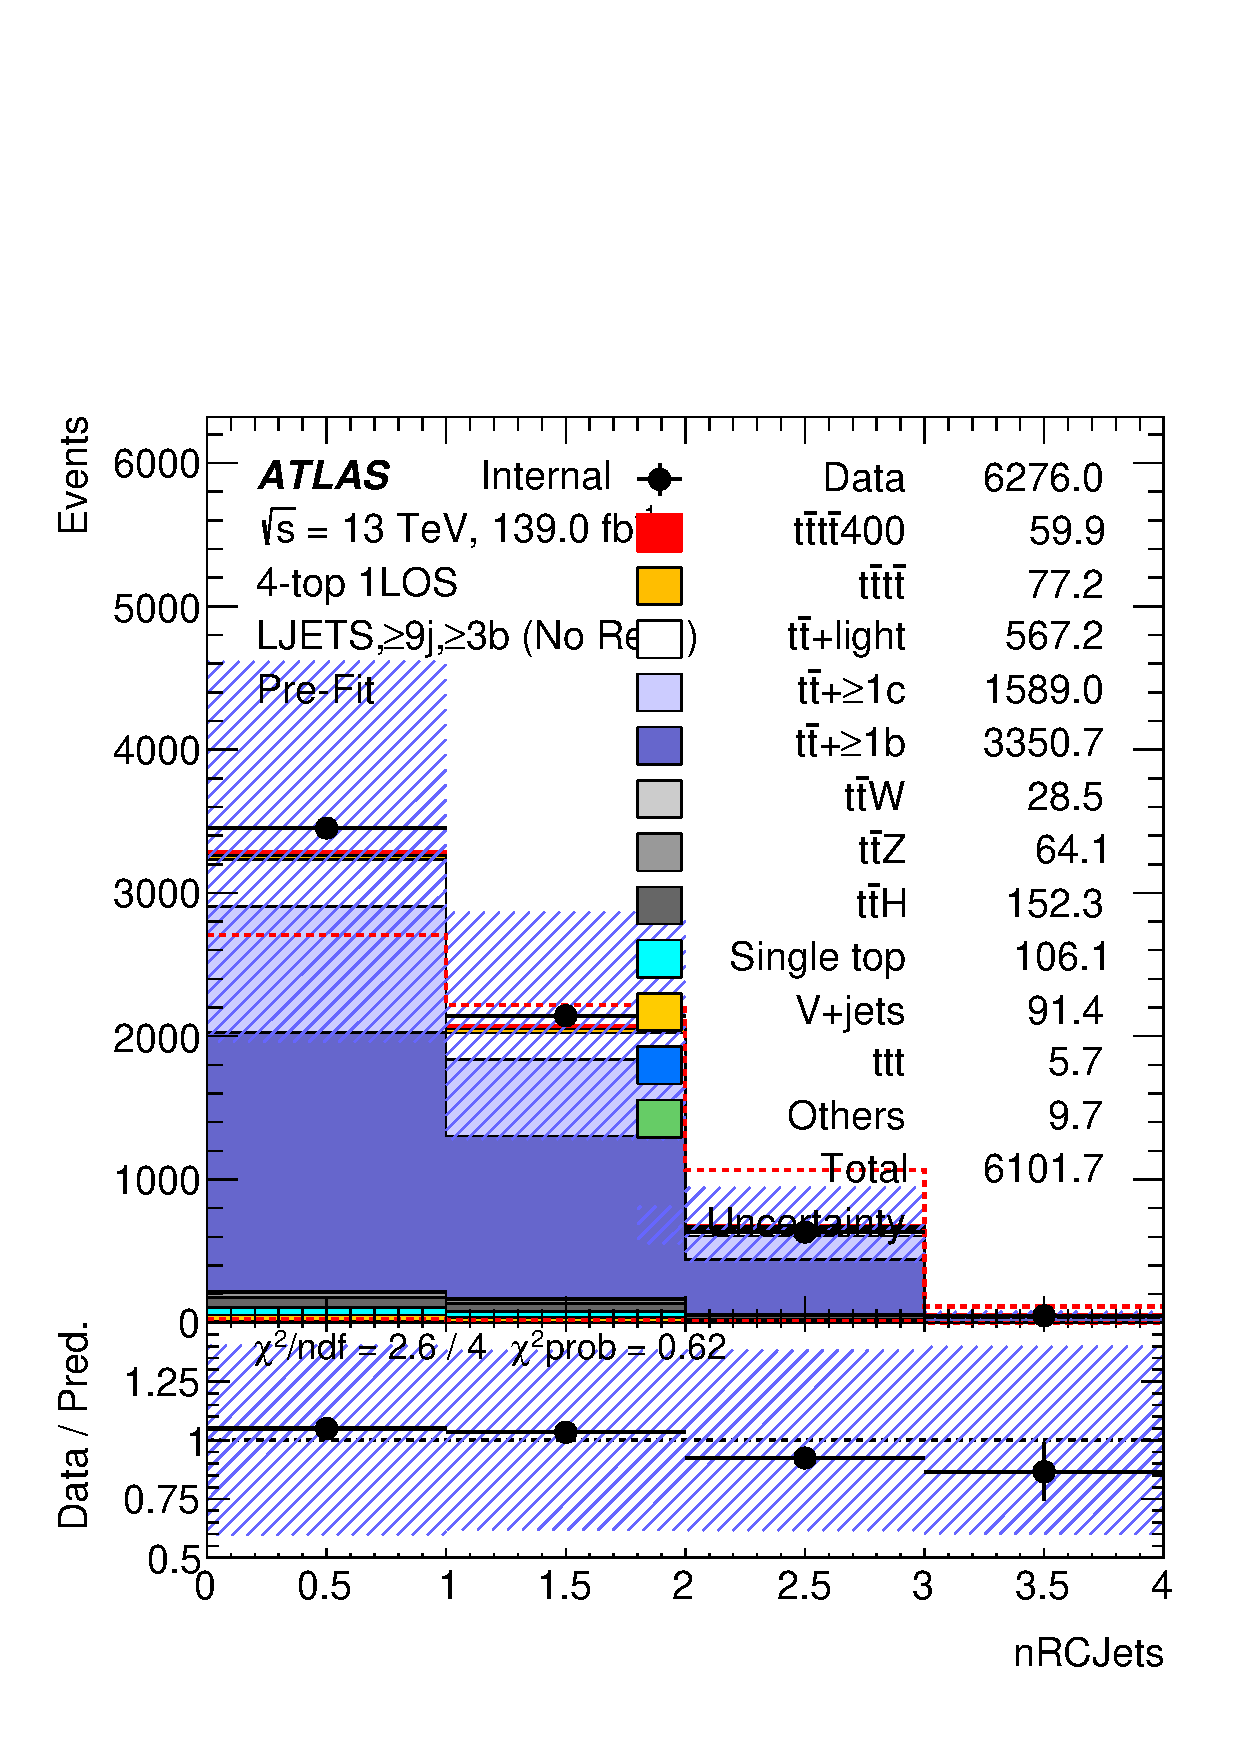
\includegraphics[width=0.3\textwidth]{figures/NNPlots/MVATrainRegion/NoRew/ljets_ge9jge3b_nRCJetsM100.pdf}
    
\includegraphics[width=0.3\textwidth]{figures/NNPlots/MVATrainRegion/Rew/ljets_ge9jge3b_nRCJetsM100.pdf}
    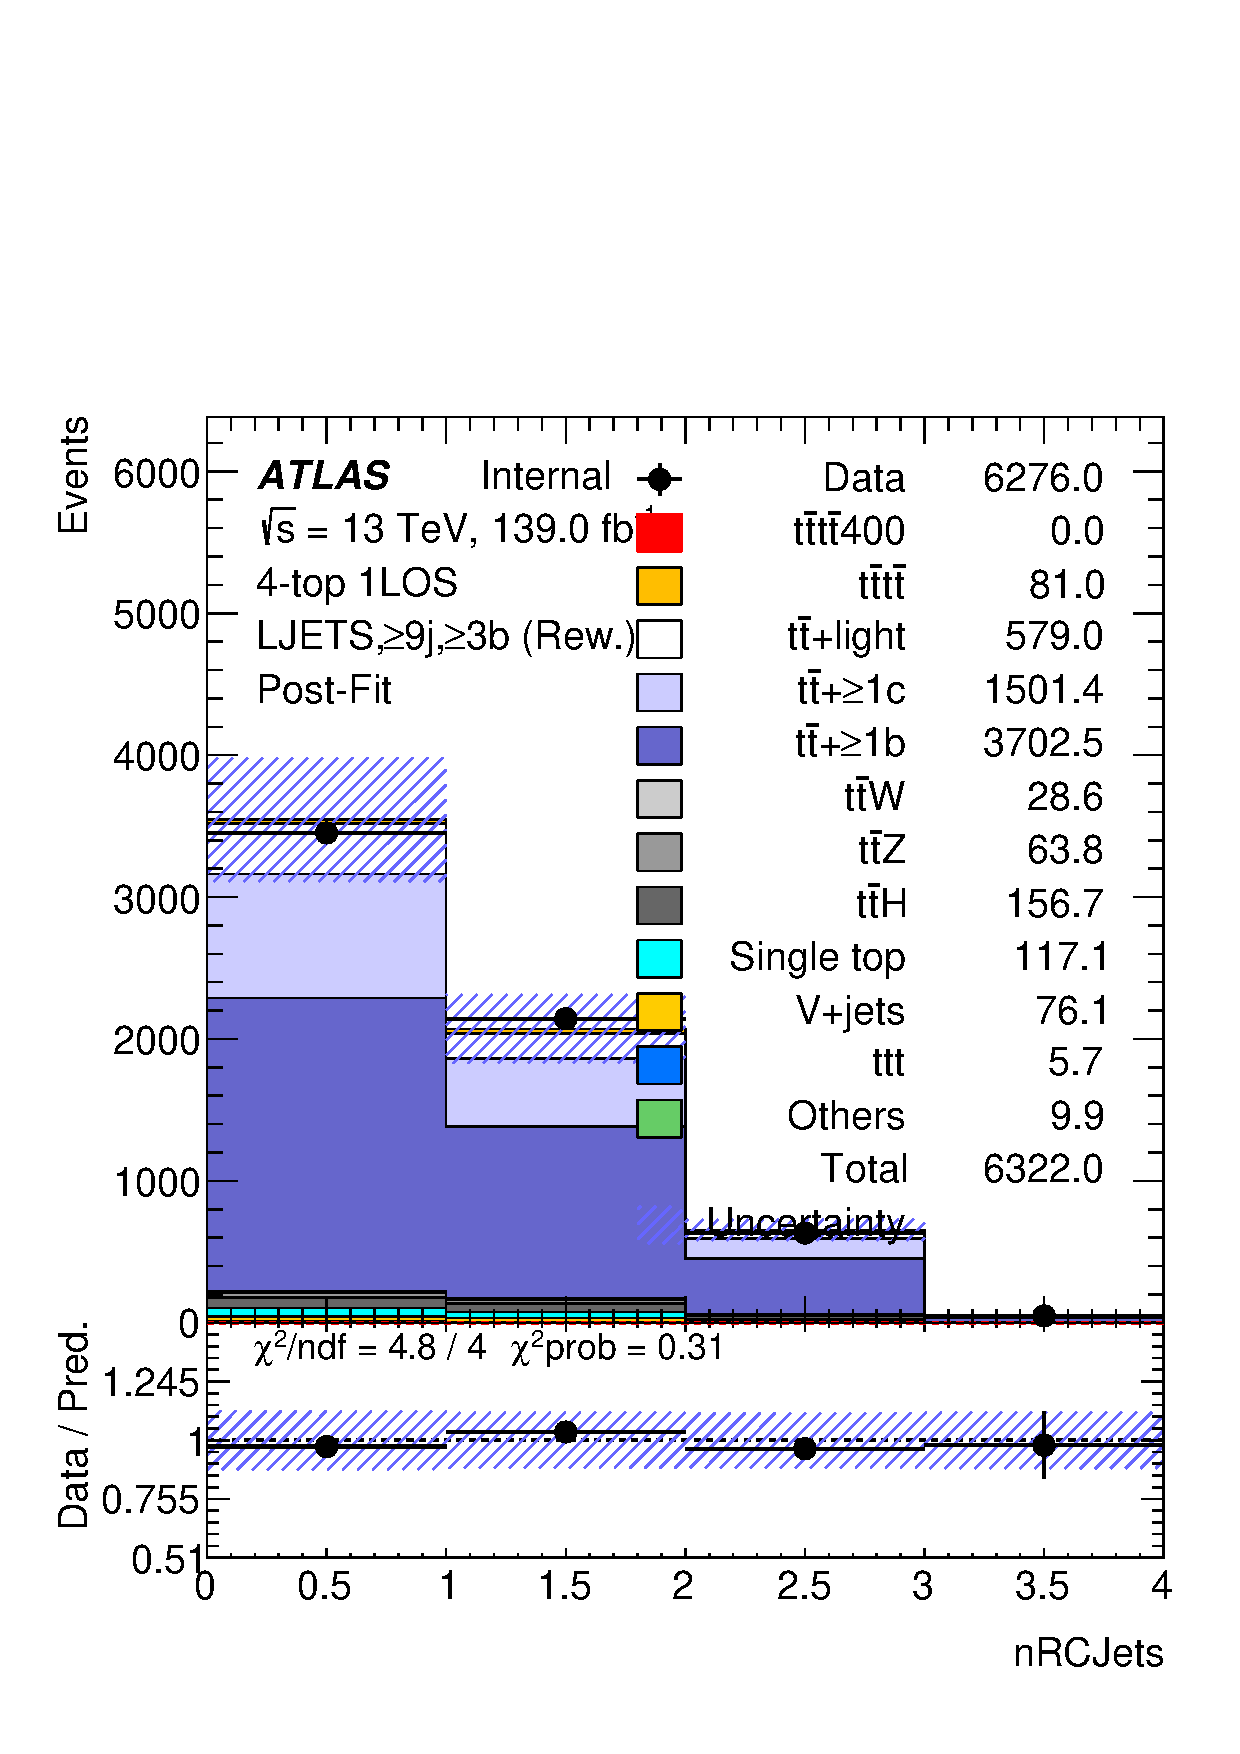
\includegraphics[width=0.3\textwidth]{figures/NNPlots/MVATrainRegion/Rew/ljets_ge9jge3b_nRCJetsM100_postFit.pdf}
    \caption{nRCJets}
    \end{center}
    \end{subfigure}

    \begin{subfigure}[t]{1\textwidth}
    \begin{center}
    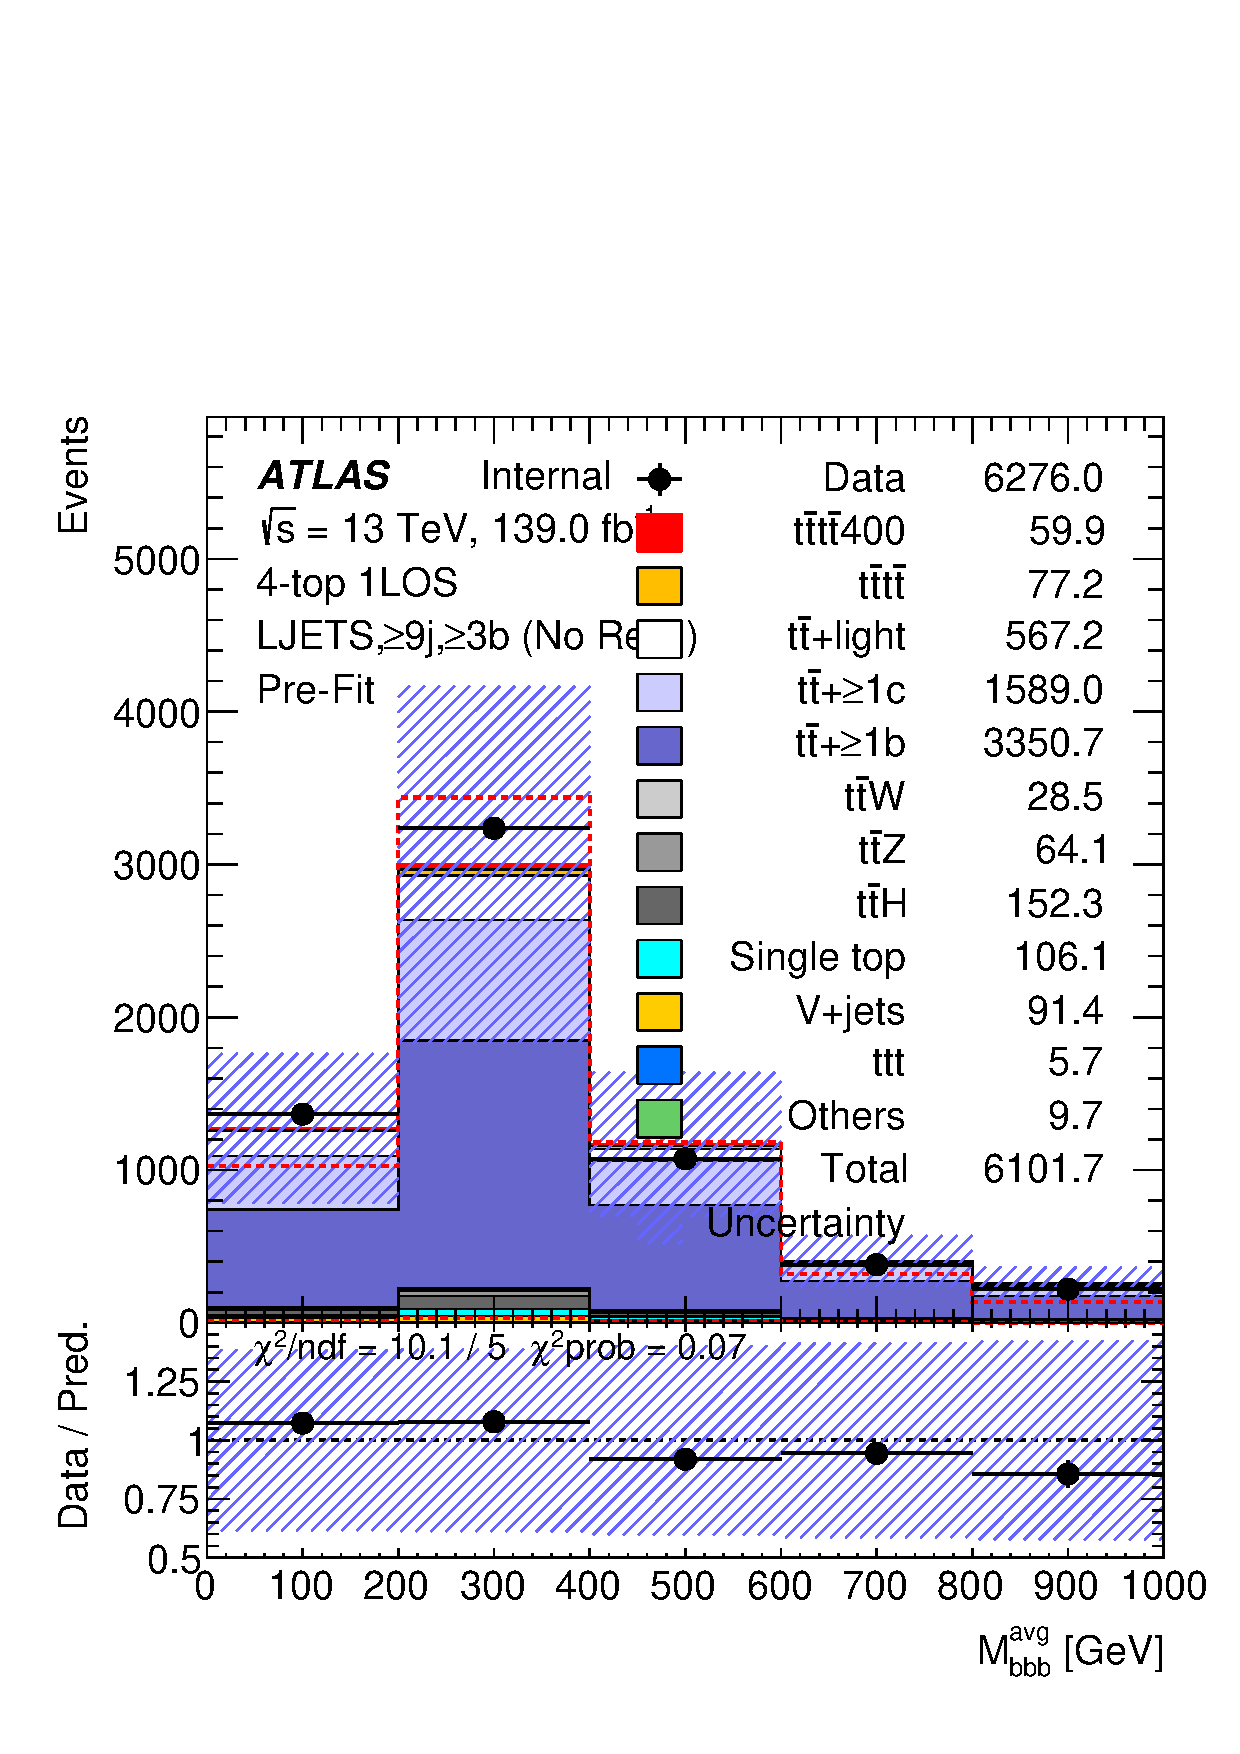
\includegraphics[width=0.3\textwidth]{figures/NNPlots/MVATrainRegion/NoRew/ljets_ge9jge3b_Mbbb_Avg_DL1r_70.pdf}
    
\includegraphics[width=0.3\textwidth]{figures/NNPlots/MVATrainRegion/Rew/ljets_ge9jge3b_Mbbb_Avg_DL1r_70.pdf}
    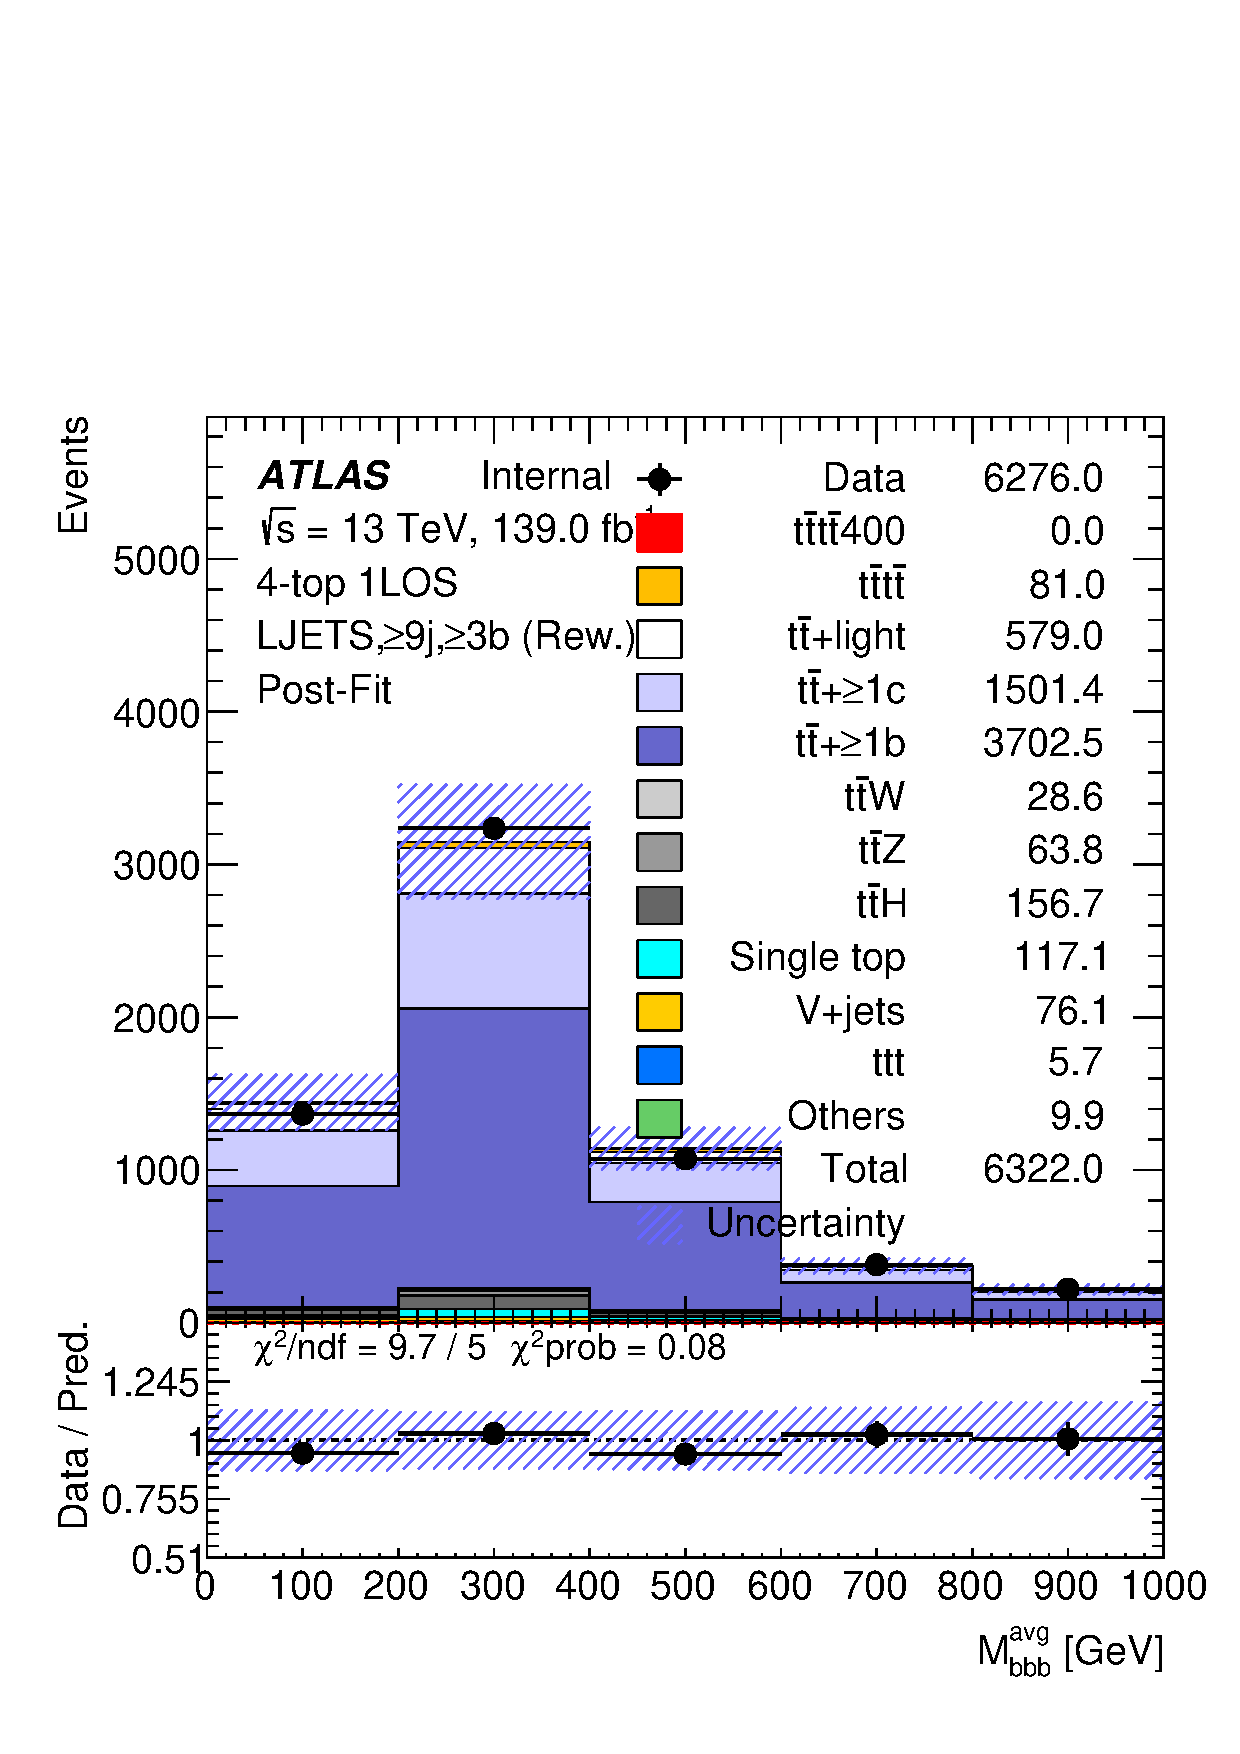
\includegraphics[width=0.3\textwidth]{figures/NNPlots/MVATrainRegion/Rew/ljets_ge9jge3b_Mbbb_Avg_DL1r_70_postFit.pdf}
    \caption{$M^{avg}_{bbb}$}
    \end{center}
    \end{subfigure}

    \begin{subfigure}[t]{1\textwidth}
    \begin{center}
    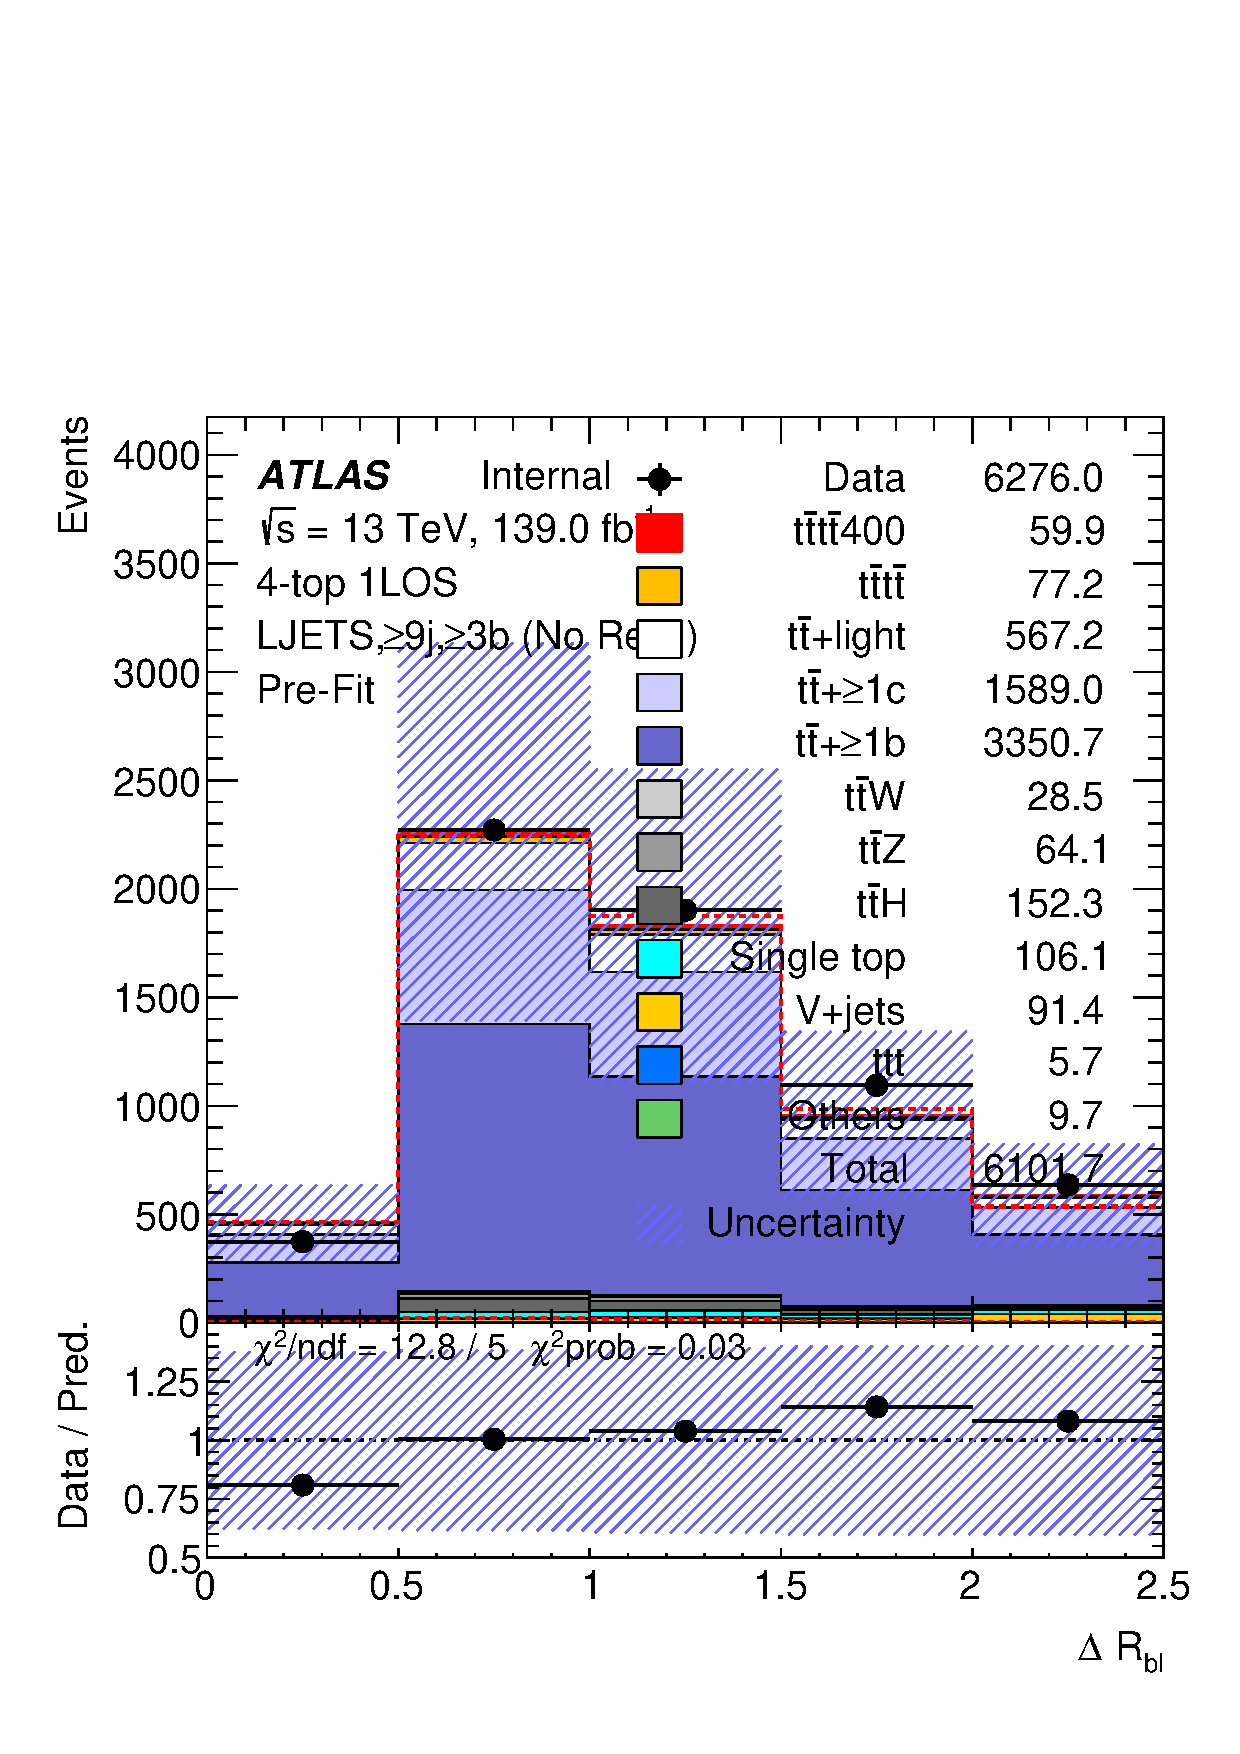
\includegraphics[width=0.3\textwidth]{figures/NNPlots/MVATrainRegion/NoRew/ljets_ge9jge3b_dRbl_MindR_DL1r_70.pdf}
    
\includegraphics[width=0.3\textwidth]{figures/NNPlots/MVATrainRegion/Rew/ljets_ge9jge3b_dRbl_MindR_DL1r_70.pdf}
    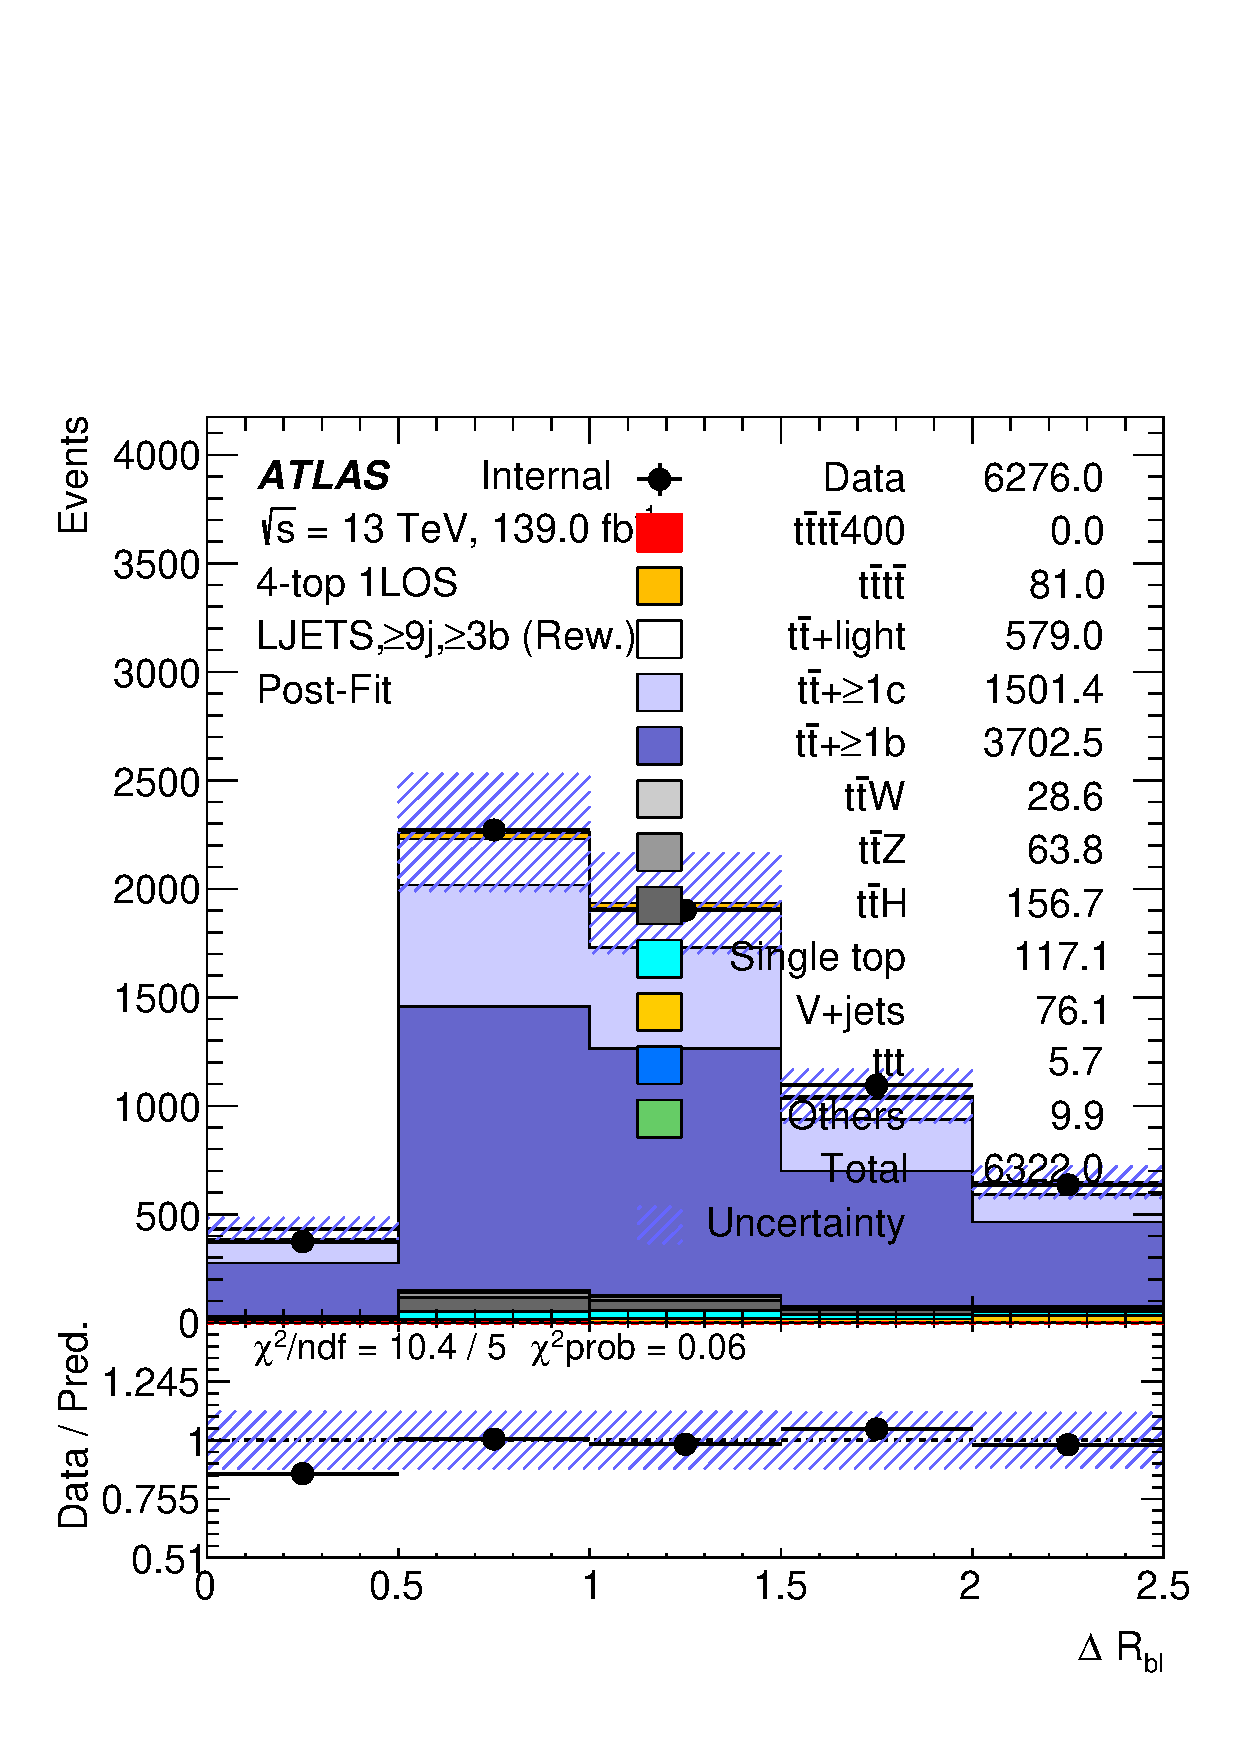
\includegraphics[width=0.3\textwidth]{figures/NNPlots/MVATrainRegion/Rew/ljets_ge9jge3b_dRbl_MindR_DL1r_70_postFit.pdf}
    \caption{$\Delta R^{min}_{bl}$}
    \end{center}
    \end{subfigure}
    \caption{\label{fig:NNPlots_MVATrainReg_3} The comparison between variables pre-fit distribution before (left) and after (middle) the NN-reweighting  in 1L MVA training regions ($\geq 9j,\geq 3b$). The post-fit distribution after the NN-reweighting is shown on the left. Blinded regions are excluded.}
\end{figure}

\begin{figure}[htbp!]
    \begin{subfigure}[t]{1\textwidth}
    \begin{center}
    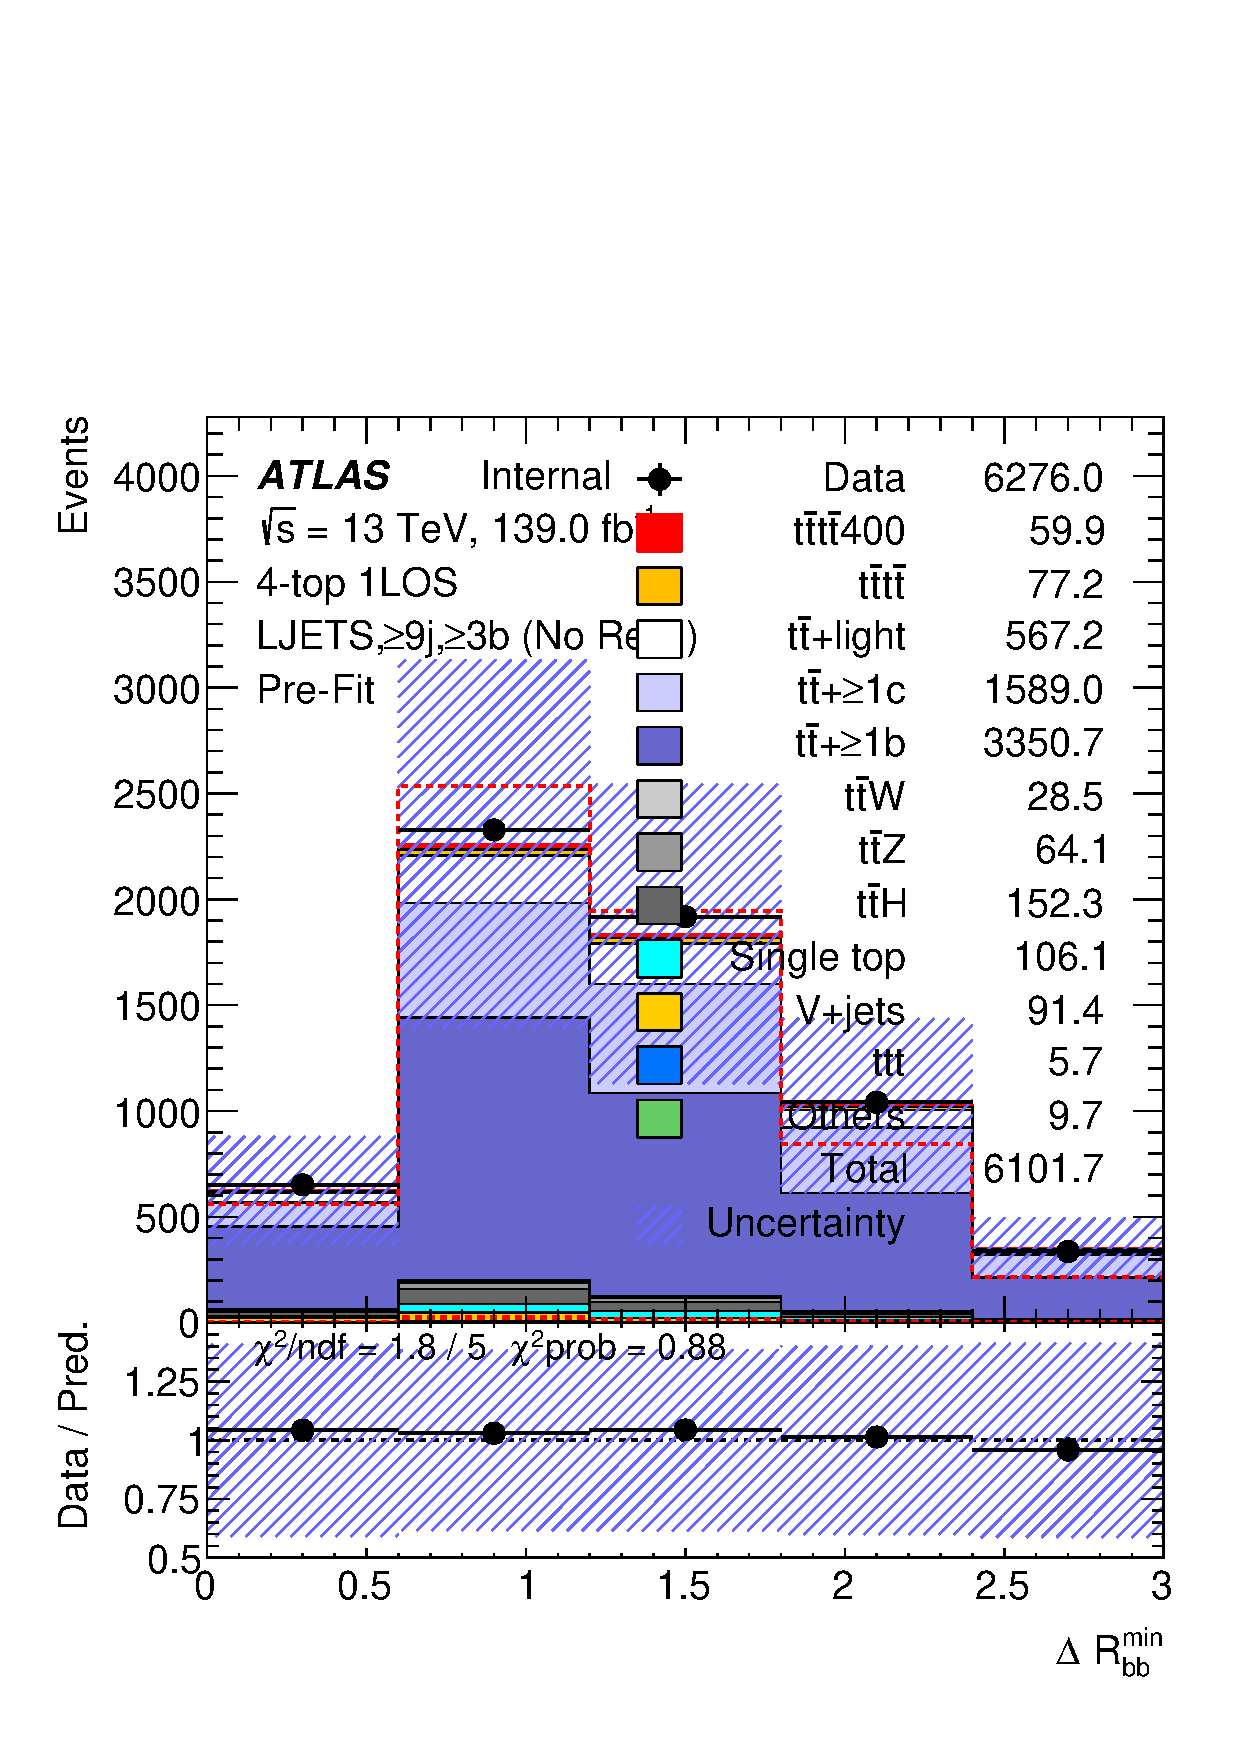
\includegraphics[width=0.3\textwidth]{figures/NNPlots/MVATrainRegion/NoRew/ljets_ge9jge3b_dRbb_MindR_DL1r_70.pdf}
    
\includegraphics[width=0.3\textwidth]{figures/NNPlots/MVATrainRegion/Rew/ljets_ge9jge3b_dRbb_MindR_DL1r_70.pdf}
    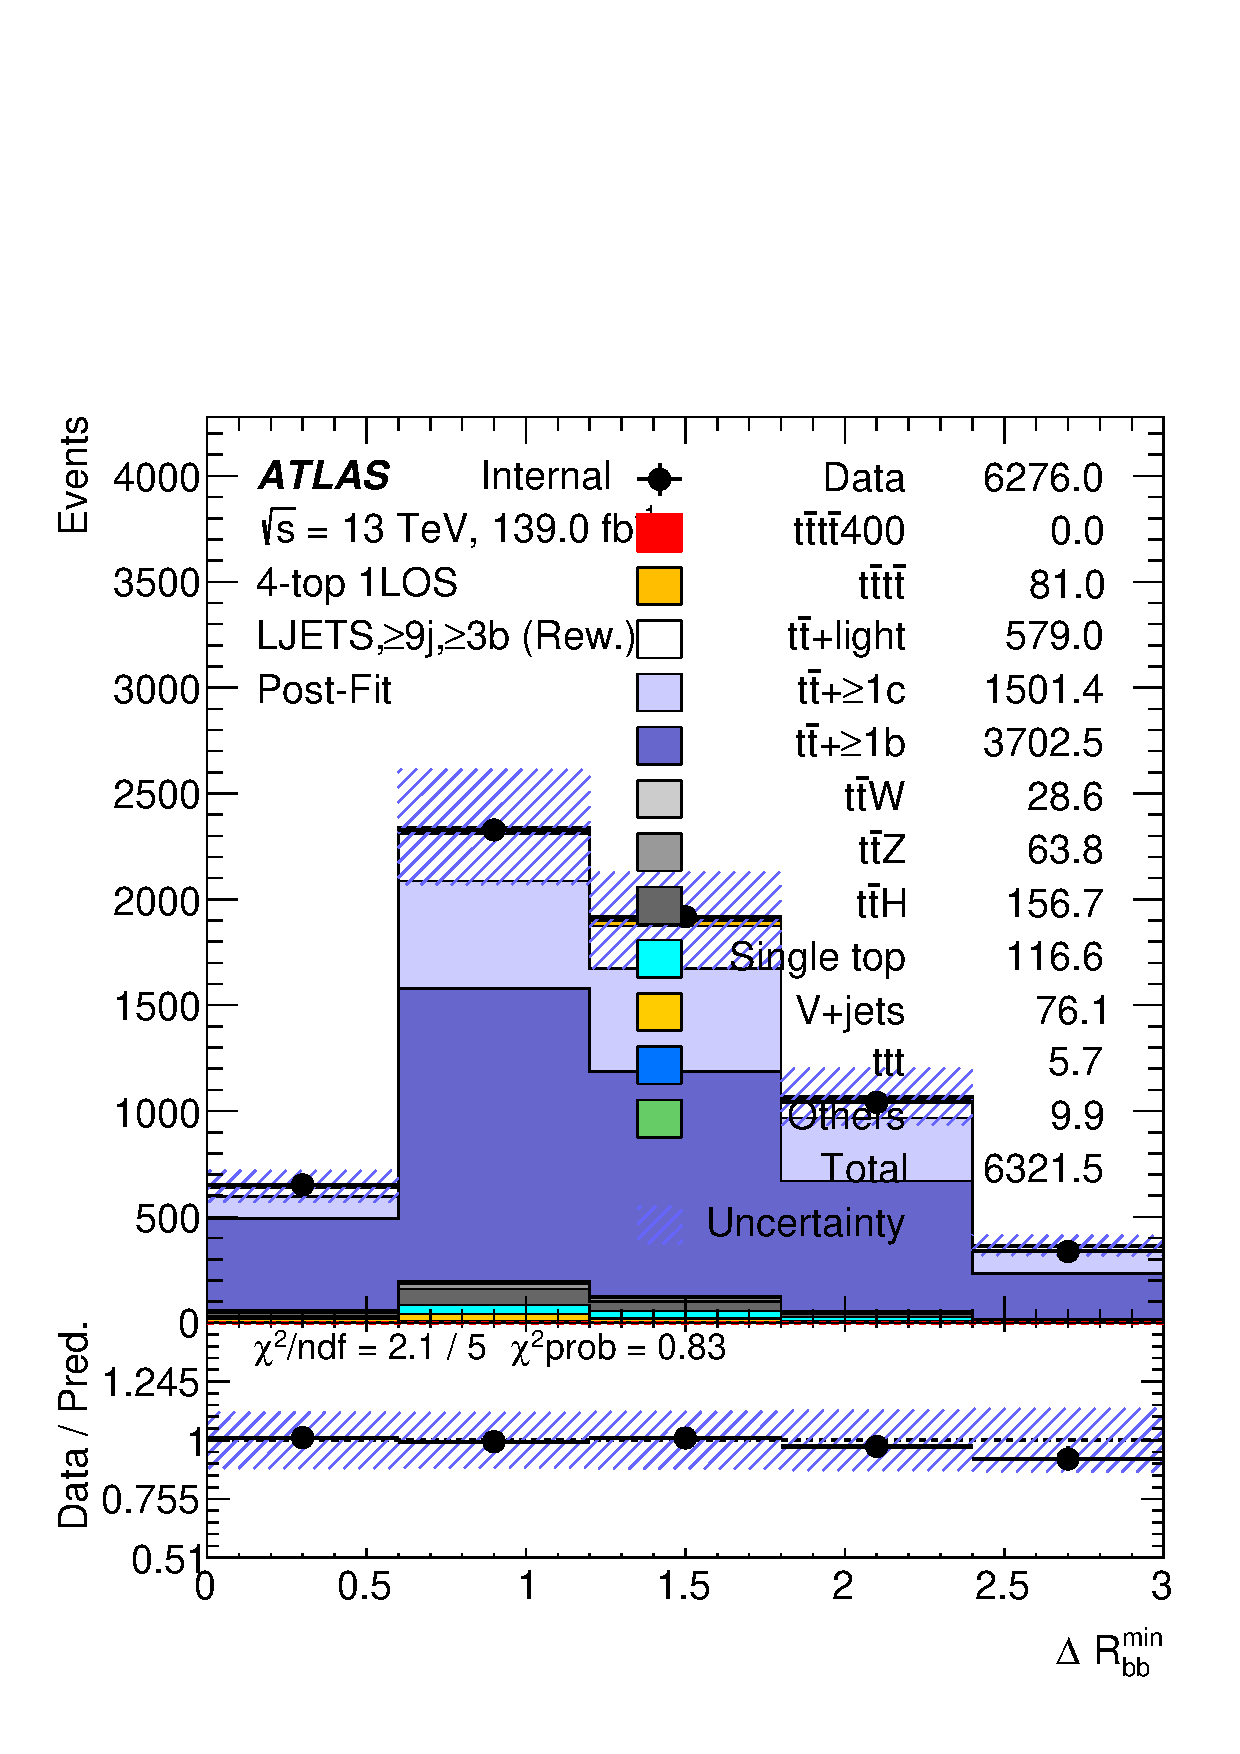
\includegraphics[width=0.3\textwidth]{figures/NNPlots/MVATrainRegion/Rew/ljets_ge9jge3b_dRbb_MindR_DL1r_70_postFit.pdf}
    \caption{$\Delta R^{min}_{bb}$}
    \end{center}
    \end{subfigure}

    \begin{subfigure}[t]{1\textwidth}
    \begin{center}
    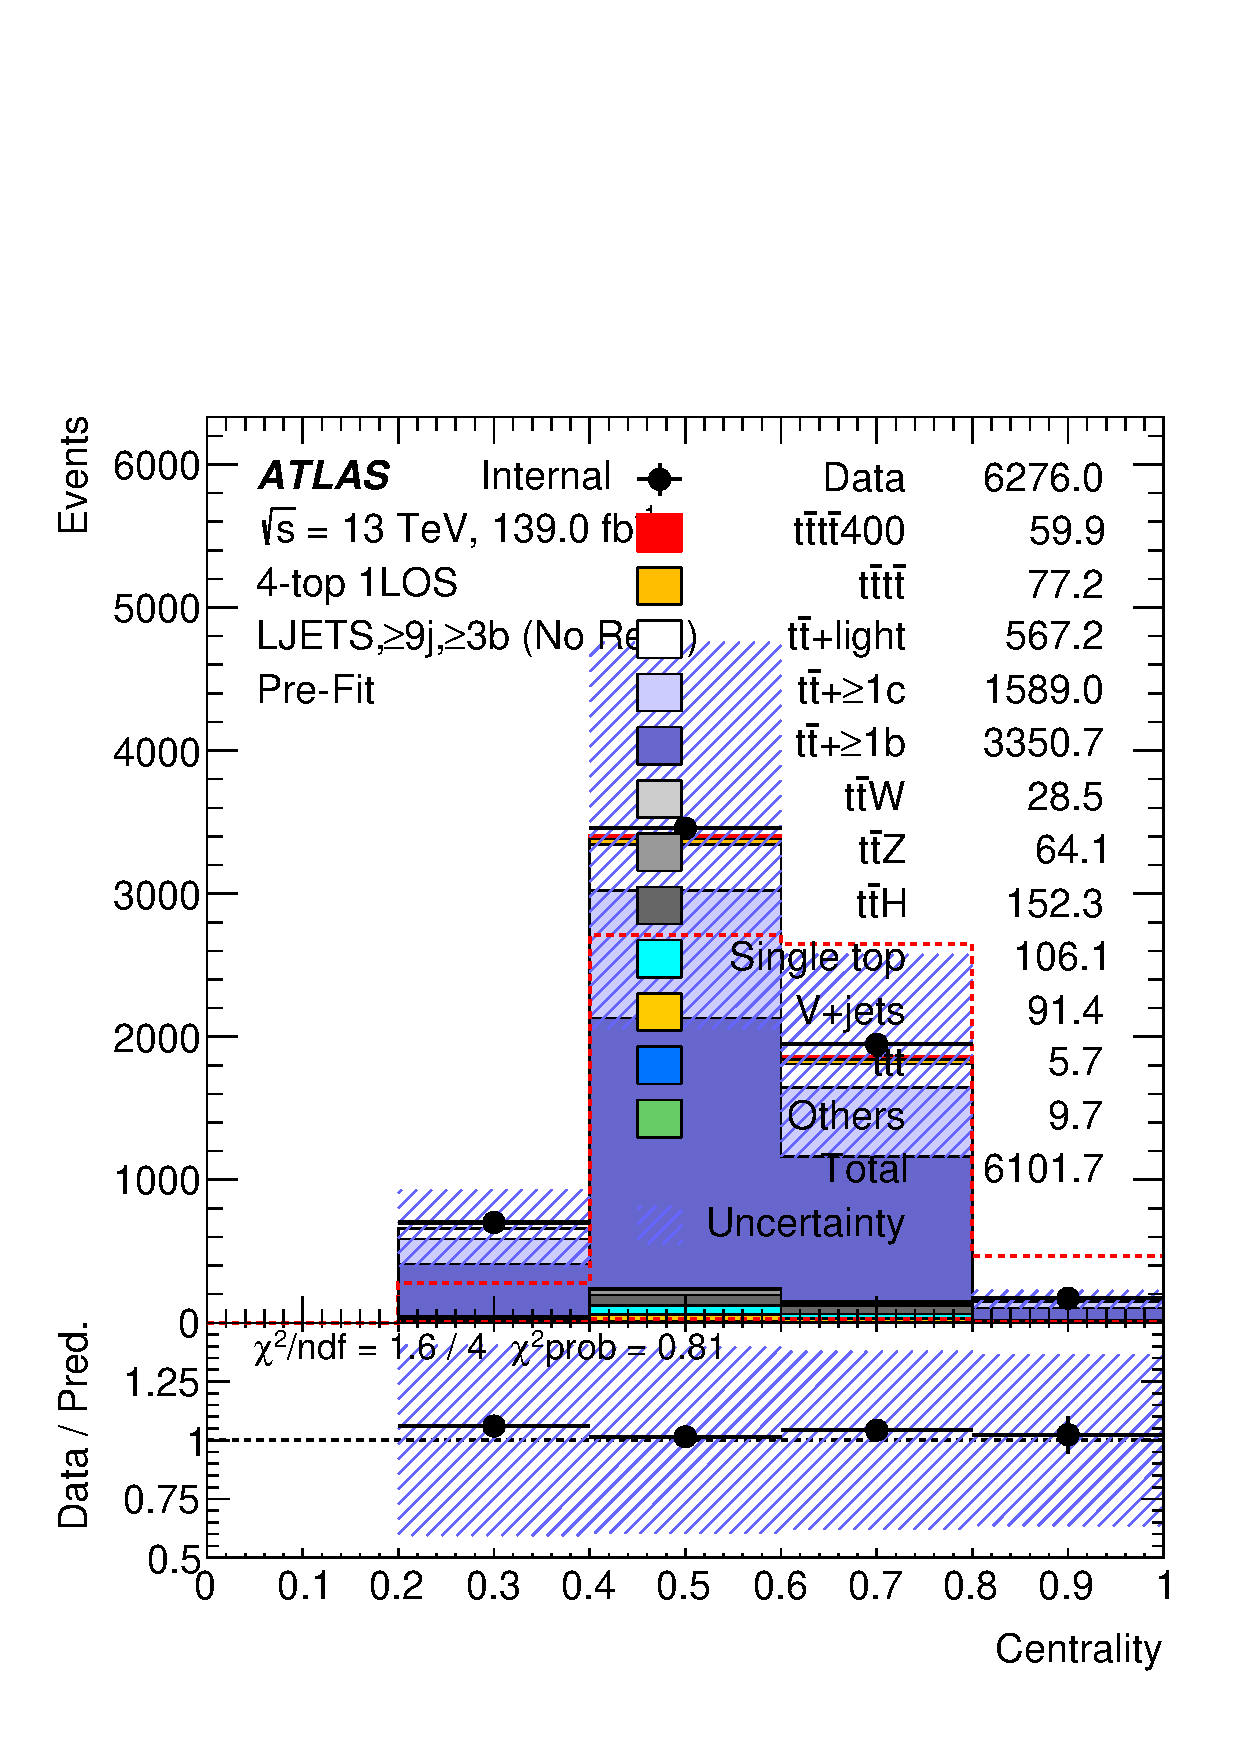
\includegraphics[width=0.3\textwidth]{figures/NNPlots/MVATrainRegion/NoRew/ljets_ge9jge3b_Centrality_all.pdf}
    
\includegraphics[width=0.3\textwidth]{figures/NNPlots/MVATrainRegion/Rew/ljets_ge9jge3b_Centrality_all.pdf}
    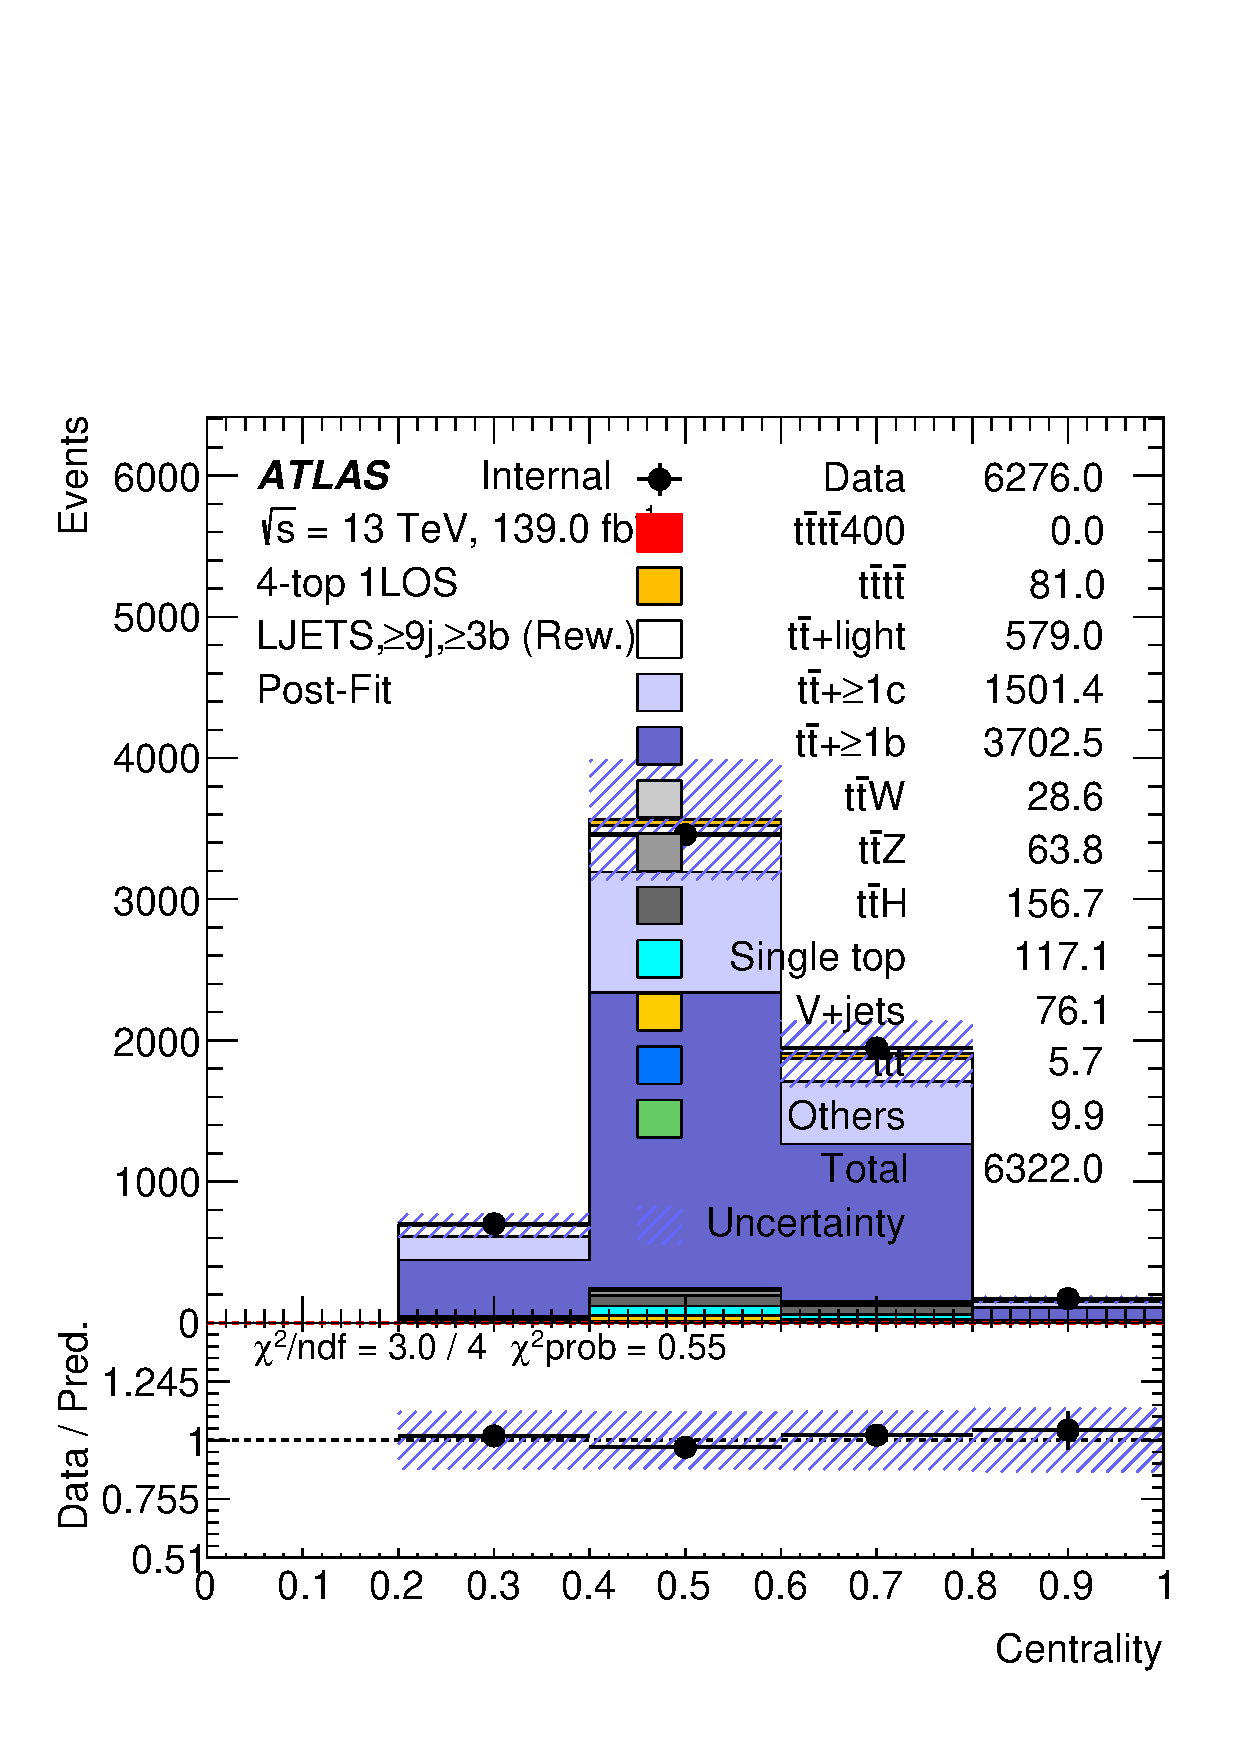
\includegraphics[width=0.3\textwidth]{figures/NNPlots/MVATrainRegion/Rew/ljets_ge9jge3b_Centrality_all_postFit.pdf}
    \caption{Centrality}
    \end{center}
    \end{subfigure}

    \begin{subfigure}[t]{1\textwidth}
    \begin{center}
    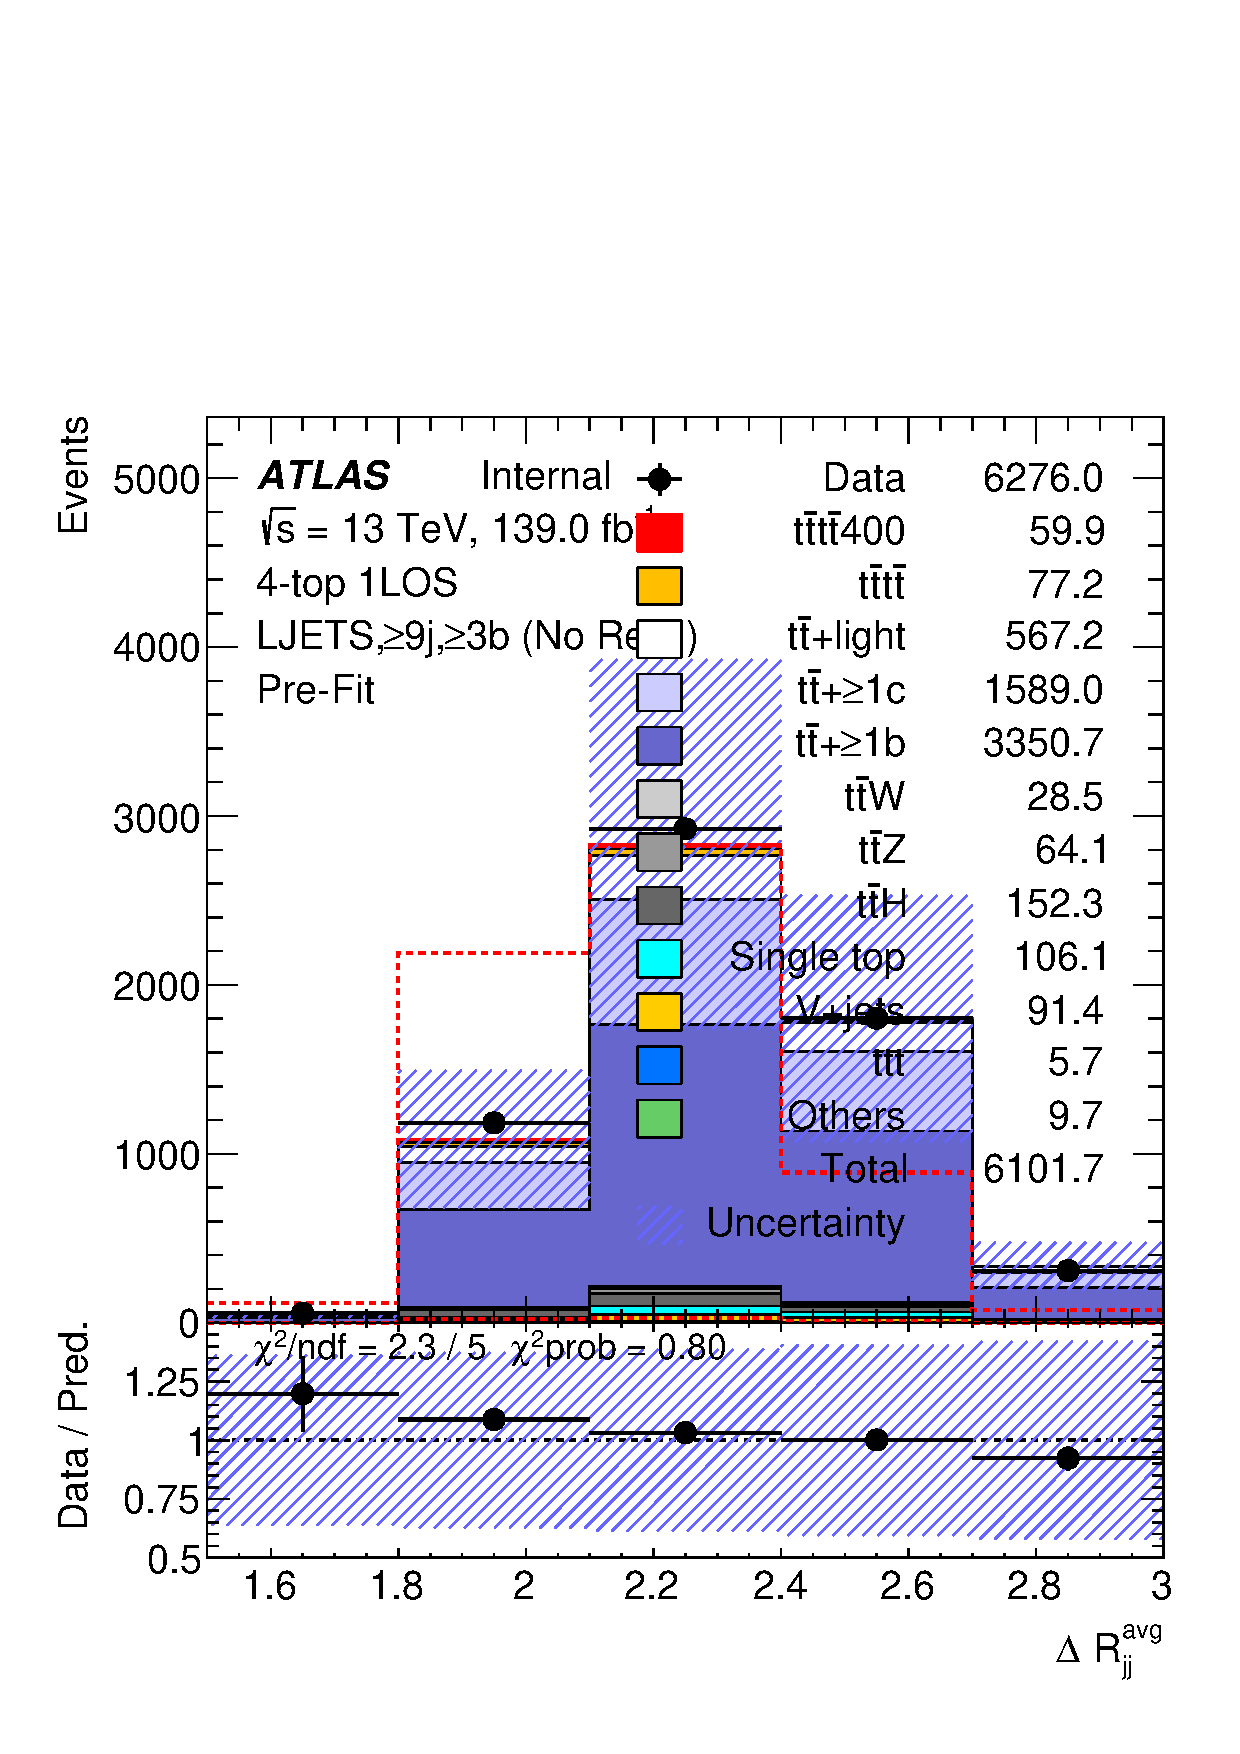
\includegraphics[width=0.3\textwidth]{figures/NNPlots/MVATrainRegion/NoRew/ljets_ge9jge3b_dRjj_Avg.pdf}
    
\includegraphics[width=0.3\textwidth]{figures/NNPlots/MVATrainRegion/Rew/ljets_ge9jge3b_dRjj_Avg.pdf}
    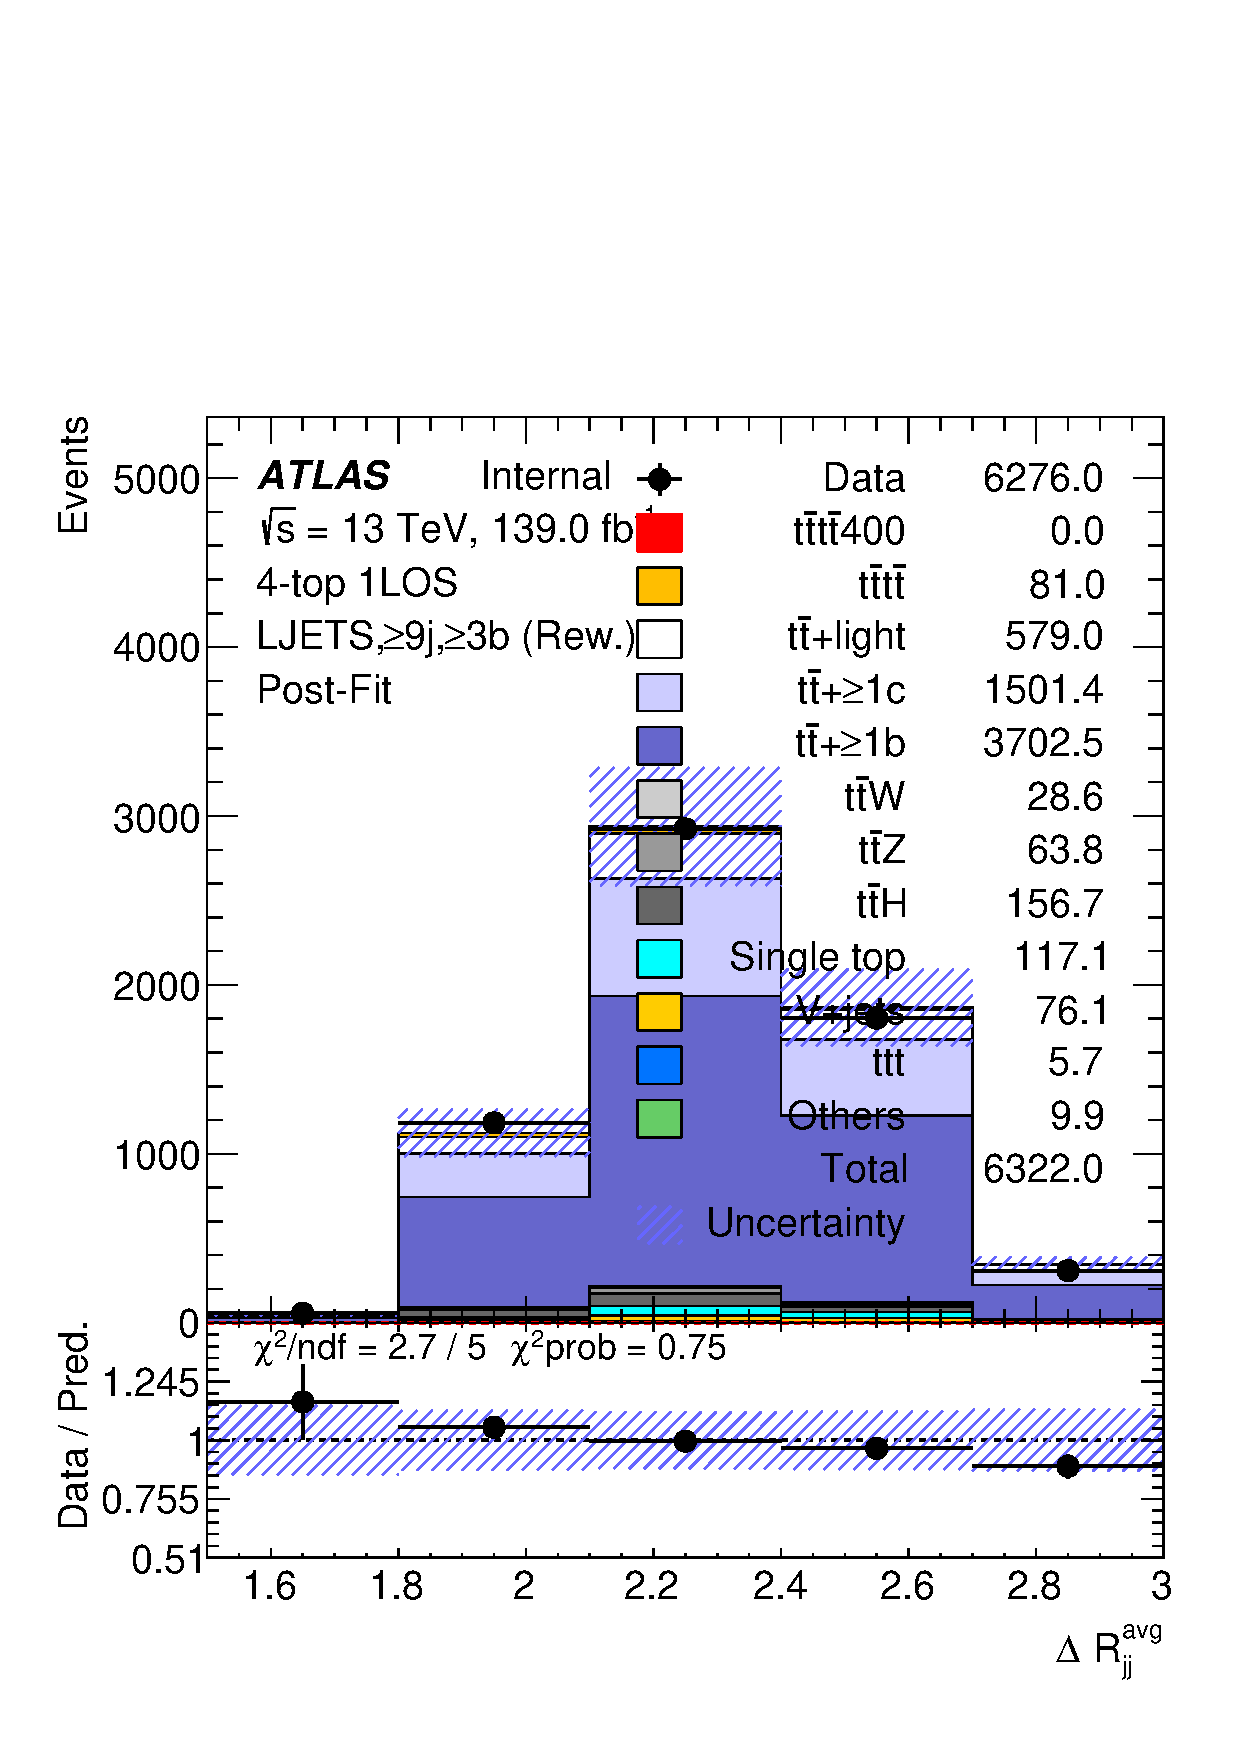
\includegraphics[width=0.3\textwidth]{figures/NNPlots/MVATrainRegion/Rew/ljets_ge9jge3b_dRjj_Avg_postFit.pdf}
    \caption{$\Delta R^{avg}_{jj}$}
    \end{center}
    \end{subfigure}
    \caption{\label{fig:NNPlots_MVATrainReg_4} The comparison between variables pre-fit distribution before (left) and after (middle) the NN-reweighting  in 1L MVA training regions ($\geq 9j,\geq 3b$). The post-fit distribution after the NN-reweighting is shown on the left. Blinded regions are excluded.}
\end{figure}

\begin{figure}[htbp!]
    \begin{subfigure}[t]{1\textwidth}
    \begin{center}
    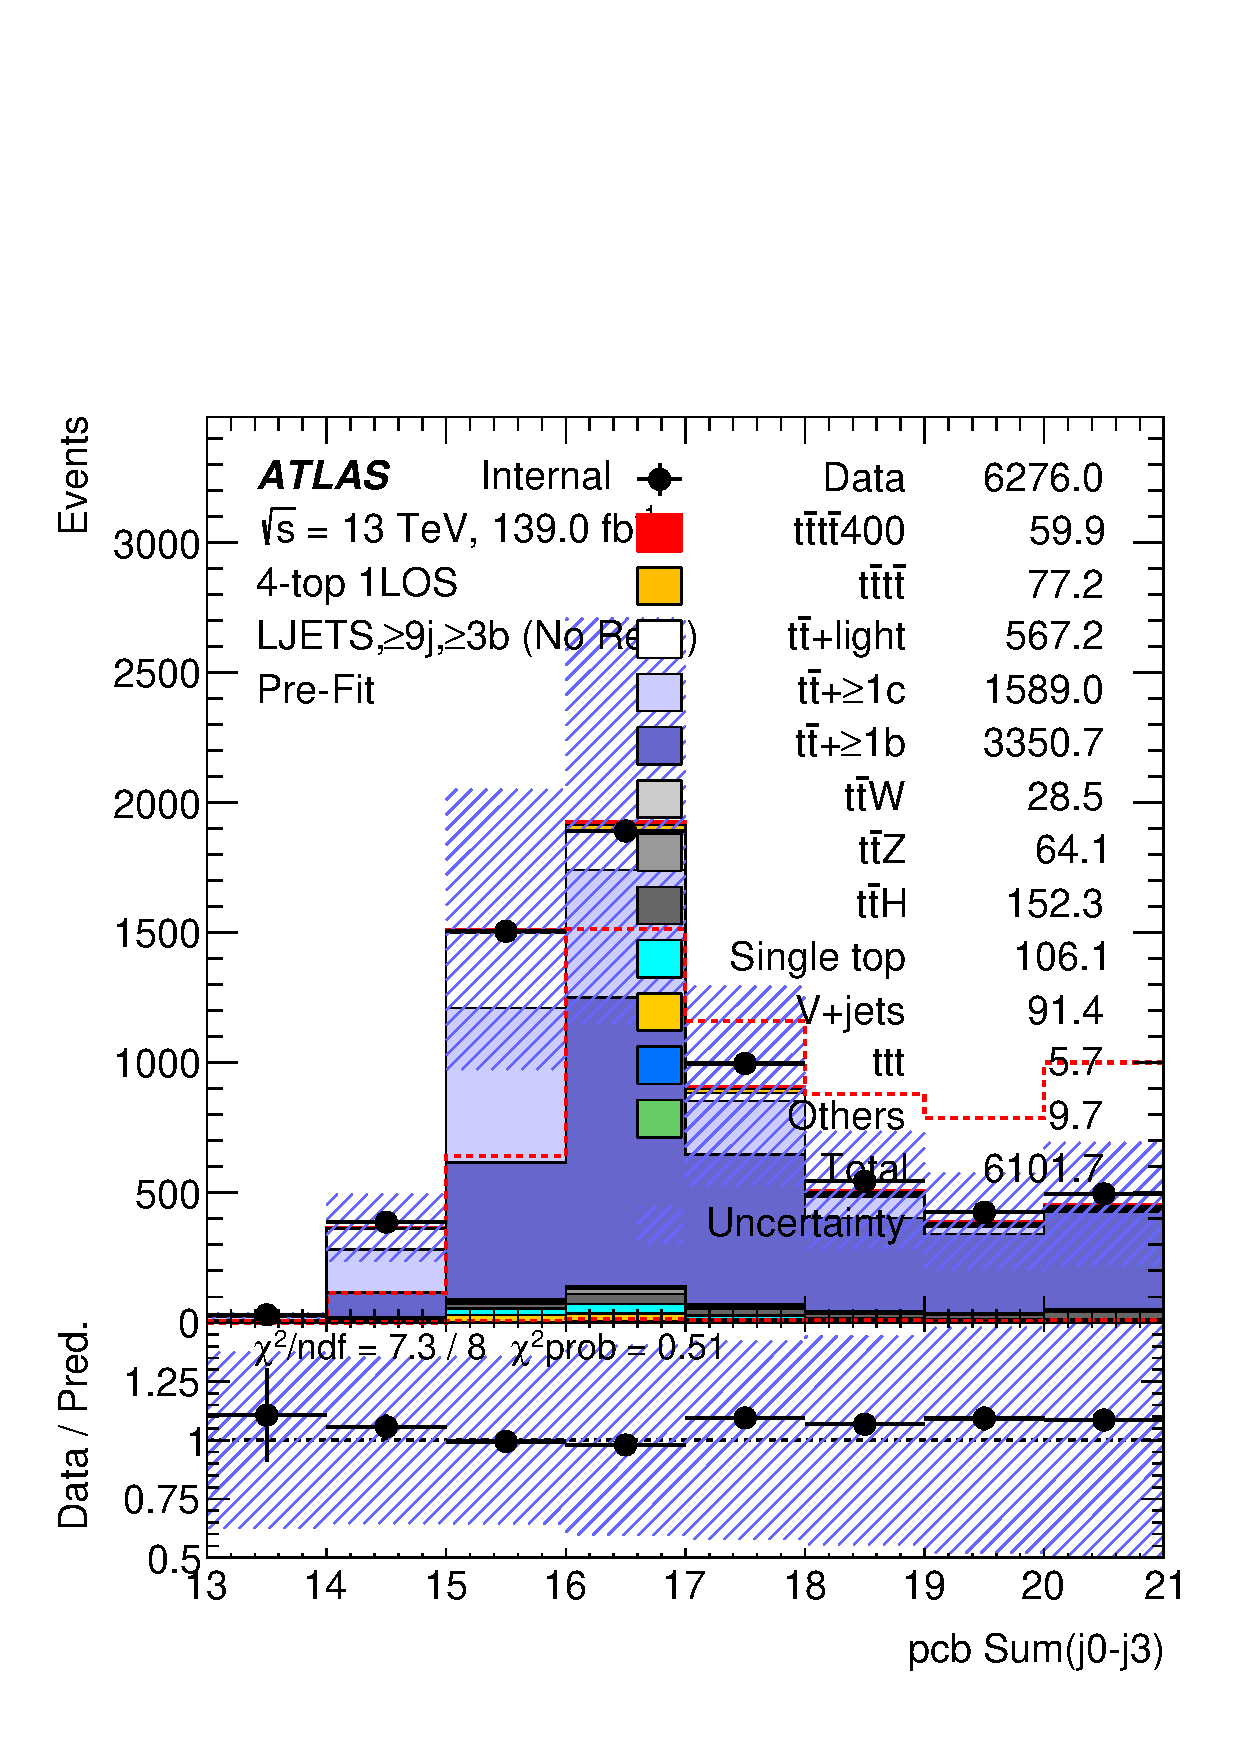
\includegraphics[width=0.3\textwidth]{figures/NNPlots/MVATrainRegion/NoRew/ljets_ge9jge3b_pcb.pdf}
    
\includegraphics[width=0.3\textwidth]{figures/NNPlots/MVATrainRegion/Rew/ljets_ge9jge3b_pcb.pdf}
    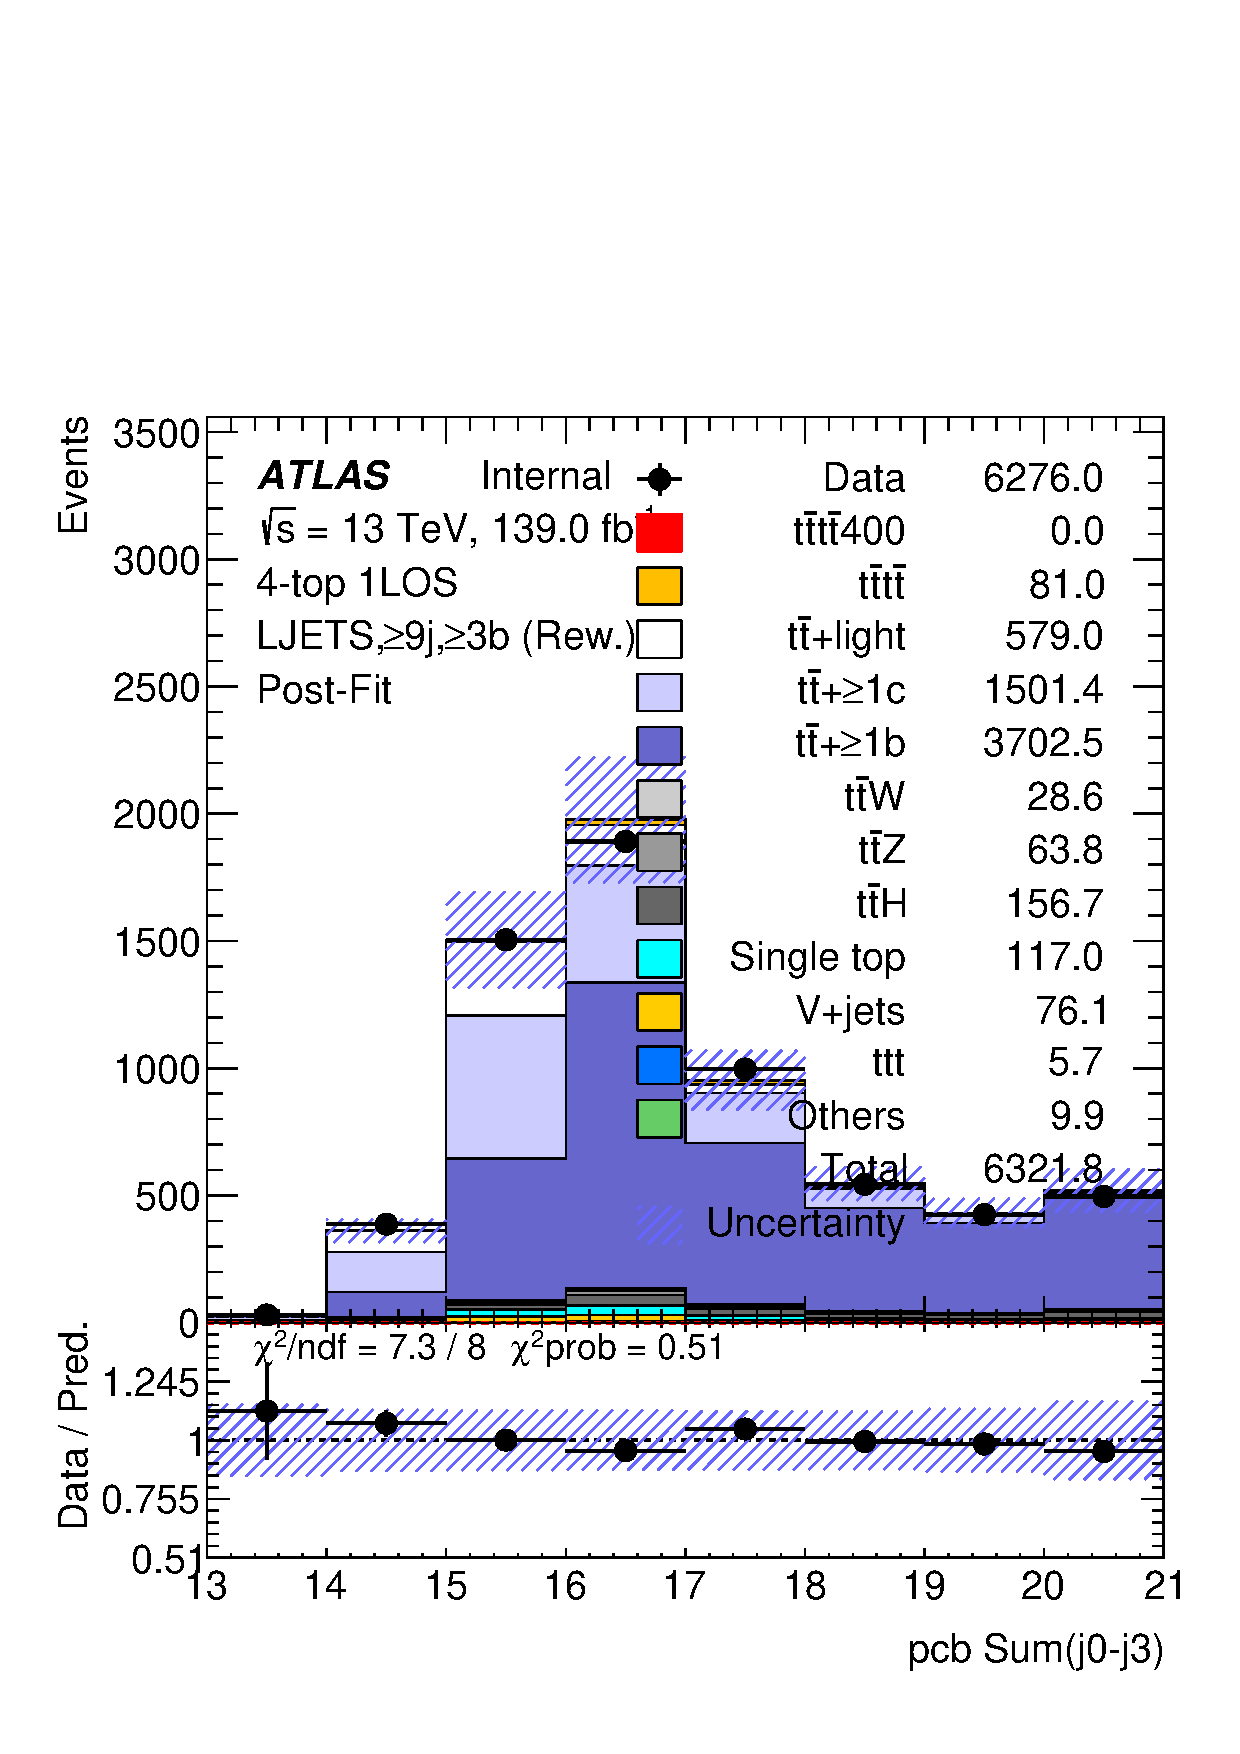
\includegraphics[width=0.3\textwidth]{figures/NNPlots/MVATrainRegion/Rew/ljets_ge9jge3b_pcb_postFit.pdf}
    \caption{pcb Sum}
    \end{center}
    \end{subfigure}

    \begin{subfigure}[t]{1\textwidth}
    \begin{center}
    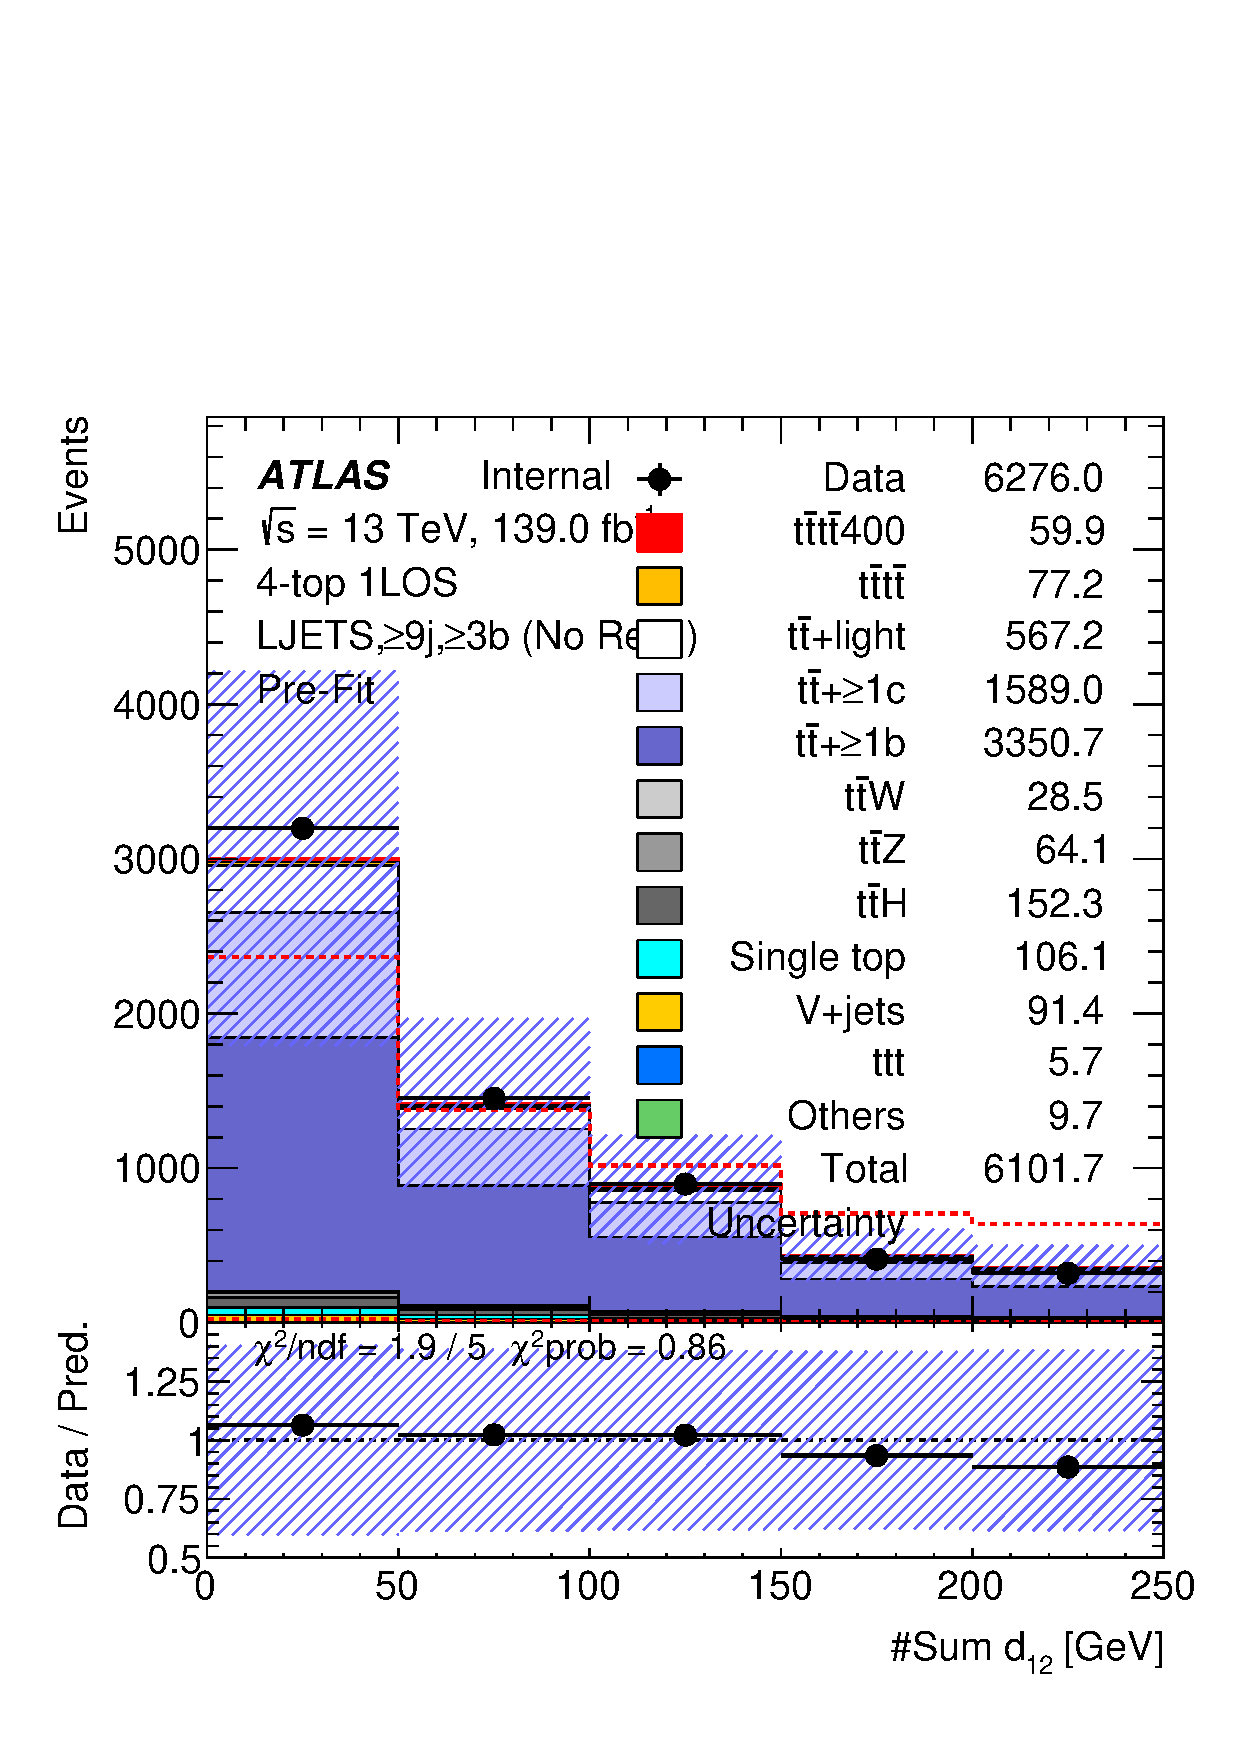
\includegraphics[width=0.3\textwidth]{figures/NNPlots/MVATrainRegion/NoRew/ljets_ge9jge3b_sum_d12.pdf}
    
\includegraphics[width=0.3\textwidth]{figures/NNPlots/MVATrainRegion/Rew/ljets_ge9jge3b_sum_d12.pdf}
    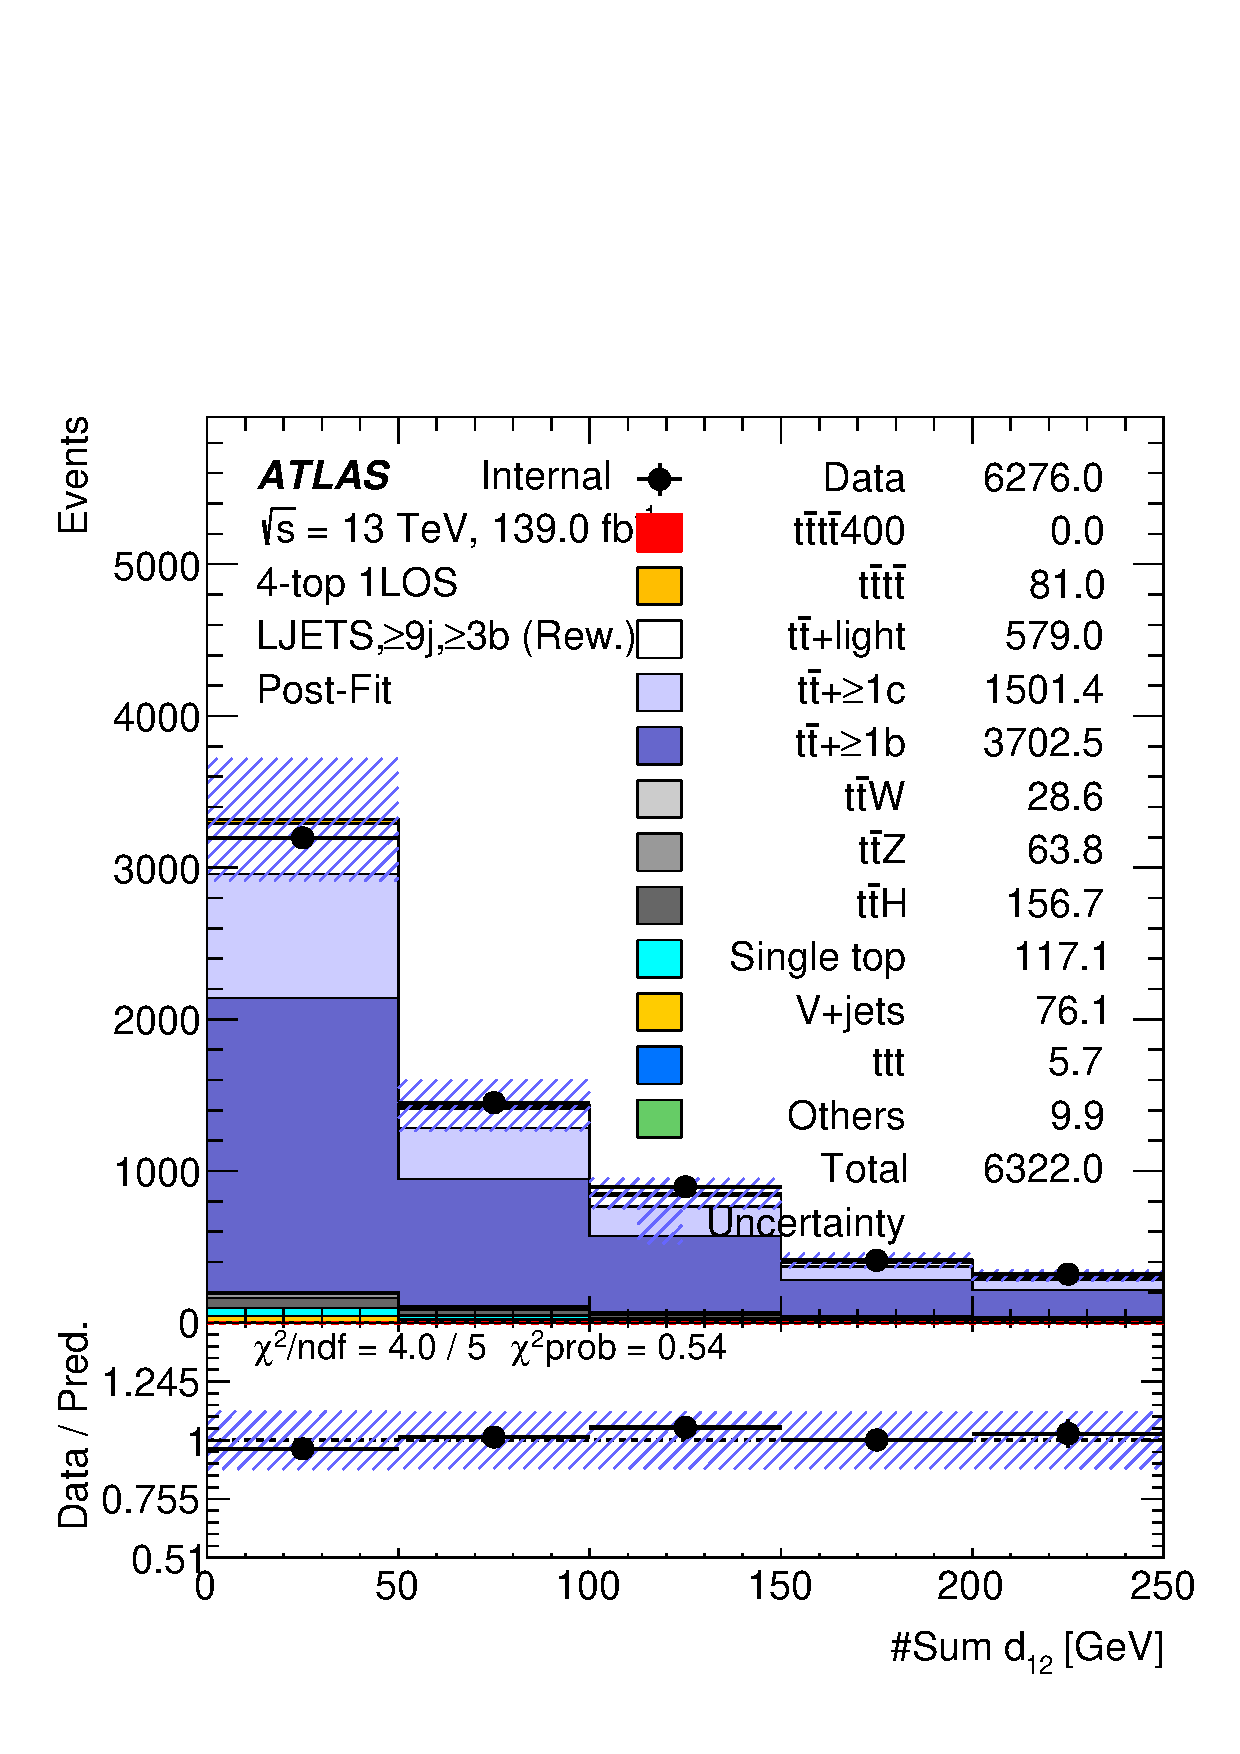
\includegraphics[width=0.3\textwidth]{figures/NNPlots/MVATrainRegion/Rew/ljets_ge9jge3b_sum_d12_postFit.pdf}
    \caption{$\sum d_{12}$}
    \end{center}
    \end{subfigure}

    \begin{subfigure}[t]{1\textwidth}
    \begin{center}
    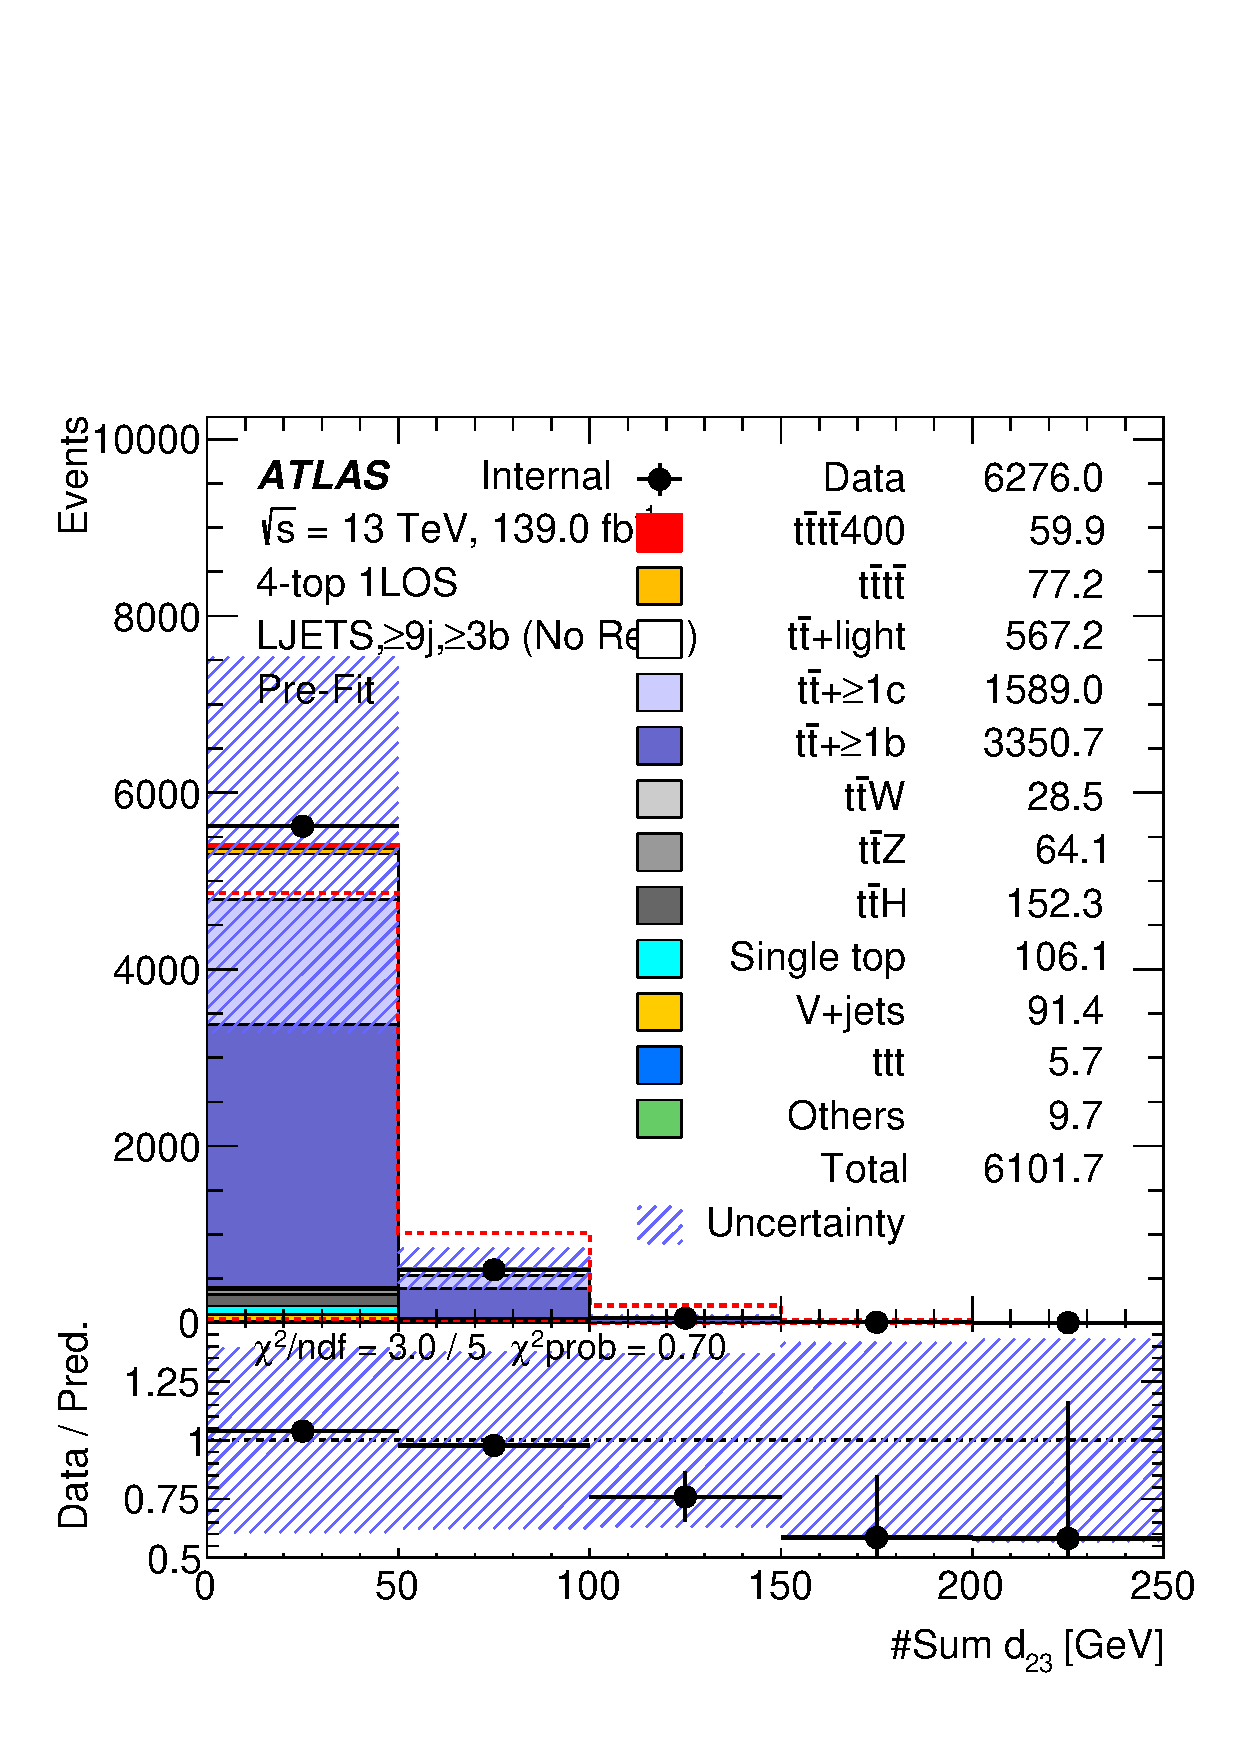
\includegraphics[width=0.3\textwidth]{figures/NNPlots/MVATrainRegion/NoRew/ljets_ge9jge3b_sum_d23.pdf}
    
\includegraphics[width=0.3\textwidth]{figures/NNPlots/MVATrainRegion/Rew/ljets_ge9jge3b_sum_d23.pdf}
    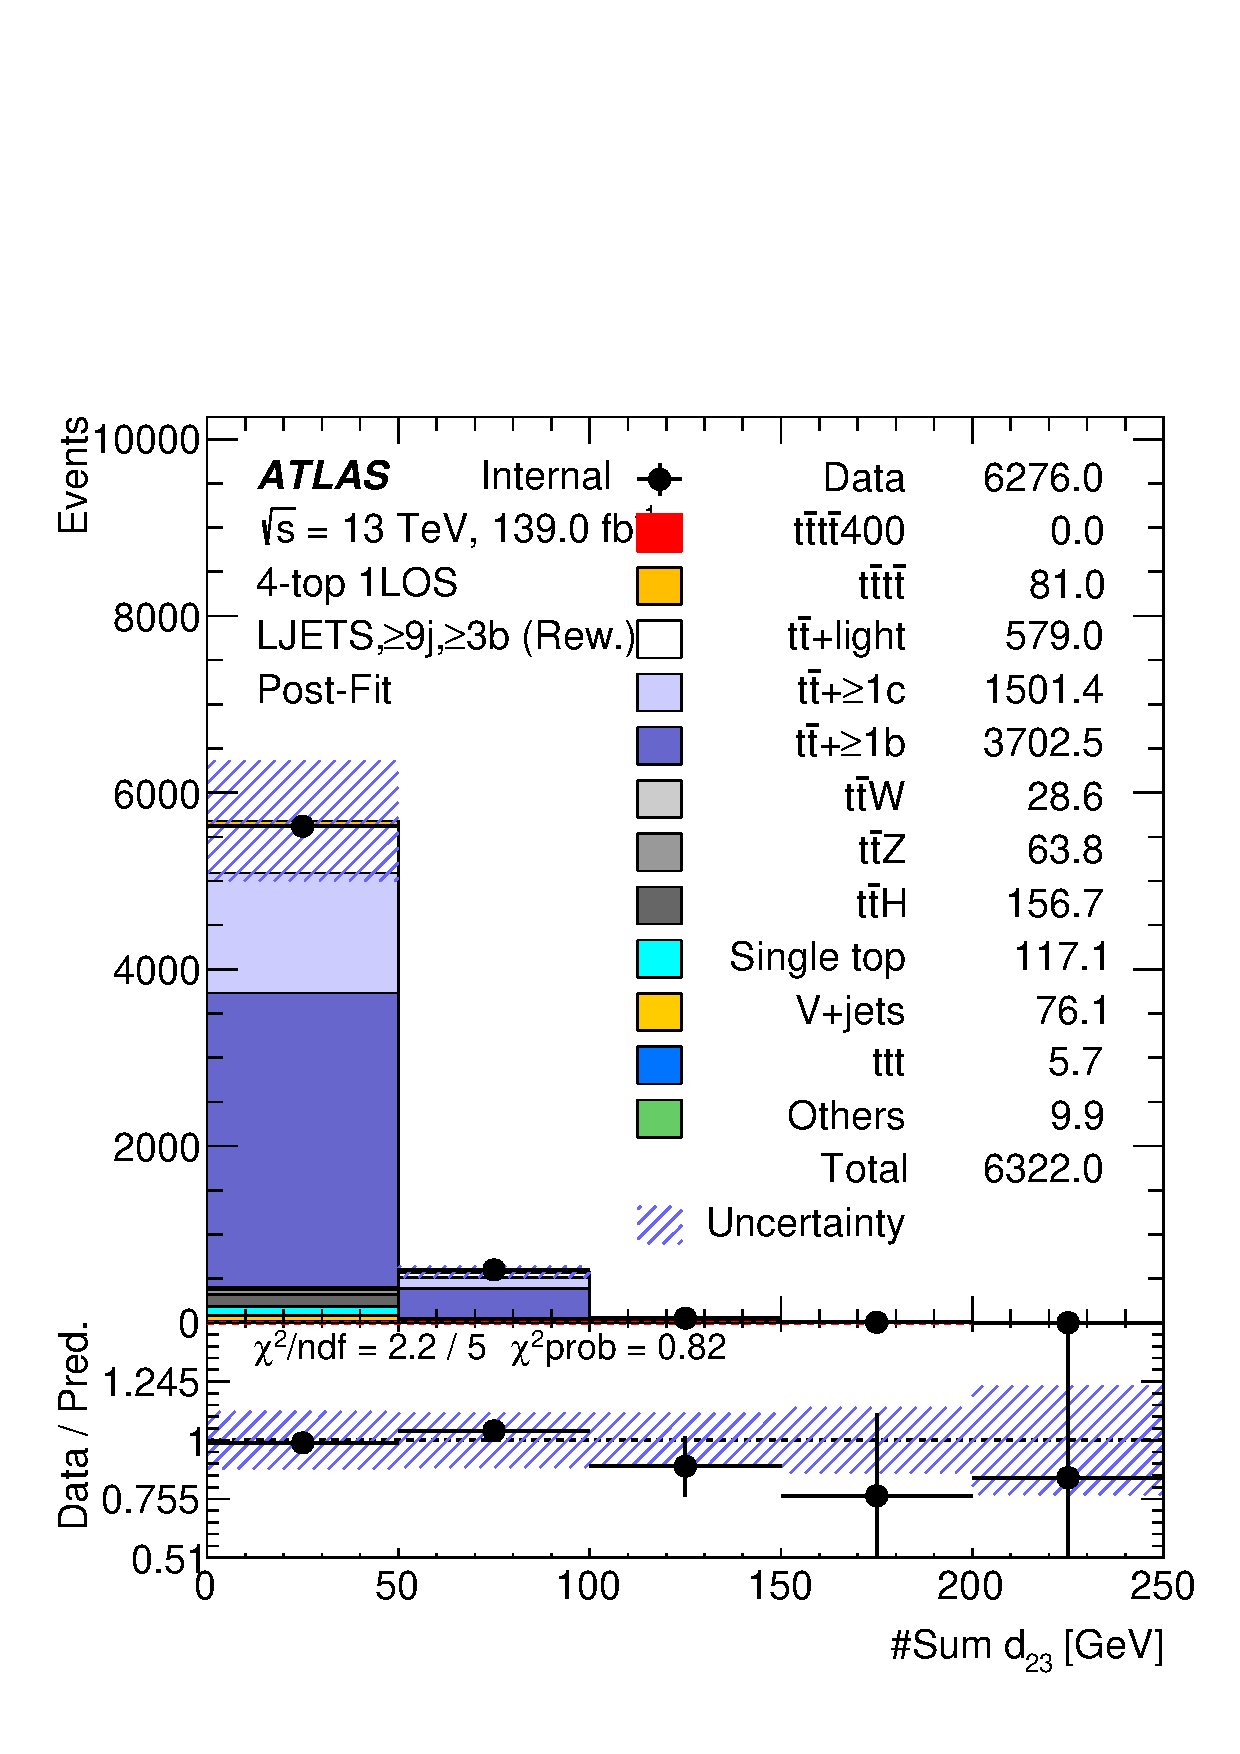
\includegraphics[width=0.3\textwidth]{figures/NNPlots/MVATrainRegion/Rew/ljets_ge9jge3b_sum_d23_postFit.pdf}
    \caption{$\sum d_{23}$}
    \end{center}
    \end{subfigure}
    \caption{\label{fig:NNPlots_MVATrainReg_5} The comparison between variables pre-fit distribution before (left) and after (middle) the NN-reweighting  in 1L MVA training regions ($\geq 9j,\geq 3b$). The post-fit distribution after the NN-reweighting is shown on the left. Blinded regions are excluded.}
\end{figure}

\begin{figure}[htbp!]
    \begin{subfigure}[t]{1\textwidth}
    \begin{center}
    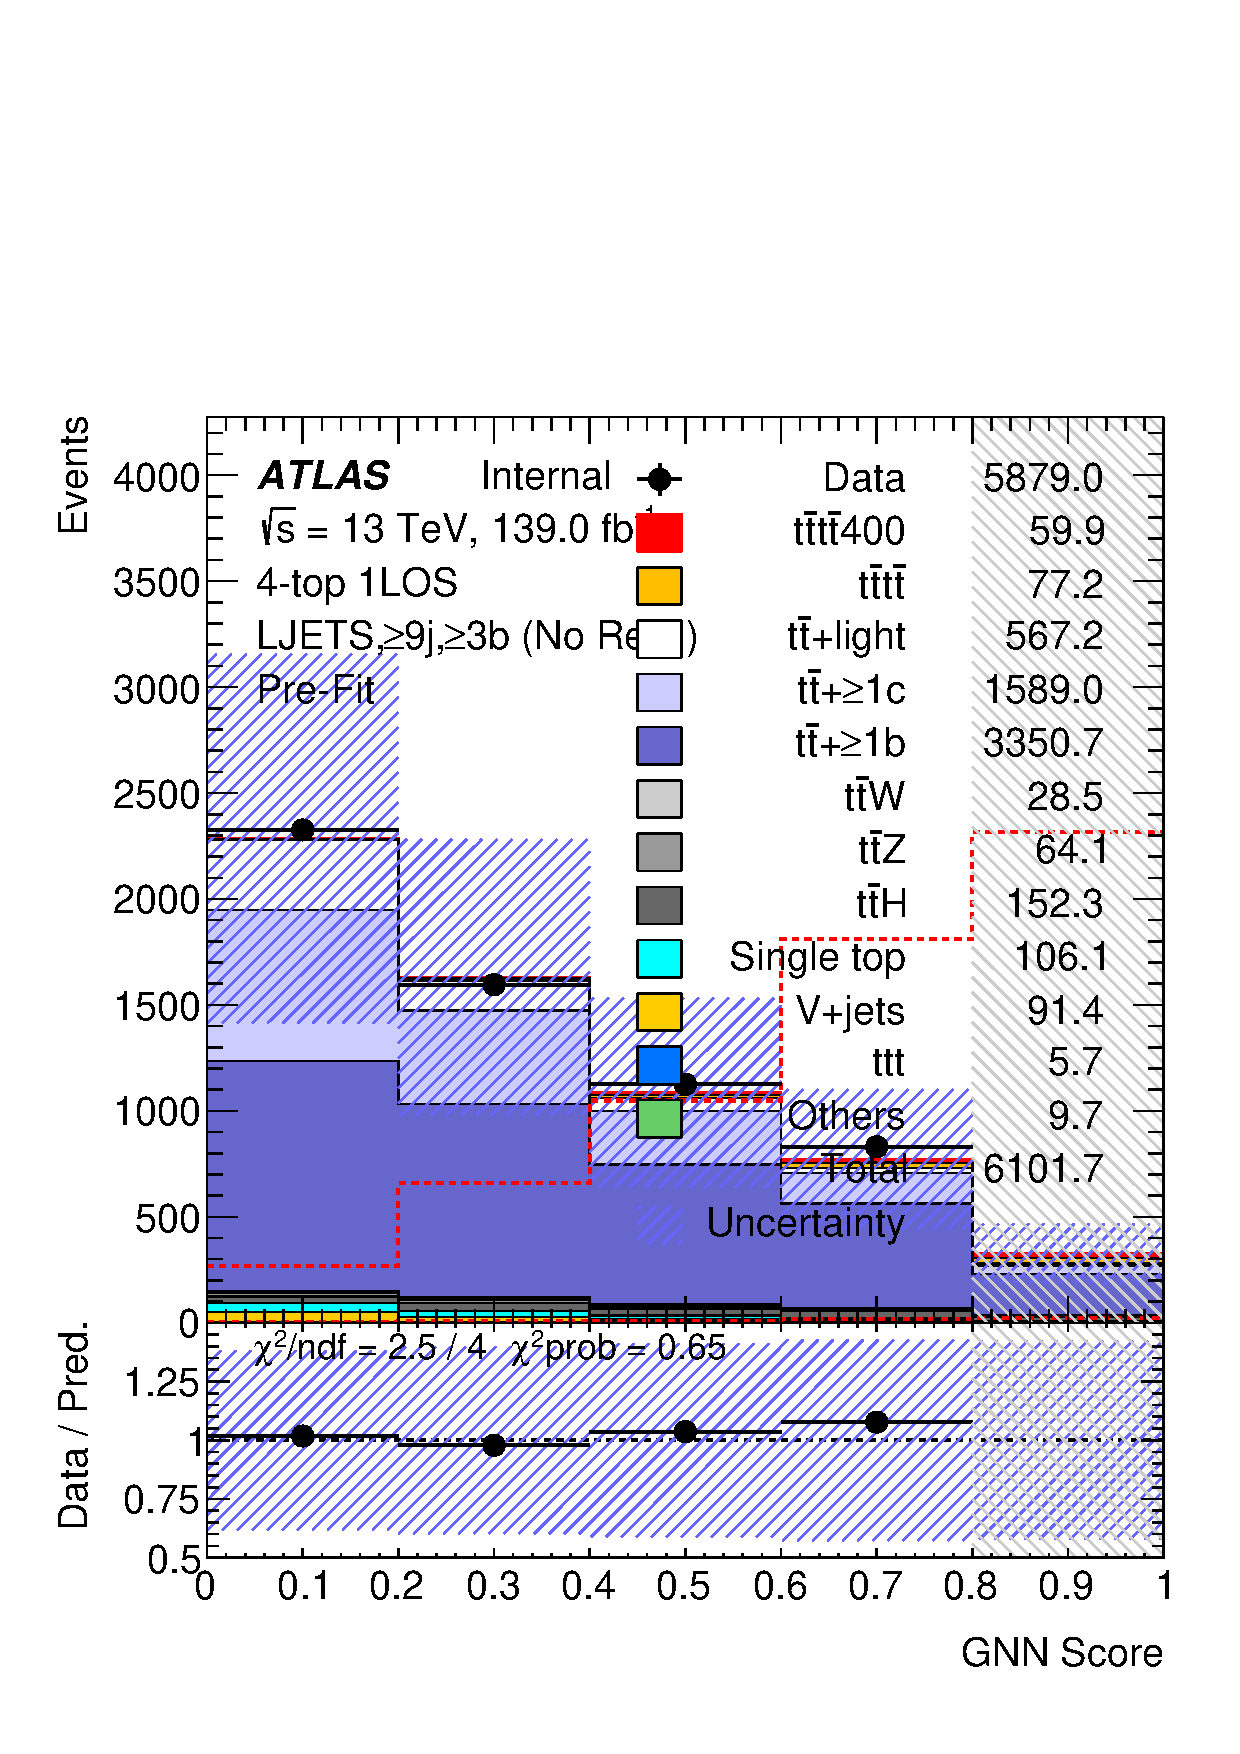
\includegraphics[width=0.3\textwidth]{figures/NNPlots/MVATrainRegion/NoRew/ljets_ge9jge3b_GNN.pdf}
    
\includegraphics[width=0.3\textwidth]{figures/NNPlots/MVATrainRegion/Rew/ljets_ge9jge3b_GNN.pdf}
    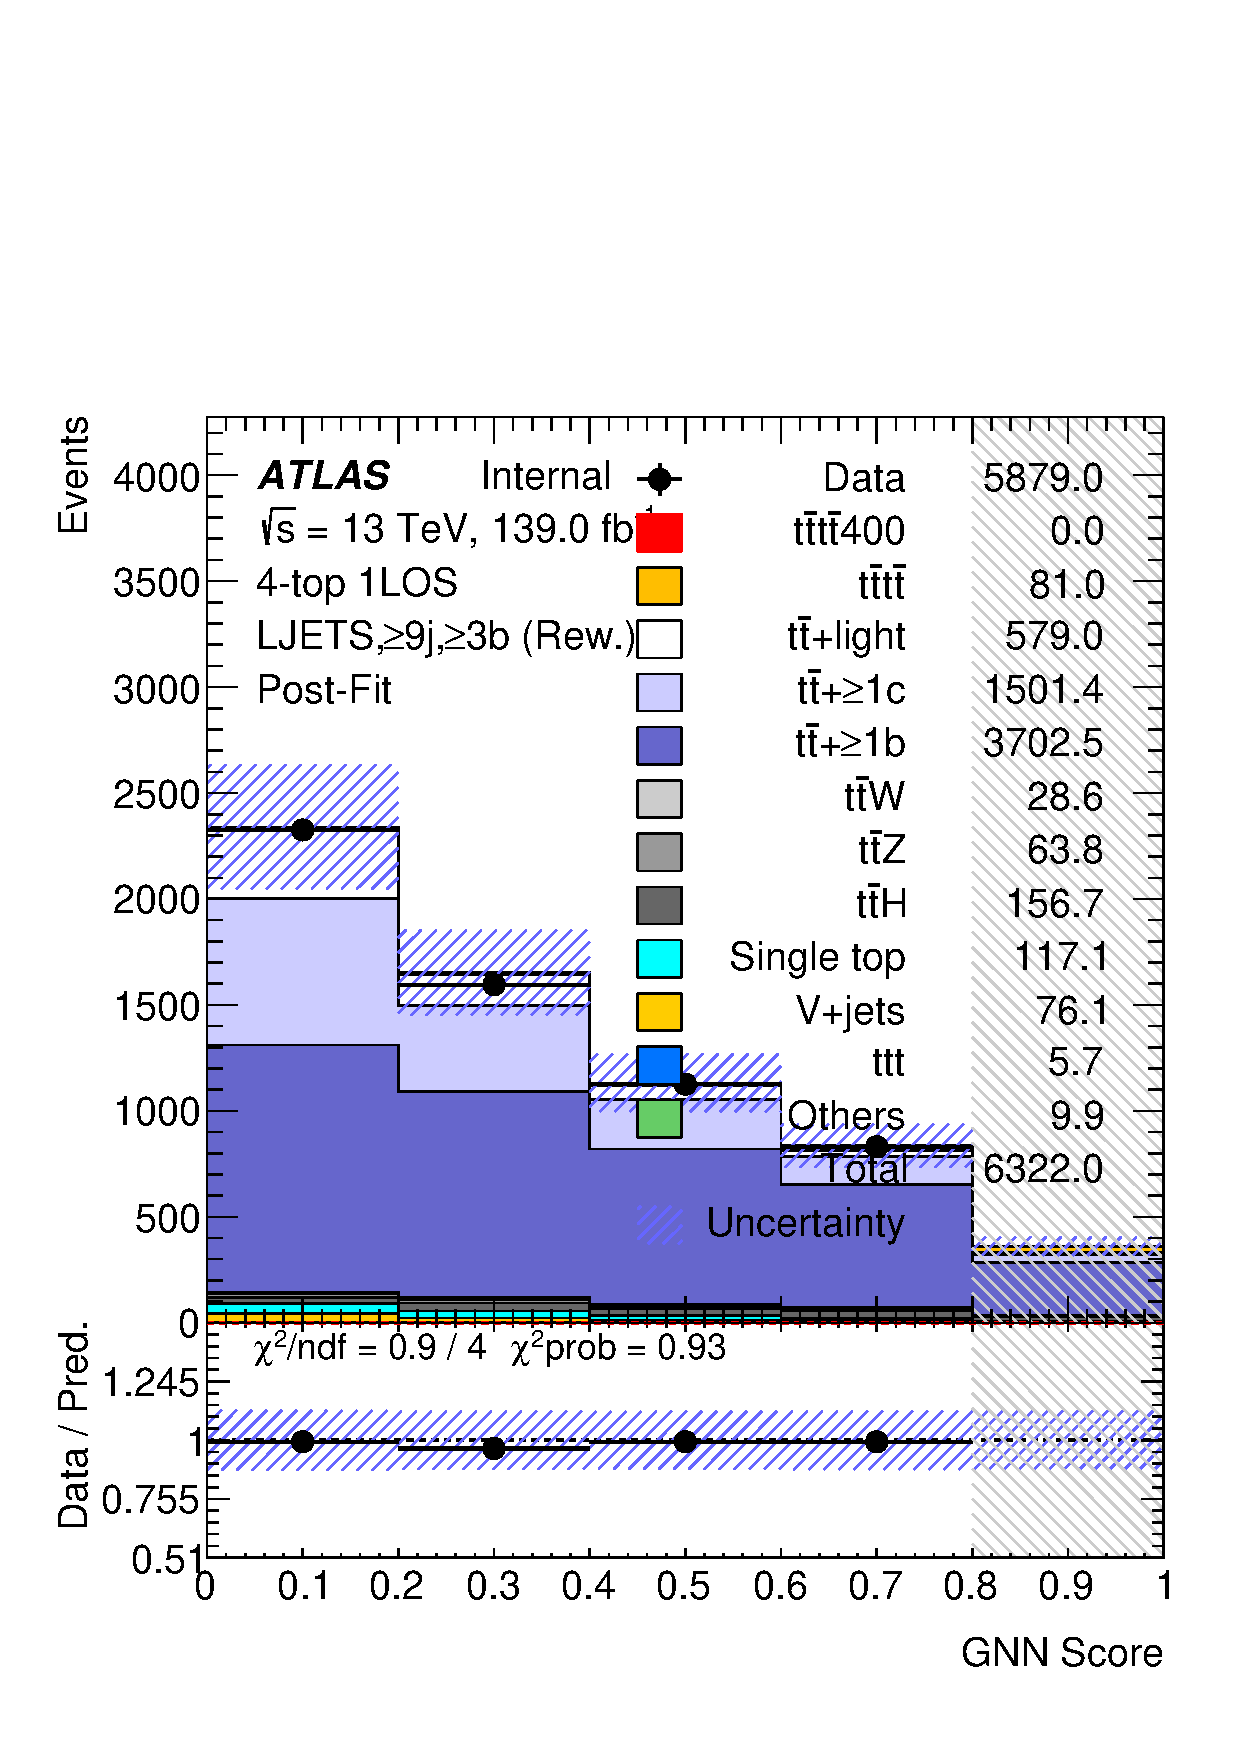
\includegraphics[width=0.3\textwidth]{figures/NNPlots/MVATrainRegion/Rew/ljets_ge9jge3b_GNN_postFit.pdf}
    \caption{GNN Score}
    \end{center}
    \end{subfigure}
    \caption{\label{fig:NNPlots_MVATrainReg_5} The comparison between variables pre-fit distribution before (left) and after (middle) the NN-reweighting  in 1L MVA training regions ($\geq 9j,\geq 3b$). The post-fit distribution after the NN-reweighting is shown on the left. Blinded regions are excluded.}
\end{figure}

%%% 2LOS %%%
\begin{figure}[htbp!]
    \begin{subfigure}[t]{1\textwidth}
    \begin{center}
    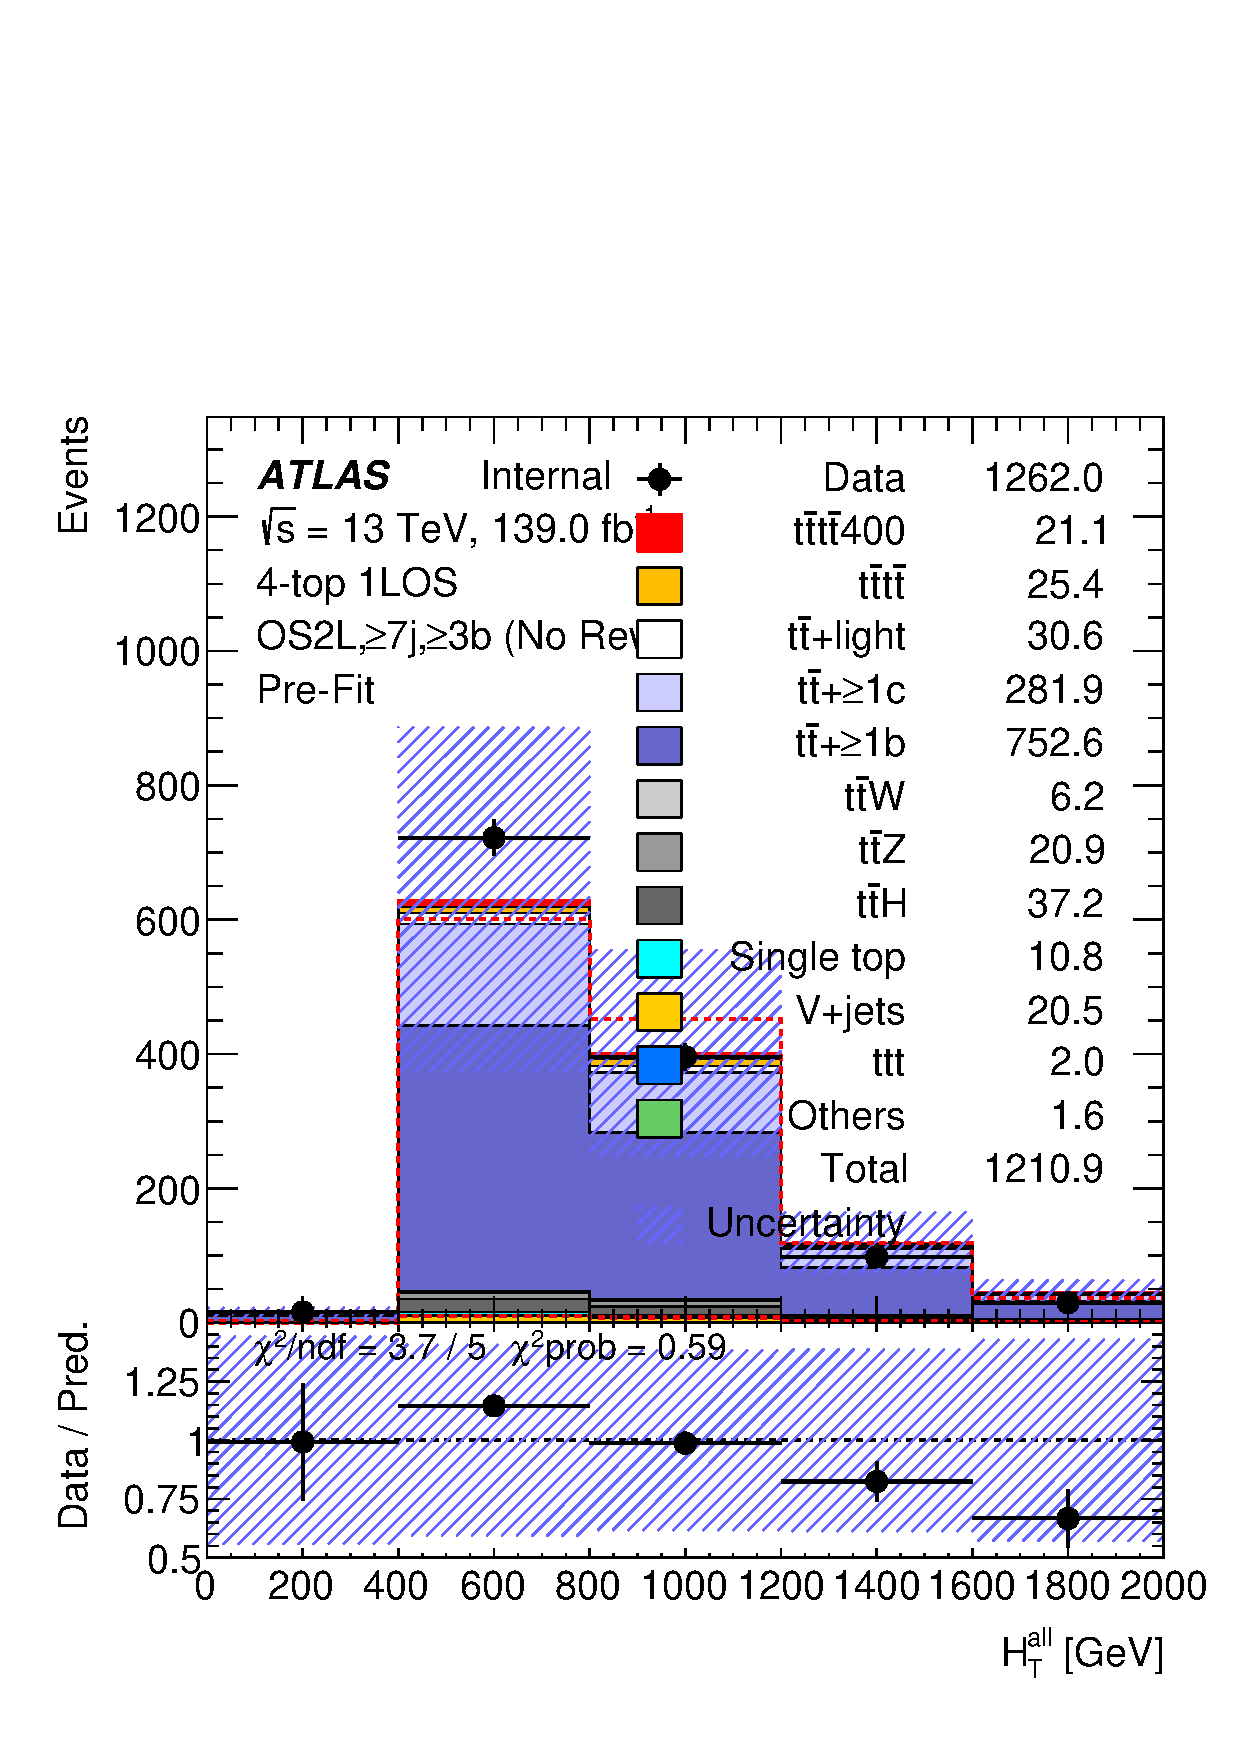
\includegraphics[width=0.3\textwidth]{figures/NNPlots/MVATrainRegion/NoRew/os2l_ge7jge3b_HT.pdf}
    
\includegraphics[width=0.3\textwidth]{figures/NNPlots/MVATrainRegion/Rew/os2l_ge7jge3b_HT.pdf}
    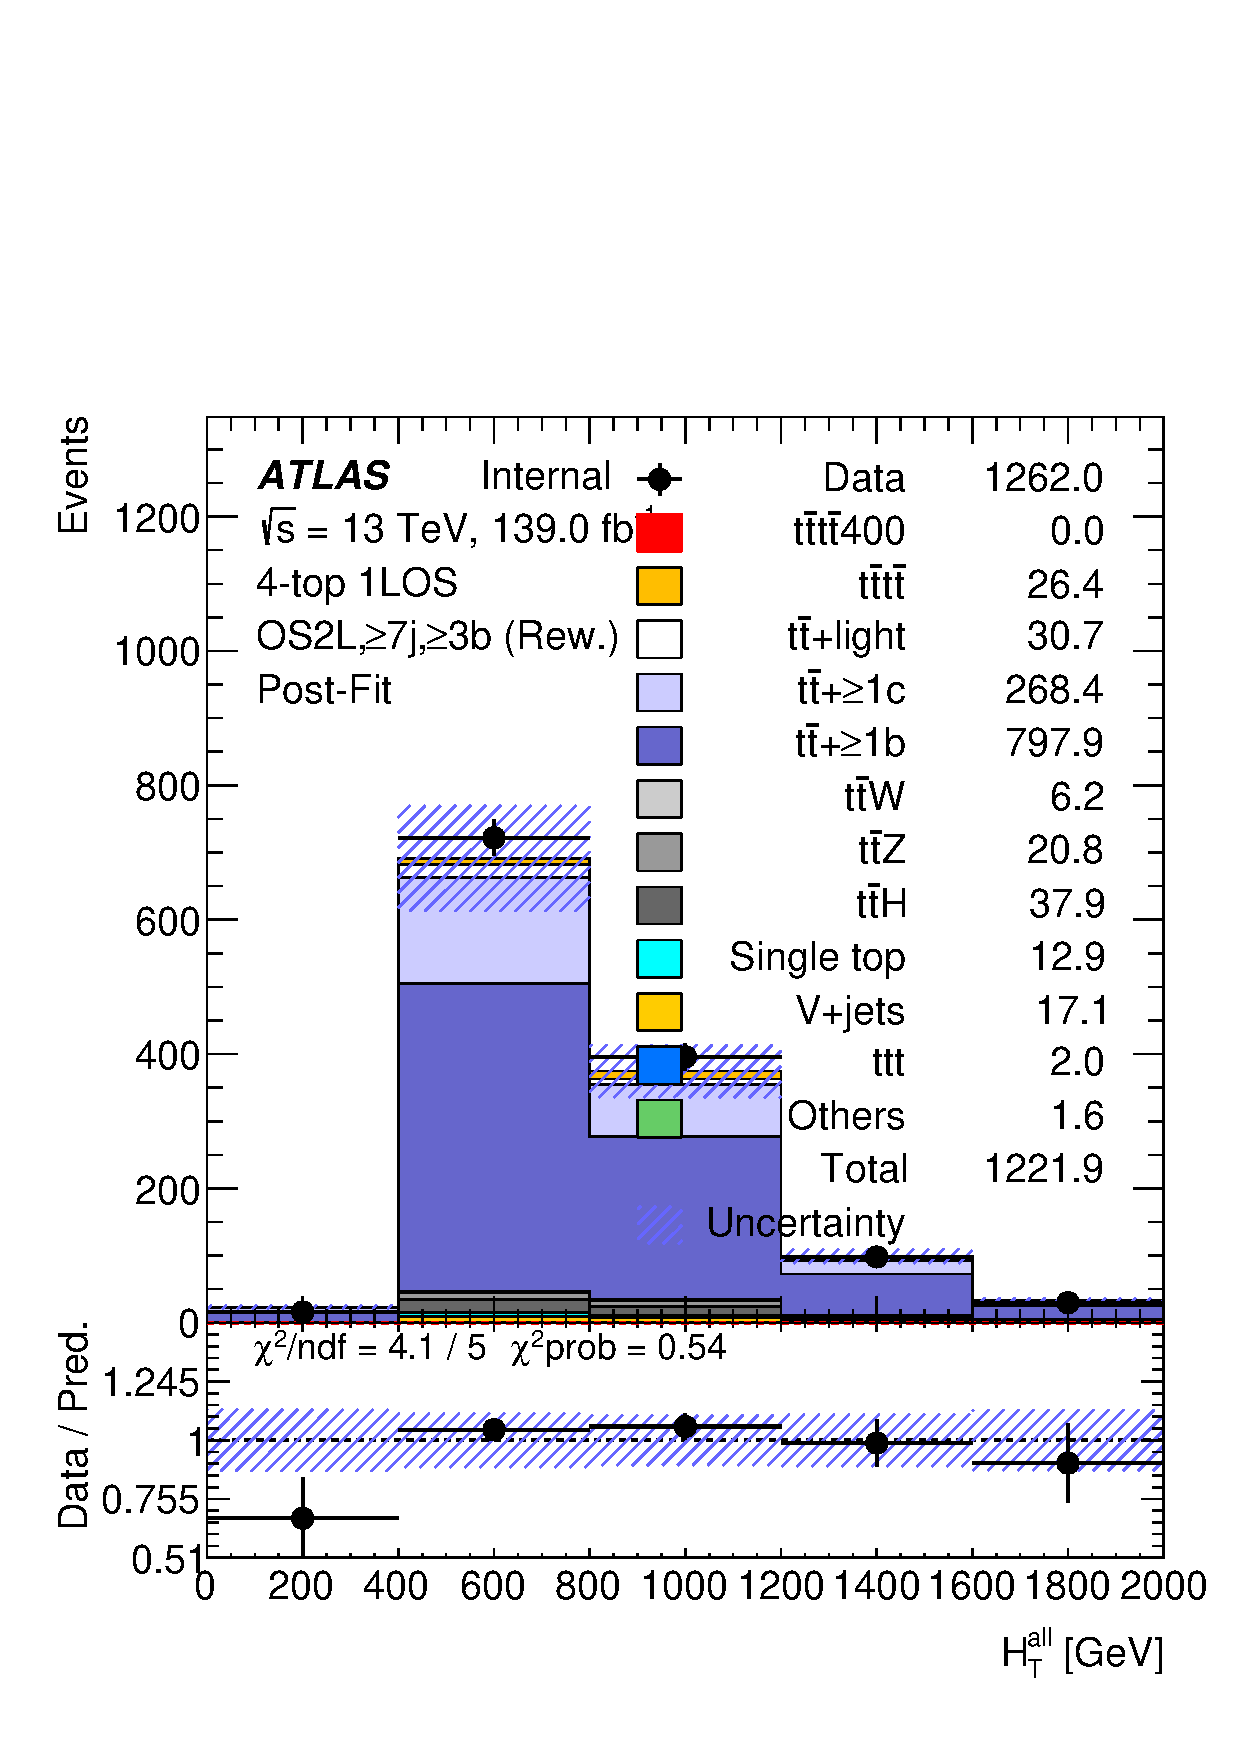
\includegraphics[width=0.3\textwidth]{figures/NNPlots/MVATrainRegion/Rew/os2l_ge7jge3b_HT_postFit.pdf}
    \caption{$H_{T}$}
    \end{center}
    \end{subfigure}

    \begin{subfigure}[t]{1\textwidth}
    \begin{center}
    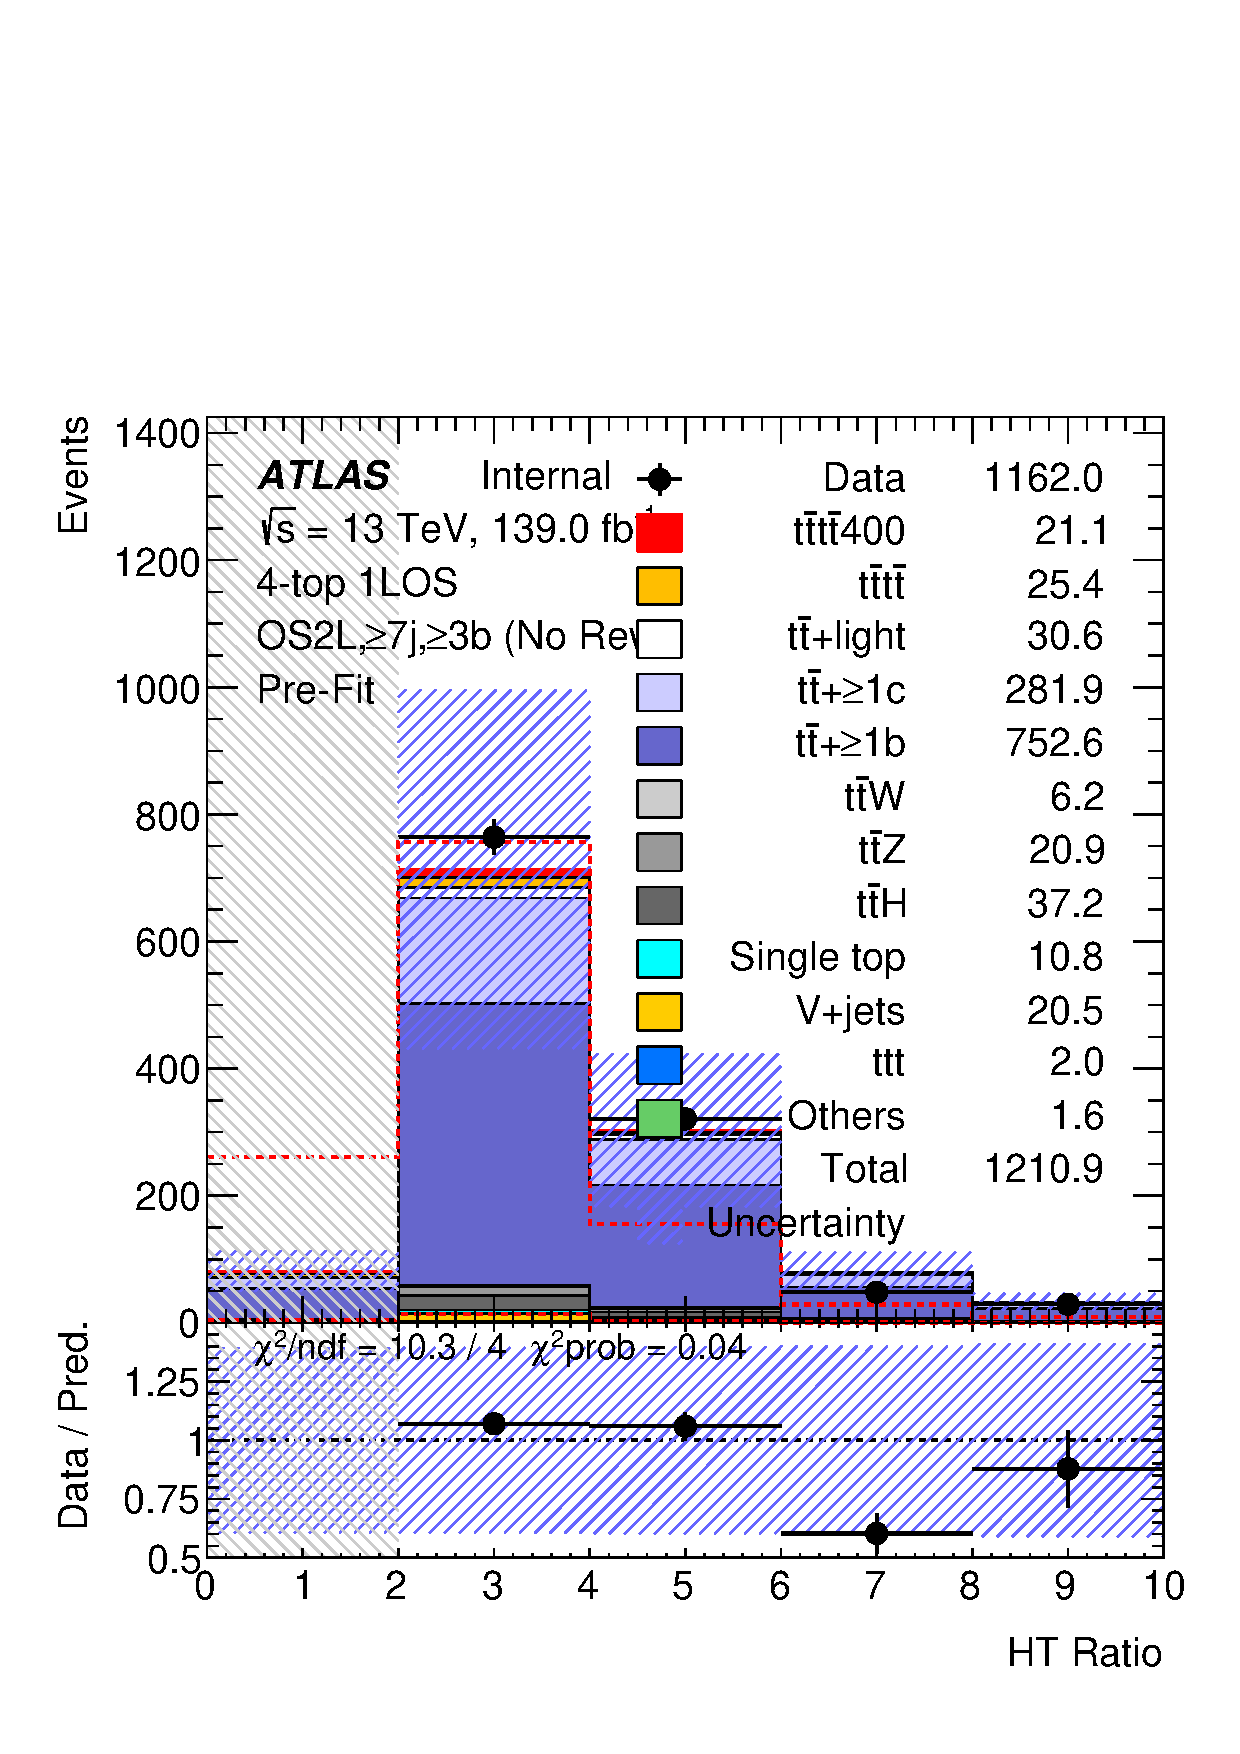
\includegraphics[width=0.3\textwidth]{figures/NNPlots/MVATrainRegion/NoRew/os2l_ge7jge3b_HTRatio.pdf}
    
\includegraphics[width=0.3\textwidth]{figures/NNPlots/MVATrainRegion/Rew/os2l_ge7jge3b_HTRatio.pdf}
    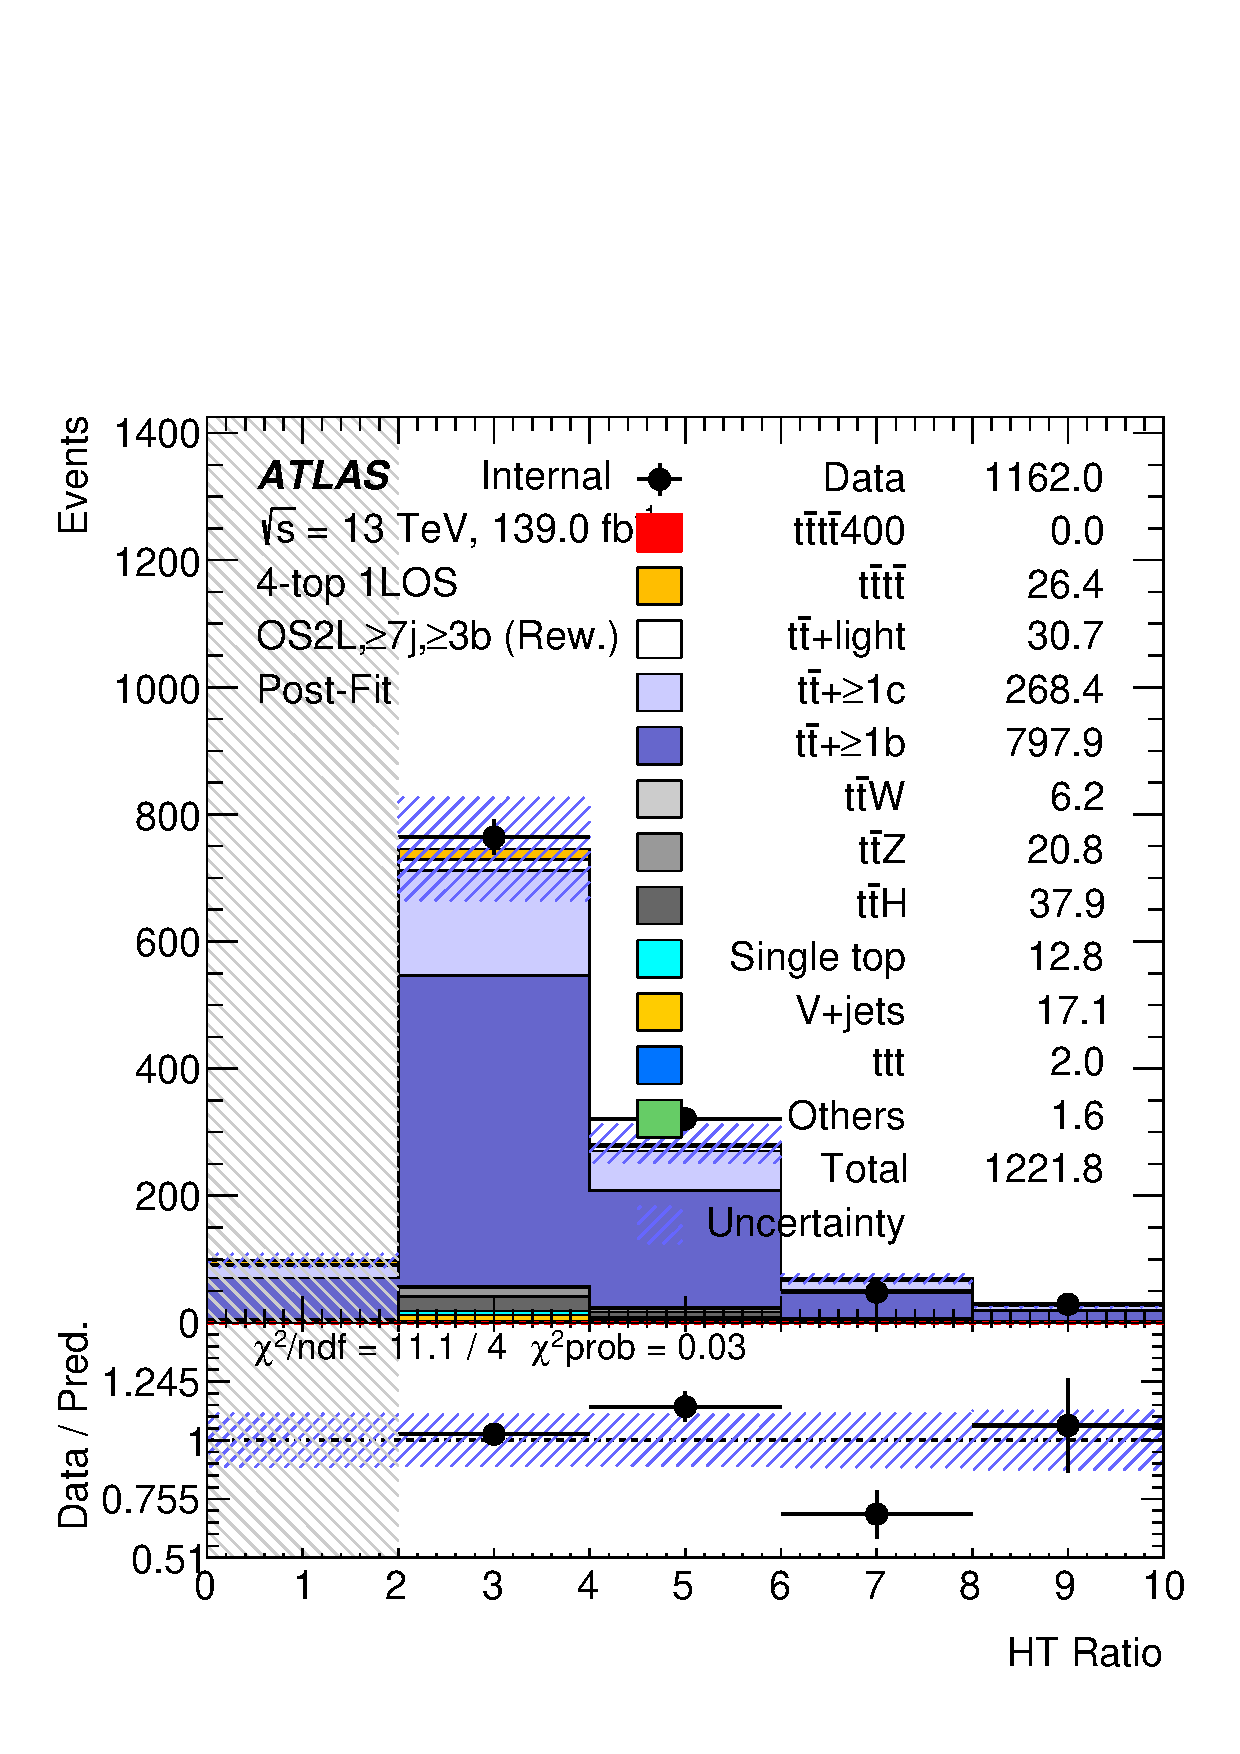
\includegraphics[width=0.3\textwidth]{figures/NNPlots/MVATrainRegion/Rew/os2l_ge7jge3b_HTRatio_postFit.pdf}
    \caption{HTRatio}
    \end{center}
    \end{subfigure}

    \begin{subfigure}[t]{1\textwidth}
    \begin{center}
    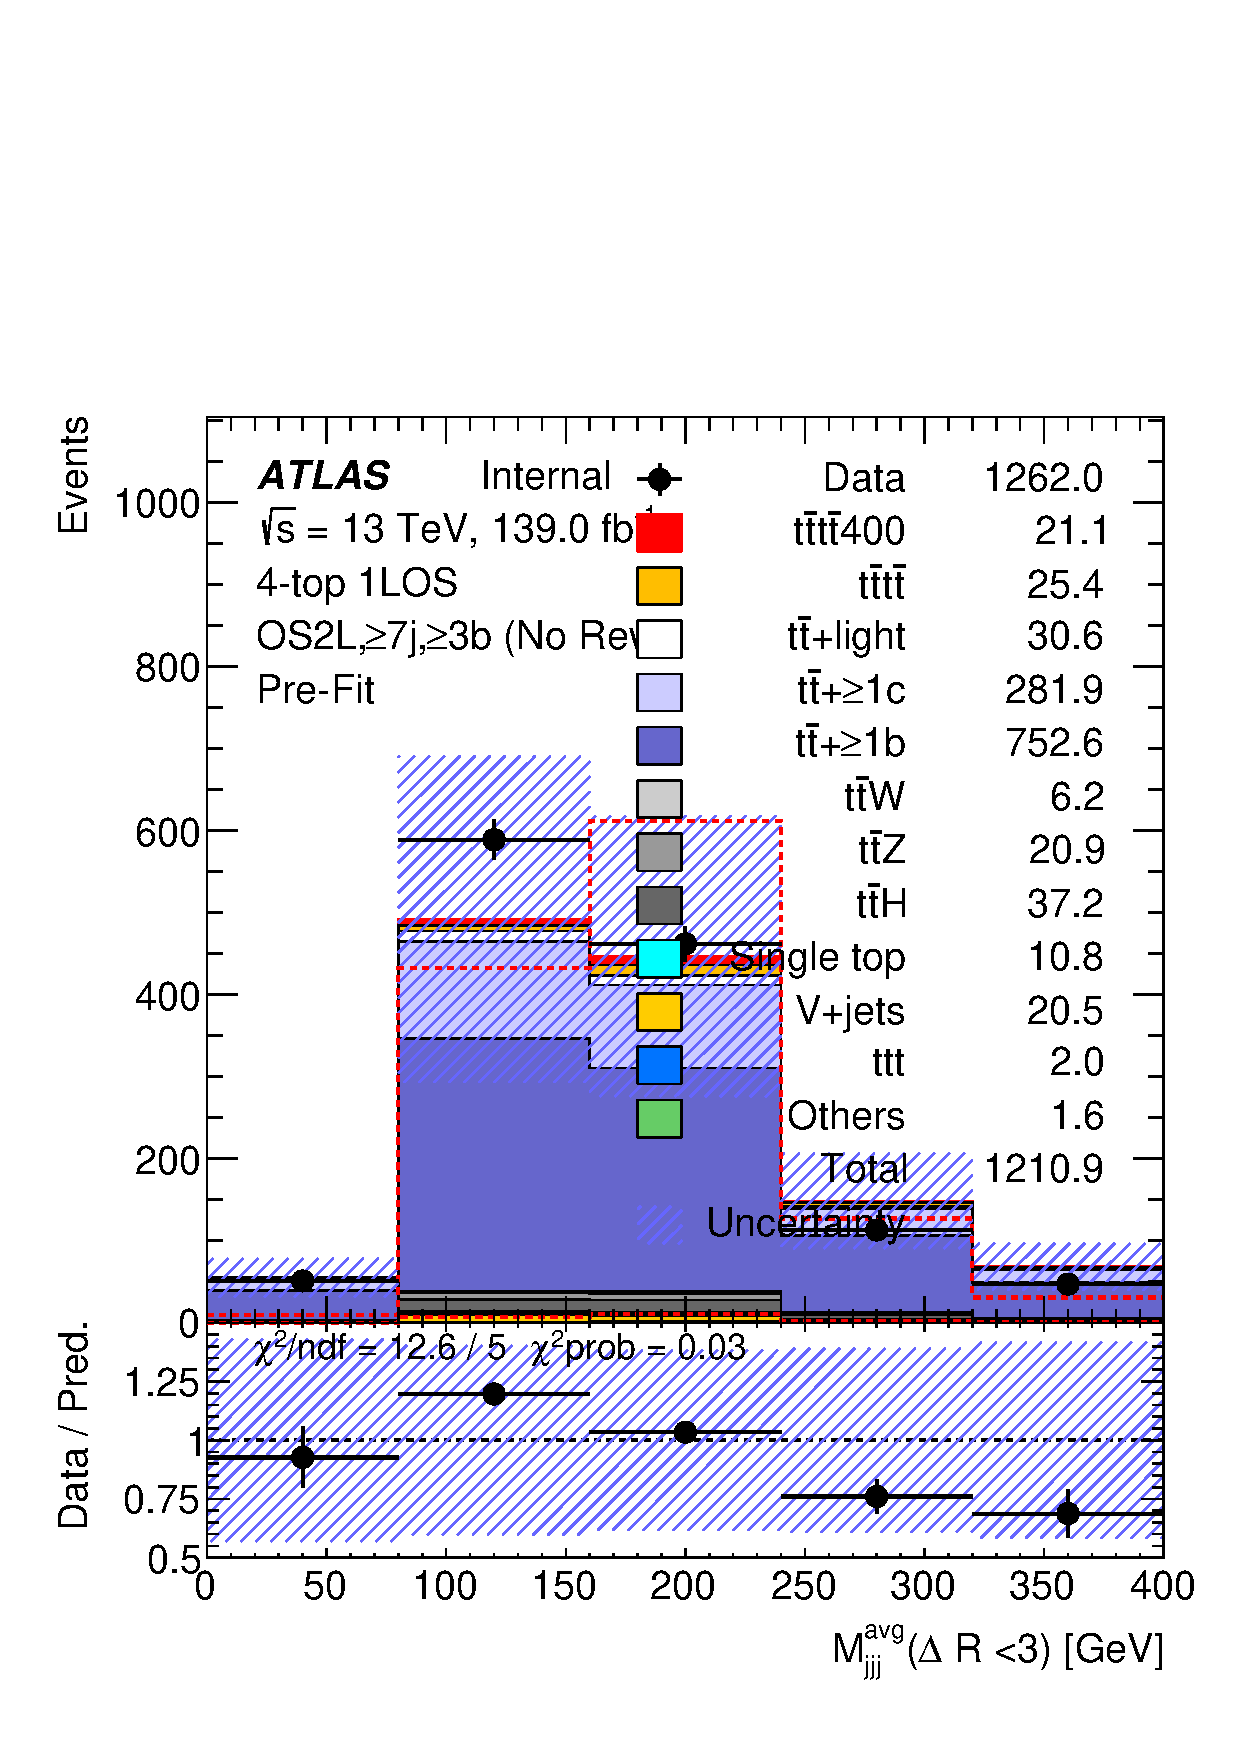
\includegraphics[width=0.3\textwidth]{figures/NNPlots/MVATrainRegion/NoRew/os2l_ge7jge3b_Mjjj_AvgdRs3.pdf}
    
\includegraphics[width=0.3\textwidth]{figures/NNPlots/MVATrainRegion/Rew/os2l_ge7jge3b_Mjjj_AvgdRs3.pdf}
    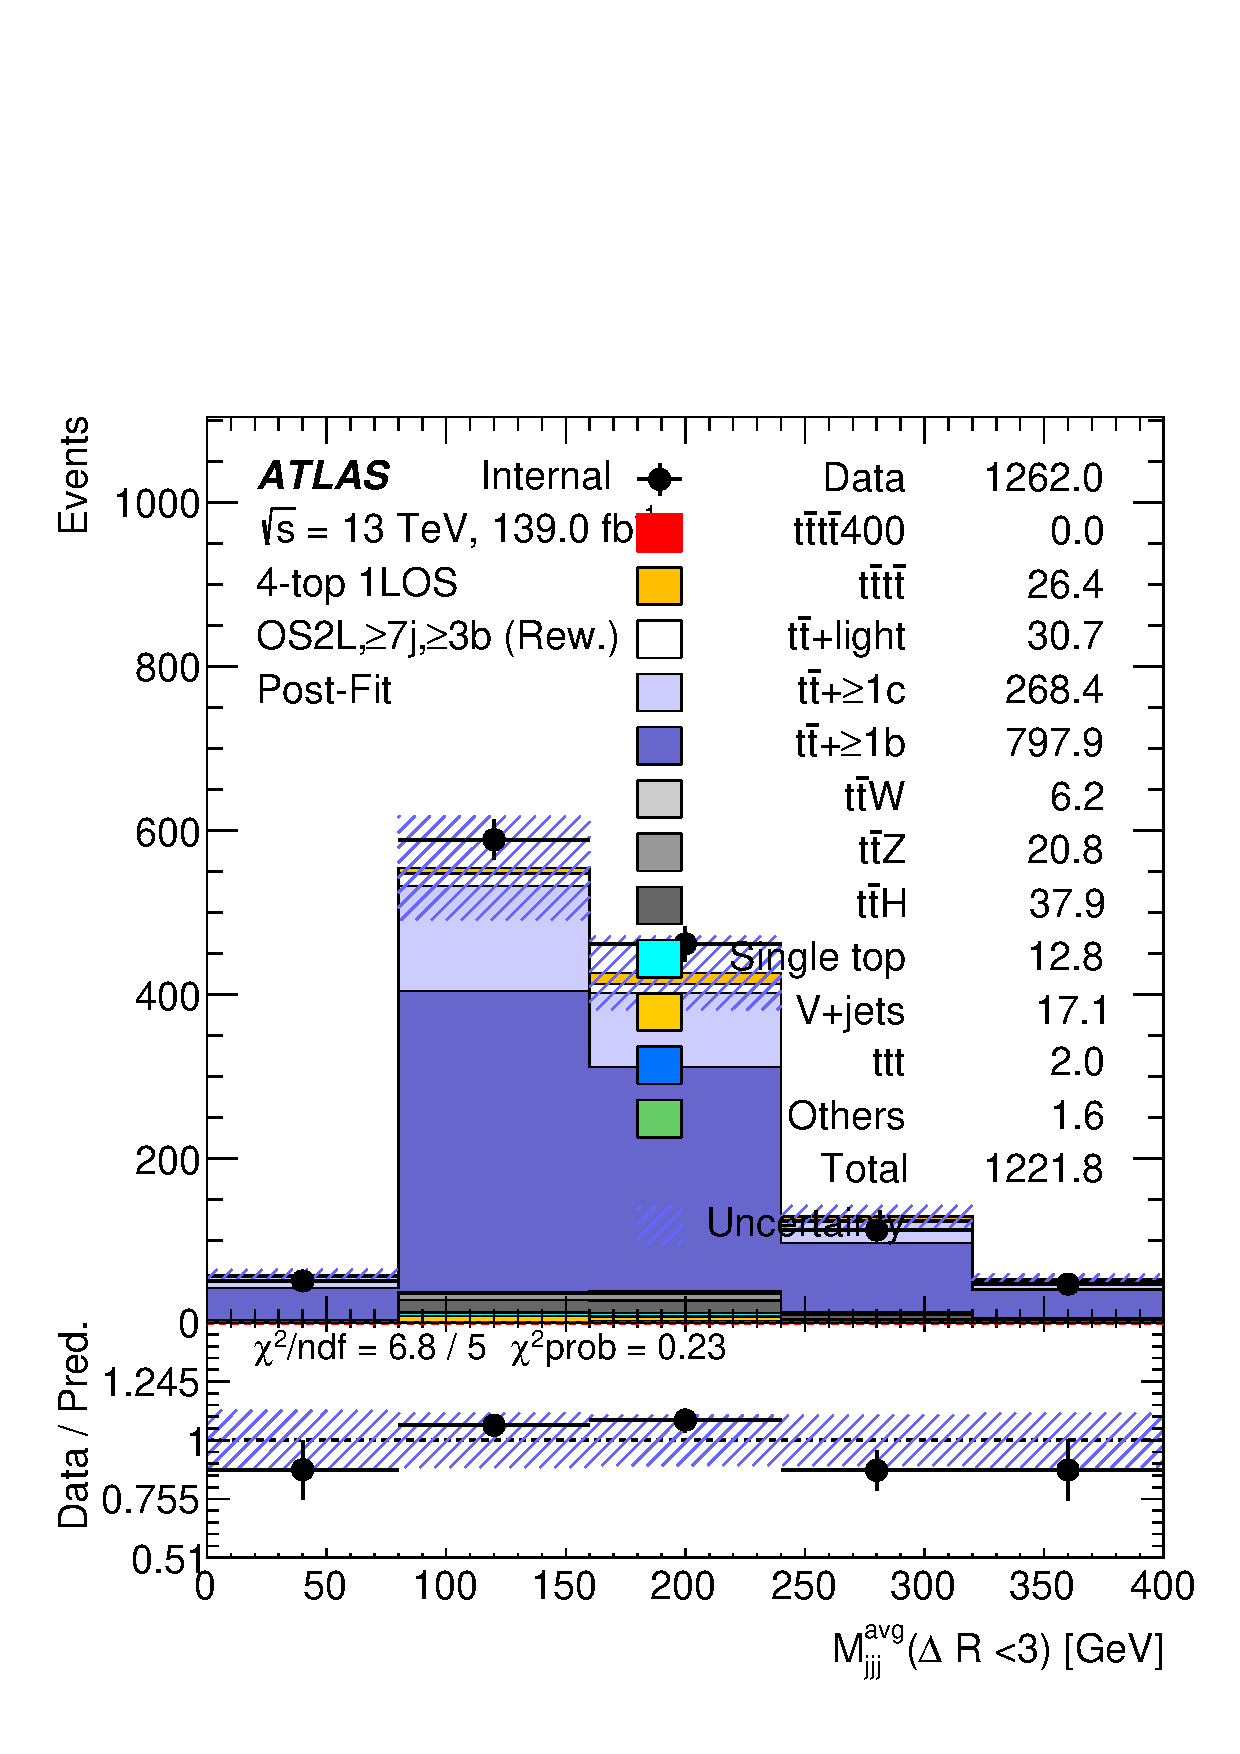
\includegraphics[width=0.3\textwidth]{figures/NNPlots/MVATrainRegion/Rew/os2l_ge7jge3b_Mjjj_AvgdRs3_postFit.pdf}
    \caption{$M^{avg}_{jjj}(\Delta R <3)$}
    \end{center}
    \end{subfigure}
    \caption{\label{fig:NNPlots_MVATrainReg_6} The comparison between variables pre-fit distribution before (left) and after (middle) the NN-reweighting  in 1L MVA training regions ($\geq 7j,\geq 3b$). The post-fit distribution after the NN-reweighting is shown on the left. Blinded regions are excluded.}  
\end{figure}

\begin{figure}[htbp!]
    \begin{subfigure}[t]{1\textwidth}
    \begin{center}
    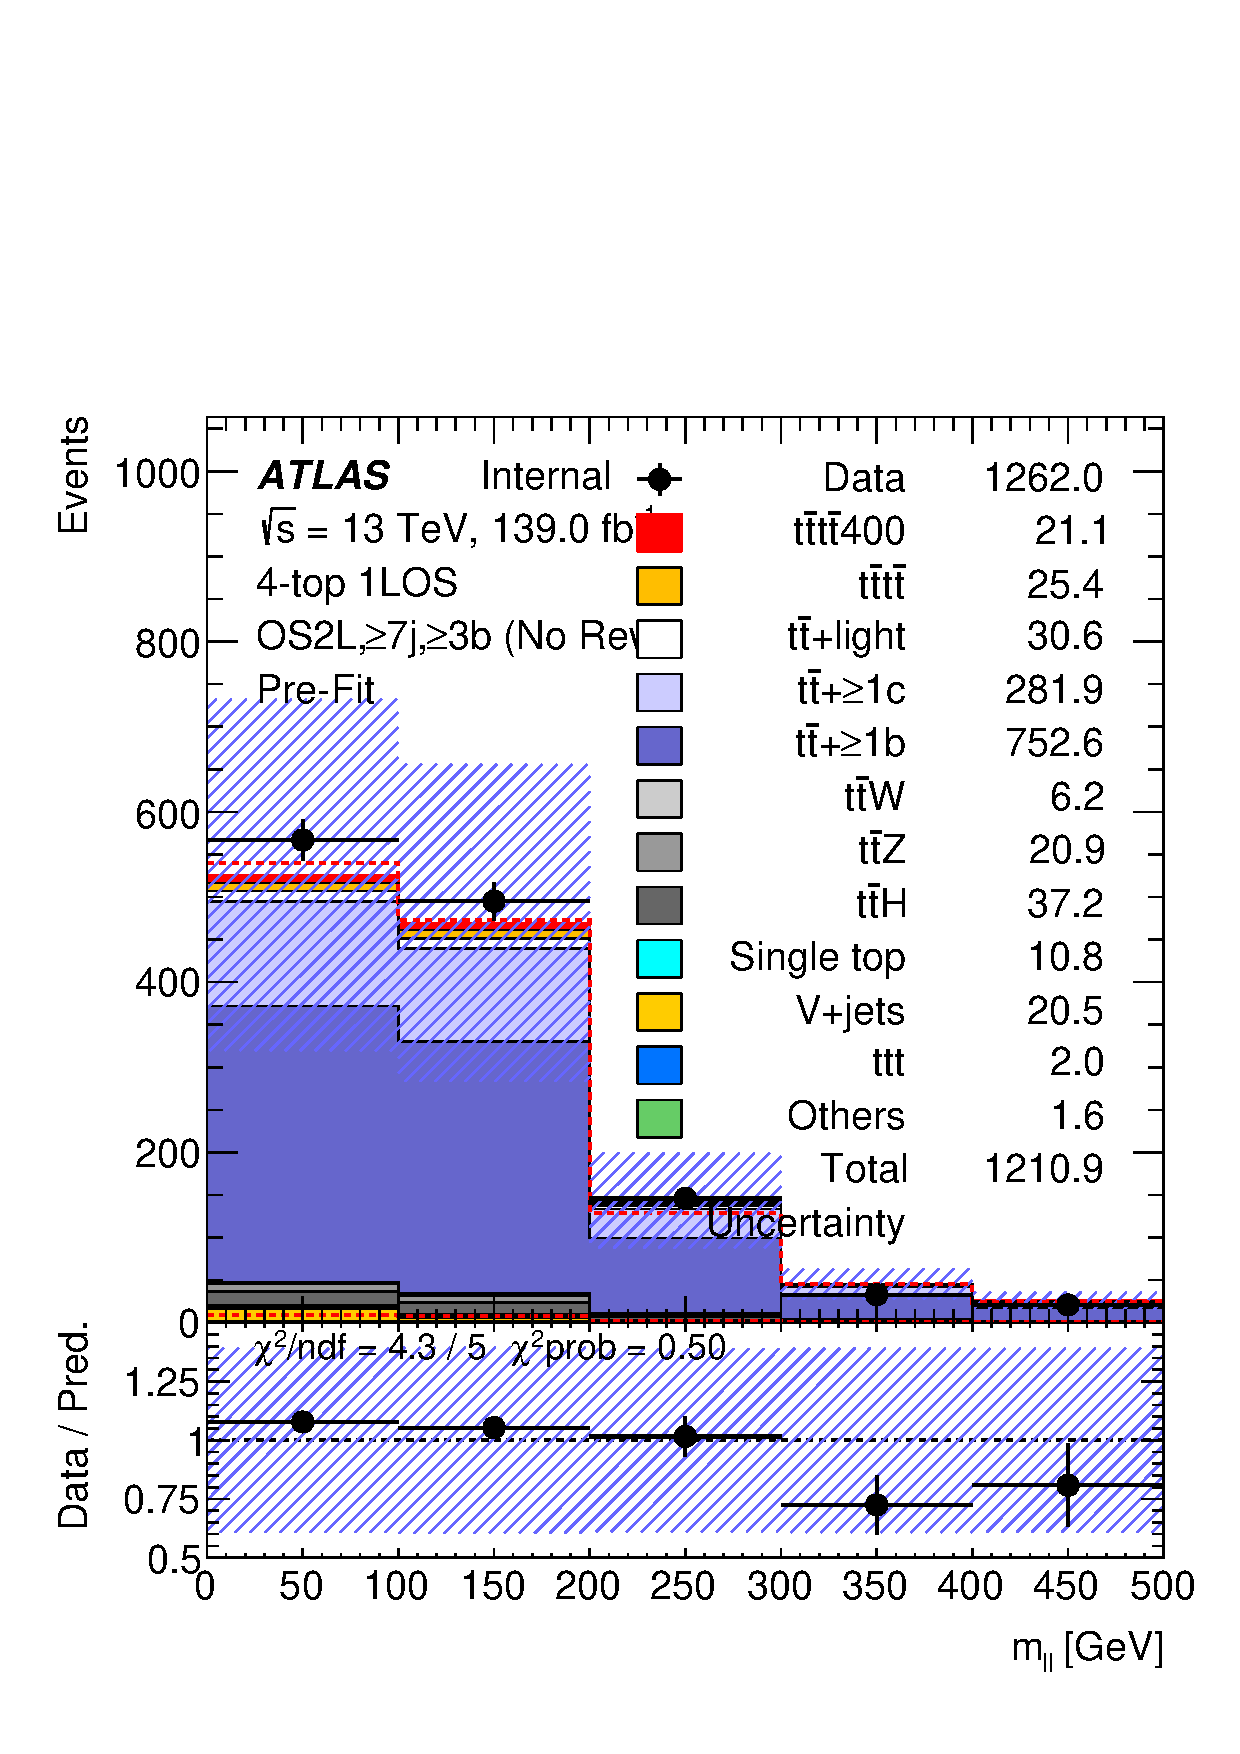
\includegraphics[width=0.3\textwidth]{figures/NNPlots/MVATrainRegion/NoRew/os2l_ge7jge3b_mll.pdf}
    
\includegraphics[width=0.3\textwidth]{figures/NNPlots/MVATrainRegion/Rew/os2l_ge7jge3b_mll.pdf}
    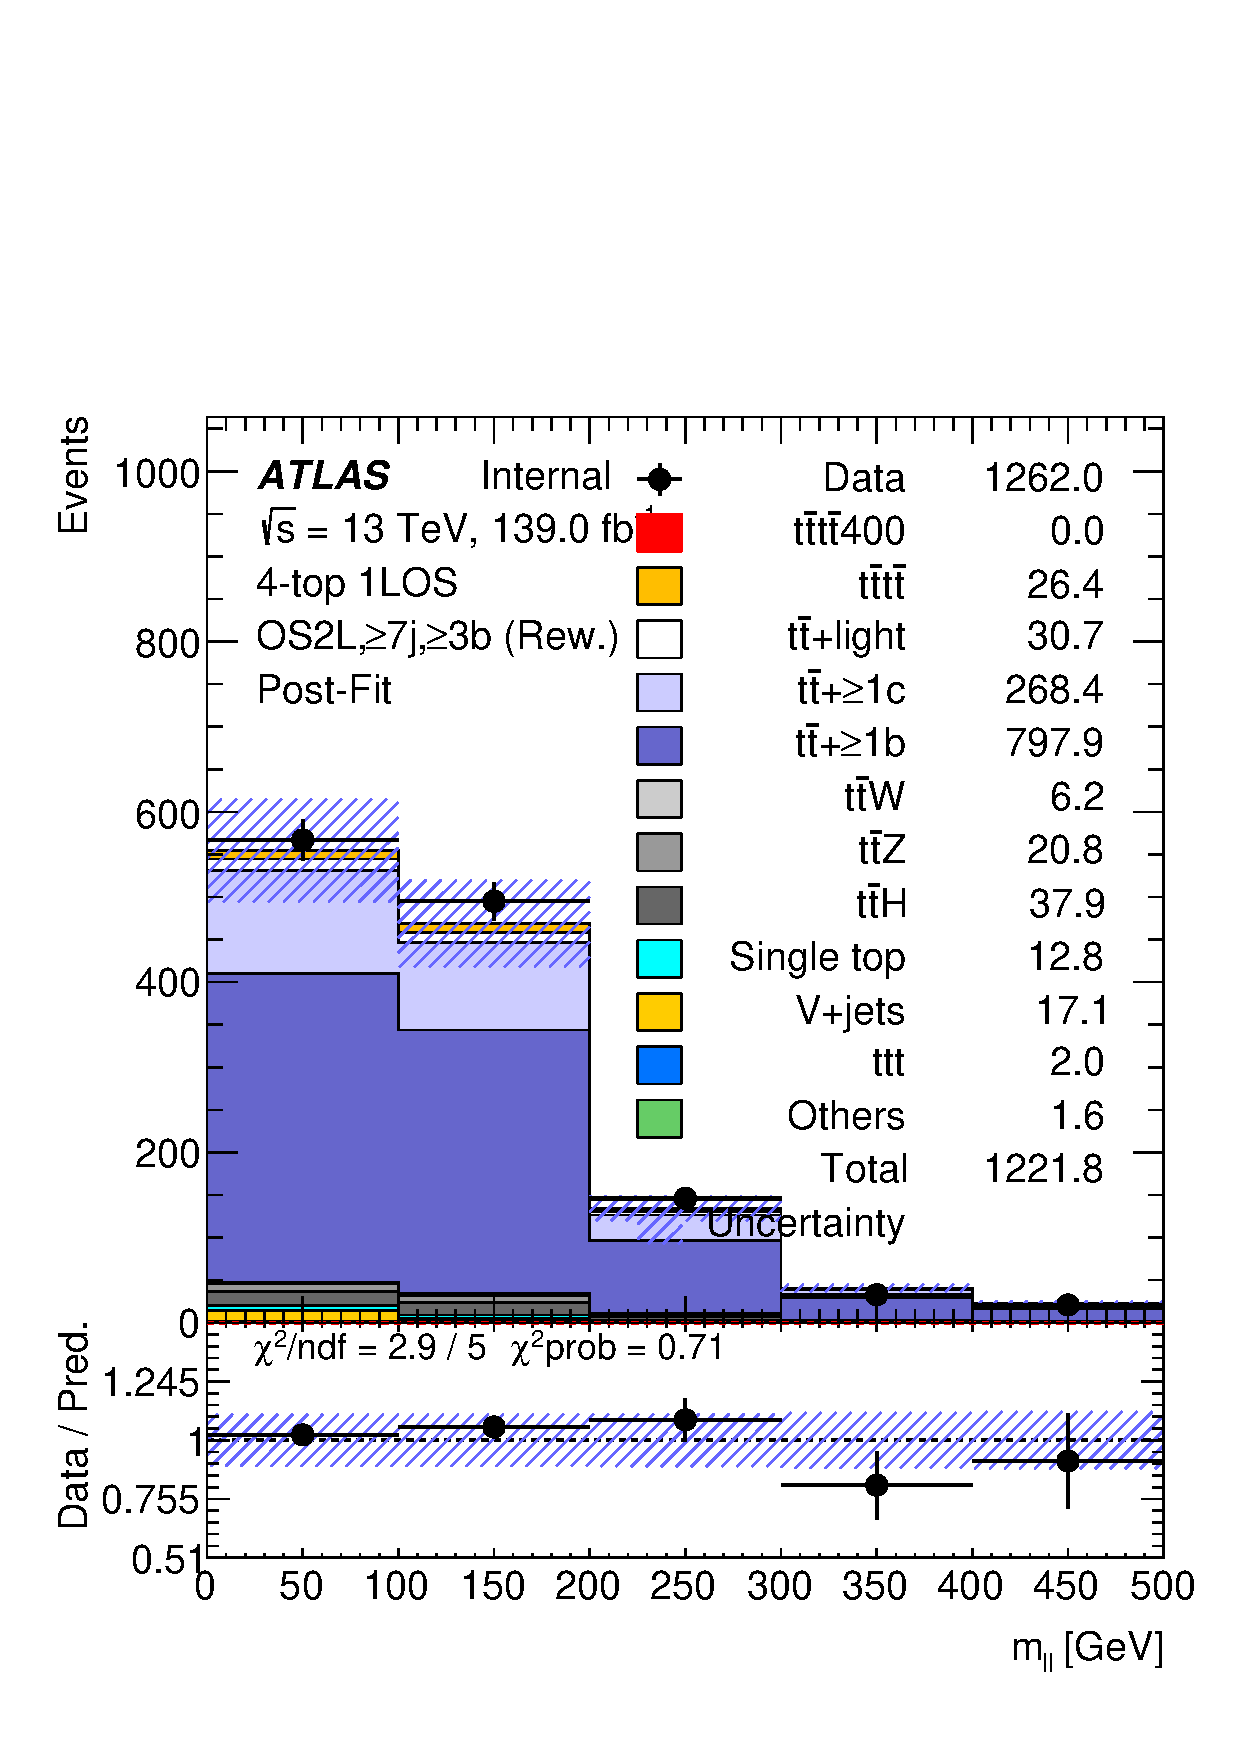
\includegraphics[width=0.3\textwidth]{figures/NNPlots/MVATrainRegion/Rew/os2l_ge7jge3b_mll_postFit.pdf}
    \caption{mll}
    \end{center}
    \end{subfigure}

    \begin{subfigure}[t]{1\textwidth}
    \begin{center}
    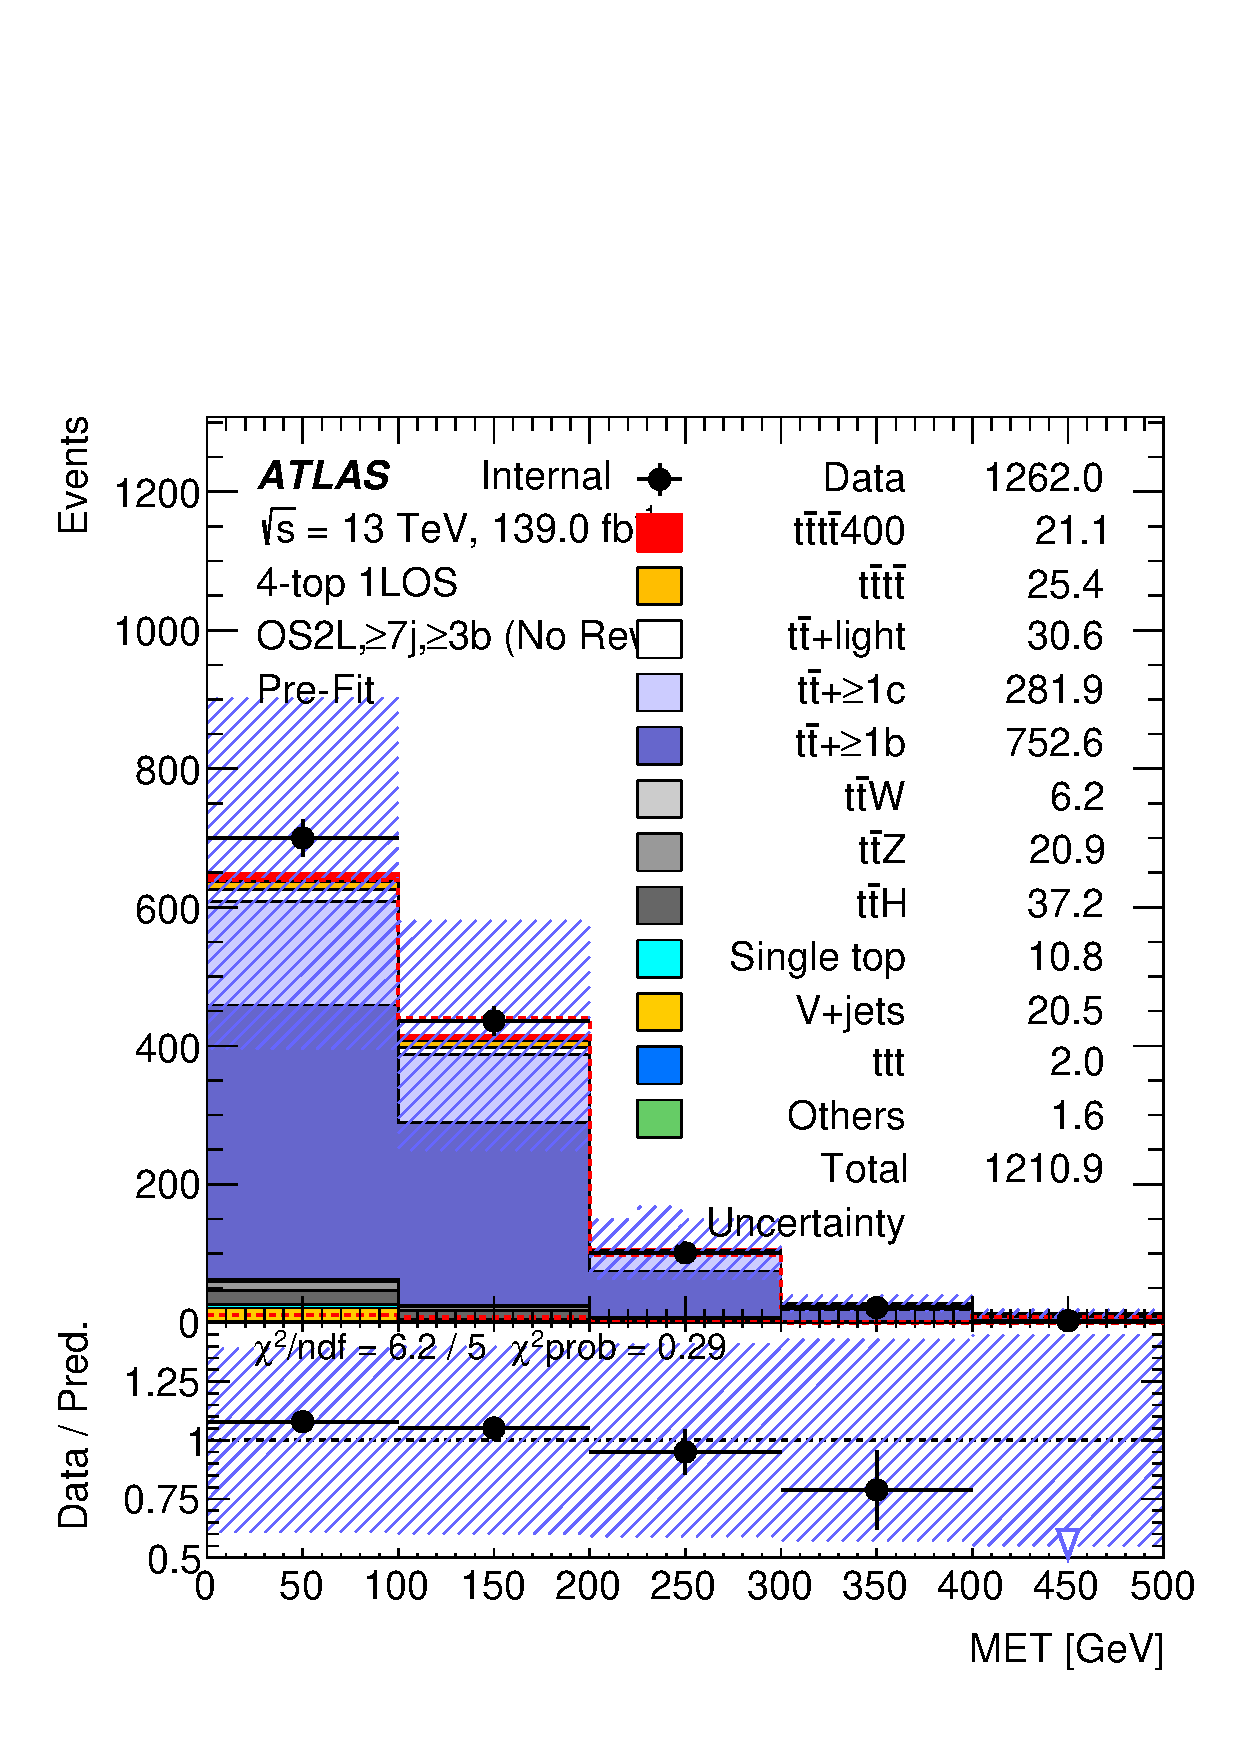
\includegraphics[width=0.3\textwidth]{figures/NNPlots/MVATrainRegion/NoRew/os2l_ge7jge3b_met.pdf}
    
\includegraphics[width=0.3\textwidth]{figures/NNPlots/MVATrainRegion/Rew/os2l_ge7jge3b_met.pdf}
    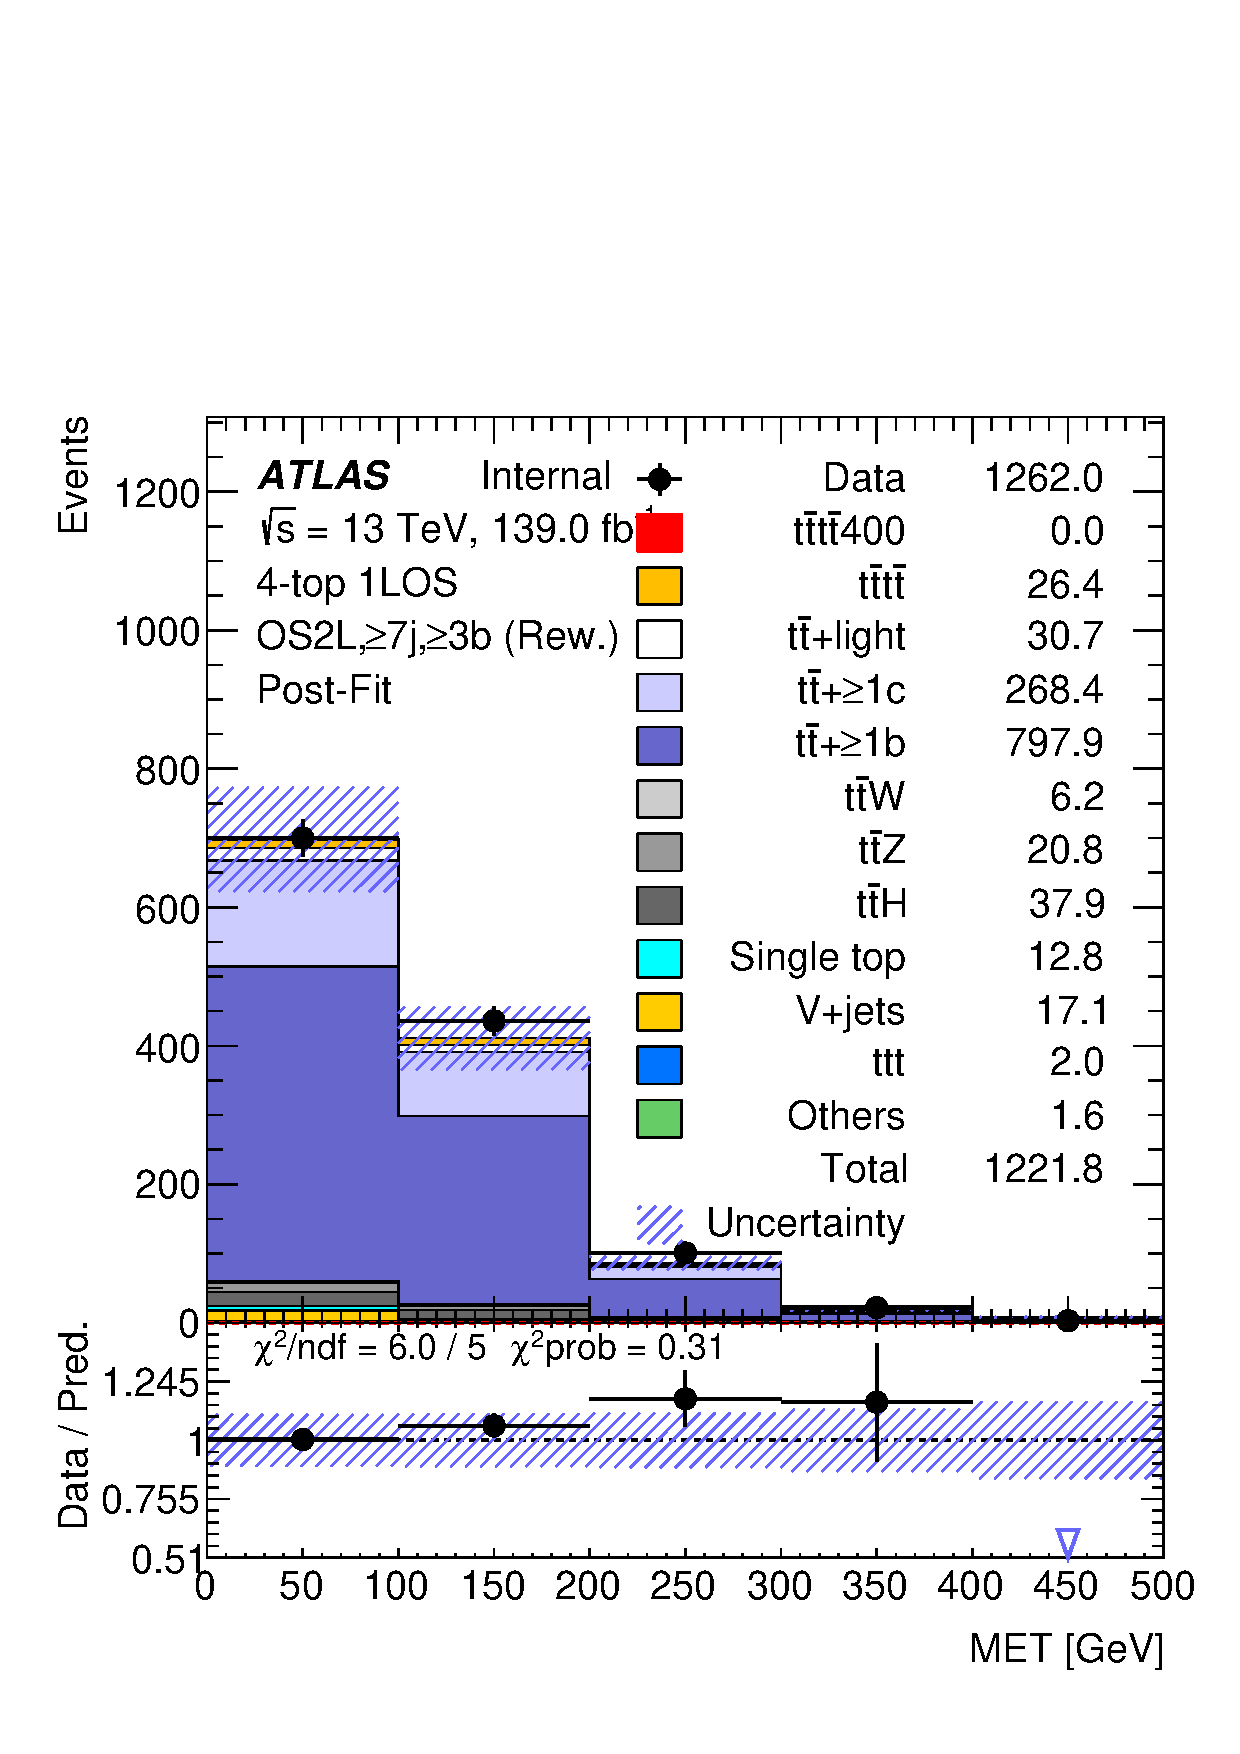
\includegraphics[width=0.3\textwidth]{figures/NNPlots/MVATrainRegion/Rew/os2l_ge7jge3b_met_postFit.pdf}
    \caption{MET}
    \end{center}
    \end{subfigure}

    \begin{subfigure}[t]{1\textwidth}
    \begin{center}
    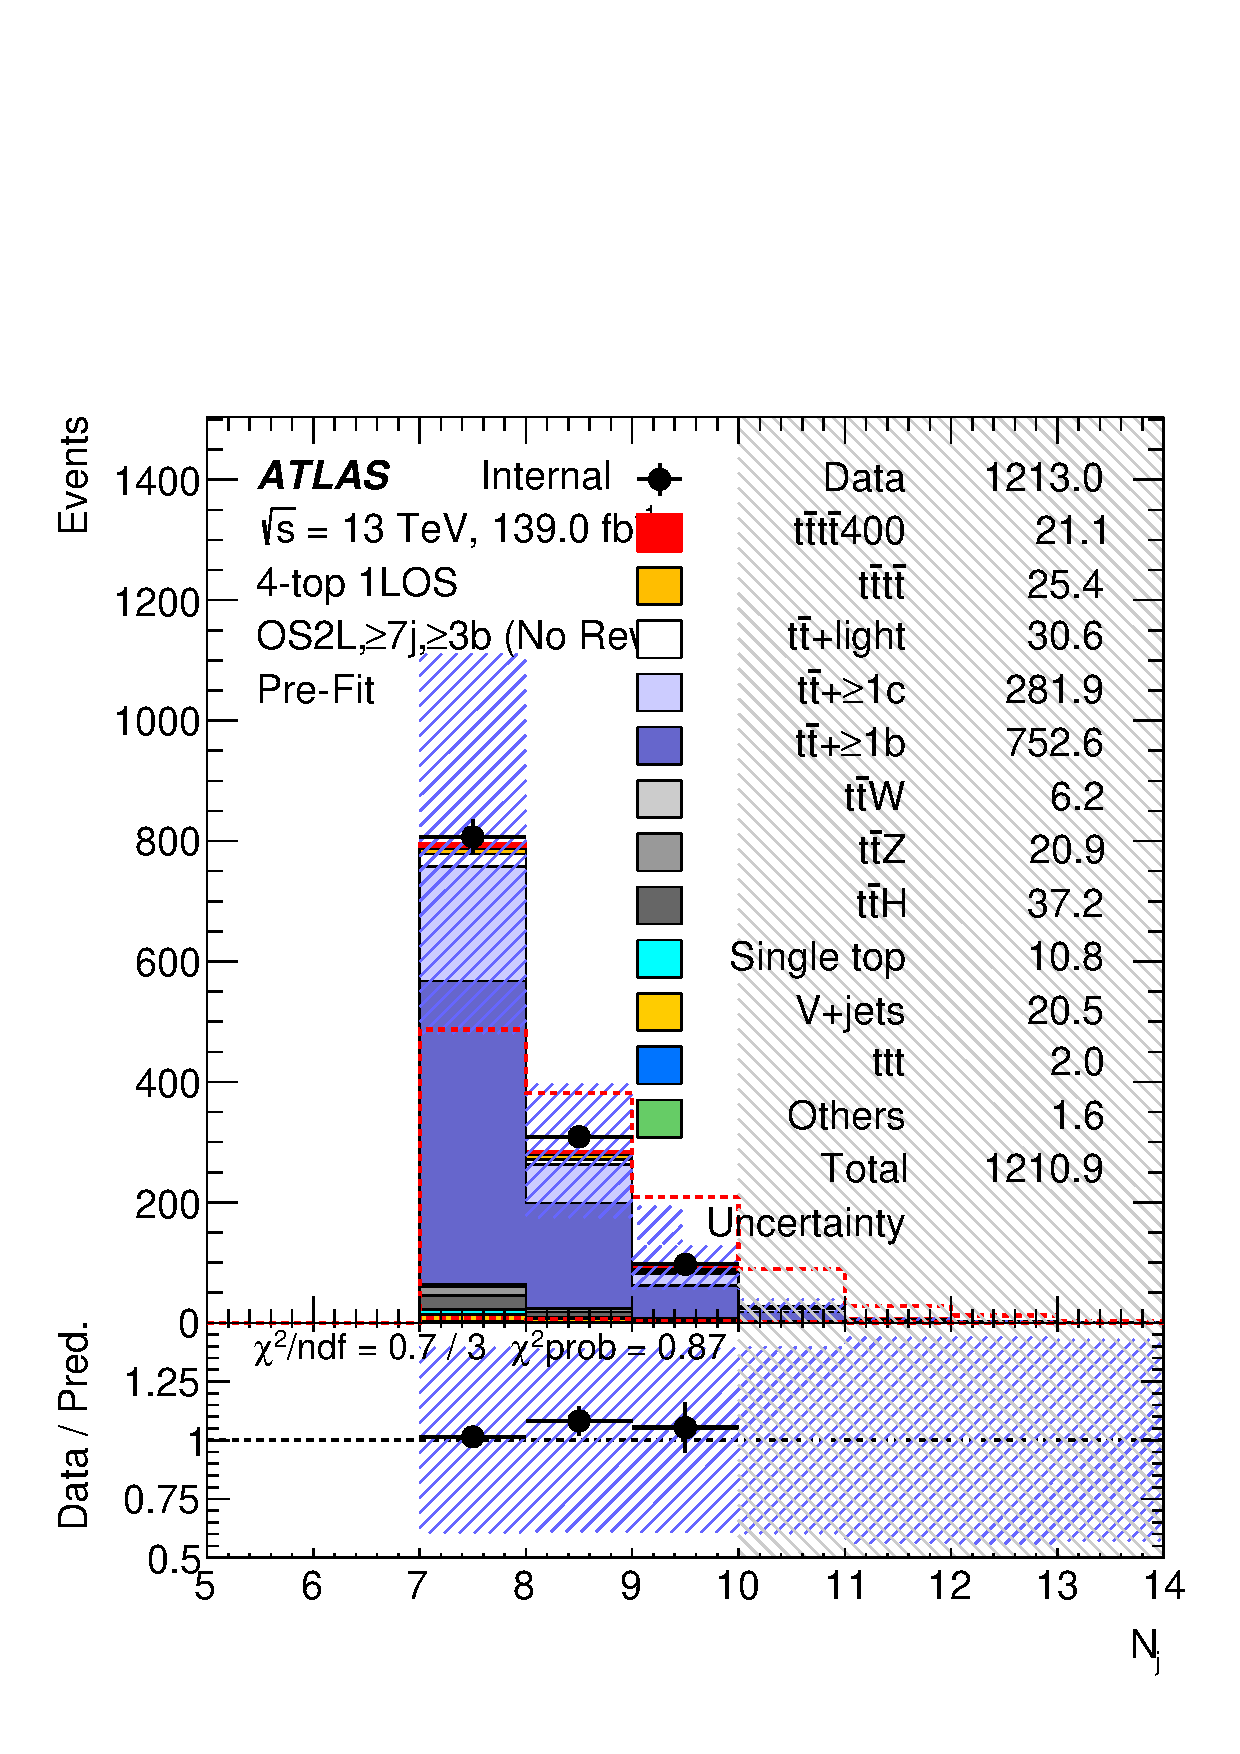
\includegraphics[width=0.3\textwidth]{figures/NNPlots/MVATrainRegion/NoRew/os2l_ge7jge3b_nJets.pdf}
    
\includegraphics[width=0.3\textwidth]{figures/NNPlots/MVATrainRegion/Rew/os2l_ge7jge3b_nJets.pdf}
    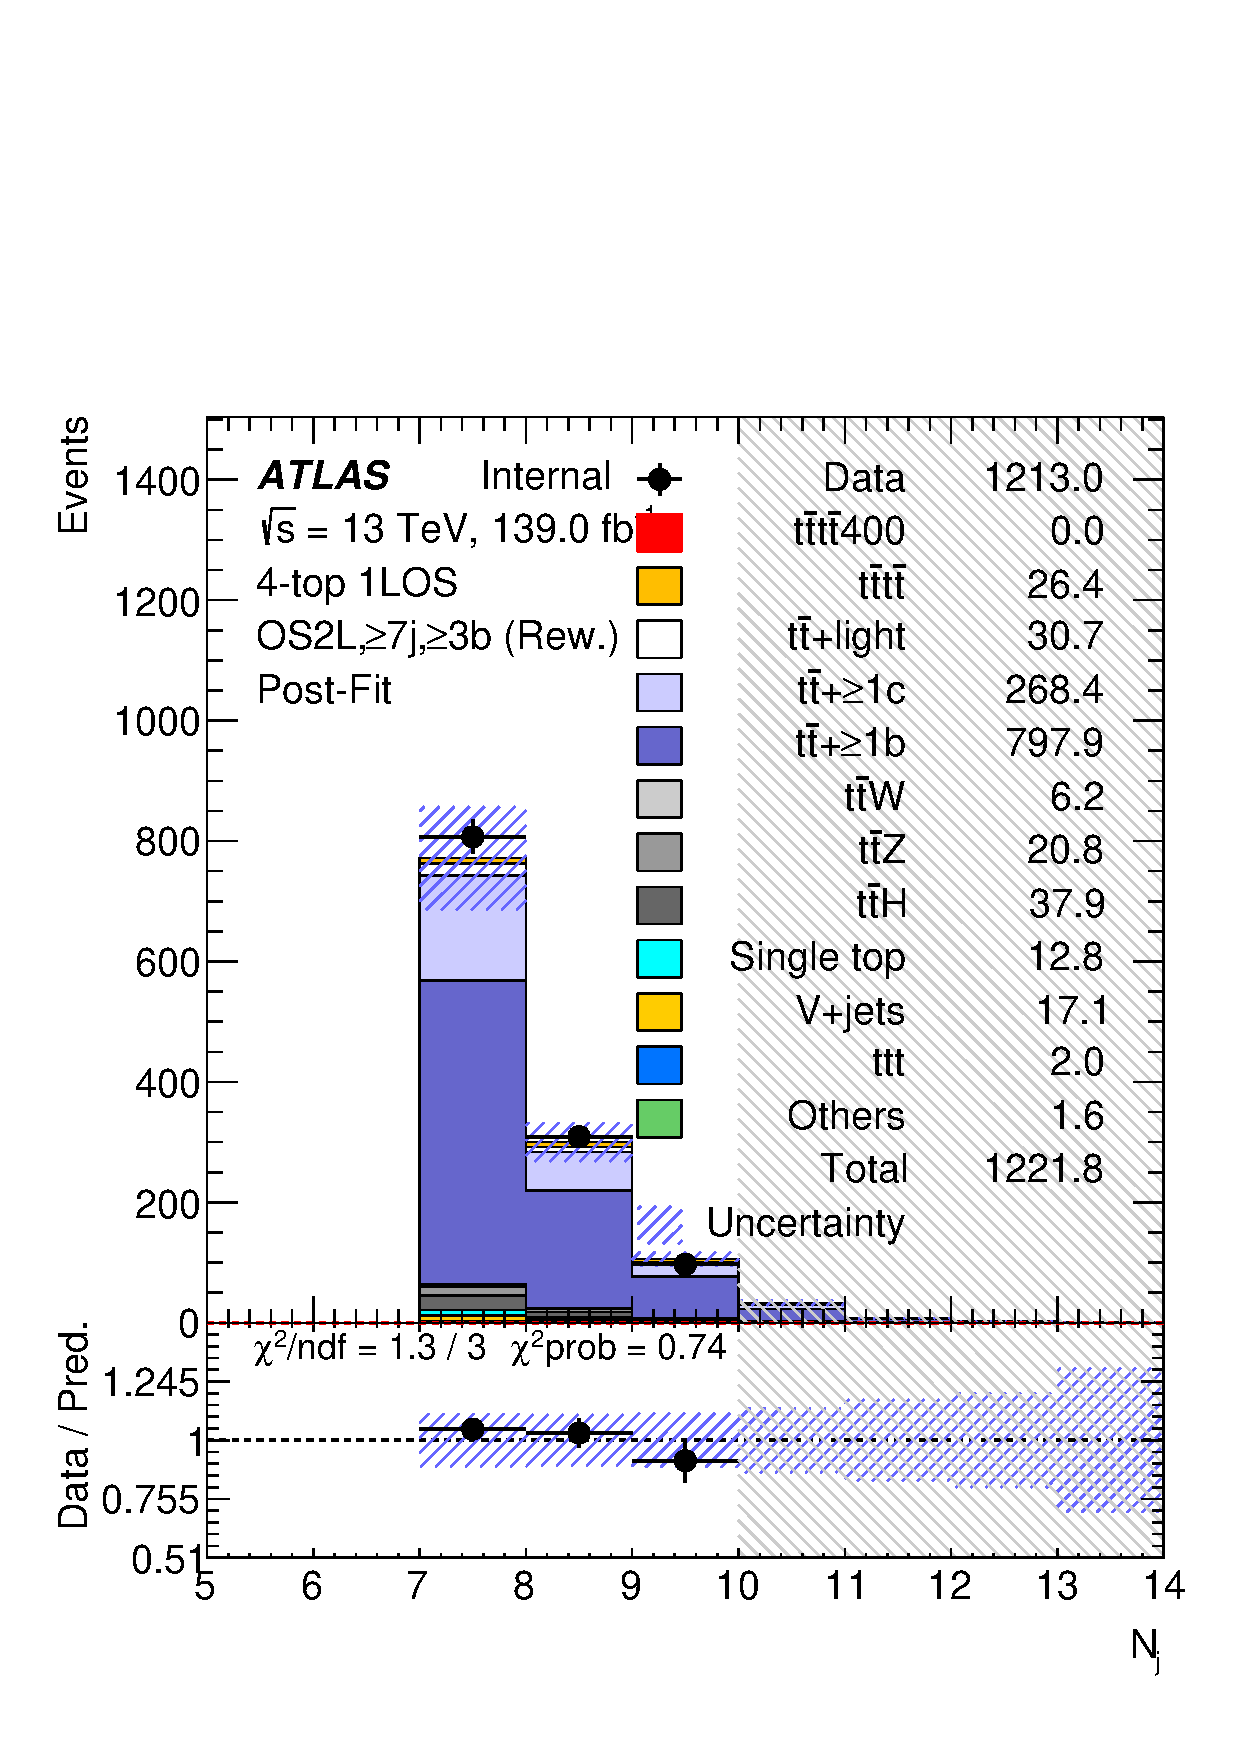
\includegraphics[width=0.3\textwidth]{figures/NNPlots/MVATrainRegion/Rew/os2l_ge7jge3b_nJets_postFit.pdf}
    \caption{nJets}
    \end{center}
    \end{subfigure}
    \caption{\label{fig:NNPlots_MVATrainReg_7} The comparison between variables pre-fit distribution before (left) and after (middle) the NN-reweighting  in 1L MVA training regions ($\geq 7j,\geq 3b$). The post-fit distribution after the NN-reweighting is shown on the left. Blinded regions are excluded.}
\end{figure}

\begin{figure}[htbp!]
    \begin{subfigure}[t]{1\textwidth}
    \begin{center}
    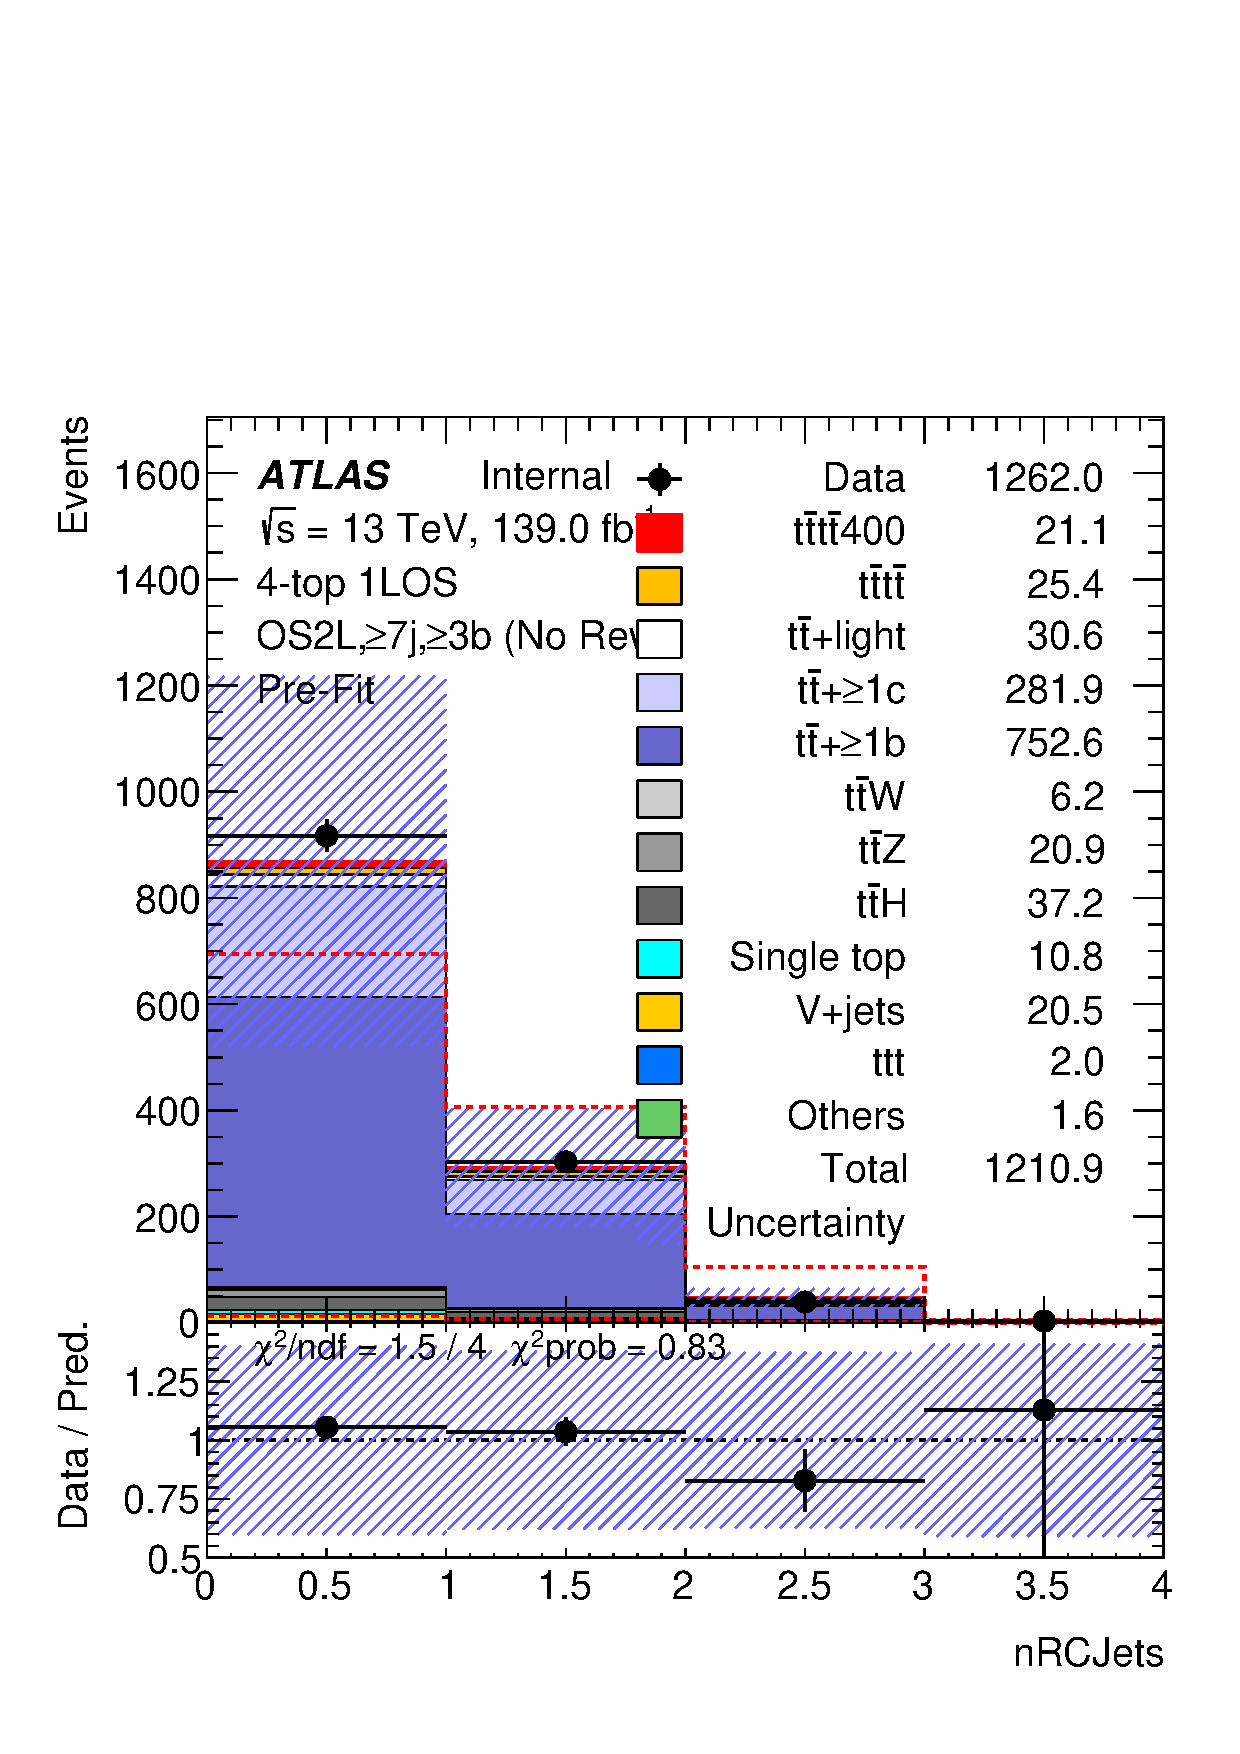
\includegraphics[width=0.3\textwidth]{figures/NNPlots/MVATrainRegion/NoRew/os2l_ge7jge3b_nRCJetsM100.pdf}
    
\includegraphics[width=0.3\textwidth]{figures/NNPlots/MVATrainRegion/Rew/os2l_ge7jge3b_nRCJetsM100.pdf}
    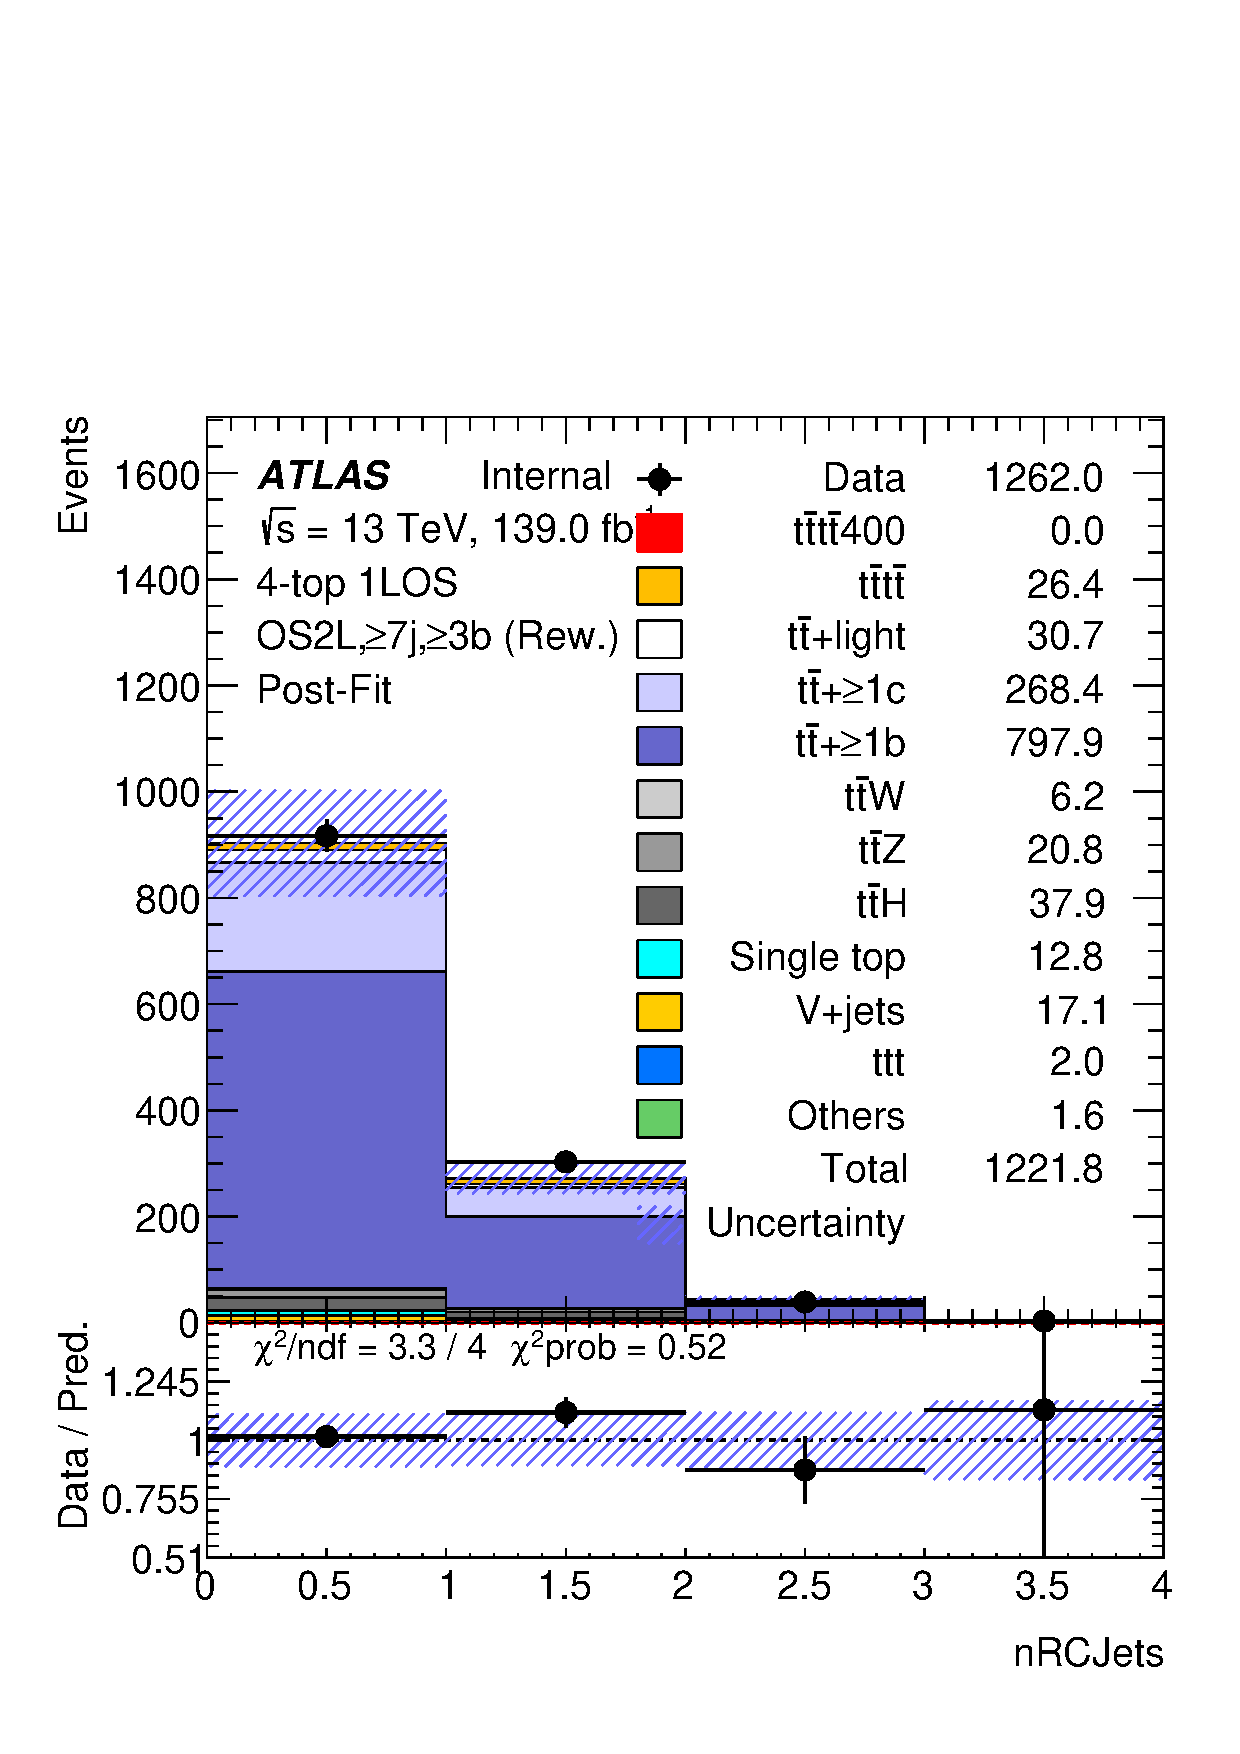
\includegraphics[width=0.3\textwidth]{figures/NNPlots/MVATrainRegion/Rew/os2l_ge7jge3b_nRCJetsM100_postFit.pdf}
    \caption{nRCJets}
    \end{center}
    \end{subfigure}

    \begin{subfigure}[t]{1\textwidth}
    \begin{center}
    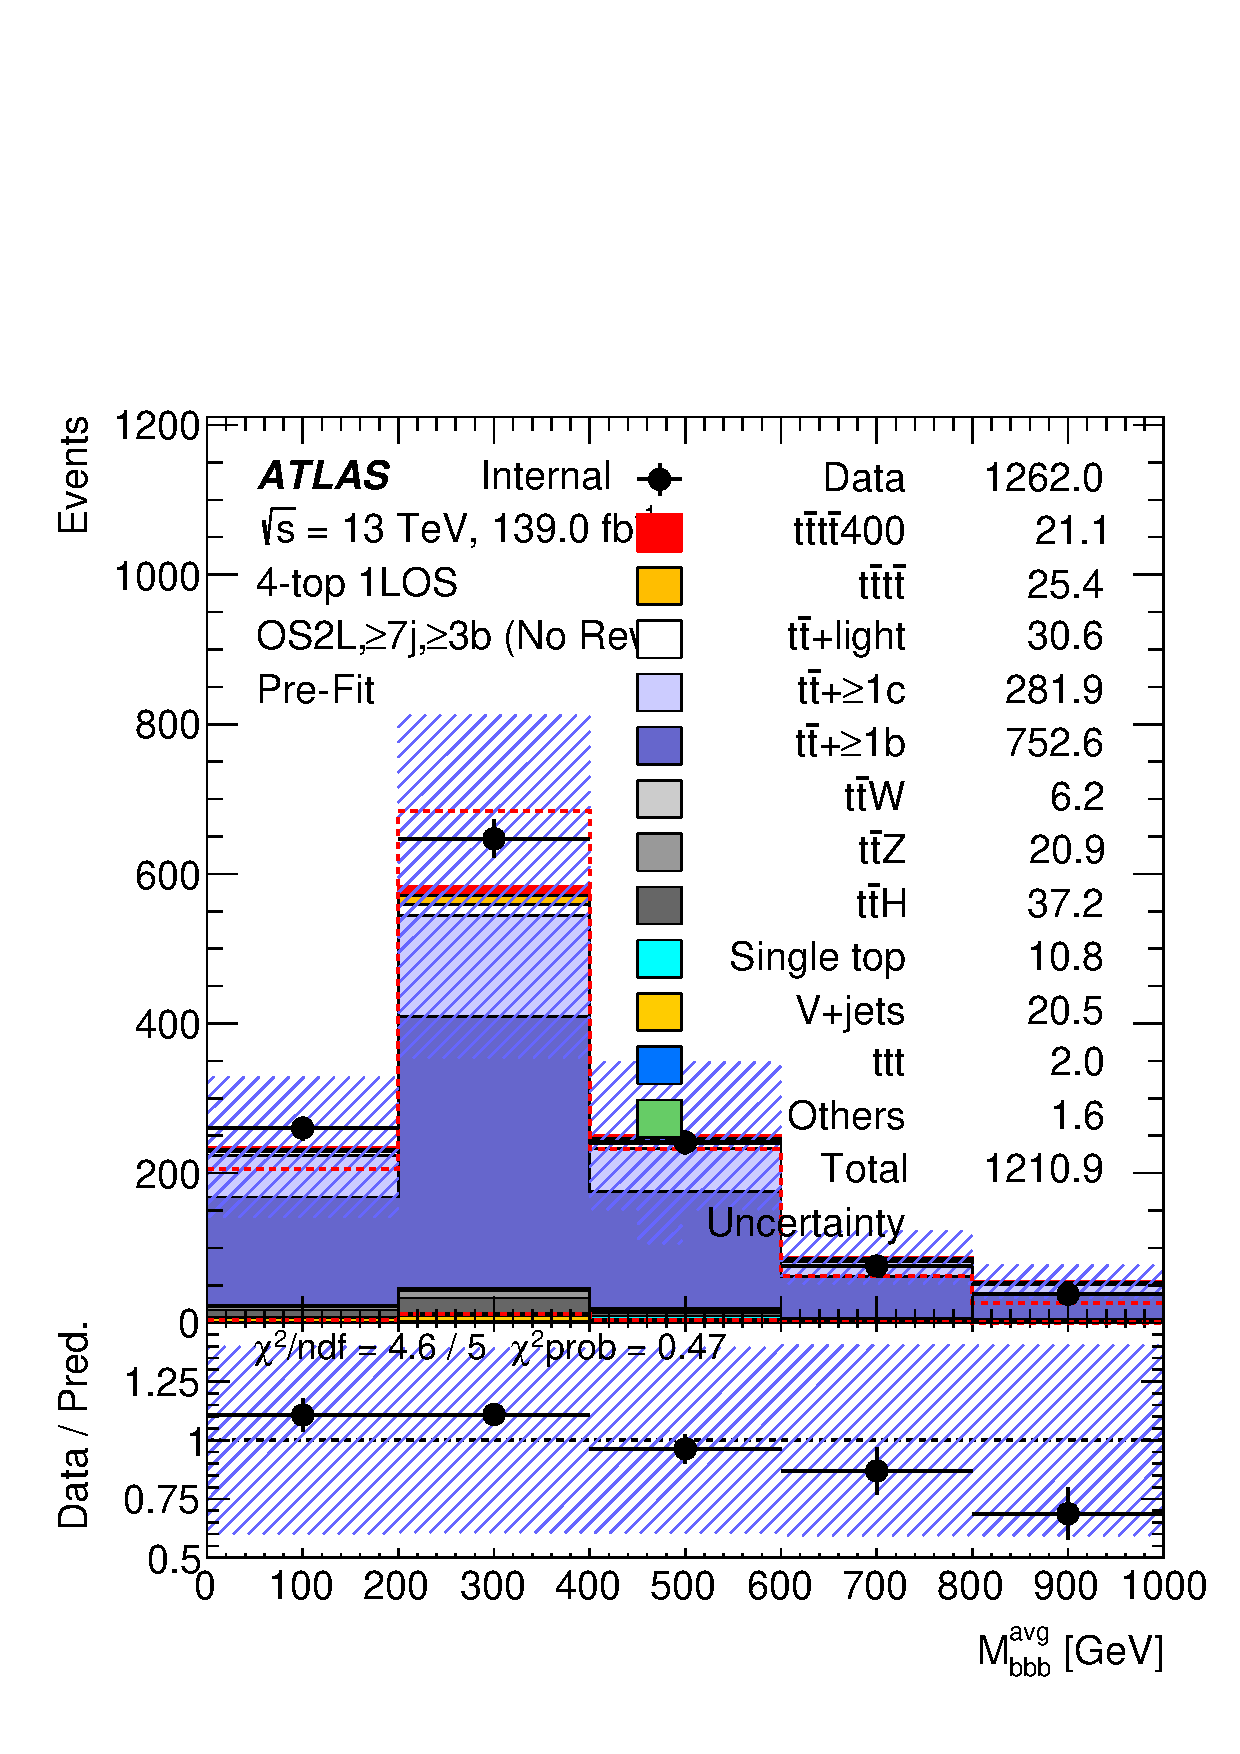
\includegraphics[width=0.3\textwidth]{figures/NNPlots/MVATrainRegion/NoRew/os2l_ge7jge3b_Mbbb_Avg_DL1r_70.pdf}
    
\includegraphics[width=0.3\textwidth]{figures/NNPlots/MVATrainRegion/Rew/os2l_ge7jge3b_Mbbb_Avg_DL1r_70.pdf}
    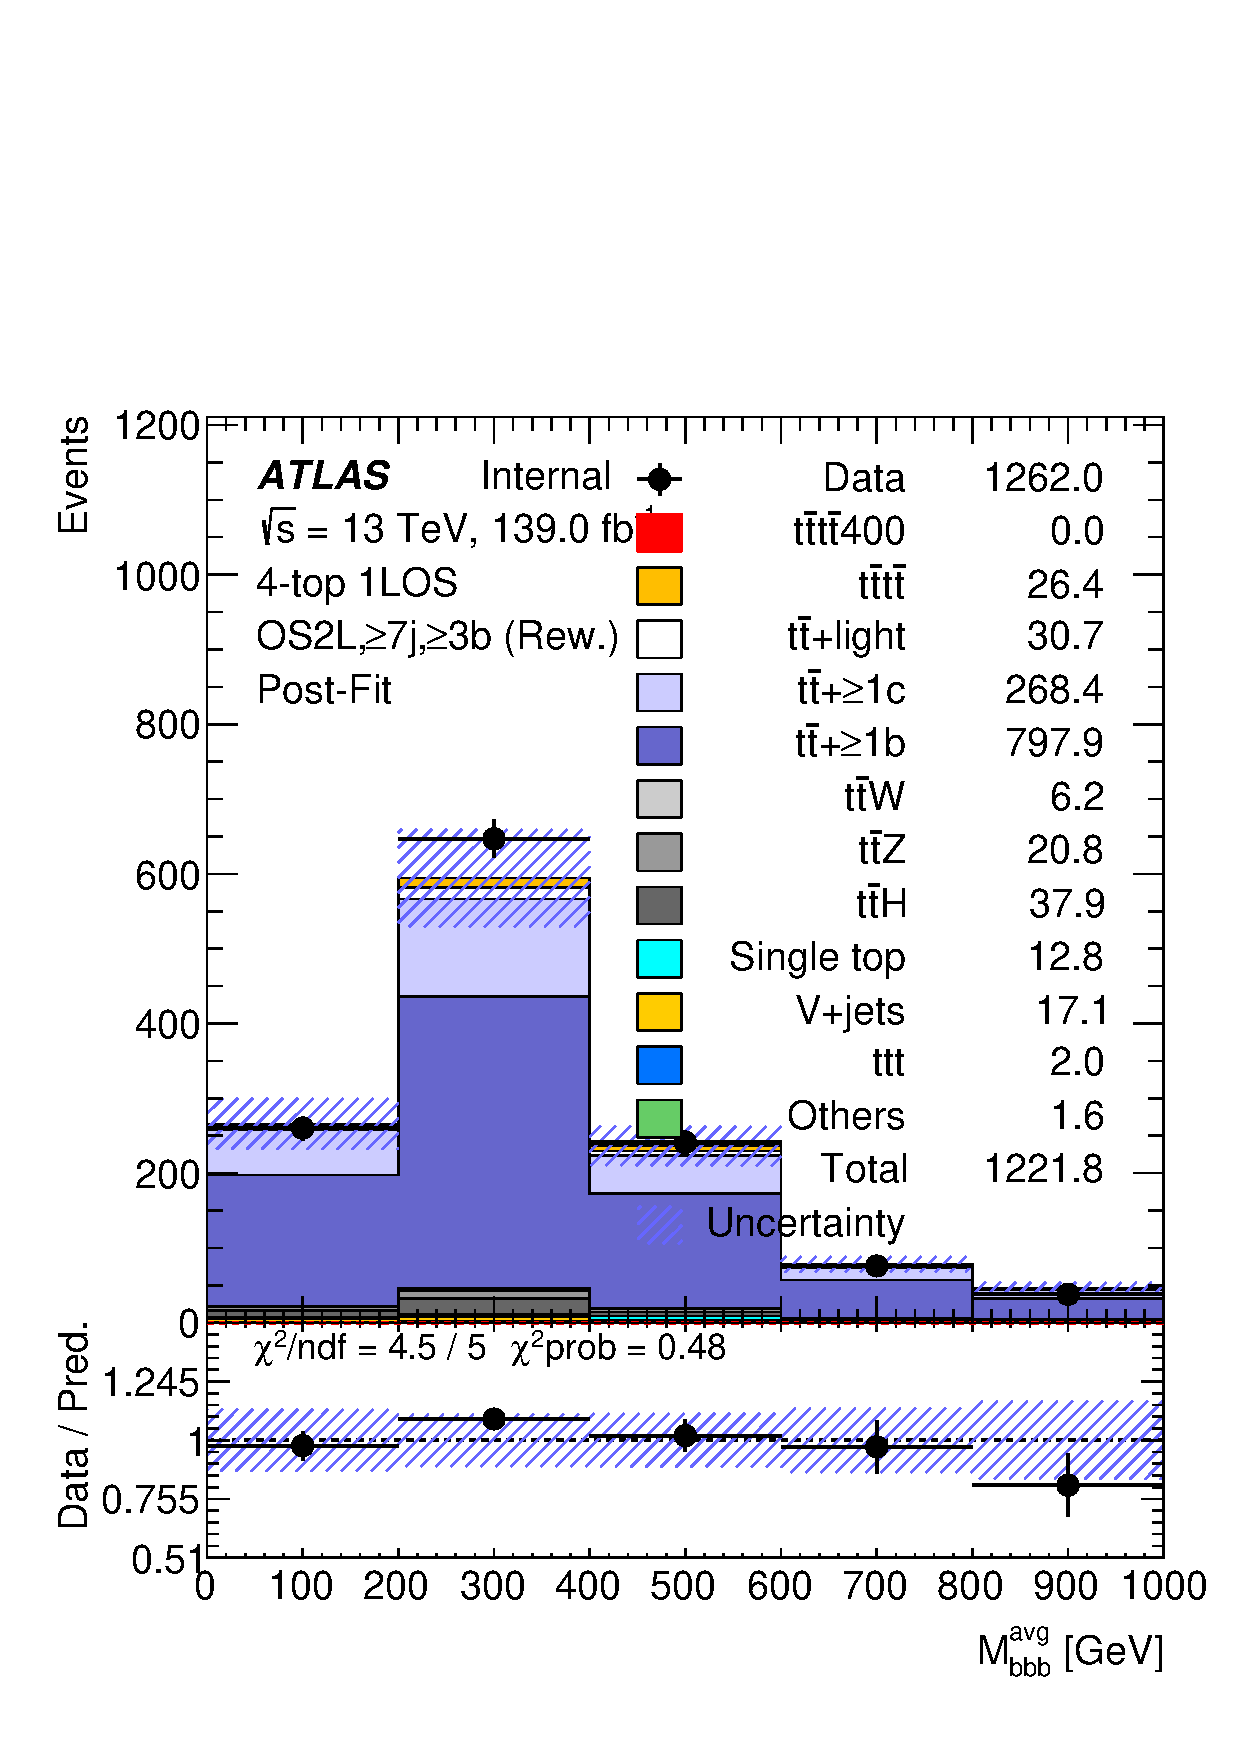
\includegraphics[width=0.3\textwidth]{figures/NNPlots/MVATrainRegion/Rew/os2l_ge7jge3b_Mbbb_Avg_DL1r_70_postFit.pdf}
    \caption{$M^{avg}_{bbb}$}
    \end{center}
    \end{subfigure}

    \begin{subfigure}[t]{1\textwidth}
    \begin{center}
    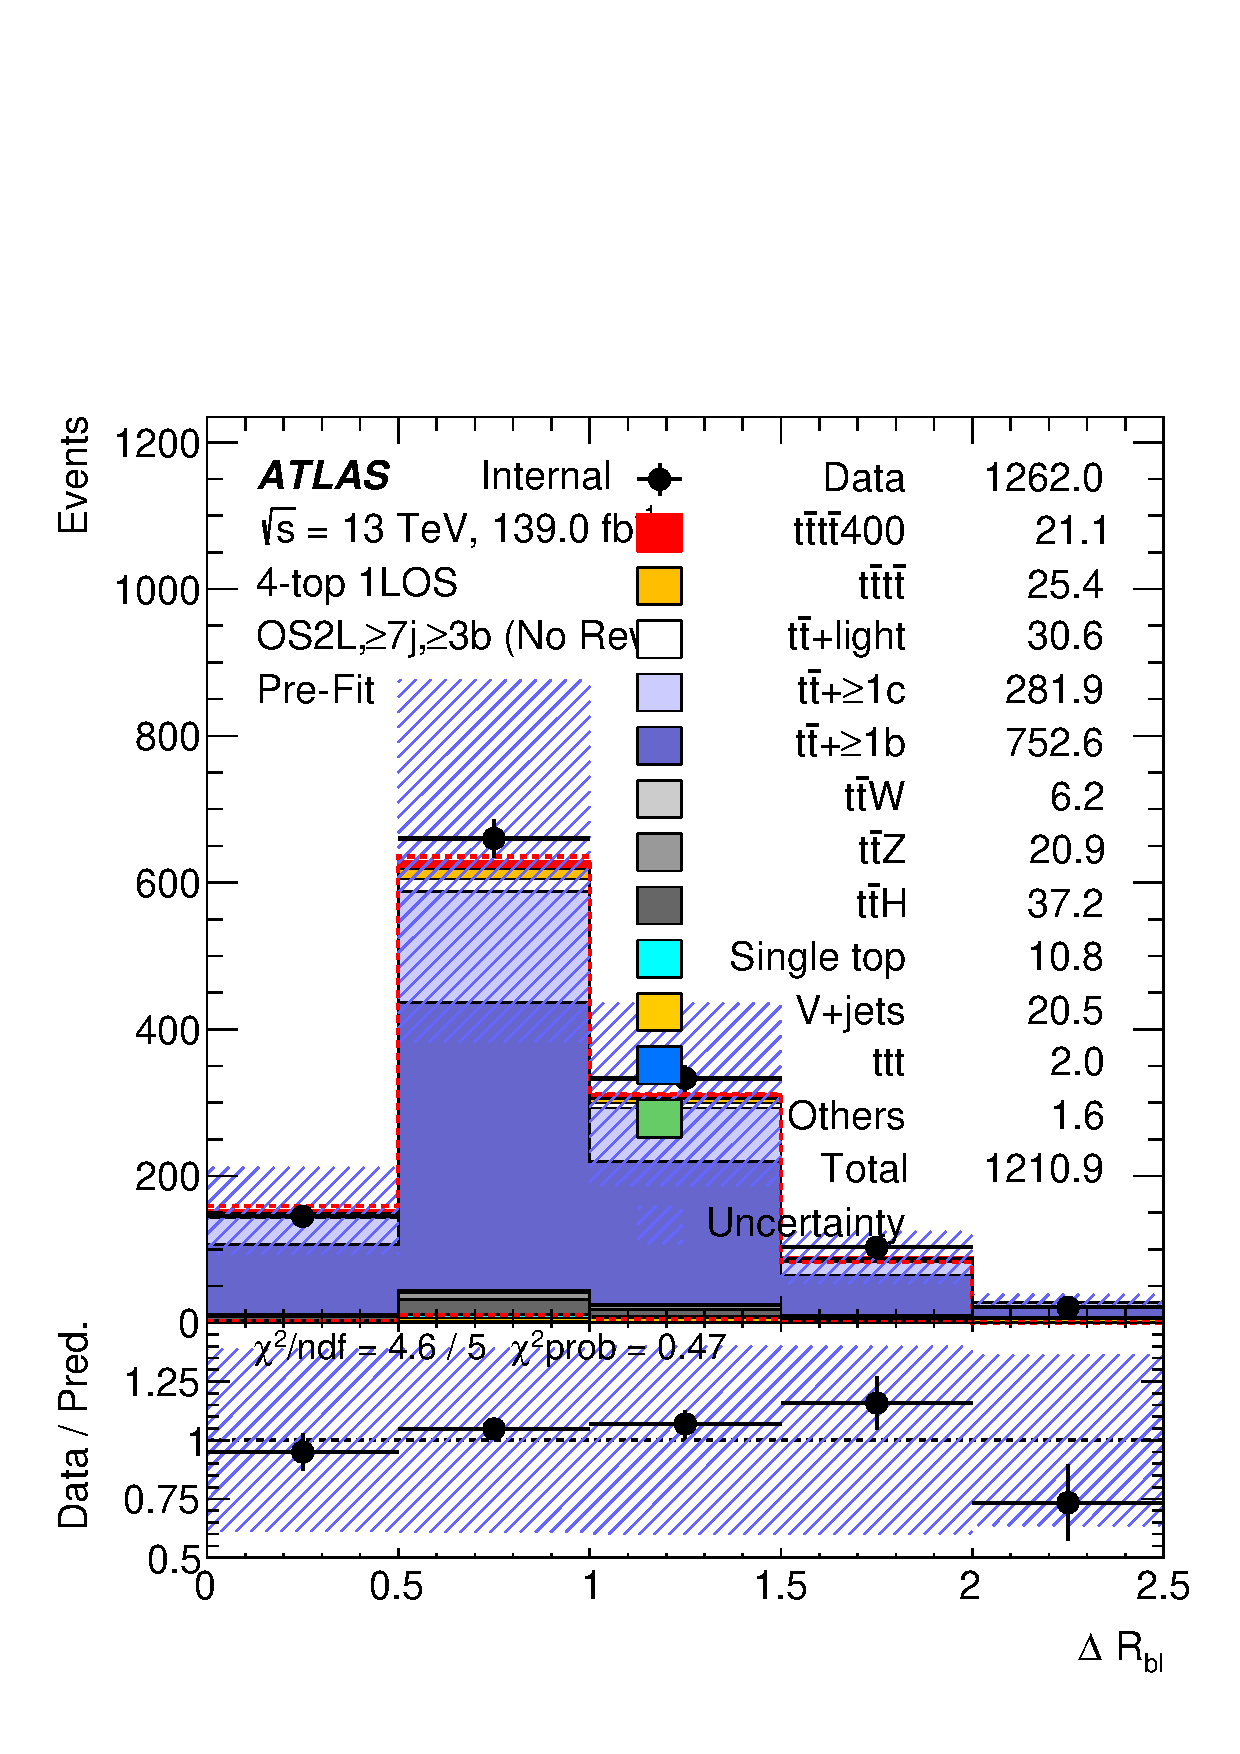
\includegraphics[width=0.3\textwidth]{figures/NNPlots/MVATrainRegion/NoRew/os2l_ge7jge3b_dRbl_MindR_DL1r_70.pdf}
    
\includegraphics[width=0.3\textwidth]{figures/NNPlots/MVATrainRegion/Rew/os2l_ge7jge3b_dRbl_MindR_DL1r_70.pdf}
    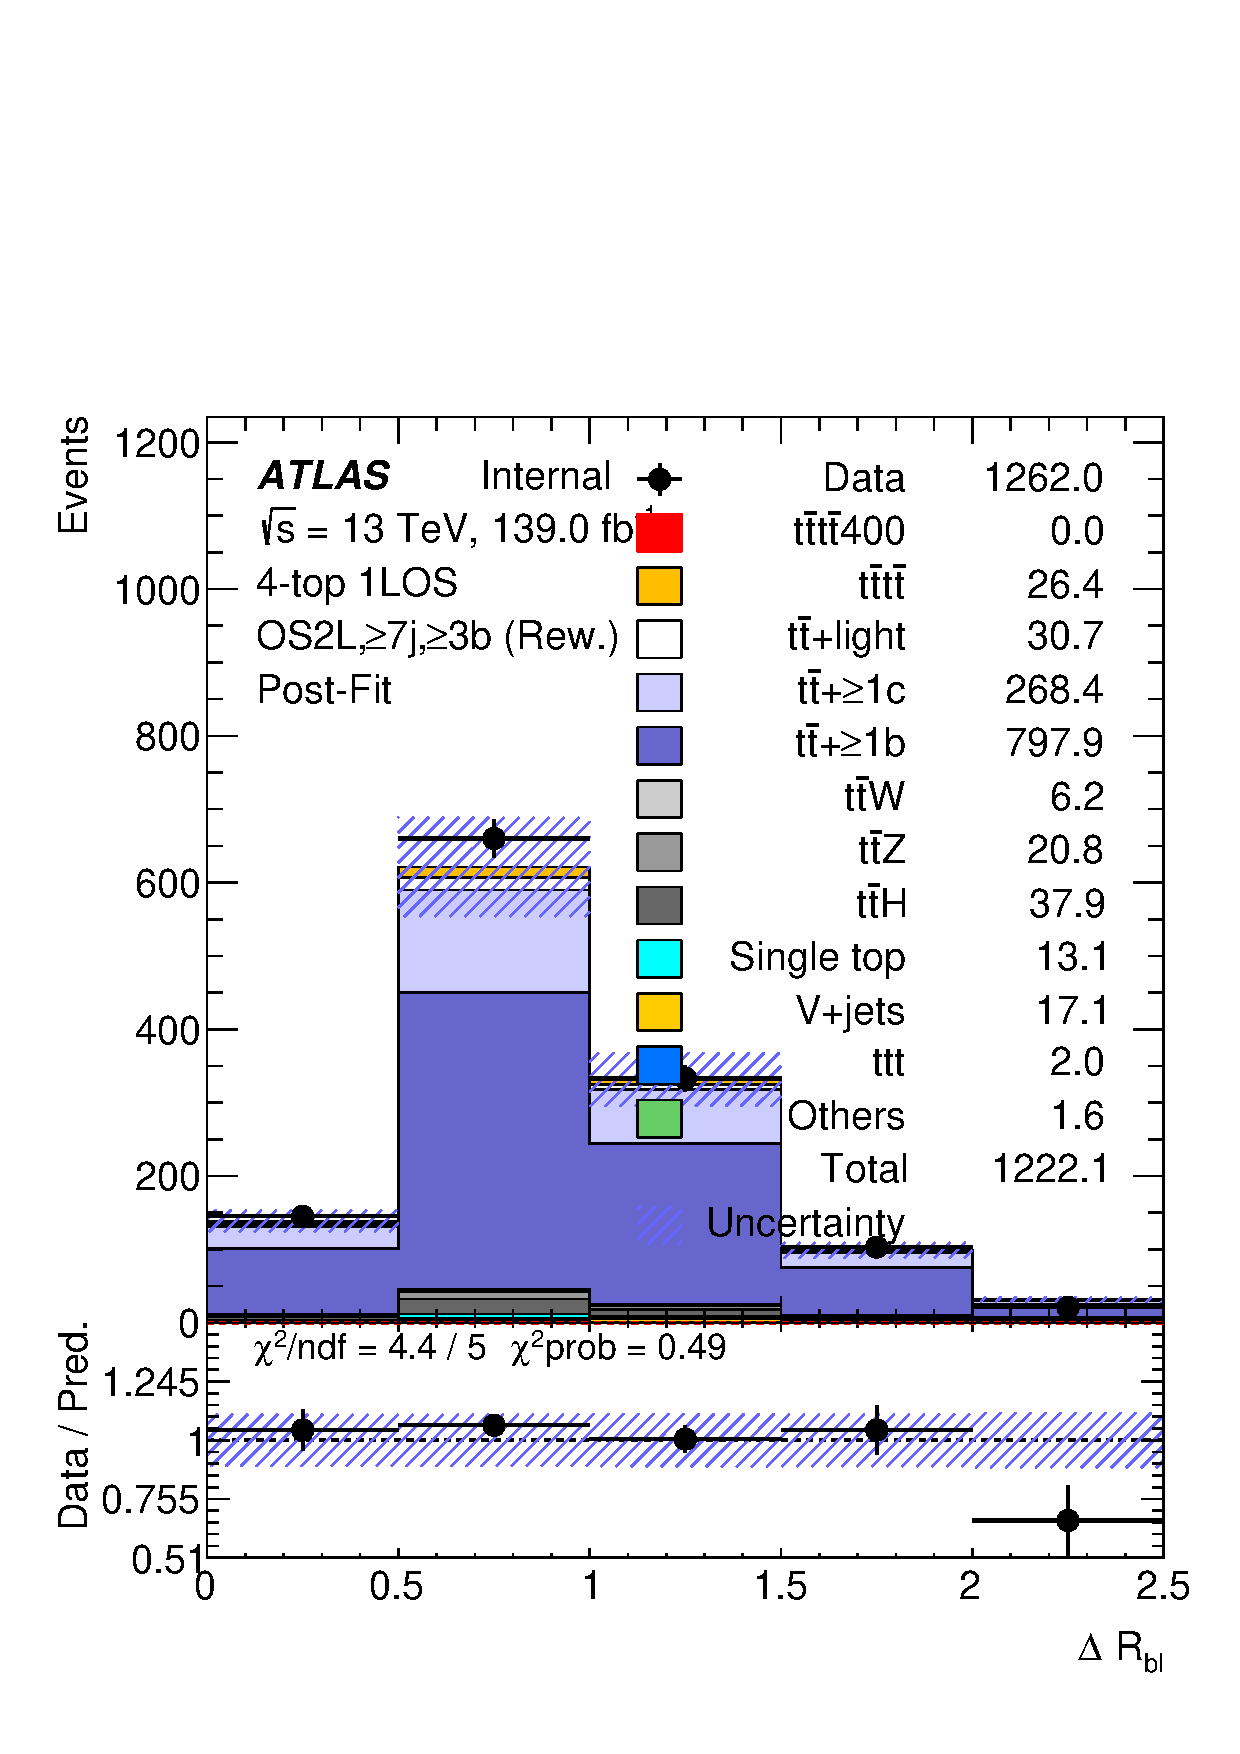
\includegraphics[width=0.3\textwidth]{figures/NNPlots/MVATrainRegion/Rew/os2l_ge7jge3b_dRbl_MindR_DL1r_70_postFit.pdf}
    \caption{$\Delta R^{min}_{bl}$}
    \end{center}
    \end{subfigure}
    \caption{\label{fig:NNPlots_MVATrainReg_8} The comparison between variables pre-fit distribution before (left) and after (middle) the NN-reweighting  in 1L MVA training regions ($\geq 7j,\geq 3b$). The post-fit distribution after the NN-reweighting is shown on the left. Blinded regions are excluded.}
\end{figure}

\begin{figure}[htbp!]
    \begin{subfigure}[t]{1\textwidth}
    \begin{center}
    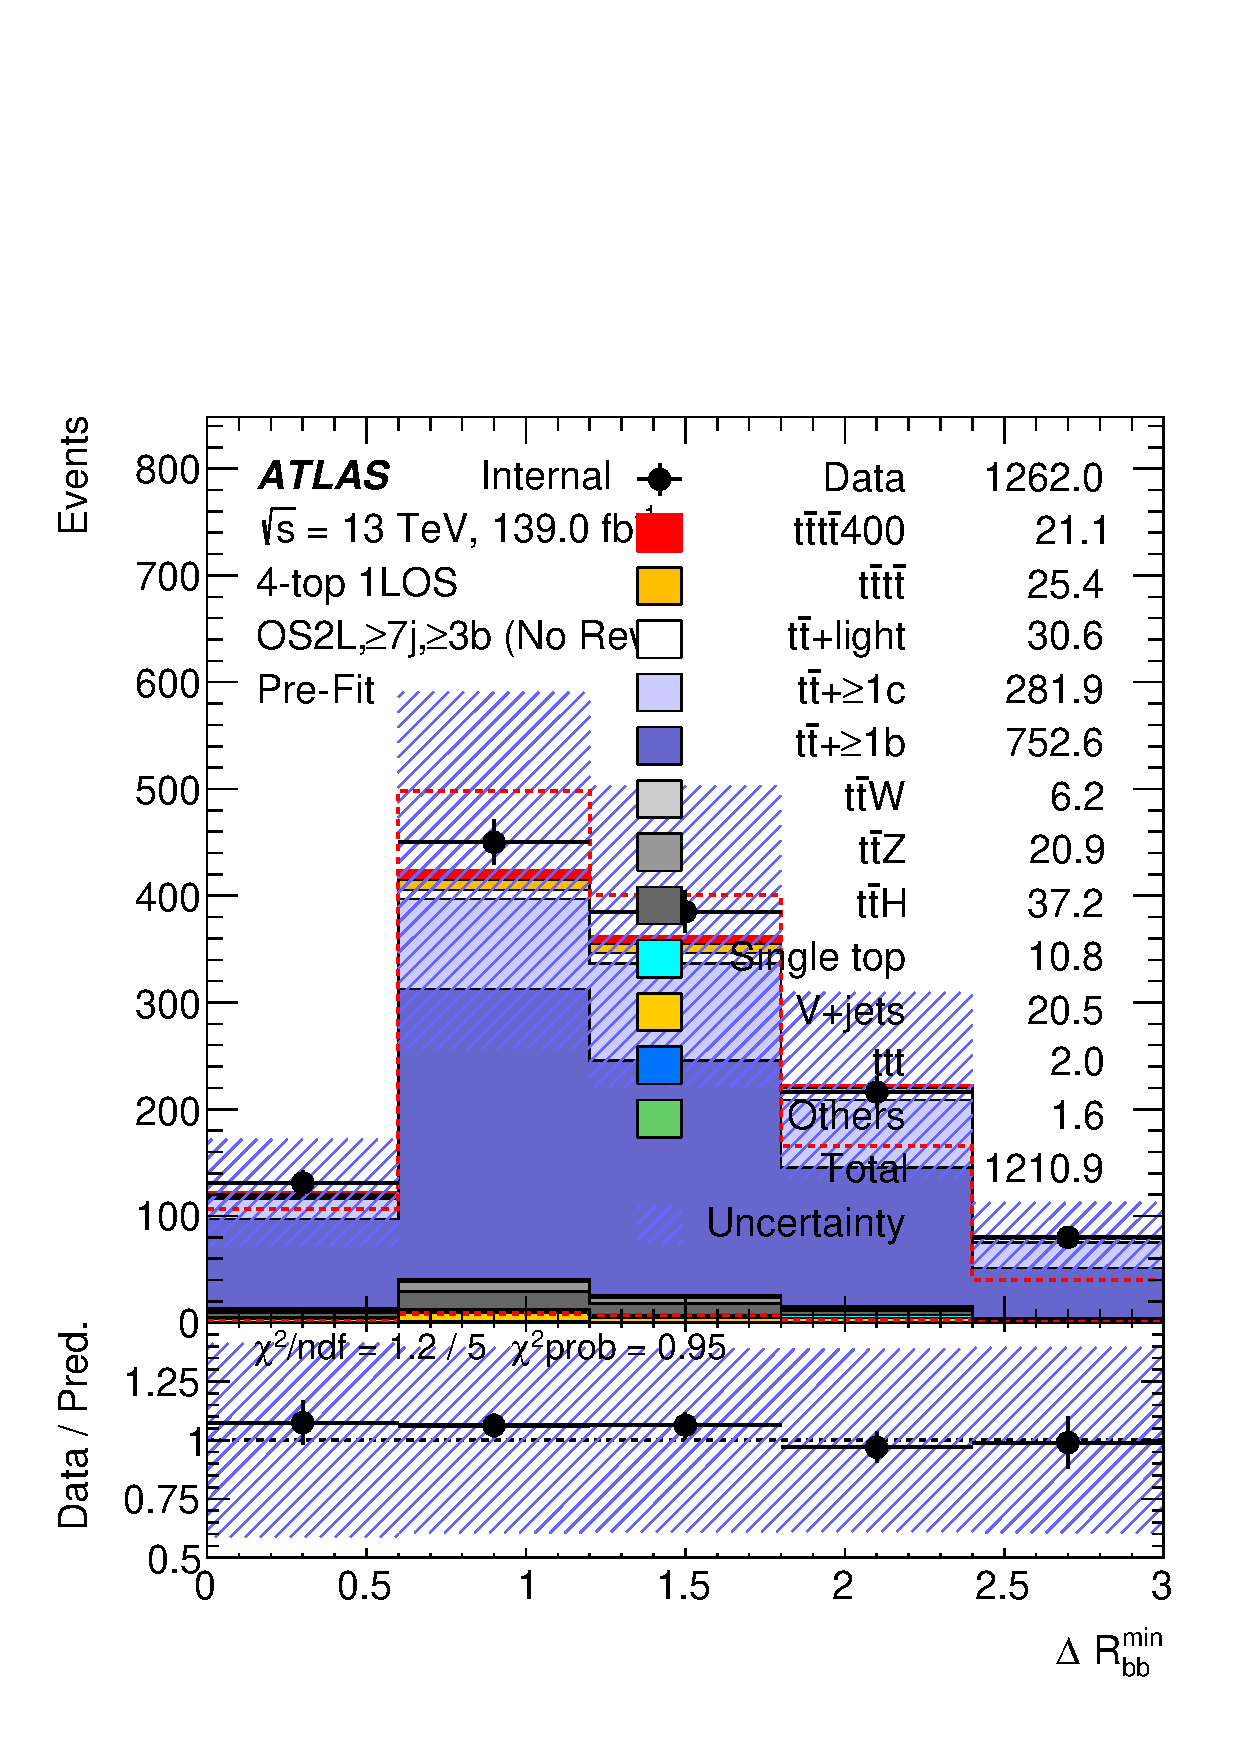
\includegraphics[width=0.3\textwidth]{figures/NNPlots/MVATrainRegion/NoRew/os2l_ge7jge3b_dRbb_MindR_DL1r_70.pdf}
    
\includegraphics[width=0.3\textwidth]{figures/NNPlots/MVATrainRegion/Rew/os2l_ge7jge3b_dRbb_MindR_DL1r_70.pdf}
    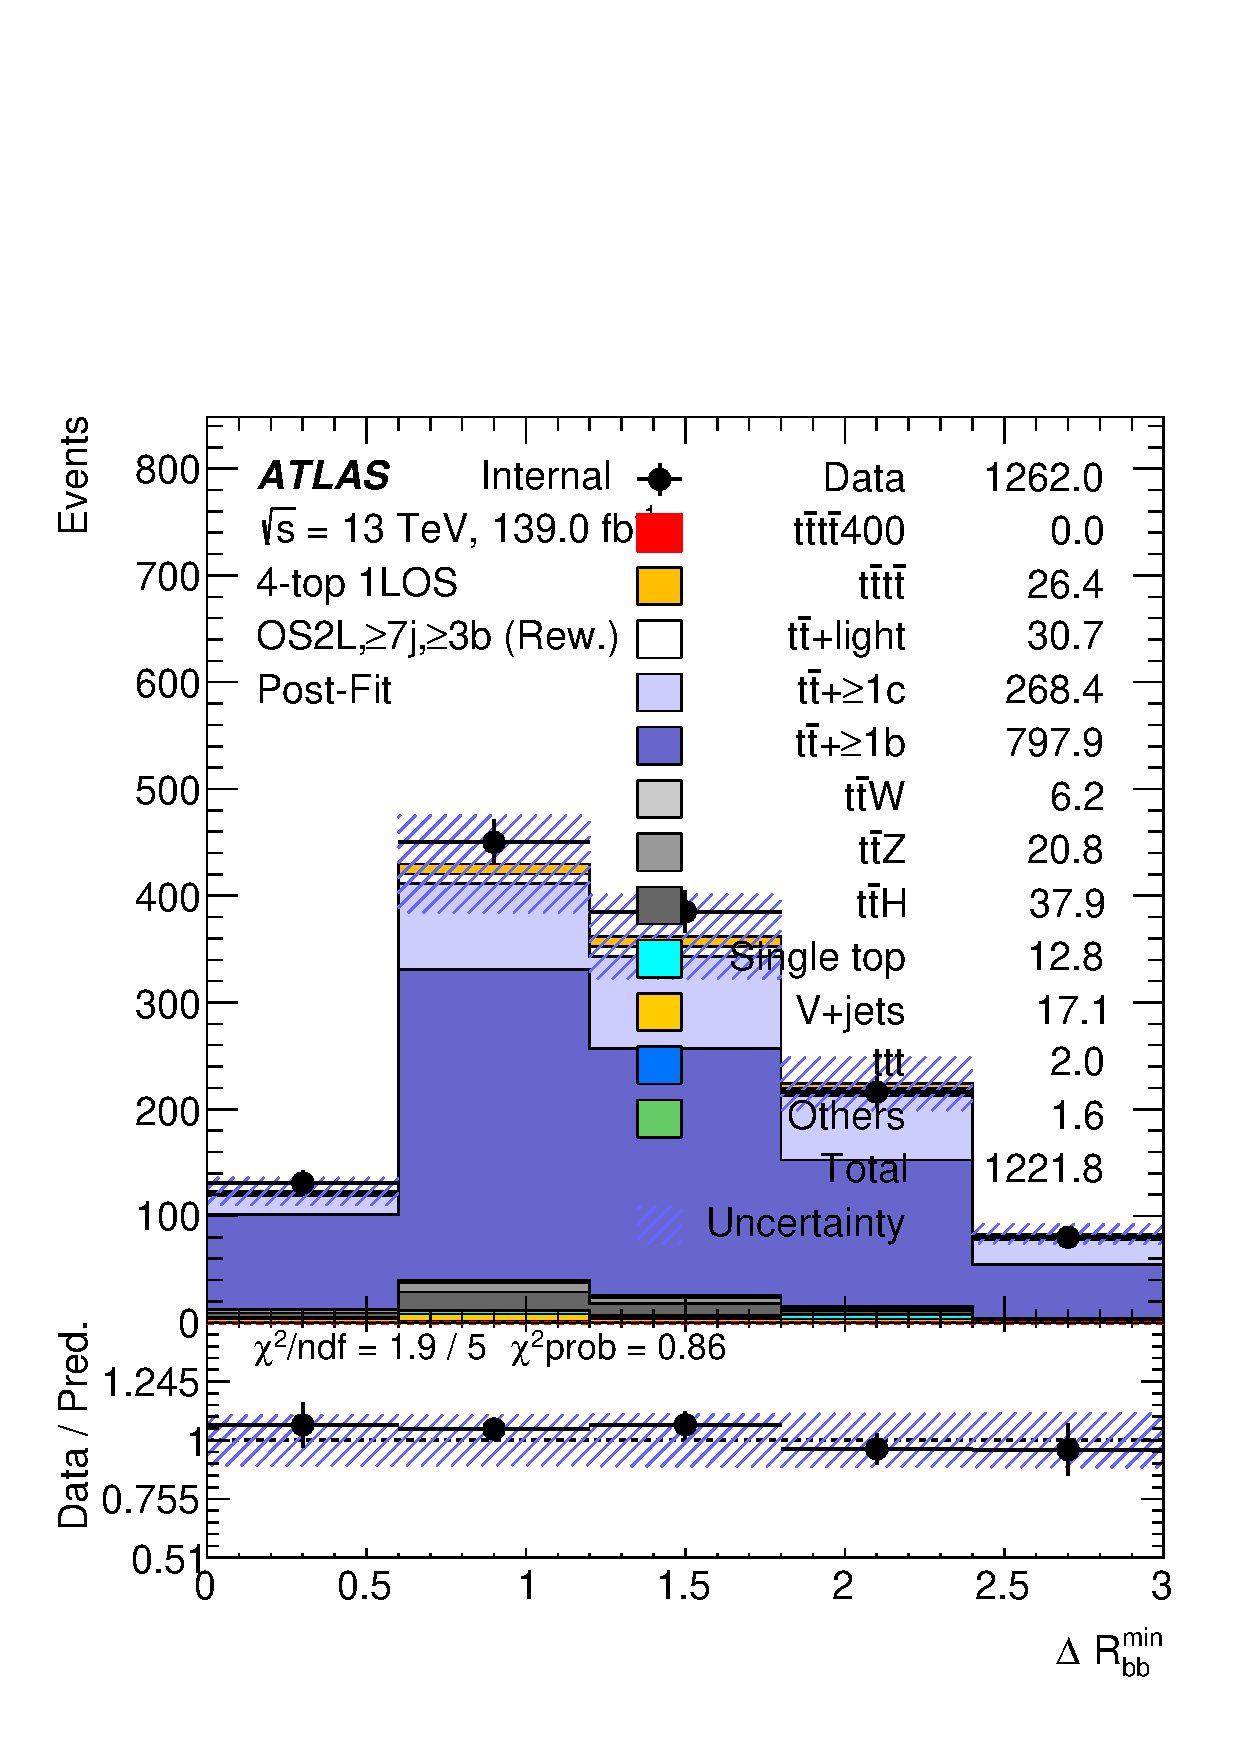
\includegraphics[width=0.3\textwidth]{figures/NNPlots/MVATrainRegion/Rew/os2l_ge7jge3b_dRbb_MindR_DL1r_70_postFit.pdf}
    \caption{$\Delta R^{min}_{bb}$}
    \end{center}
    \end{subfigure}

    \begin{subfigure}[t]{1\textwidth}
    \begin{center}
    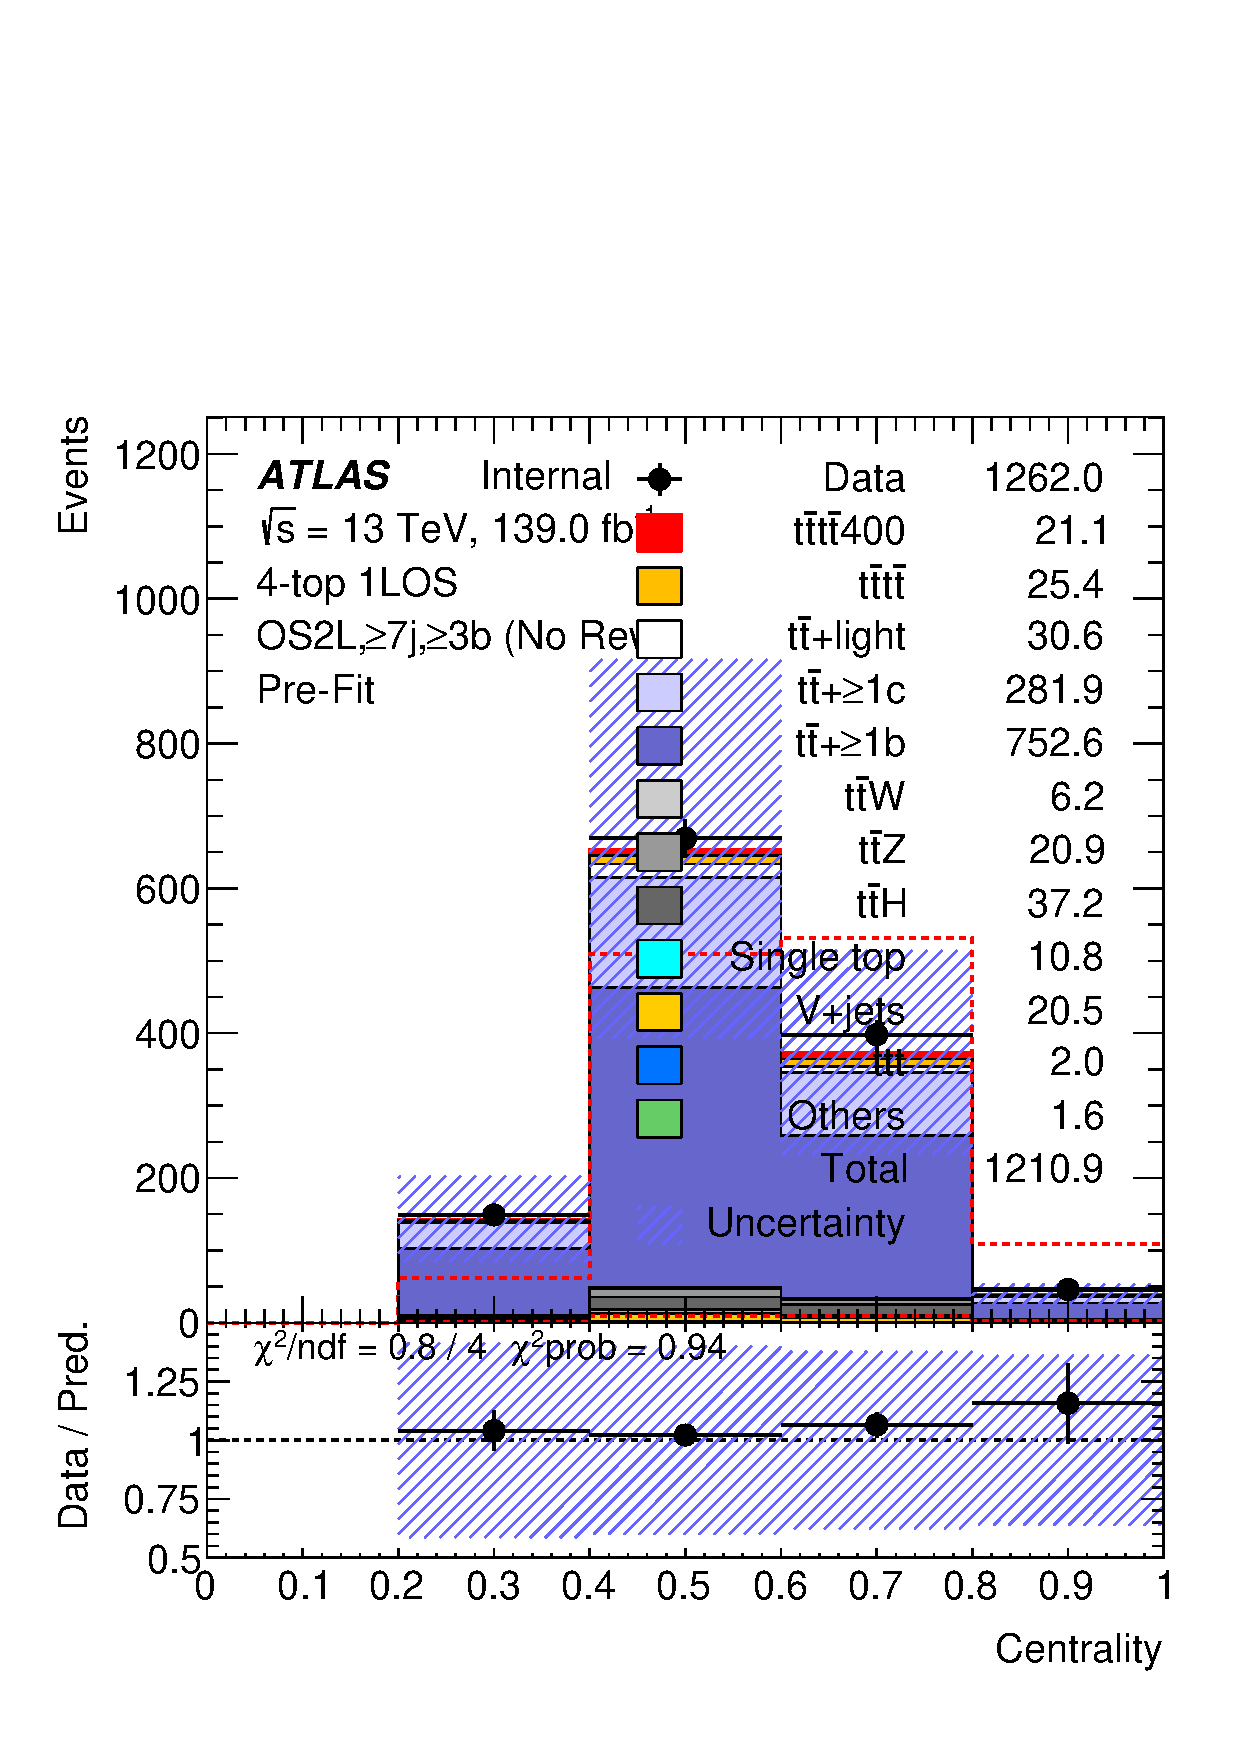
\includegraphics[width=0.3\textwidth]{figures/NNPlots/MVATrainRegion/NoRew/os2l_ge7jge3b_Centrality_all.pdf}
    
\includegraphics[width=0.3\textwidth]{figures/NNPlots/MVATrainRegion/Rew/os2l_ge7jge3b_Centrality_all.pdf}
    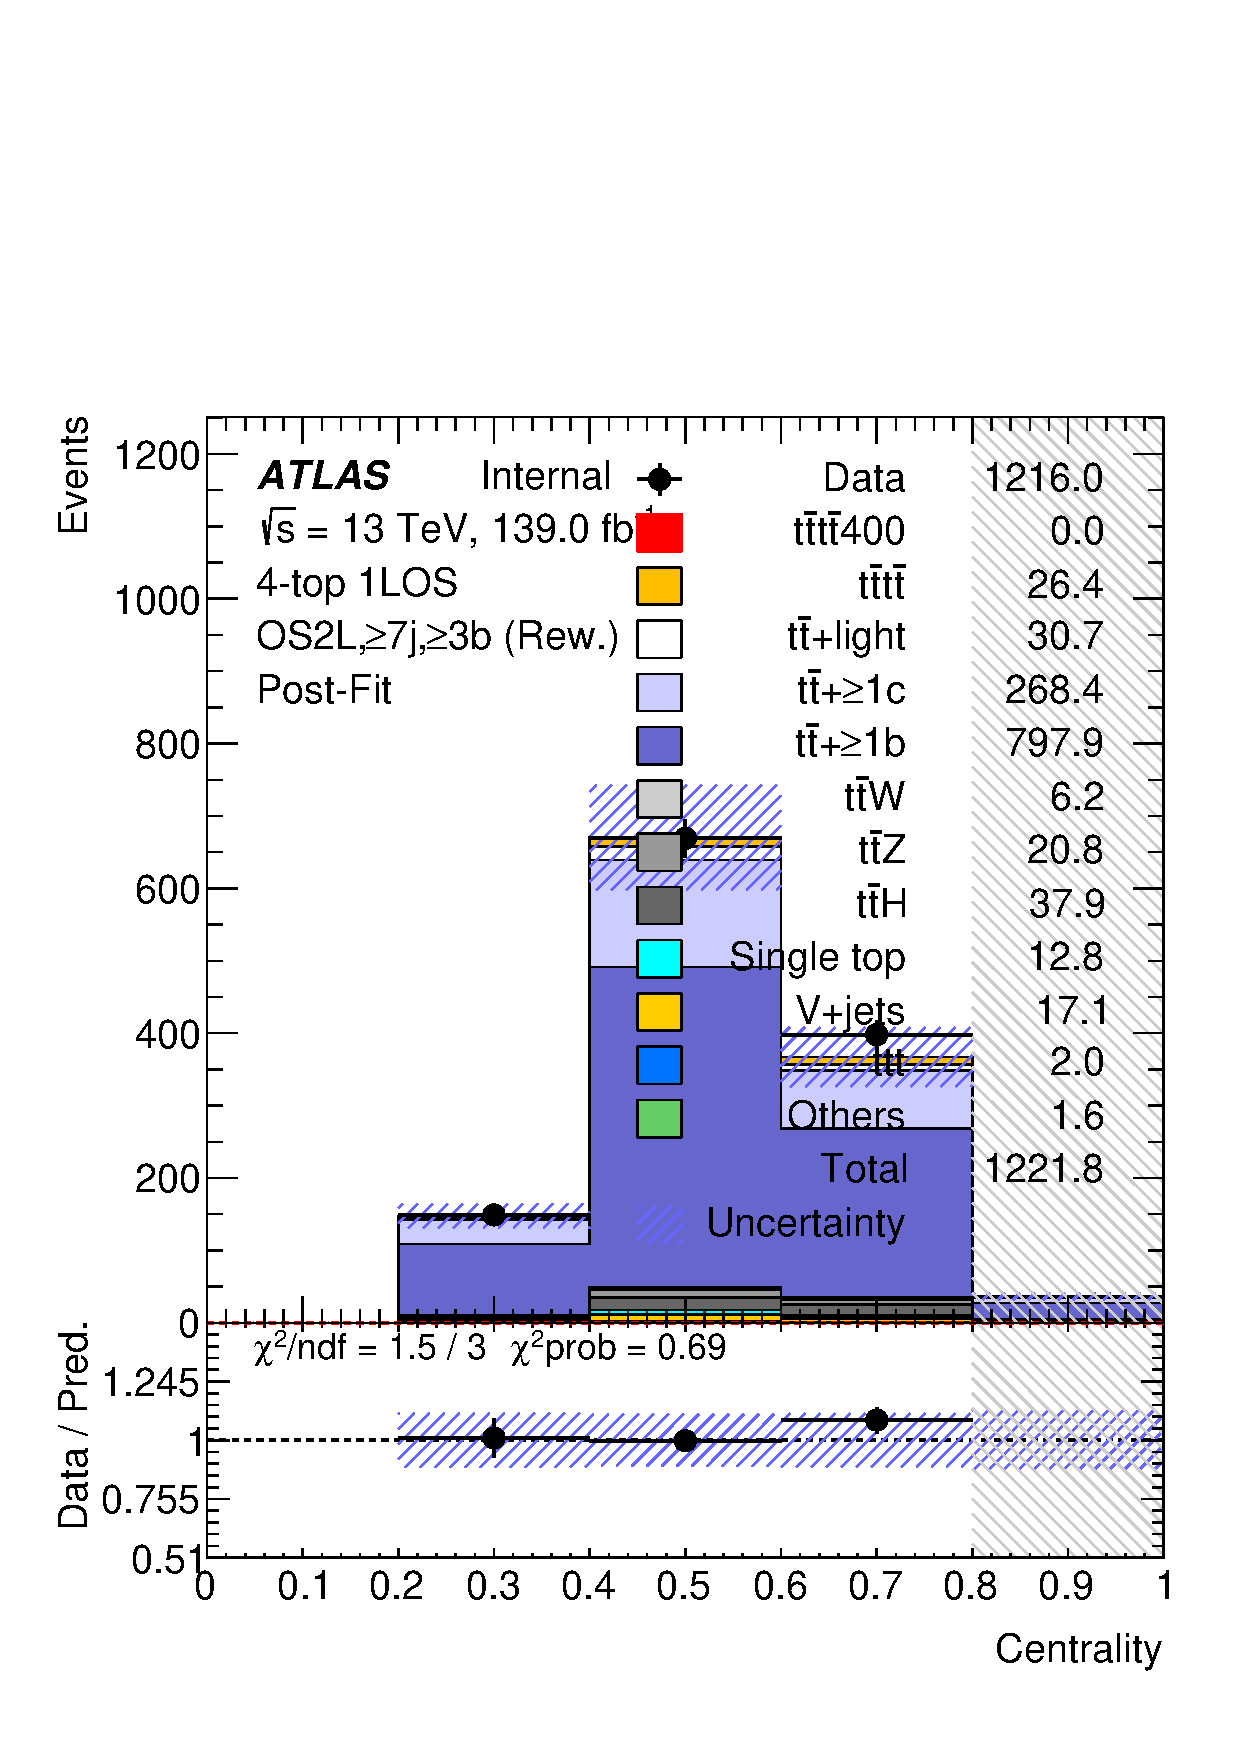
\includegraphics[width=0.3\textwidth]{figures/NNPlots/MVATrainRegion/Rew/os2l_ge7jge3b_Centrality_all_postFit.pdf}
    \caption{Centrality}
    \end{center}
    \end{subfigure}

    \begin{subfigure}[t]{1\textwidth}
    \begin{center}
    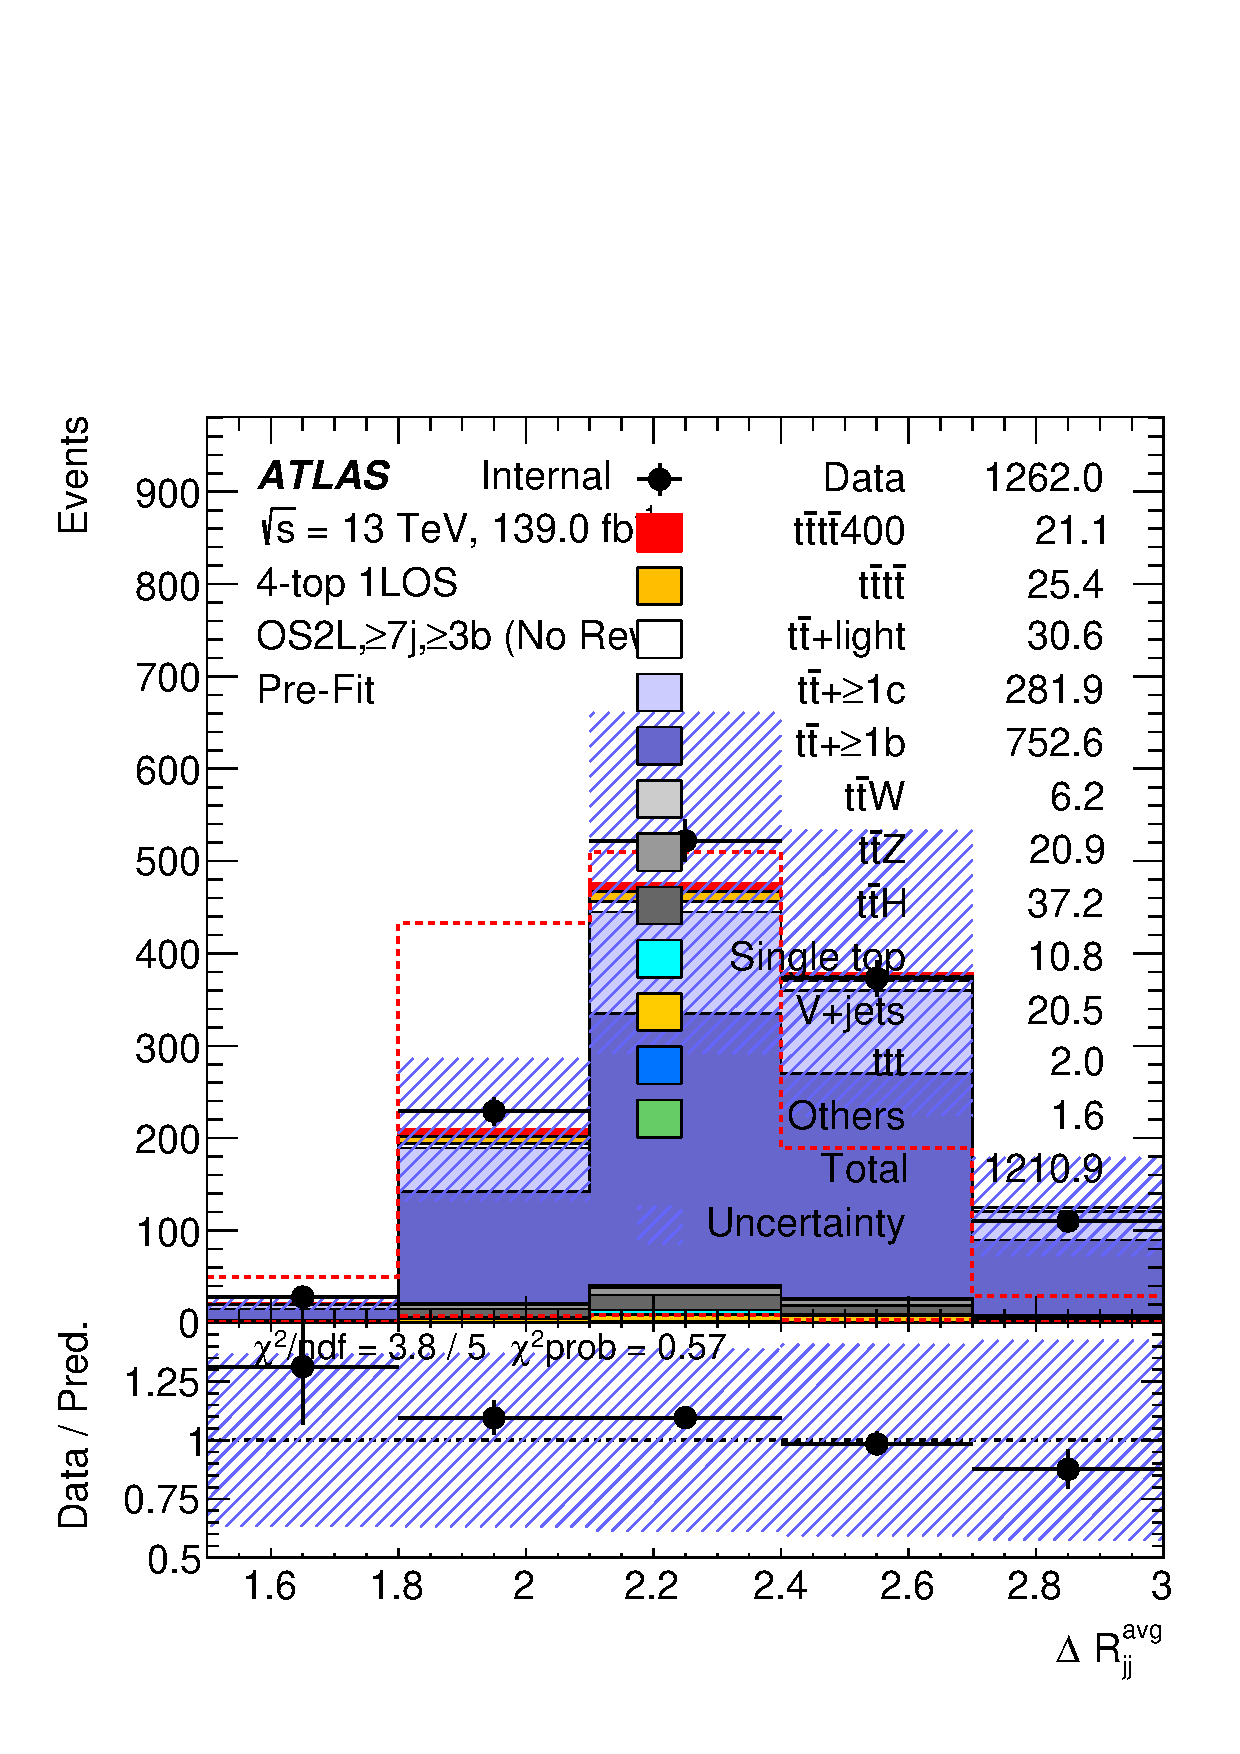
\includegraphics[width=0.3\textwidth]{figures/NNPlots/MVATrainRegion/NoRew/os2l_ge7jge3b_dRjj_Avg.pdf}
    
\includegraphics[width=0.3\textwidth]{figures/NNPlots/MVATrainRegion/Rew/os2l_ge7jge3b_dRjj_Avg.pdf}
    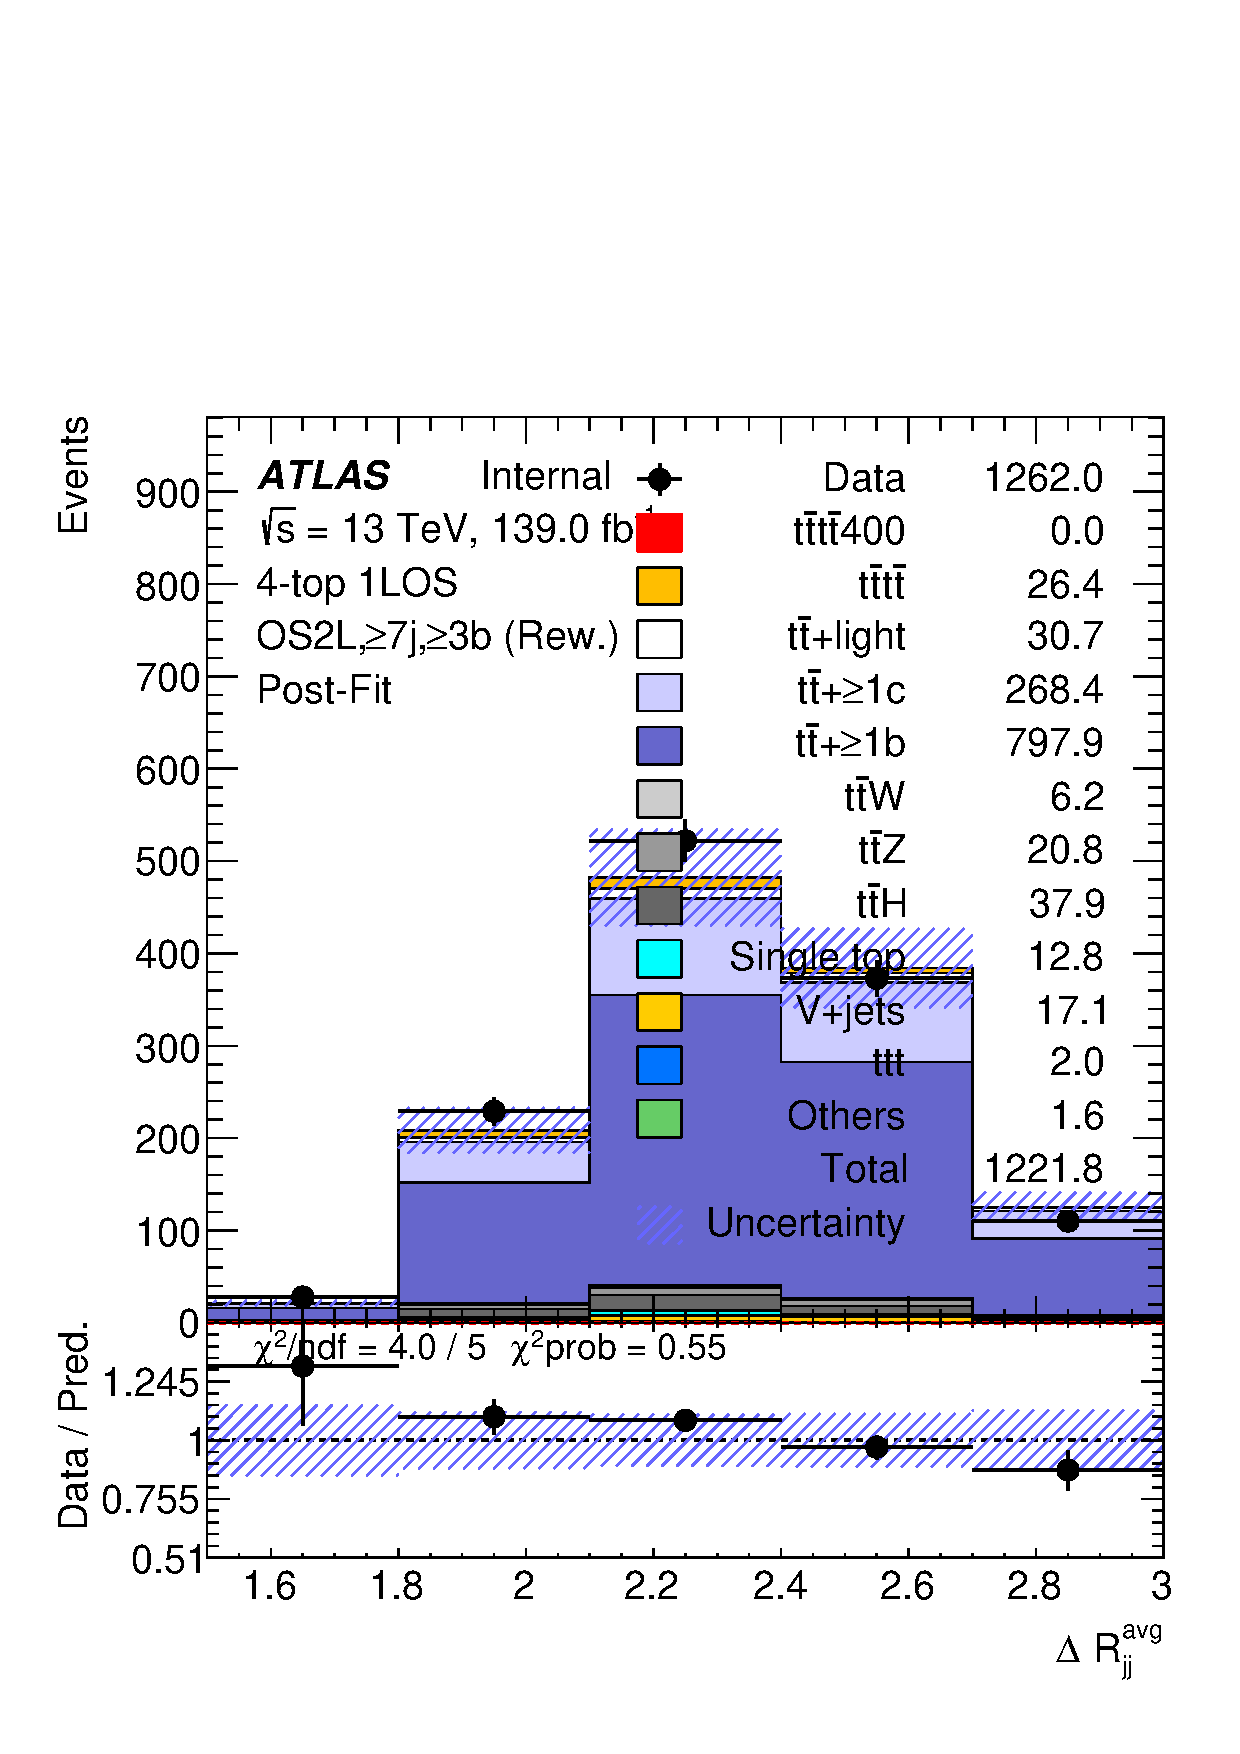
\includegraphics[width=0.3\textwidth]{figures/NNPlots/MVATrainRegion/Rew/os2l_ge7jge3b_dRjj_Avg_postFit.pdf}
    \caption{$\Delta R^{avg}_{jj}$}
    \end{center}
    \end{subfigure}
    \caption{\label{fig:NNPlots_MVATrainReg_9} The comparison between variables pre-fit distribution before (left) and after (middle) the NN-reweighting  in 1L MVA training regions ($\geq 7j,\geq 3b$). The post-fit distribution after the NN-reweighting is shown on the left. Blinded regions are excluded.}
\end{figure}

\begin{figure}[htbp!]
    \begin{subfigure}[t]{1\textwidth}
    \begin{center}
    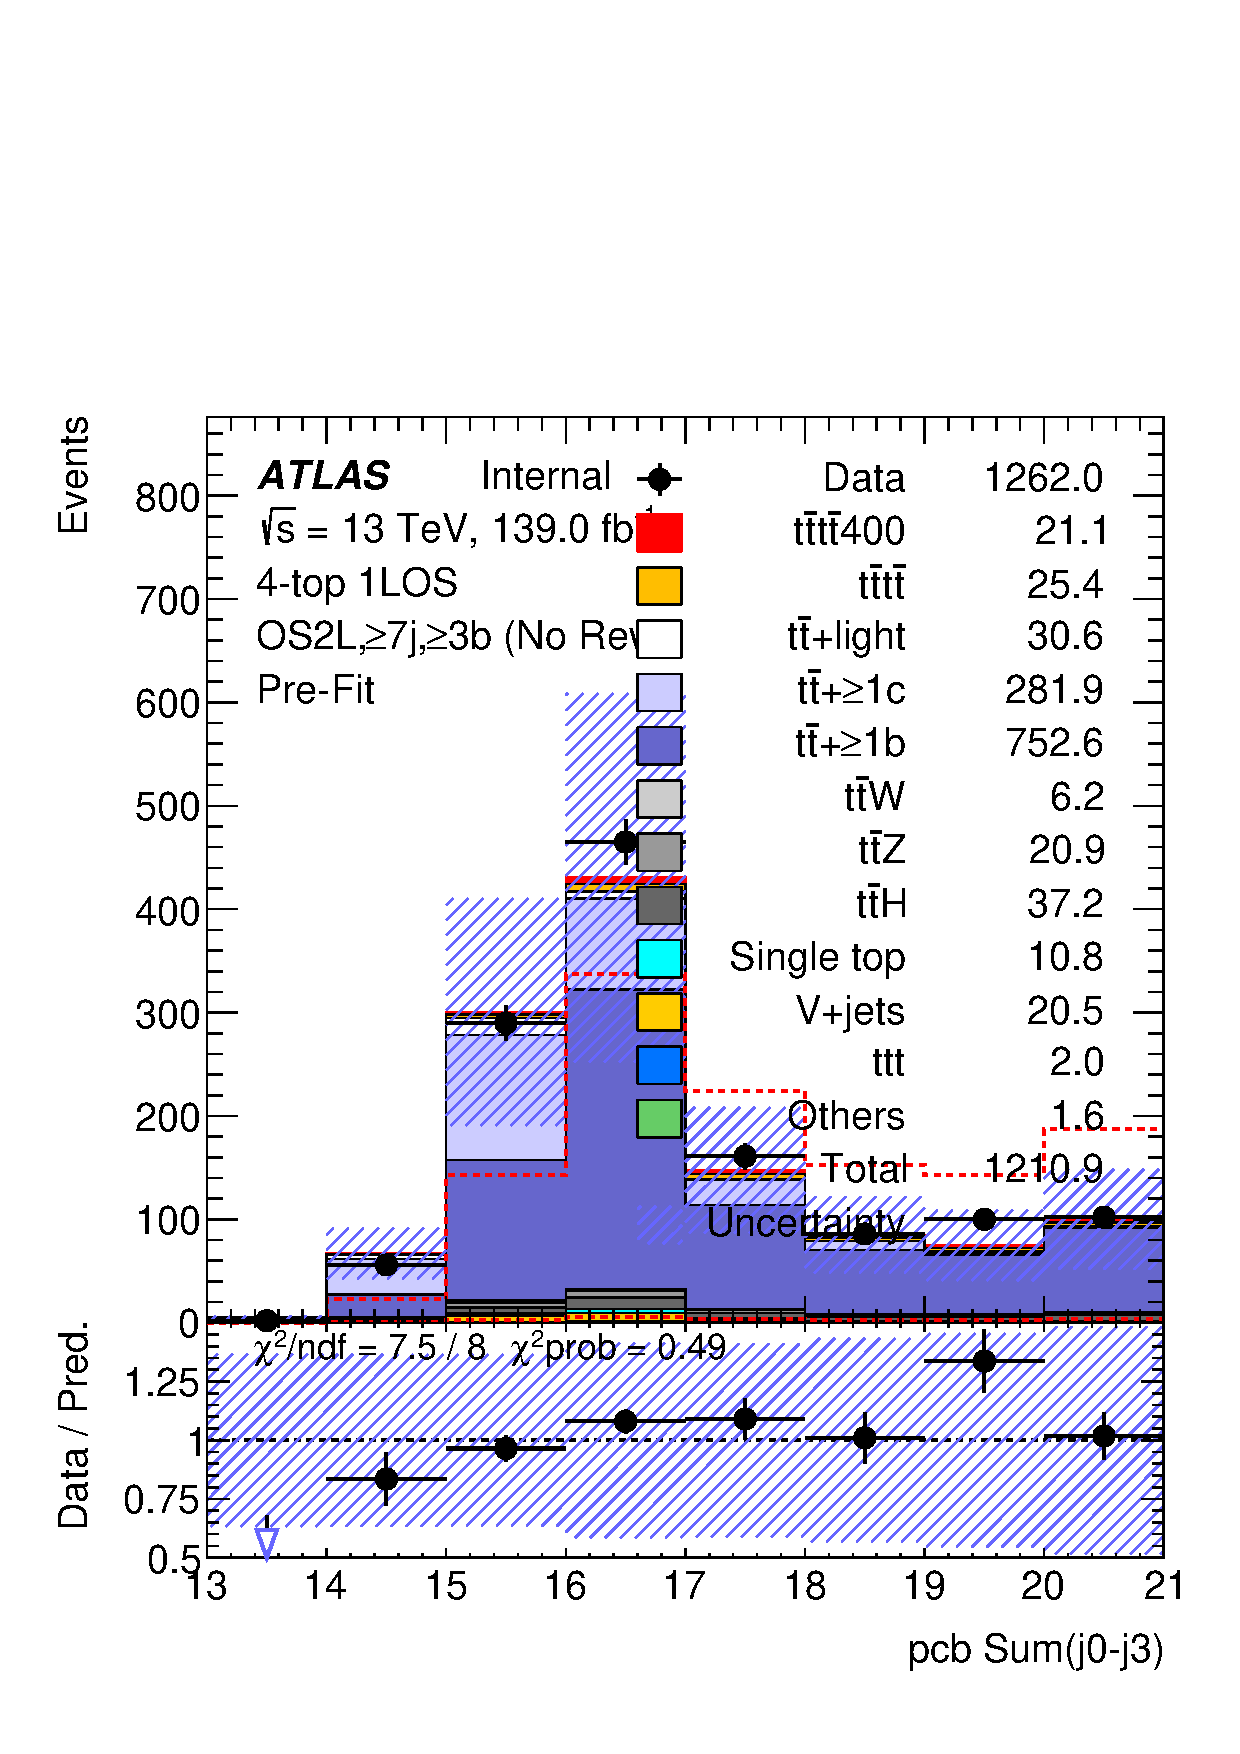
\includegraphics[width=0.3\textwidth]{figures/NNPlots/MVATrainRegion/NoRew/os2l_ge7jge3b_pcb.pdf}
    
\includegraphics[width=0.3\textwidth]{figures/NNPlots/MVATrainRegion/Rew/os2l_ge7jge3b_pcb.pdf}
    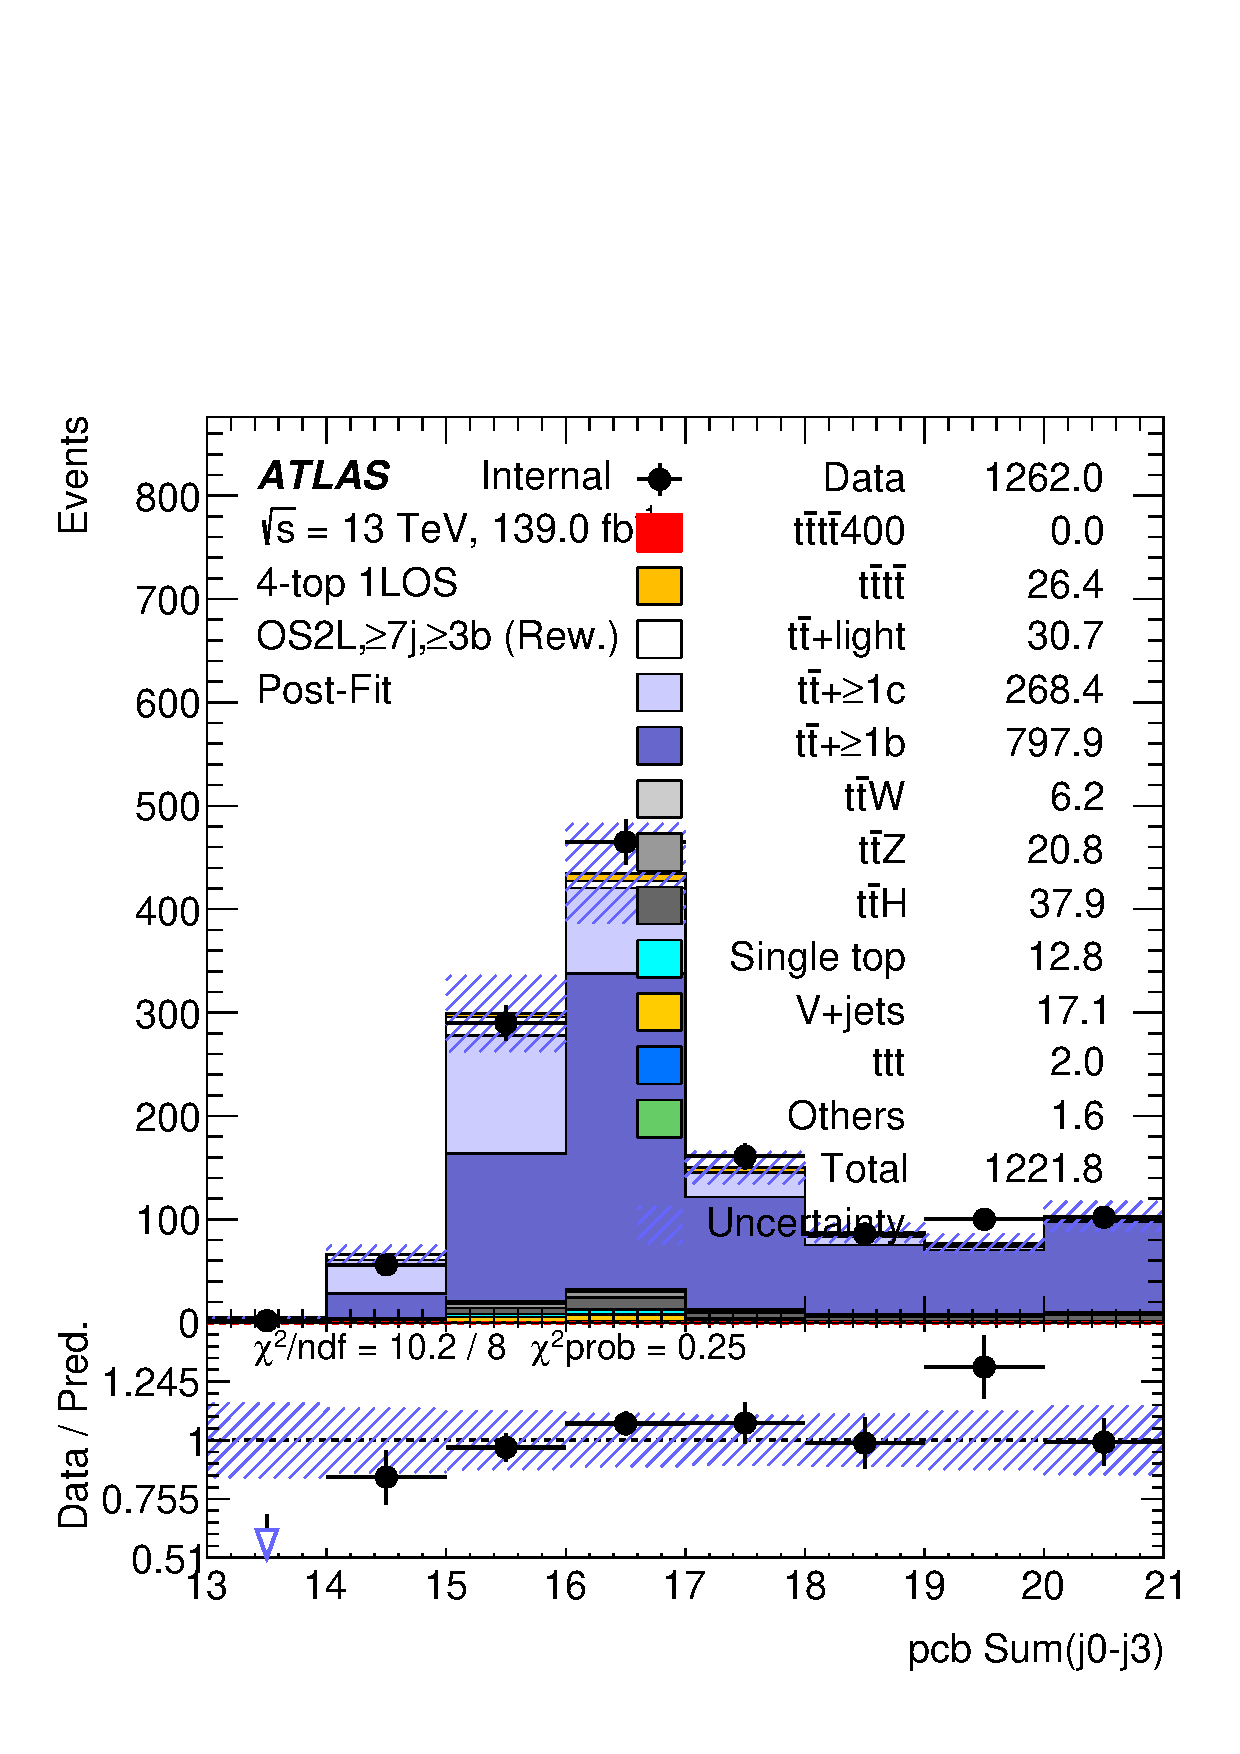
\includegraphics[width=0.3\textwidth]{figures/NNPlots/MVATrainRegion/Rew/os2l_ge7jge3b_pcb_postFit.pdf}
    \caption{pcb Sum}
    \end{center}
    \end{subfigure}

    \begin{subfigure}[t]{1\textwidth}
    \begin{center}
    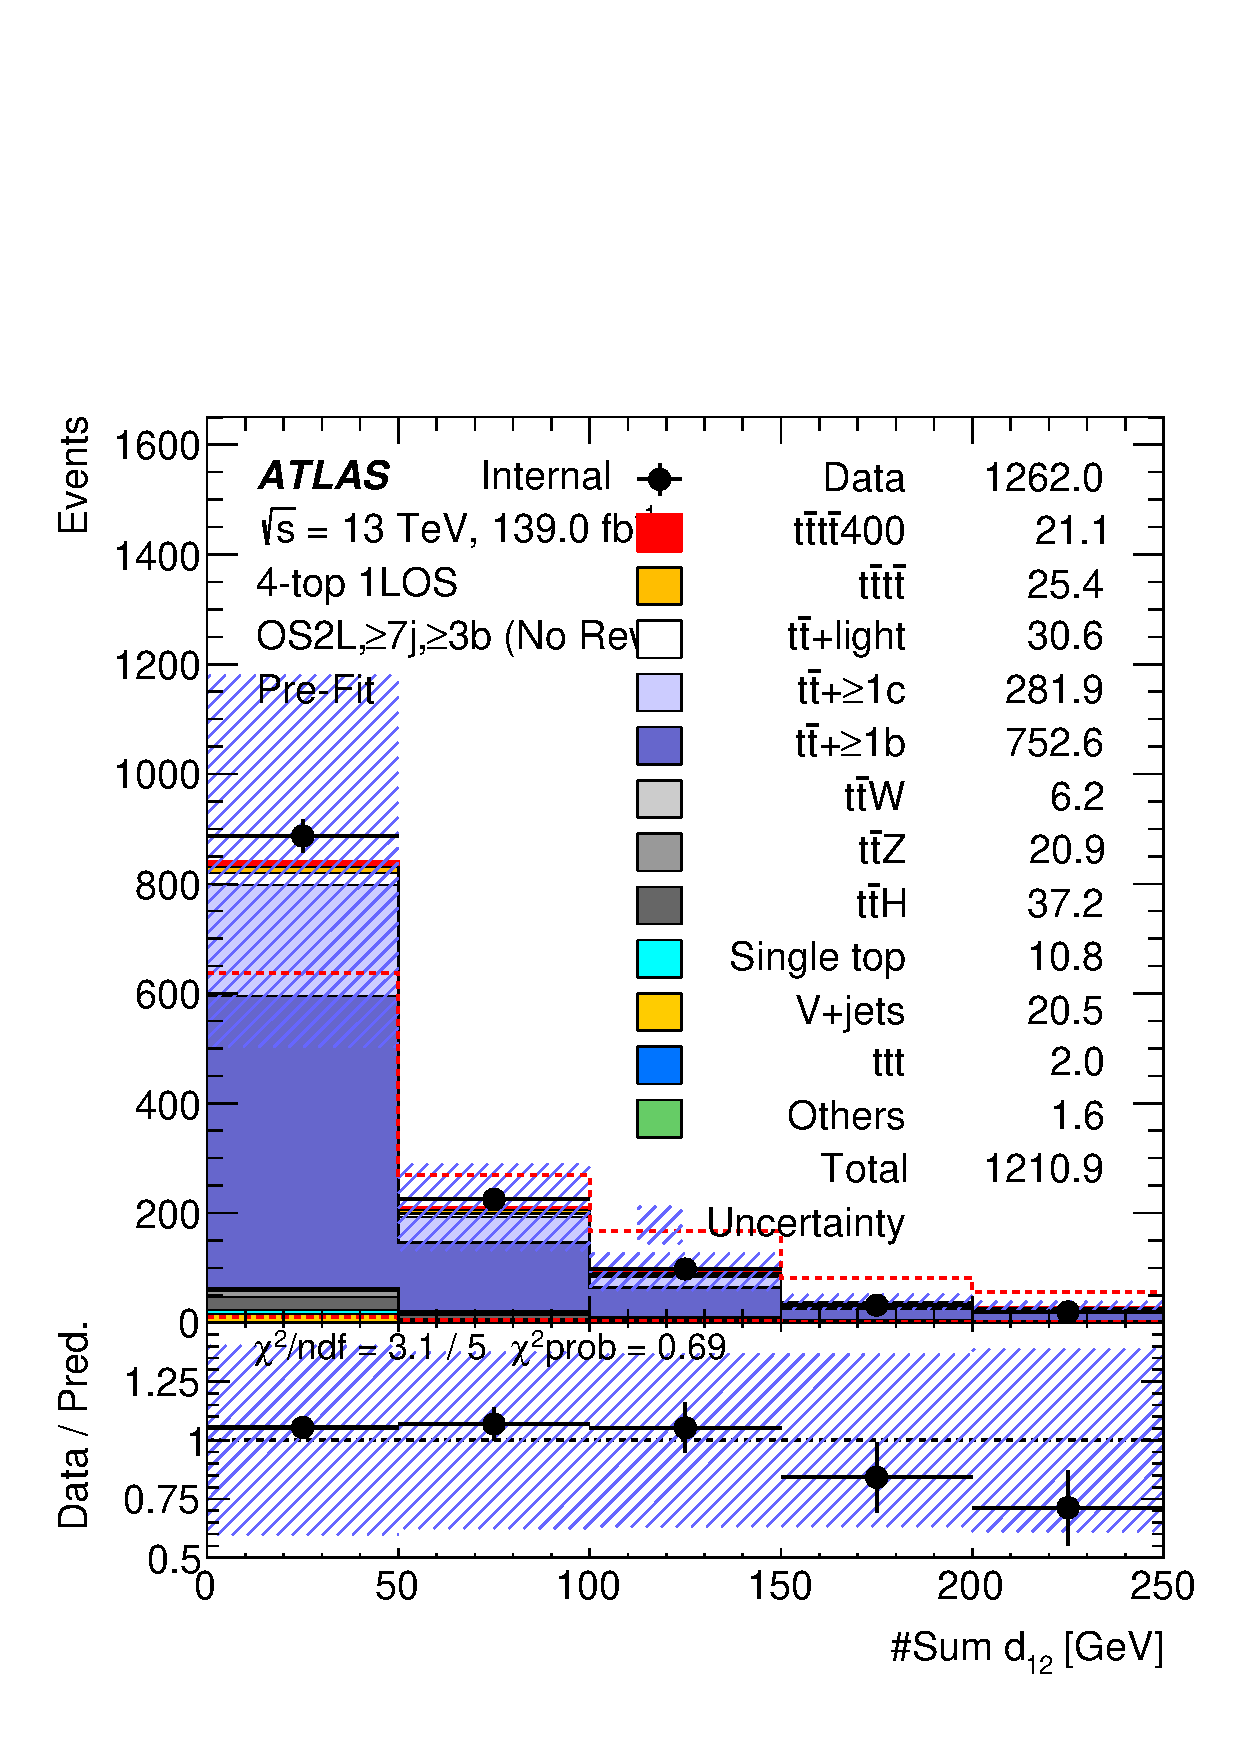
\includegraphics[width=0.3\textwidth]{figures/NNPlots/MVATrainRegion/NoRew/os2l_ge7jge3b_sum_d12.pdf}
    
\includegraphics[width=0.3\textwidth]{figures/NNPlots/MVATrainRegion/Rew/os2l_ge7jge3b_sum_d12.pdf}
    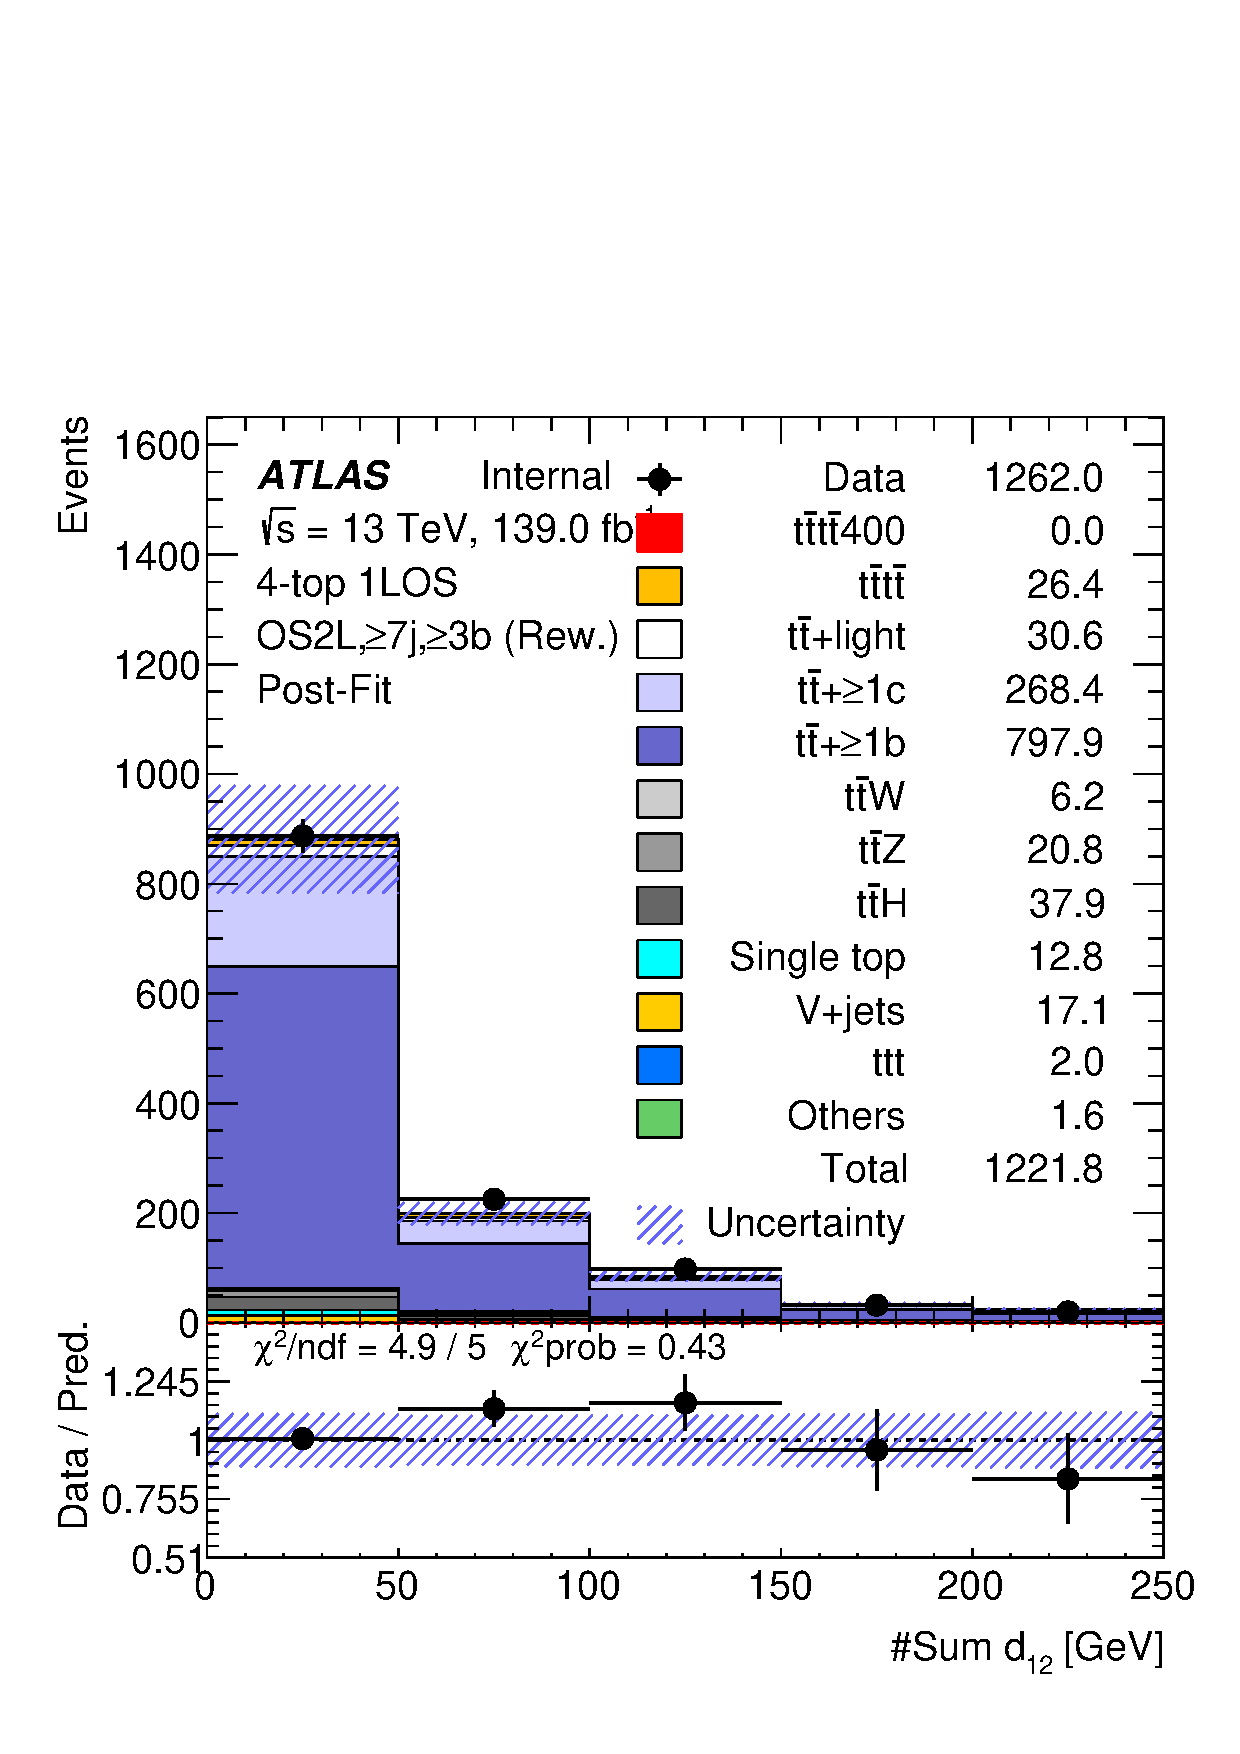
\includegraphics[width=0.3\textwidth]{figures/NNPlots/MVATrainRegion/Rew/os2l_ge7jge3b_sum_d12_postFit.pdf}
    \caption{$\sum d_{12}$}
    \end{center}
    \end{subfigure}

    \begin{subfigure}[t]{1\textwidth}
    \begin{center}
    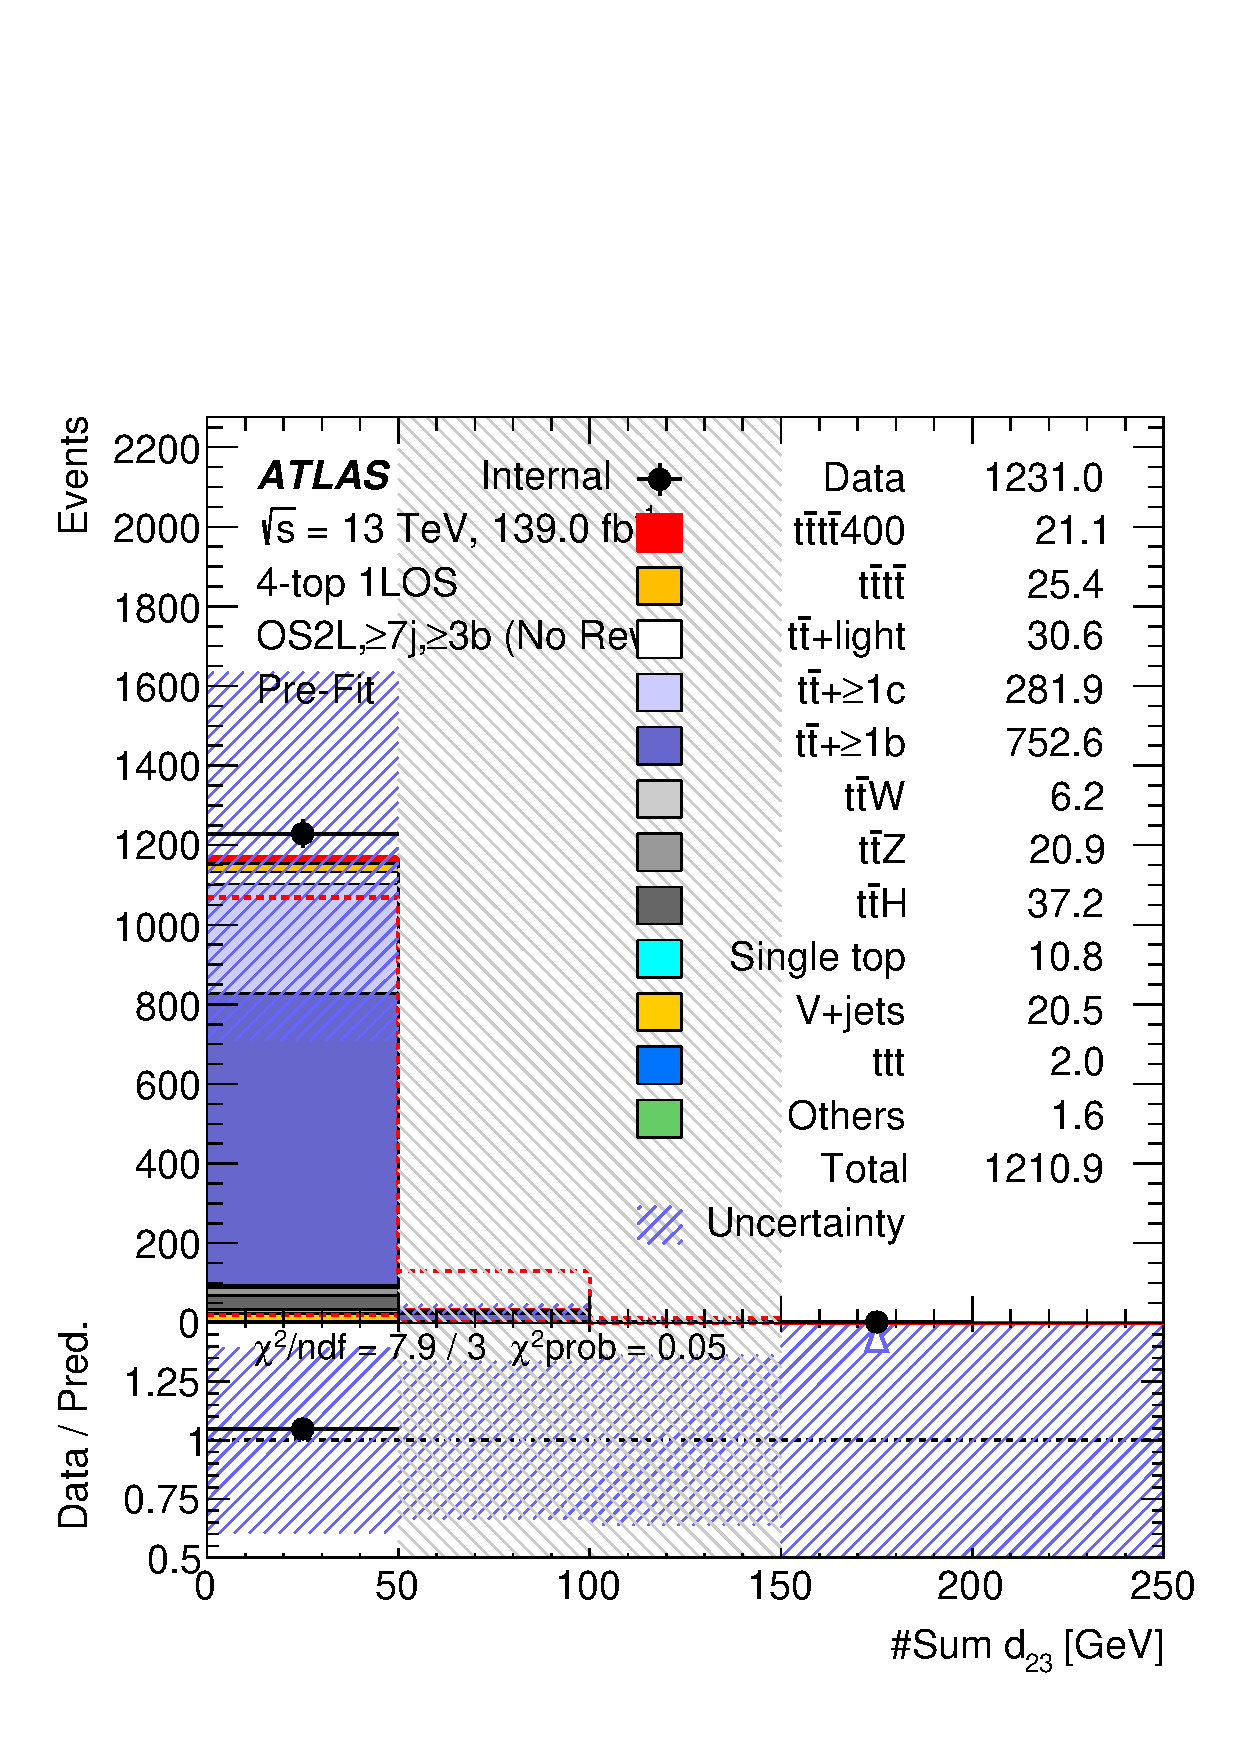
\includegraphics[width=0.3\textwidth]{figures/NNPlots/MVATrainRegion/NoRew/os2l_ge7jge3b_sum_d23.pdf}
    
\includegraphics[width=0.3\textwidth]{figures/NNPlots/MVATrainRegion/Rew/os2l_ge7jge3b_sum_d23.pdf}
    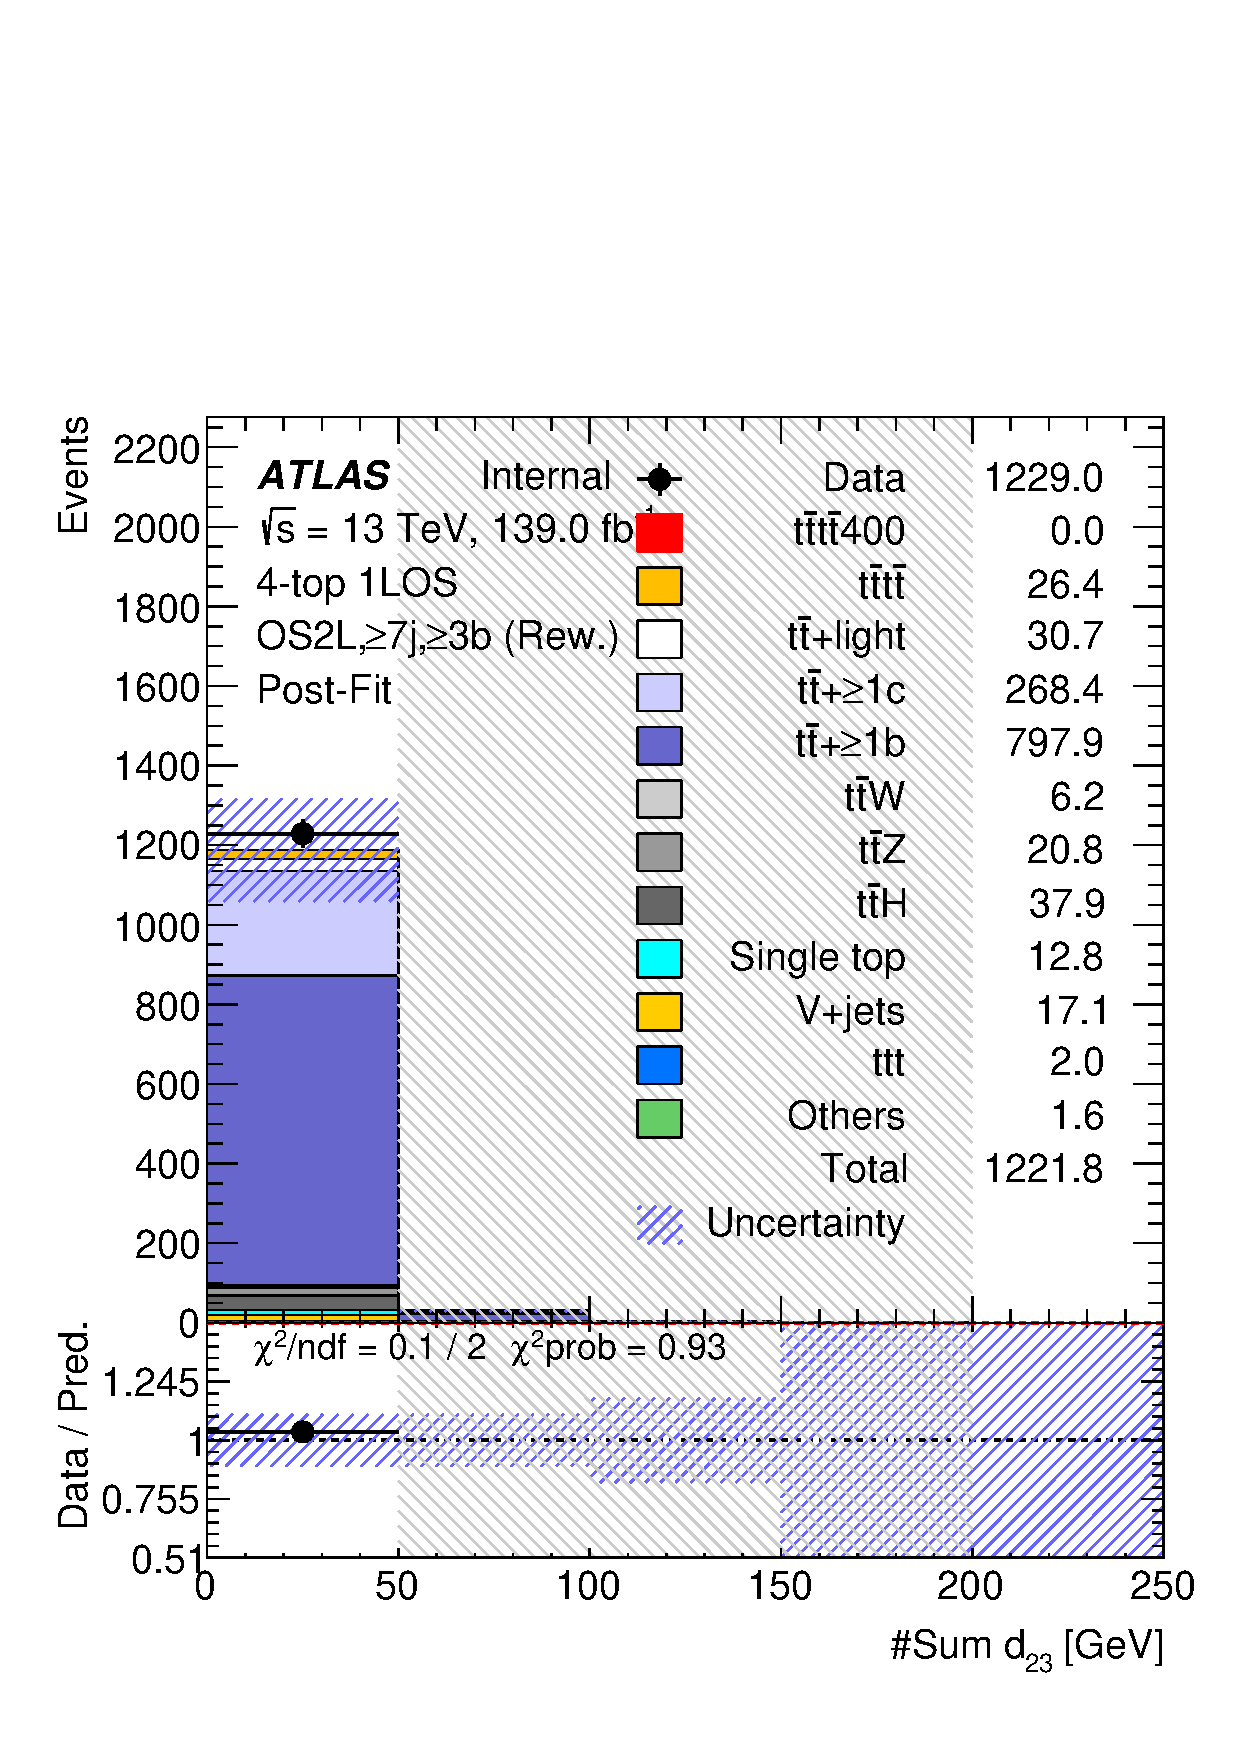
\includegraphics[width=0.3\textwidth]{figures/NNPlots/MVATrainRegion/Rew/os2l_ge7jge3b_sum_d23_postFit.pdf}
    \caption{$\sum d_{23}$}
    \end{center}
    \end{subfigure}
    \caption{\label{fig:NNPlots_MVATrainReg_10} The comparison between variables pre-fit distribution before (left) and after (middle) the NN-reweighting  in 1L MVA training regions ($\geq 7j,\geq 3b$). The post-fit distribution after the NN-reweighting is shown on the left. Blinded regions are excluded.}
\end{figure}

\begin{figure}[htbp!]
    \begin{subfigure}[t]{1\textwidth}
    \begin{center}
    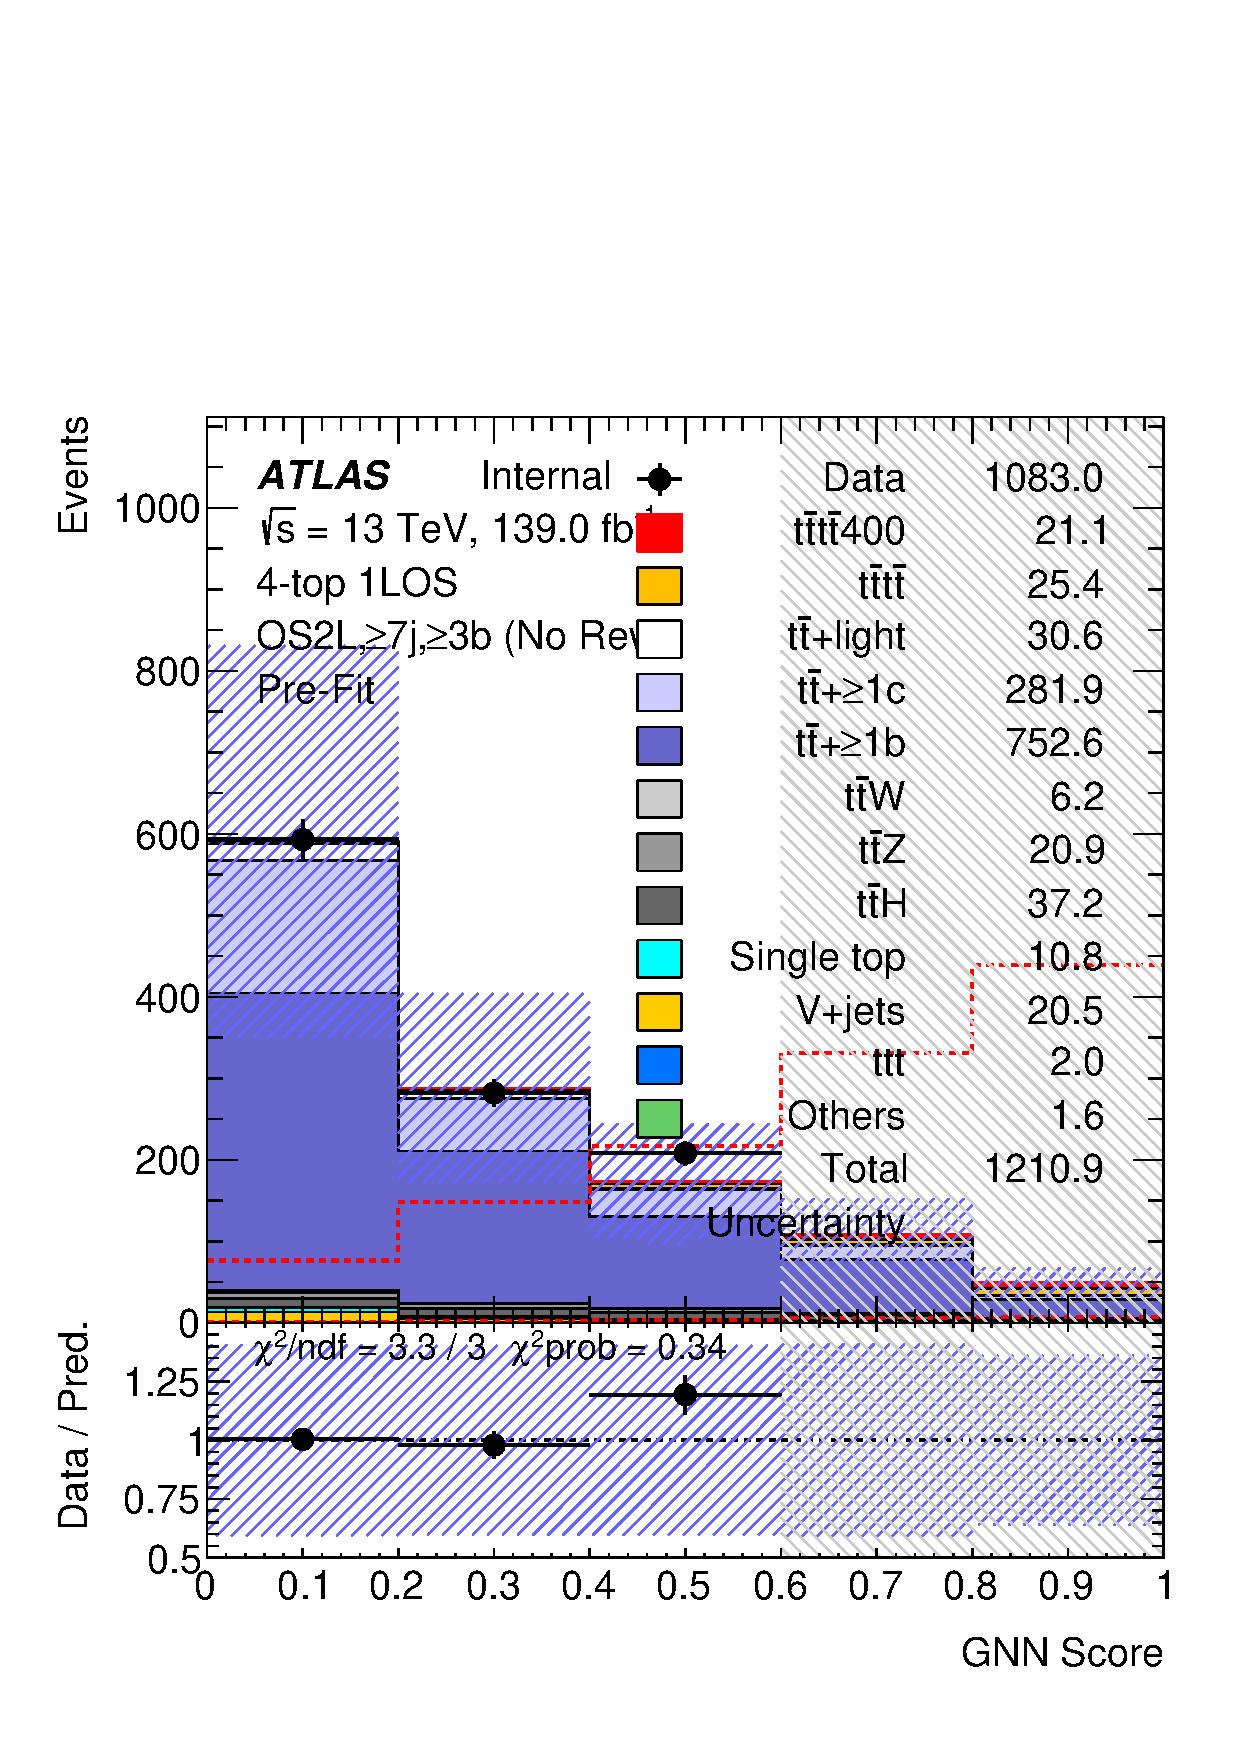
\includegraphics[width=0.3\textwidth]{figures/NNPlots/MVATrainRegion/NoRew/os2l_ge7jge3b_GNN.pdf}
    
\includegraphics[width=0.3\textwidth]{figures/NNPlots/MVATrainRegion/Rew/os2l_ge7jge3b_GNN.pdf}
    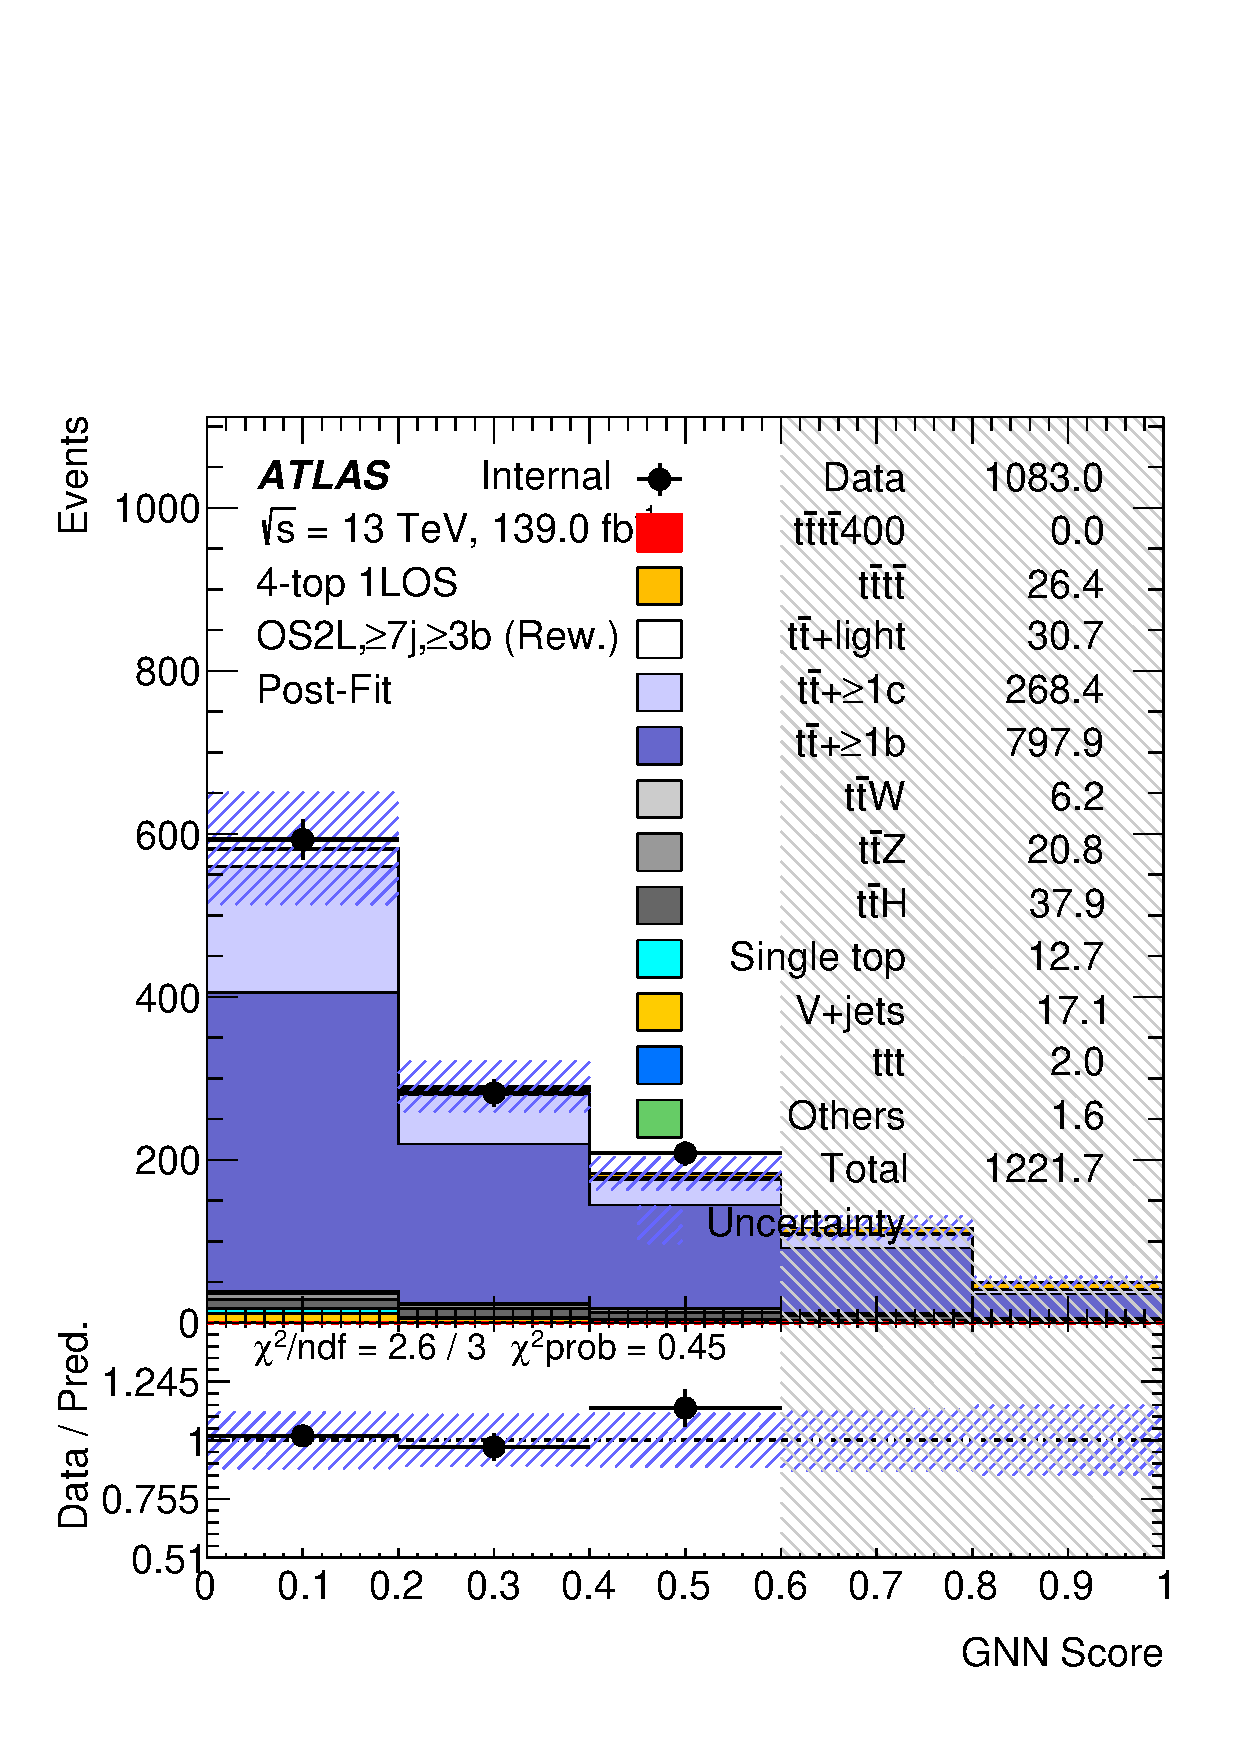
\includegraphics[width=0.3\textwidth]{figures/NNPlots/MVATrainRegion/Rew/os2l_ge7jge3b_GNN_postFit.pdf}
    \caption{GNN Score}
    \end{center}
    \end{subfigure}
    \caption{\label{fig:NNPlots_MVATrainReg_10} The comparison between variables pre-fit distribution before (left) and after (middle) the NN-reweighting  in 1L MVA training regions ($\geq 7j,\geq 3b$). The post-fit distribution after the NN-reweighting is shown on the left. Blinded regions are excluded.}
\end{figure}

\clearpage

%%% NN Training Regions %%%
\subsection{NN Training Regions (ge7j(ge5j)2b)}
\begin{figure}[htbp!]
    \begin{subfigure}[t]{1\textwidth}
    \begin{center}
    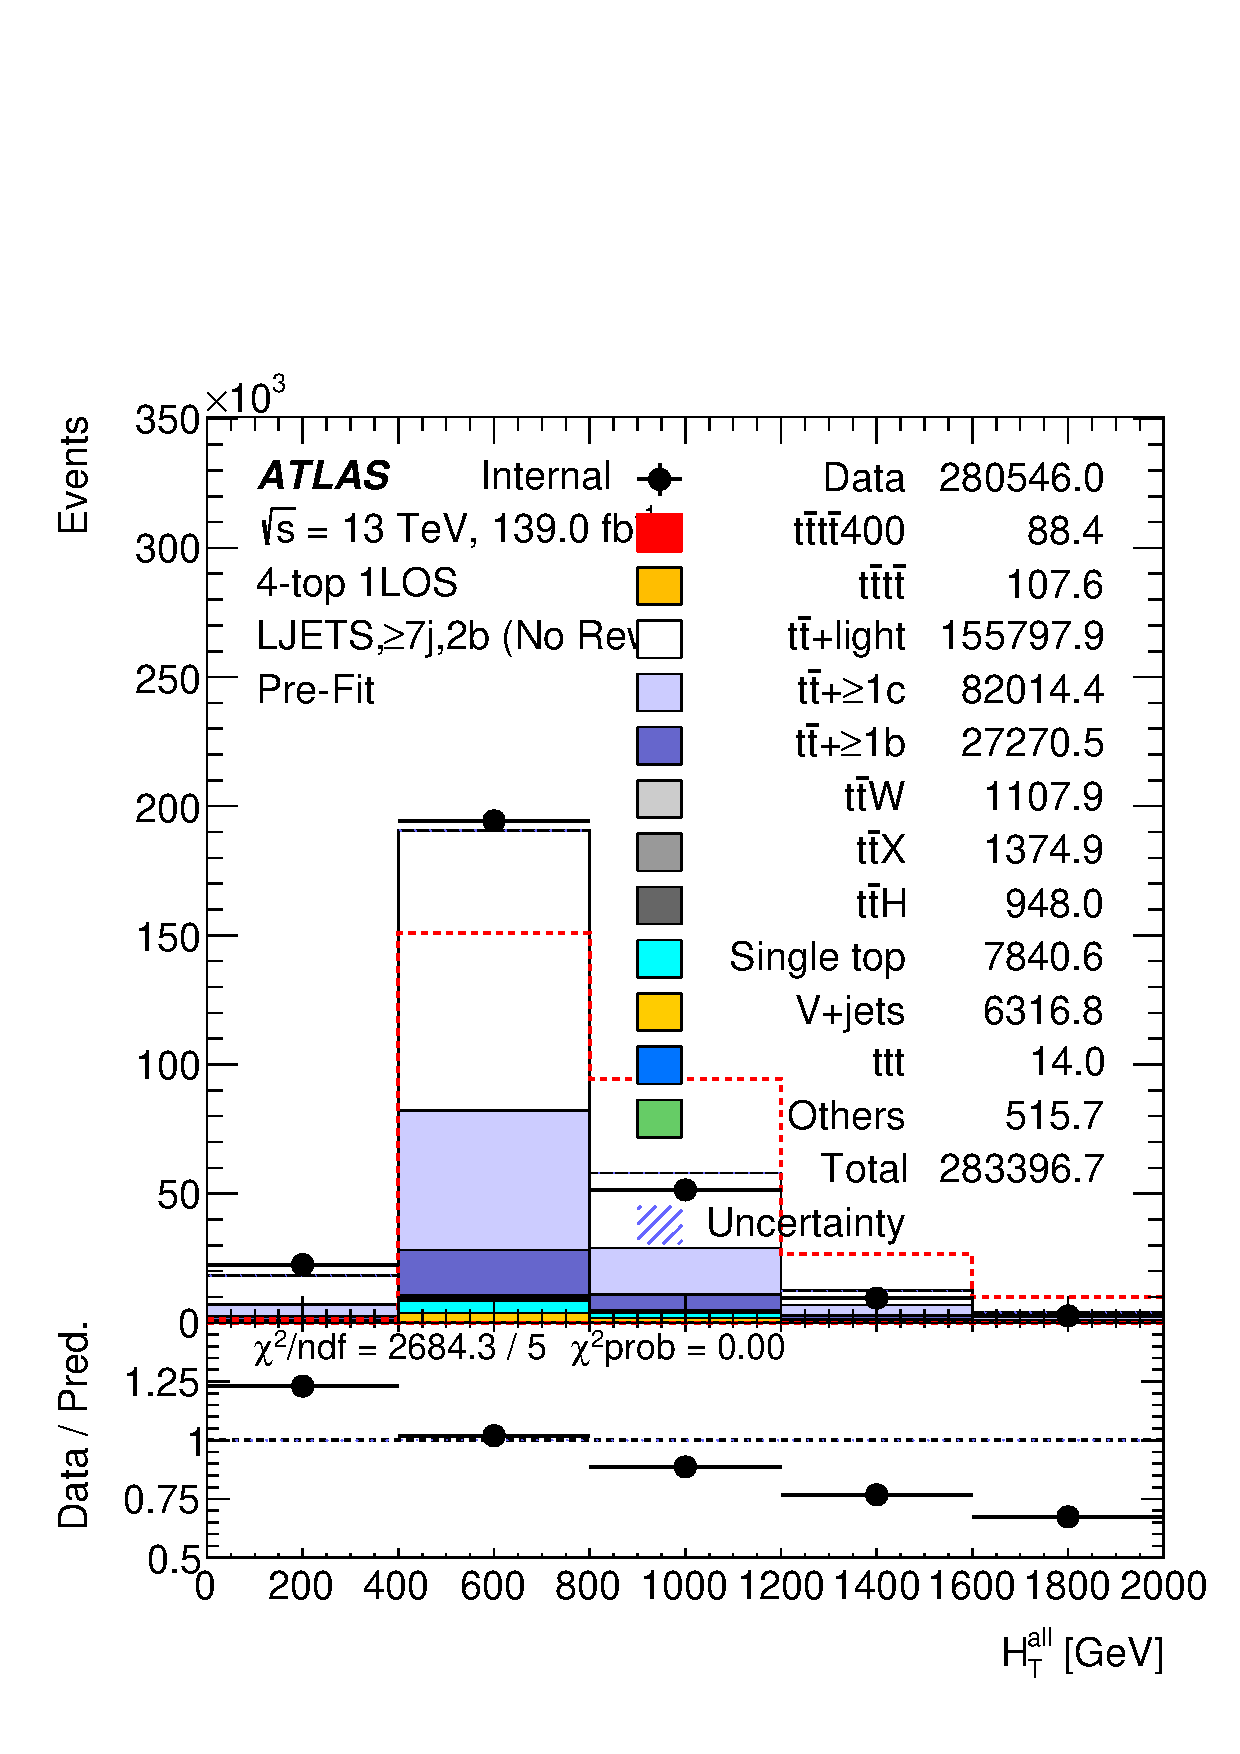
\includegraphics[width=0.4\textwidth]{figures/NNPlots/NNTrainRegion/NoRew/ljets_ge7j2b_HT.pdf}
    
\includegraphics[width=0.4\textwidth]{figures/NNPlots/NNTrainRegion/Rew/ljets_ge7j2b_HT.pdf}
    \caption{$H_{T}$}
    \end{center}
    \end{subfigure}

    \begin{subfigure}[t]{1\textwidth}
    \begin{center}
    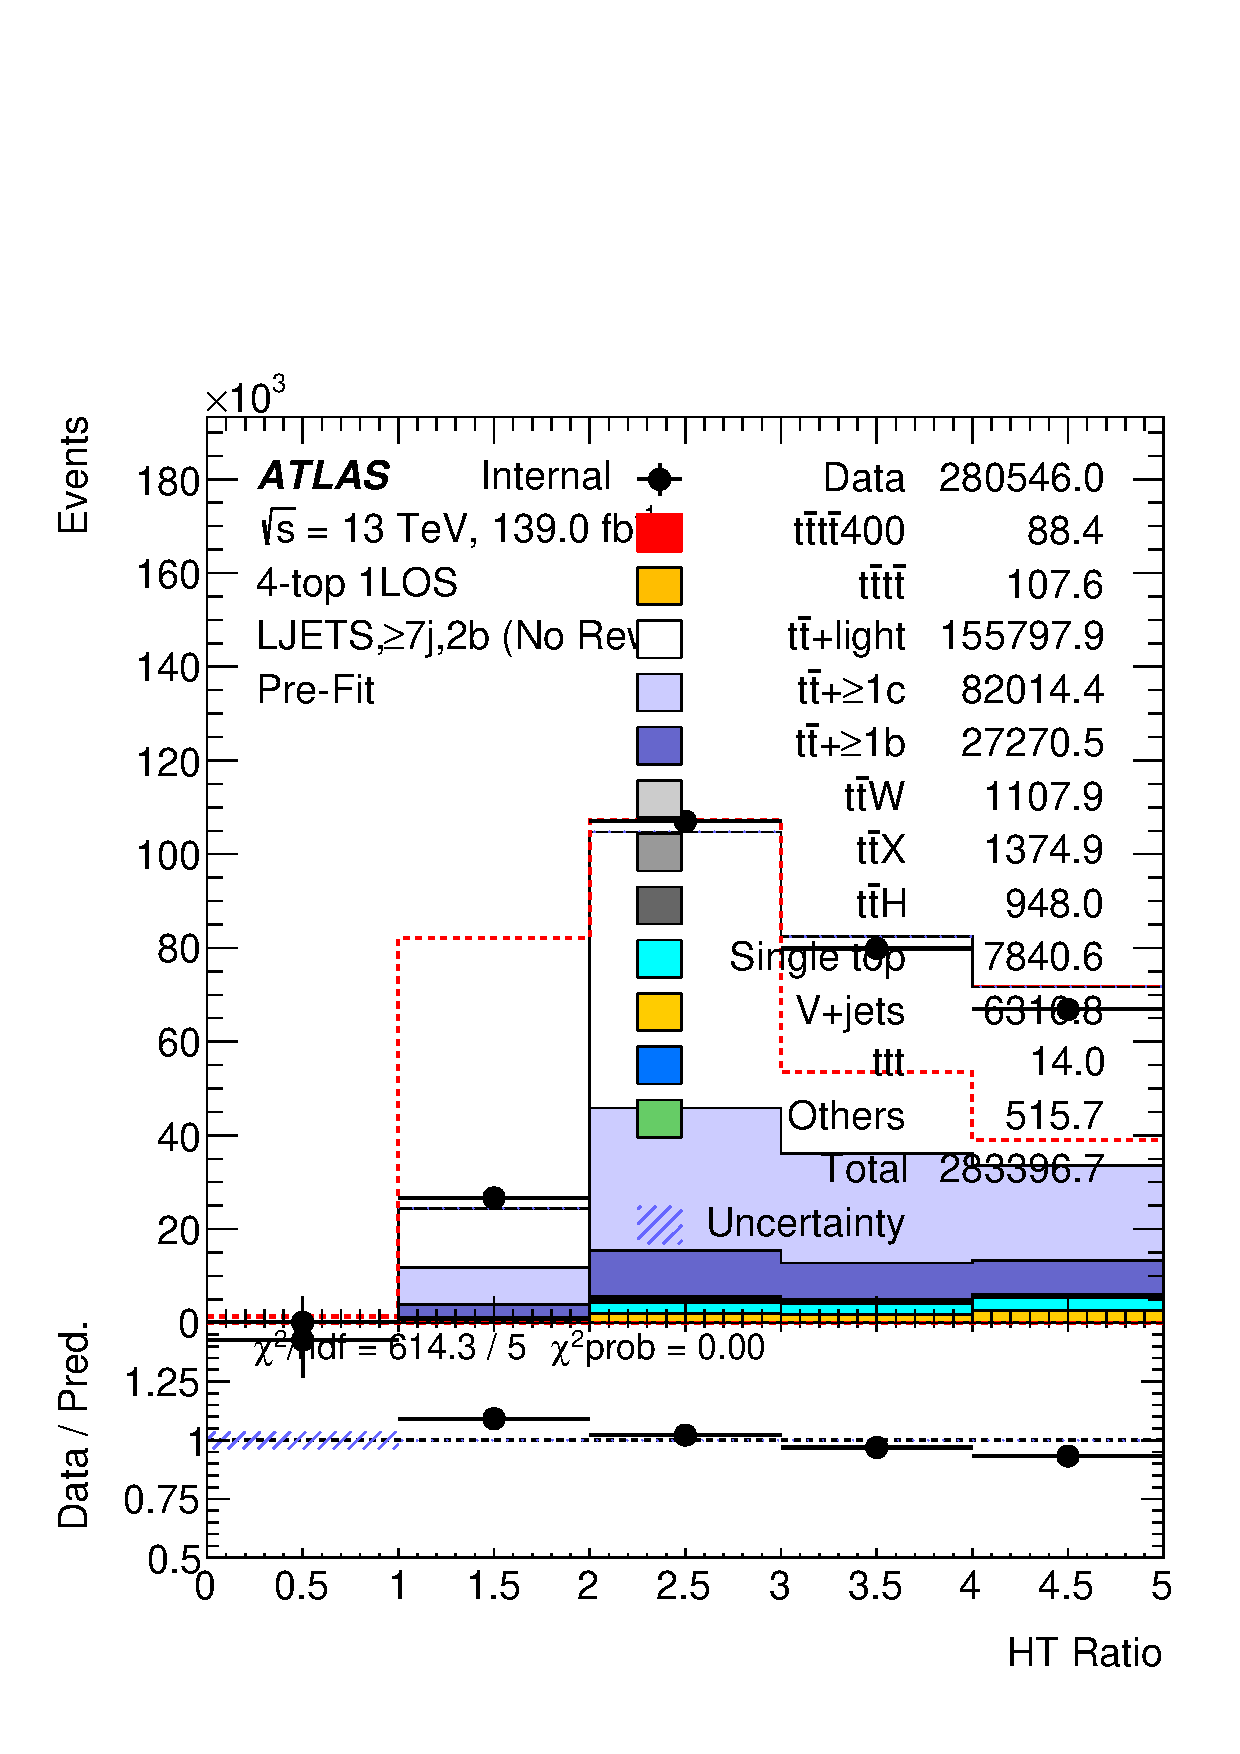
\includegraphics[width=0.4\textwidth]{figures/NNPlots/NNTrainRegion/NoRew/ljets_ge7j2b_HTRatio.pdf}
    
\includegraphics[width=0.4\textwidth]{figures/NNPlots/NNTrainRegion/Rew/ljets_ge7j2b_HTRatio.pdf}
    \caption{HTRatio}
    \end{center}
    \end{subfigure}

    \begin{subfigure}[t]{1\textwidth}
    \begin{center}
    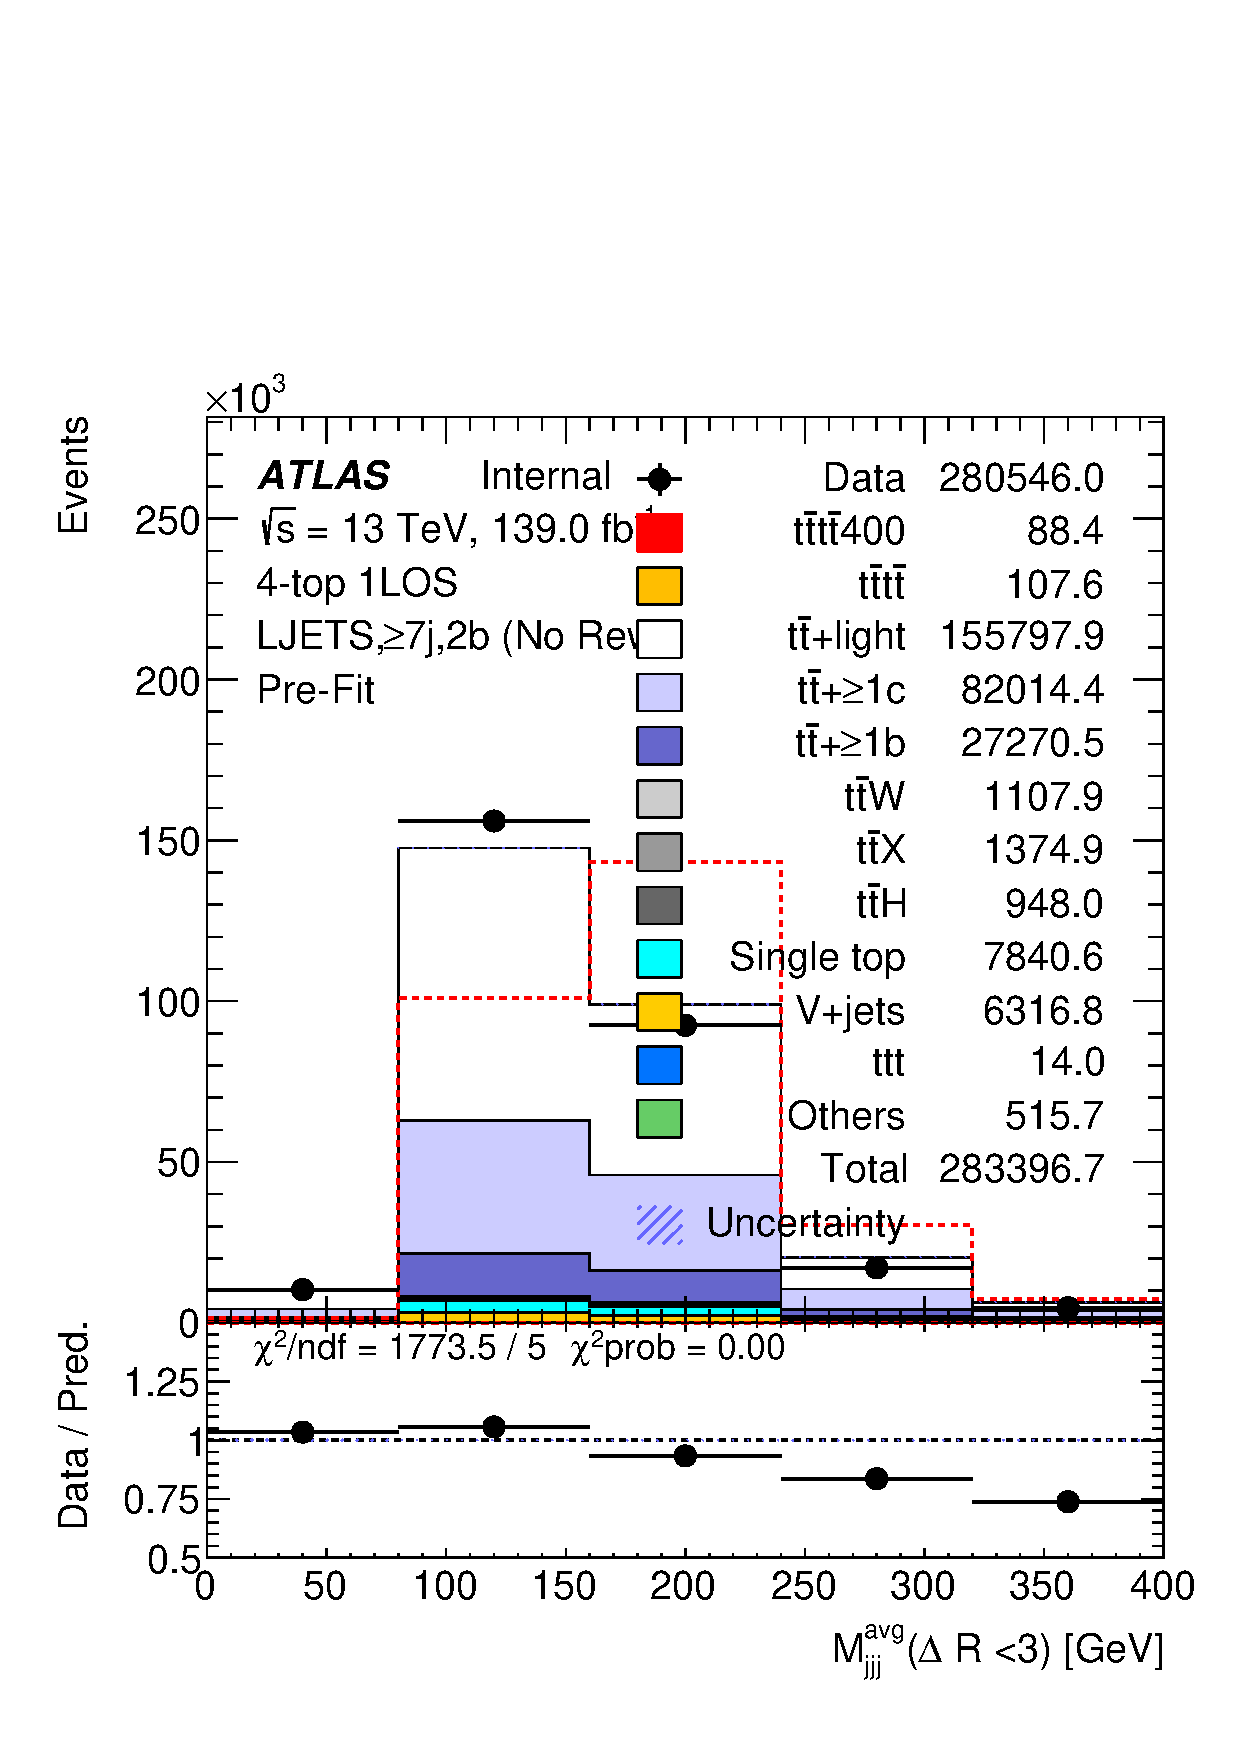
\includegraphics[width=0.4\textwidth]{figures/NNPlots/NNTrainRegion/NoRew/ljets_ge7j2b_Mjjj_AvgdRs3.pdf}
    
\includegraphics[width=0.4\textwidth]{figures/NNPlots/NNTrainRegion/Rew/ljets_ge7j2b_Mjjj_AvgdRs3.pdf}
    \caption{$M^{avg}_{jjj}(\Delta R <3)$}
    \end{center}
    \end{subfigure}
    \caption{\label{fig:NNPlots_NNTrainReg_1} The comparison between variables distribution before (left) and after (right) the NN-reweighting in 1L NN training regions ($\geq 7j,=2b$). Blinded regions are excluded.}  
\end{figure}

\begin{figure}[htbp!]
    \begin{subfigure}[t]{1\textwidth}
    \begin{center}
    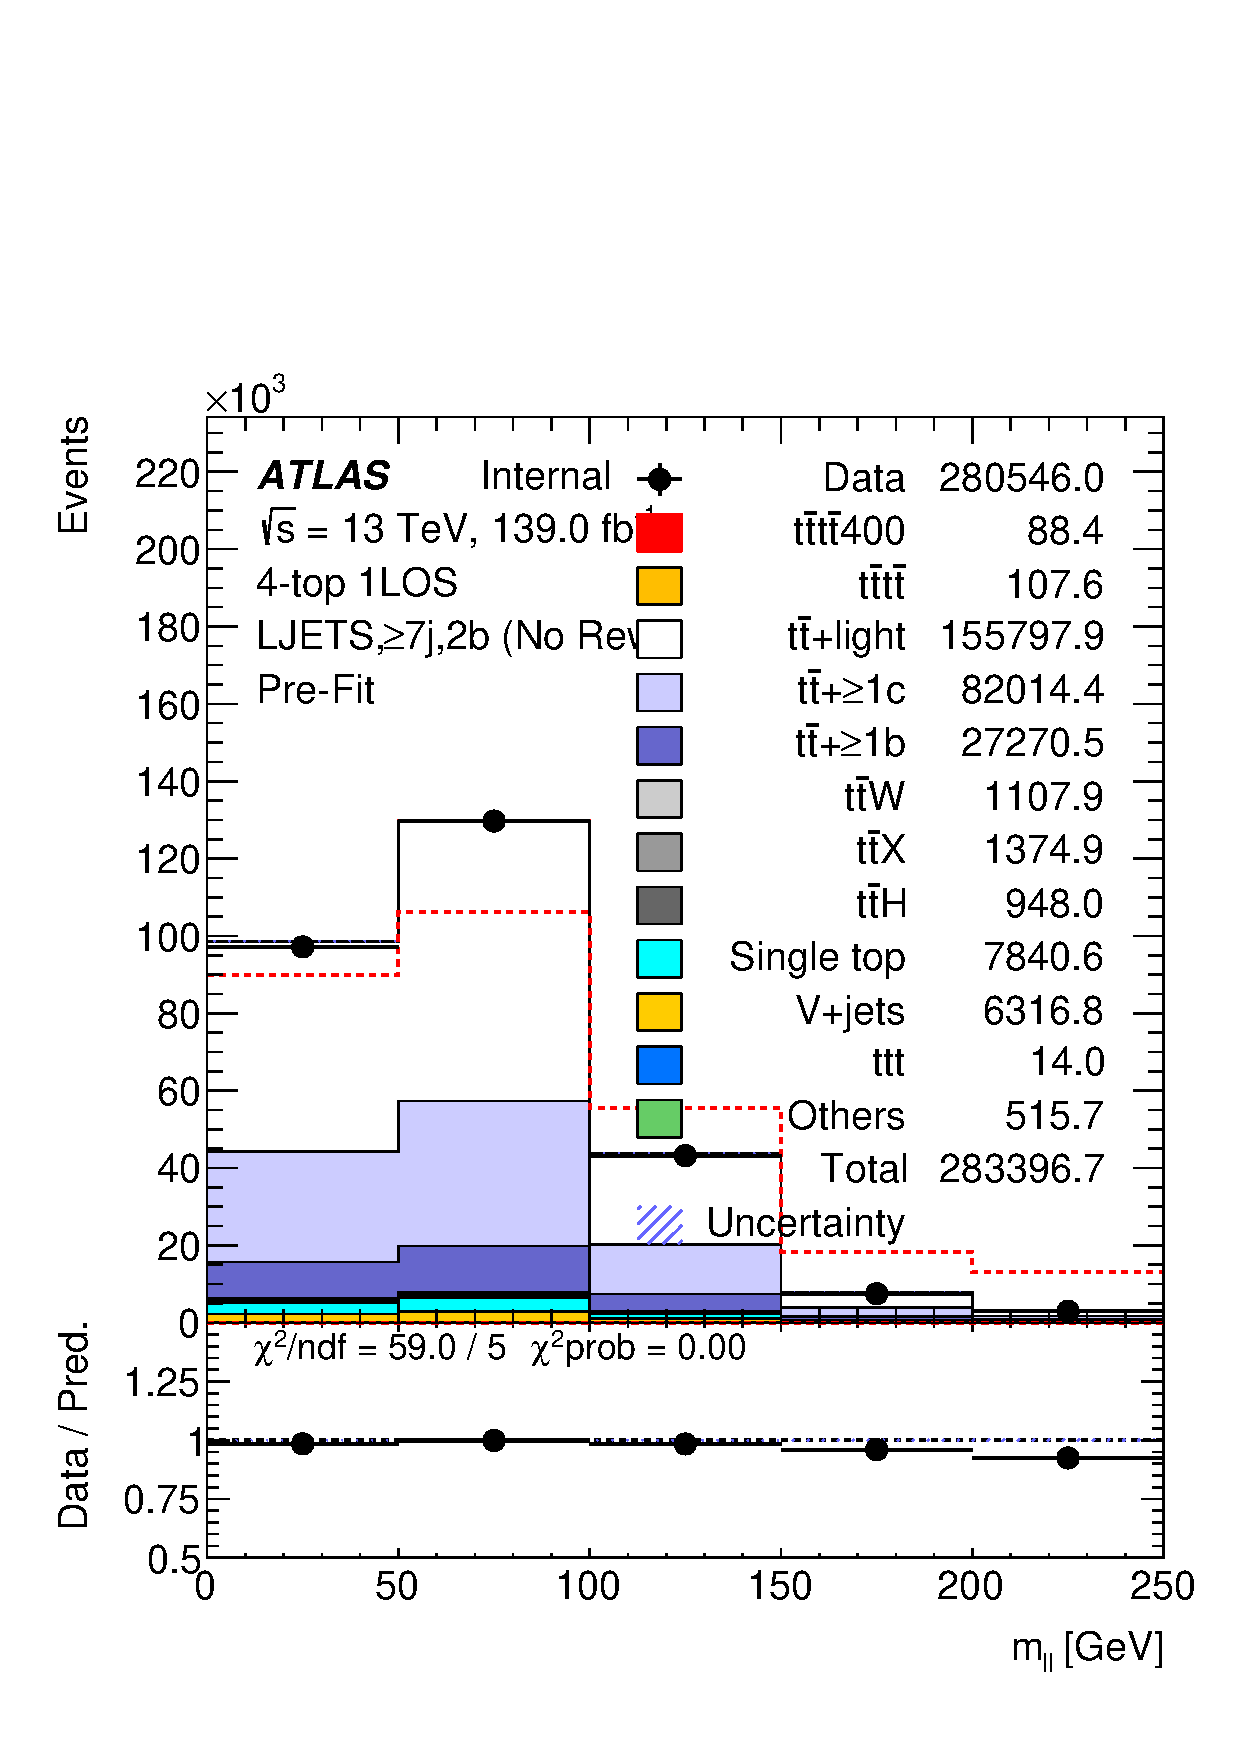
\includegraphics[width=0.4\textwidth]{figures/NNPlots/NNTrainRegion/NoRew/ljets_ge7j2b_mtw.pdf}
    
\includegraphics[width=0.4\textwidth]{figures/NNPlots/NNTrainRegion/Rew/ljets_ge7j2b_mtw.pdf}
    \caption{mtw}
    \end{center}
    \end{subfigure}

    \begin{subfigure}[t]{1\textwidth}
    \begin{center}
    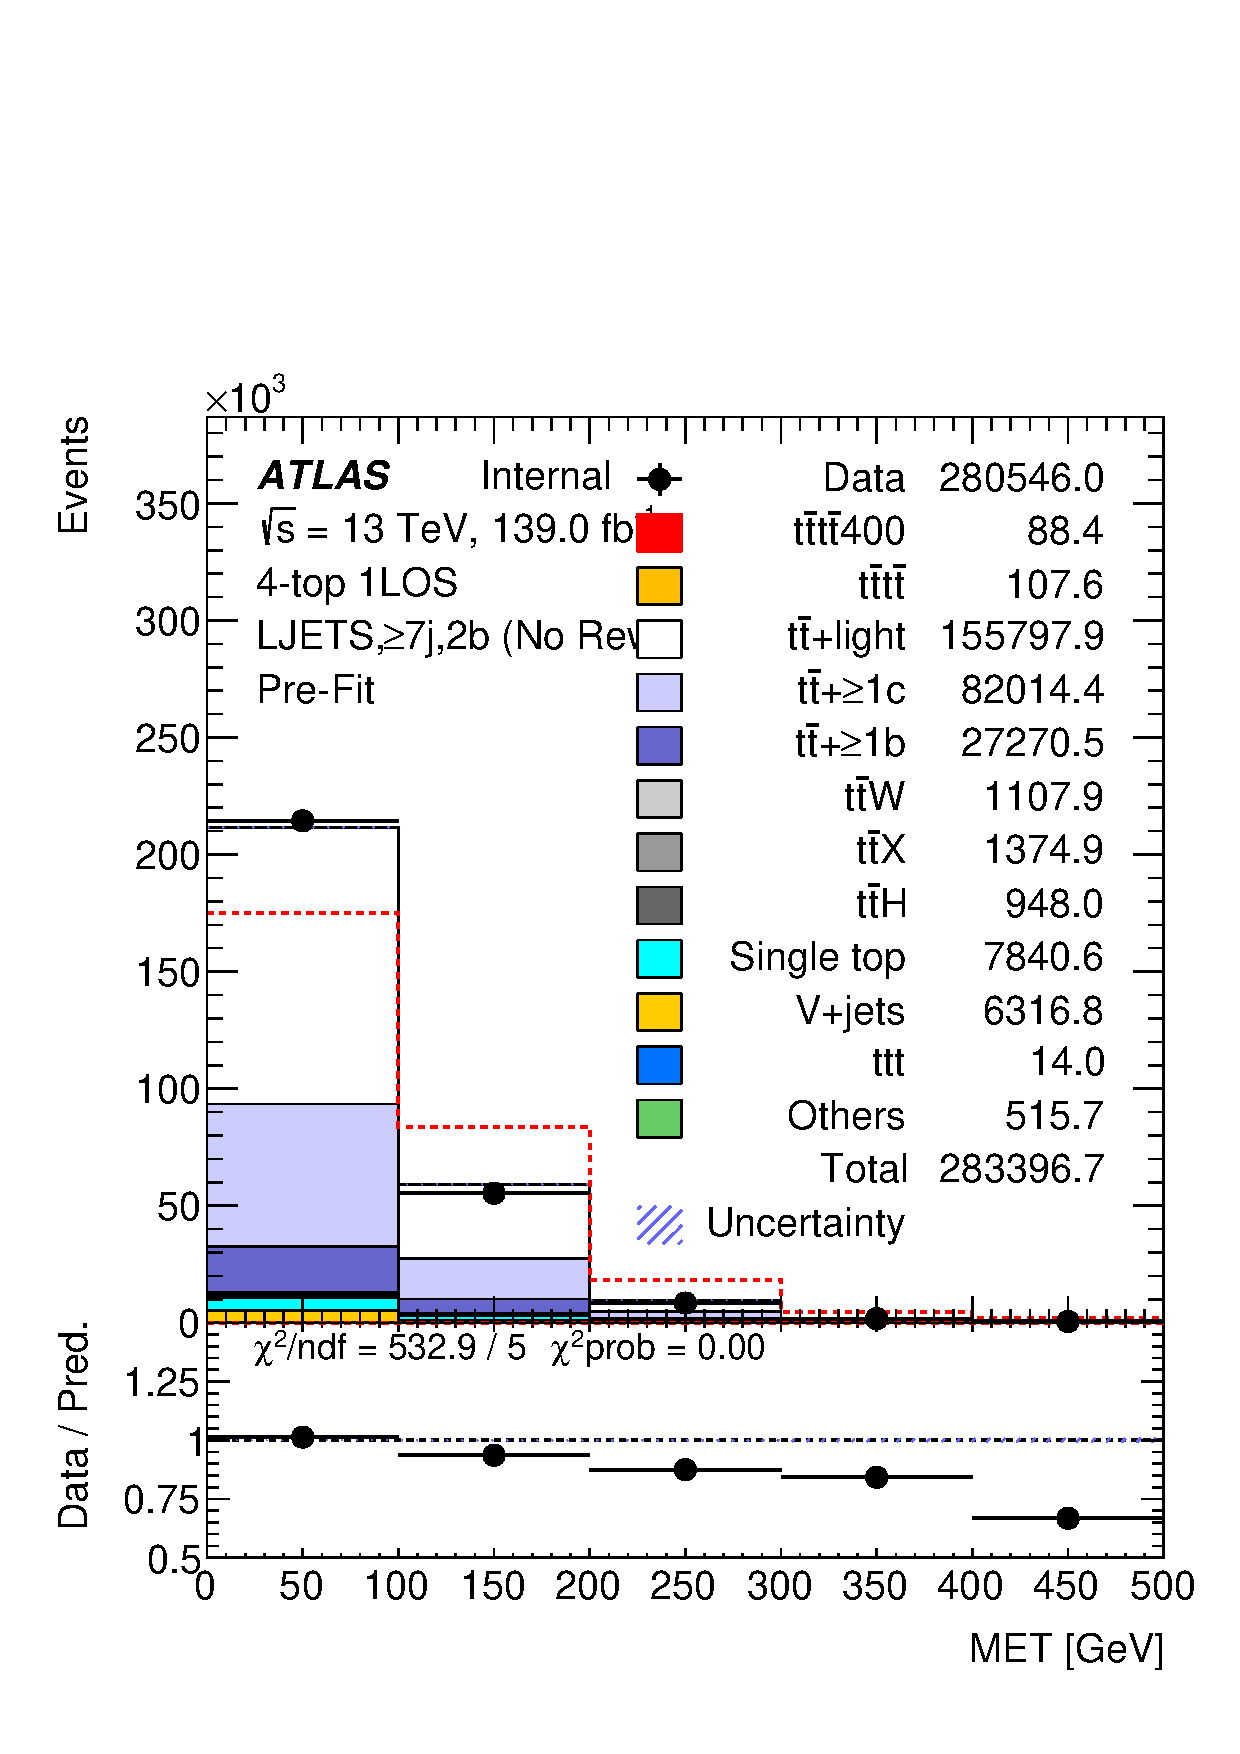
\includegraphics[width=0.4\textwidth]{figures/NNPlots/NNTrainRegion/NoRew/ljets_ge7j2b_met.pdf}
    
\includegraphics[width=0.4\textwidth]{figures/NNPlots/NNTrainRegion/Rew/ljets_ge7j2b_met.pdf}
    \caption{MET}
    \end{center}
    \end{subfigure}

    \begin{subfigure}[t]{1\textwidth}
    \begin{center}
    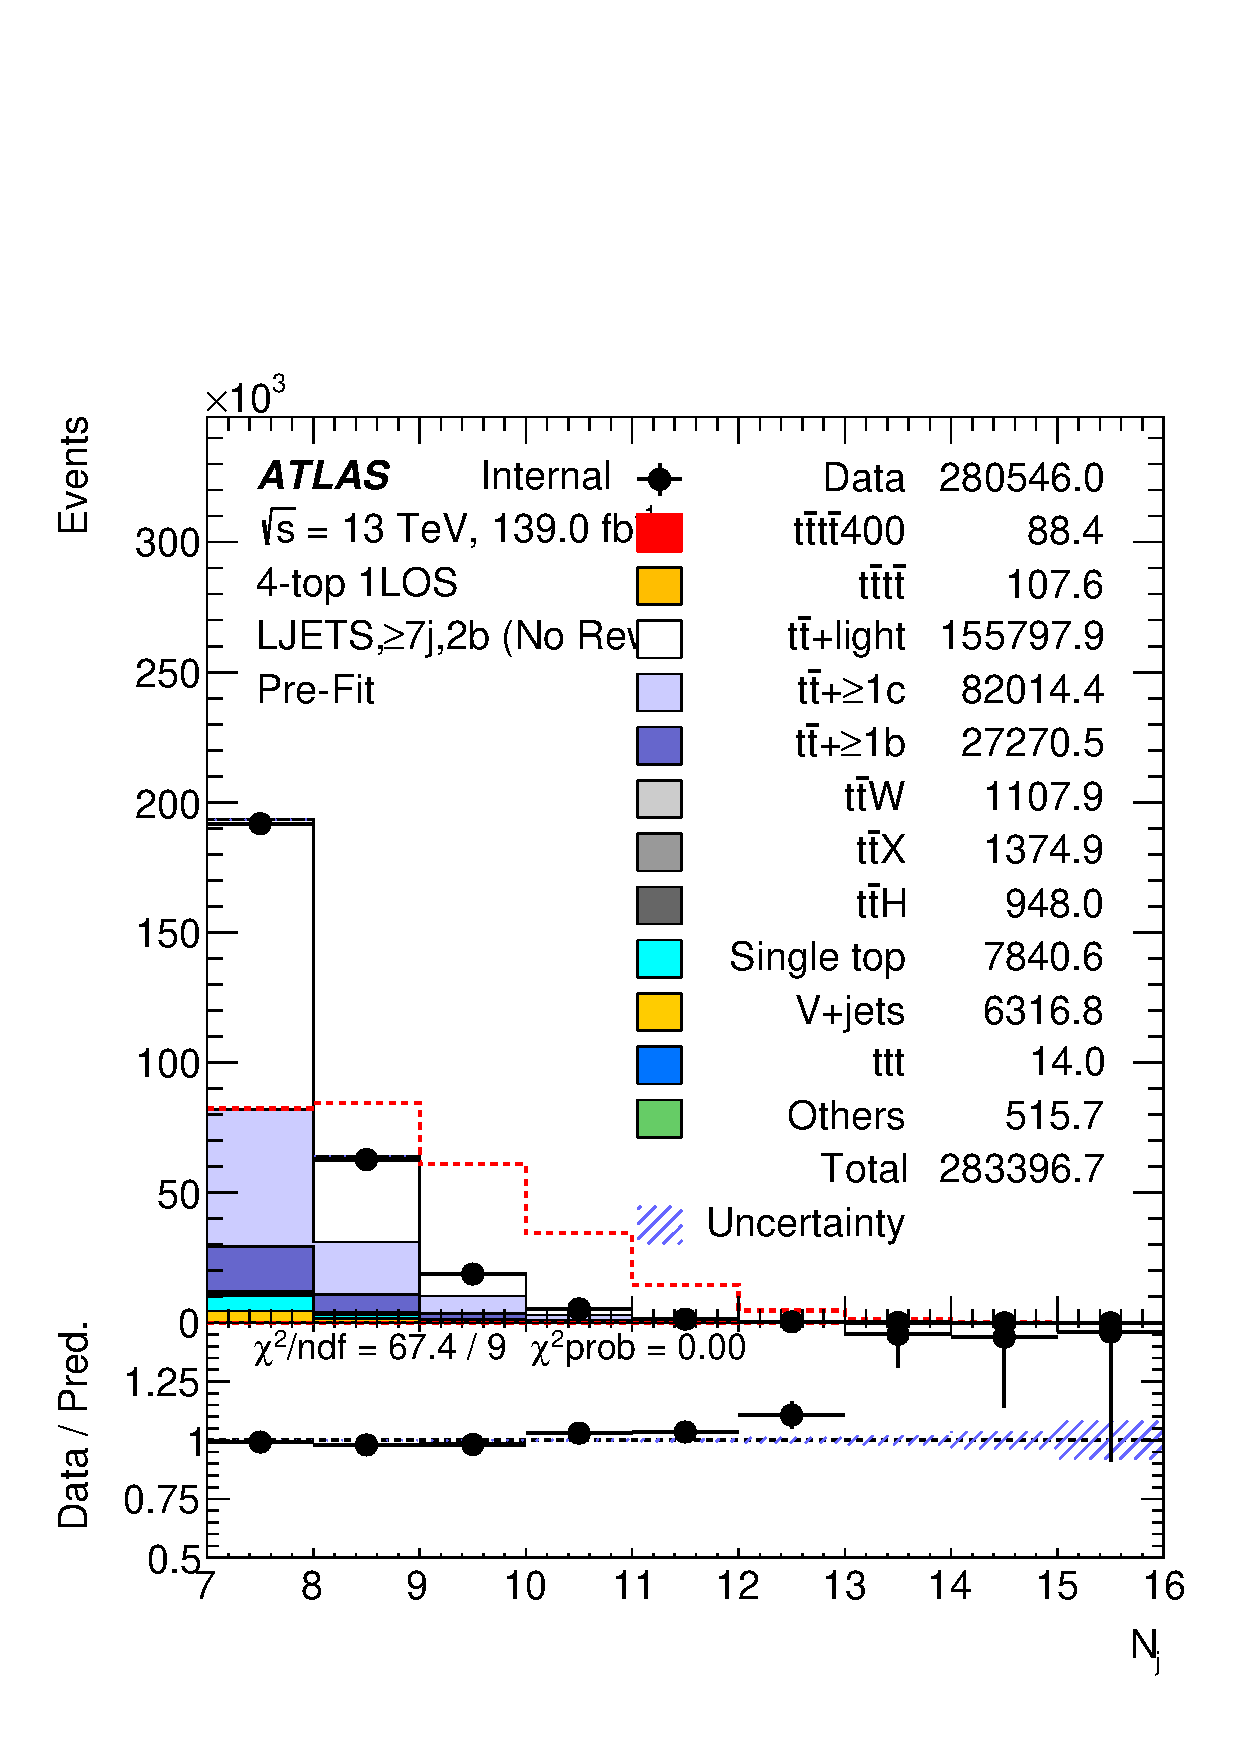
\includegraphics[width=0.4\textwidth]{figures/NNPlots/NNTrainRegion/NoRew/ljets_ge7j2b_nJets.pdf}
    
\includegraphics[width=0.4\textwidth]{figures/NNPlots/NNTrainRegion/Rew/ljets_ge7j2b_nJets.pdf}
    \caption{nJets}
    \end{center}
    \end{subfigure}
    \caption{\label{fig:NNPlots_NNTrainReg_2} The comparison between variables distribution before (left) and after (right) the NN-reweighting in 1L NN training regions ($\geq 7j,=2b$). Blinded regions are excluded.}
\end{figure}

\begin{figure}[htbp!]
    \begin{subfigure}[t]{1\textwidth}
    \begin{center}
    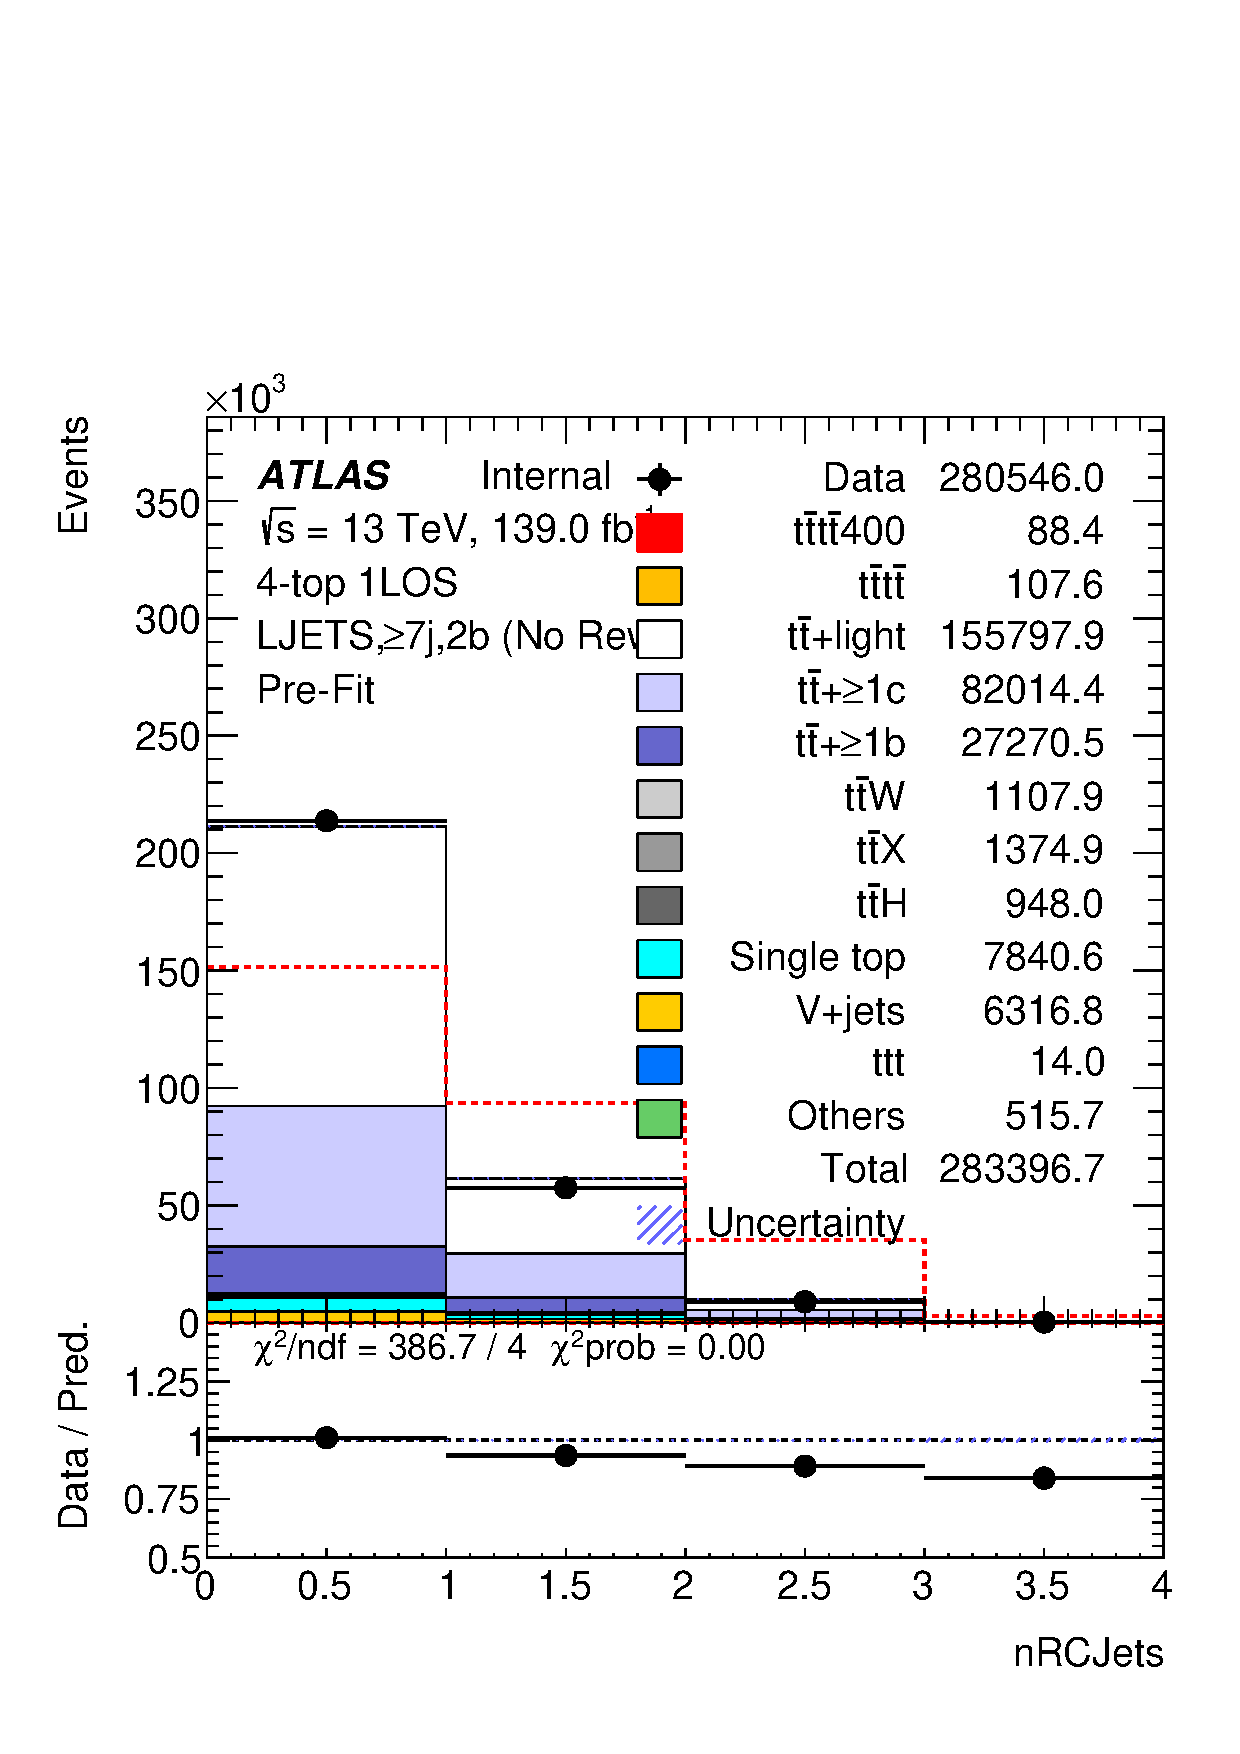
\includegraphics[width=0.4\textwidth]{figures/NNPlots/NNTrainRegion/NoRew/ljets_ge7j2b_nRCJetsM100.pdf}
    
\includegraphics[width=0.4\textwidth]{figures/NNPlots/NNTrainRegion/Rew/ljets_ge7j2b_nRCJetsM100.pdf}
    \caption{nRCJets}
    \end{center}
    \end{subfigure}

    \begin{subfigure}[t]{1\textwidth}
    \begin{center}
    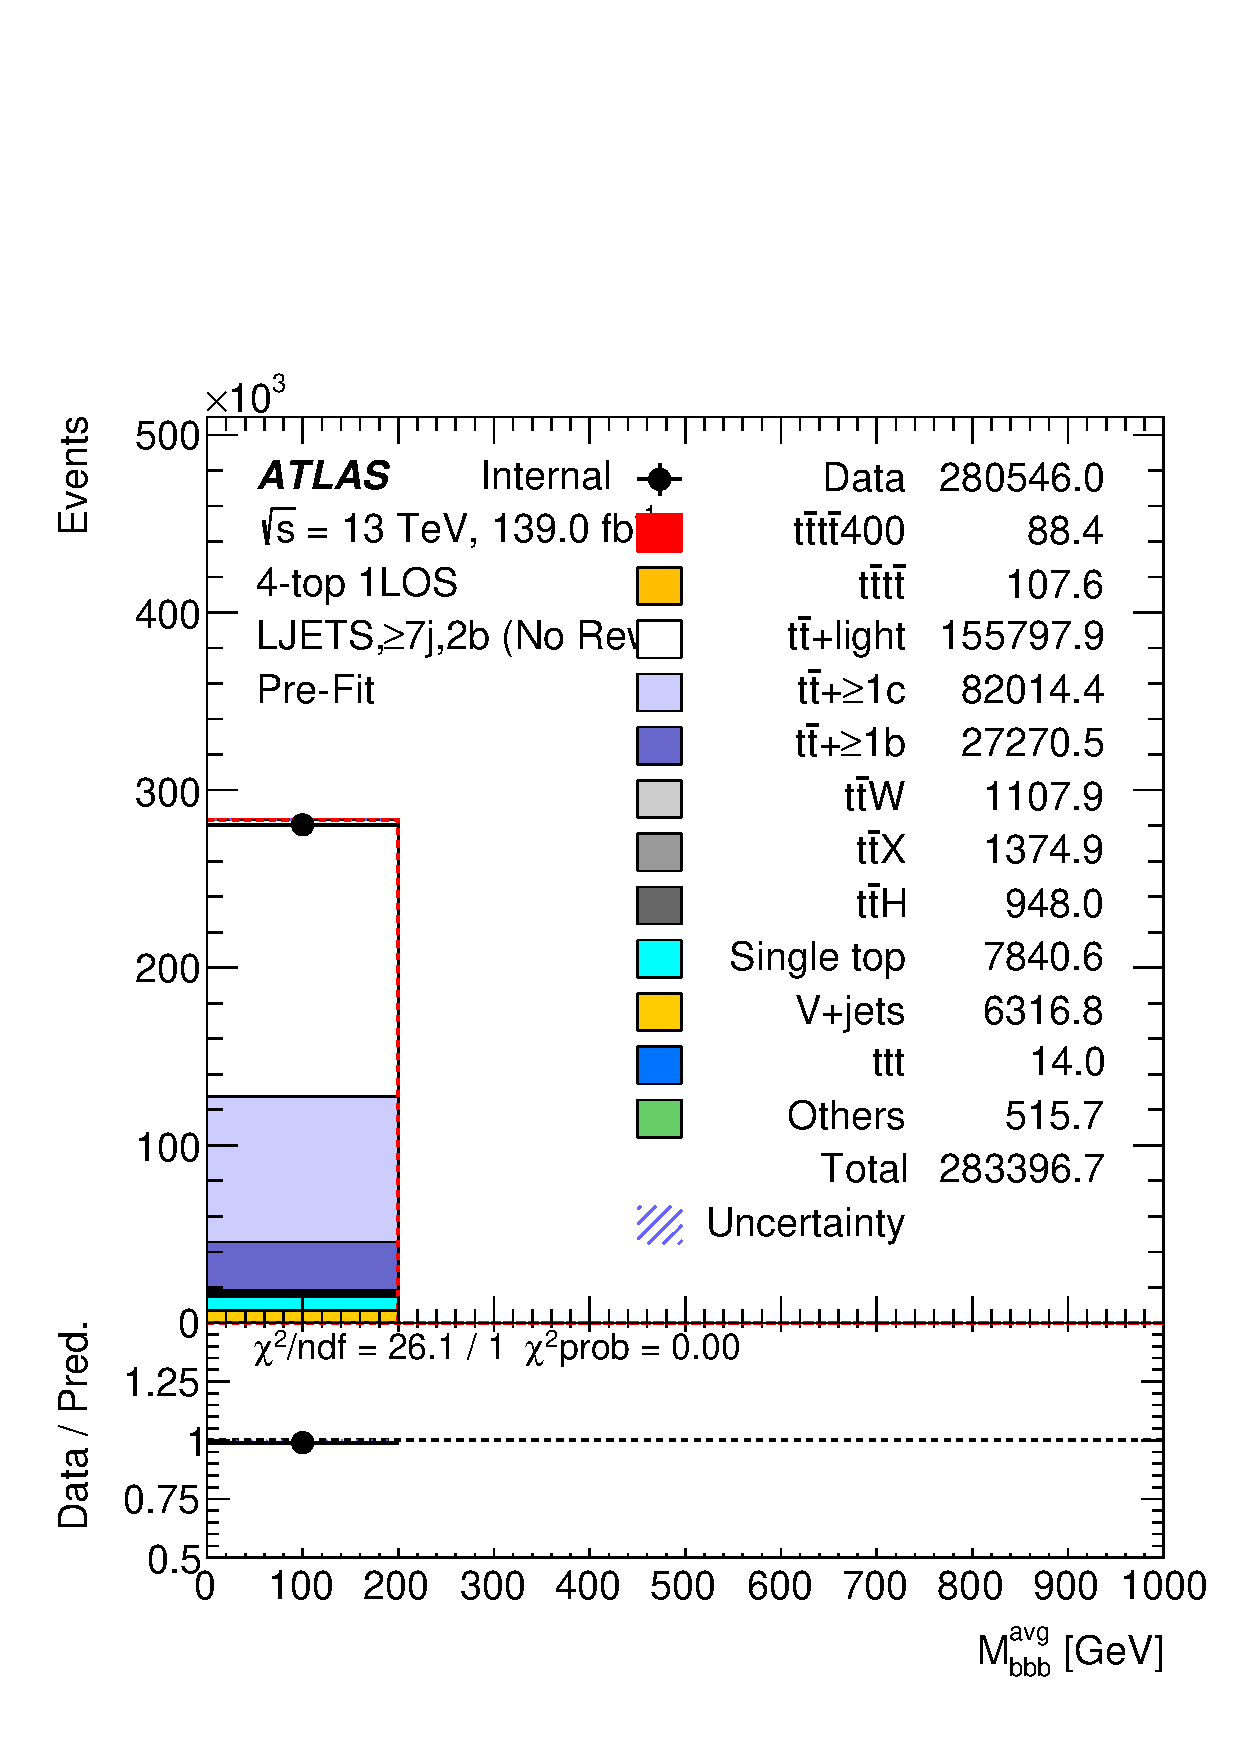
\includegraphics[width=0.4\textwidth]{figures/NNPlots/NNTrainRegion/NoRew/ljets_ge7j2b_Mbbb_Avg_DL1r_70.pdf}
    
\includegraphics[width=0.4\textwidth]{figures/NNPlots/NNTrainRegion/Rew/ljets_ge7j2b_Mbbb_Avg_DL1r_70.pdf}
    \caption{$M^{avg}_{bbb}$}
    \end{center}
    \end{subfigure}

    \begin{subfigure}[t]{1\textwidth}
    \begin{center}
    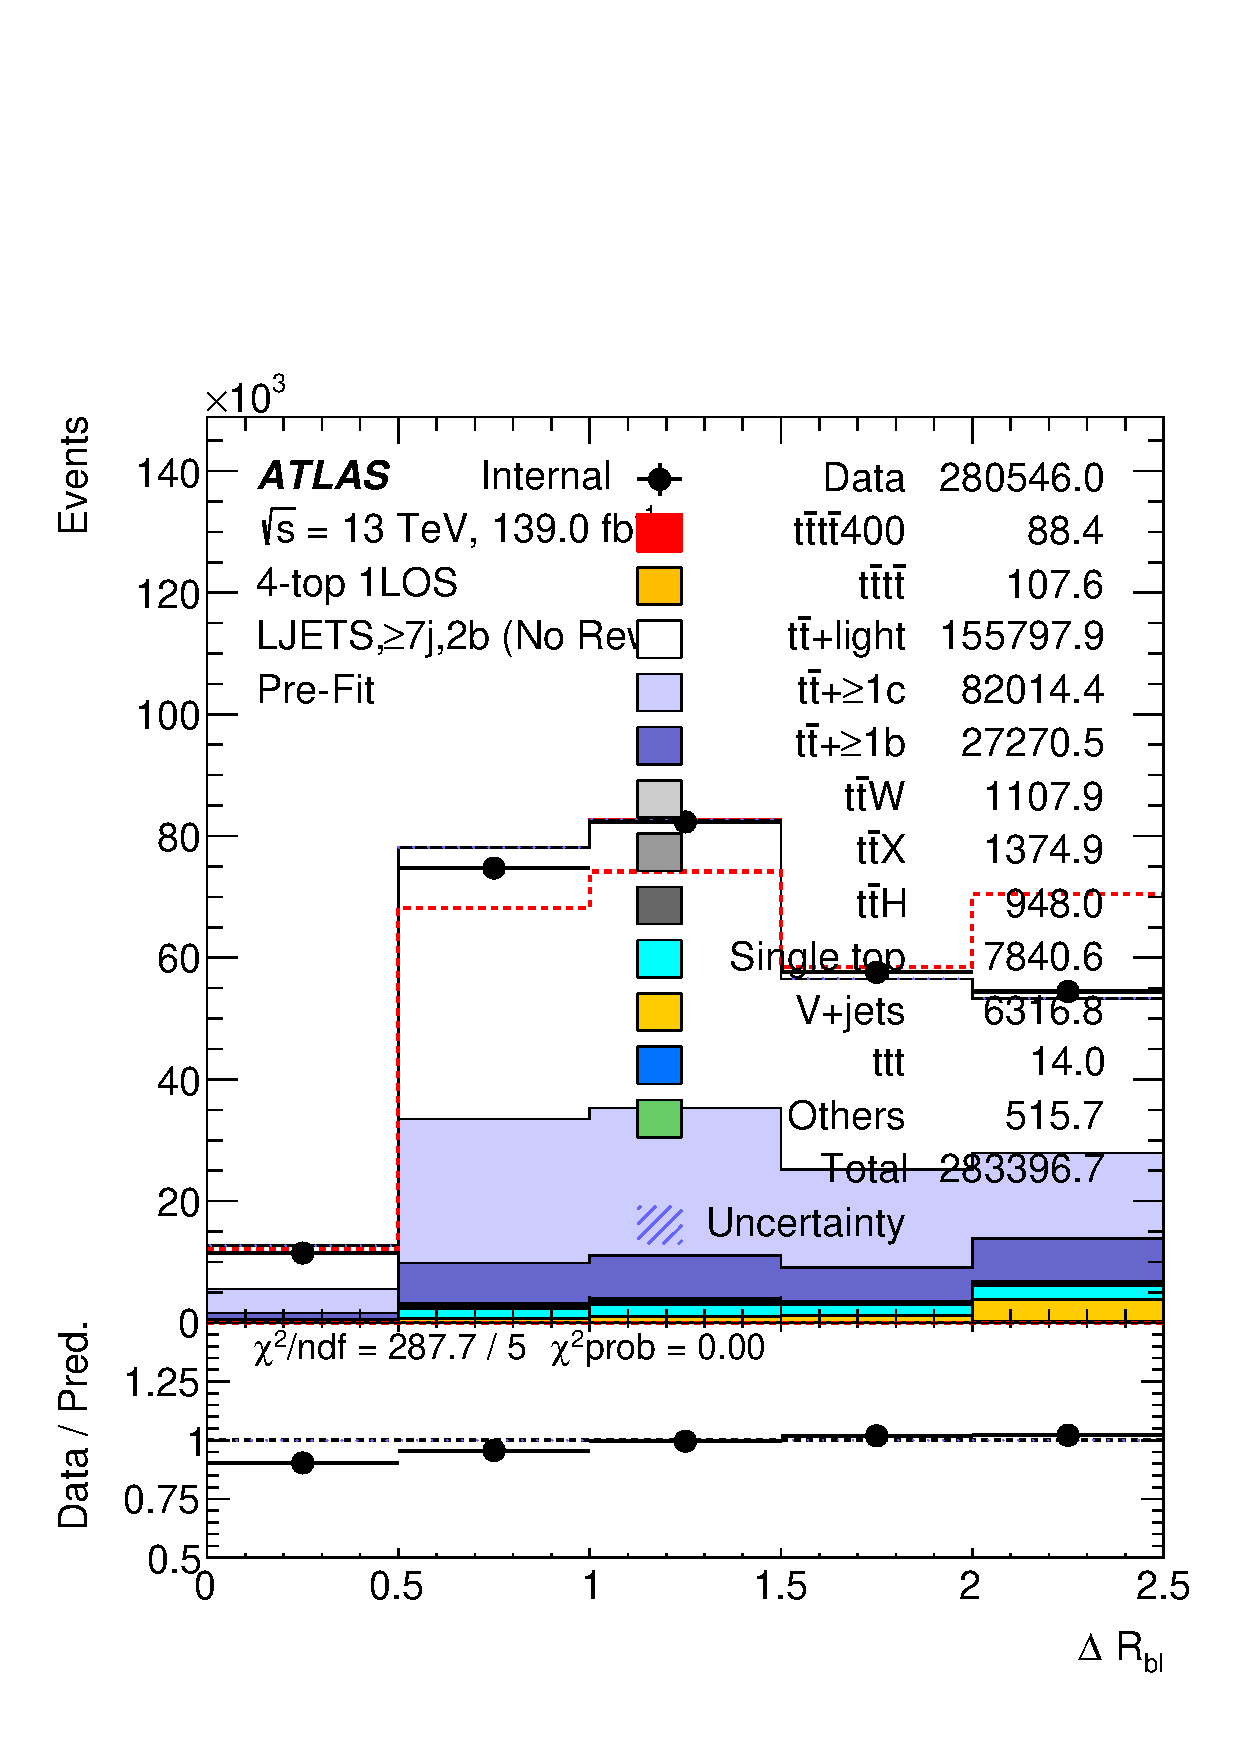
\includegraphics[width=0.4\textwidth]{figures/NNPlots/NNTrainRegion/NoRew/ljets_ge7j2b_dRbl_MindR_DL1r_70.pdf}
    
\includegraphics[width=0.4\textwidth]{figures/NNPlots/NNTrainRegion/Rew/ljets_ge7j2b_dRbl_MindR_DL1r_70.pdf}
    \caption{$\Delta R^{min}_{bl}$}
    \end{center}
    \end{subfigure}
    \caption{\label{fig:NNPlots_NNTrainReg_3} The comparison between variables distribution before (left) and after (right) the NN-reweighting in 1L NN training regions ($\geq 7j,=2b$). Blinded regions are excluded.}
\end{figure}

\begin{figure}[htbp!]
    \begin{subfigure}[t]{1\textwidth}
    \begin{center}
    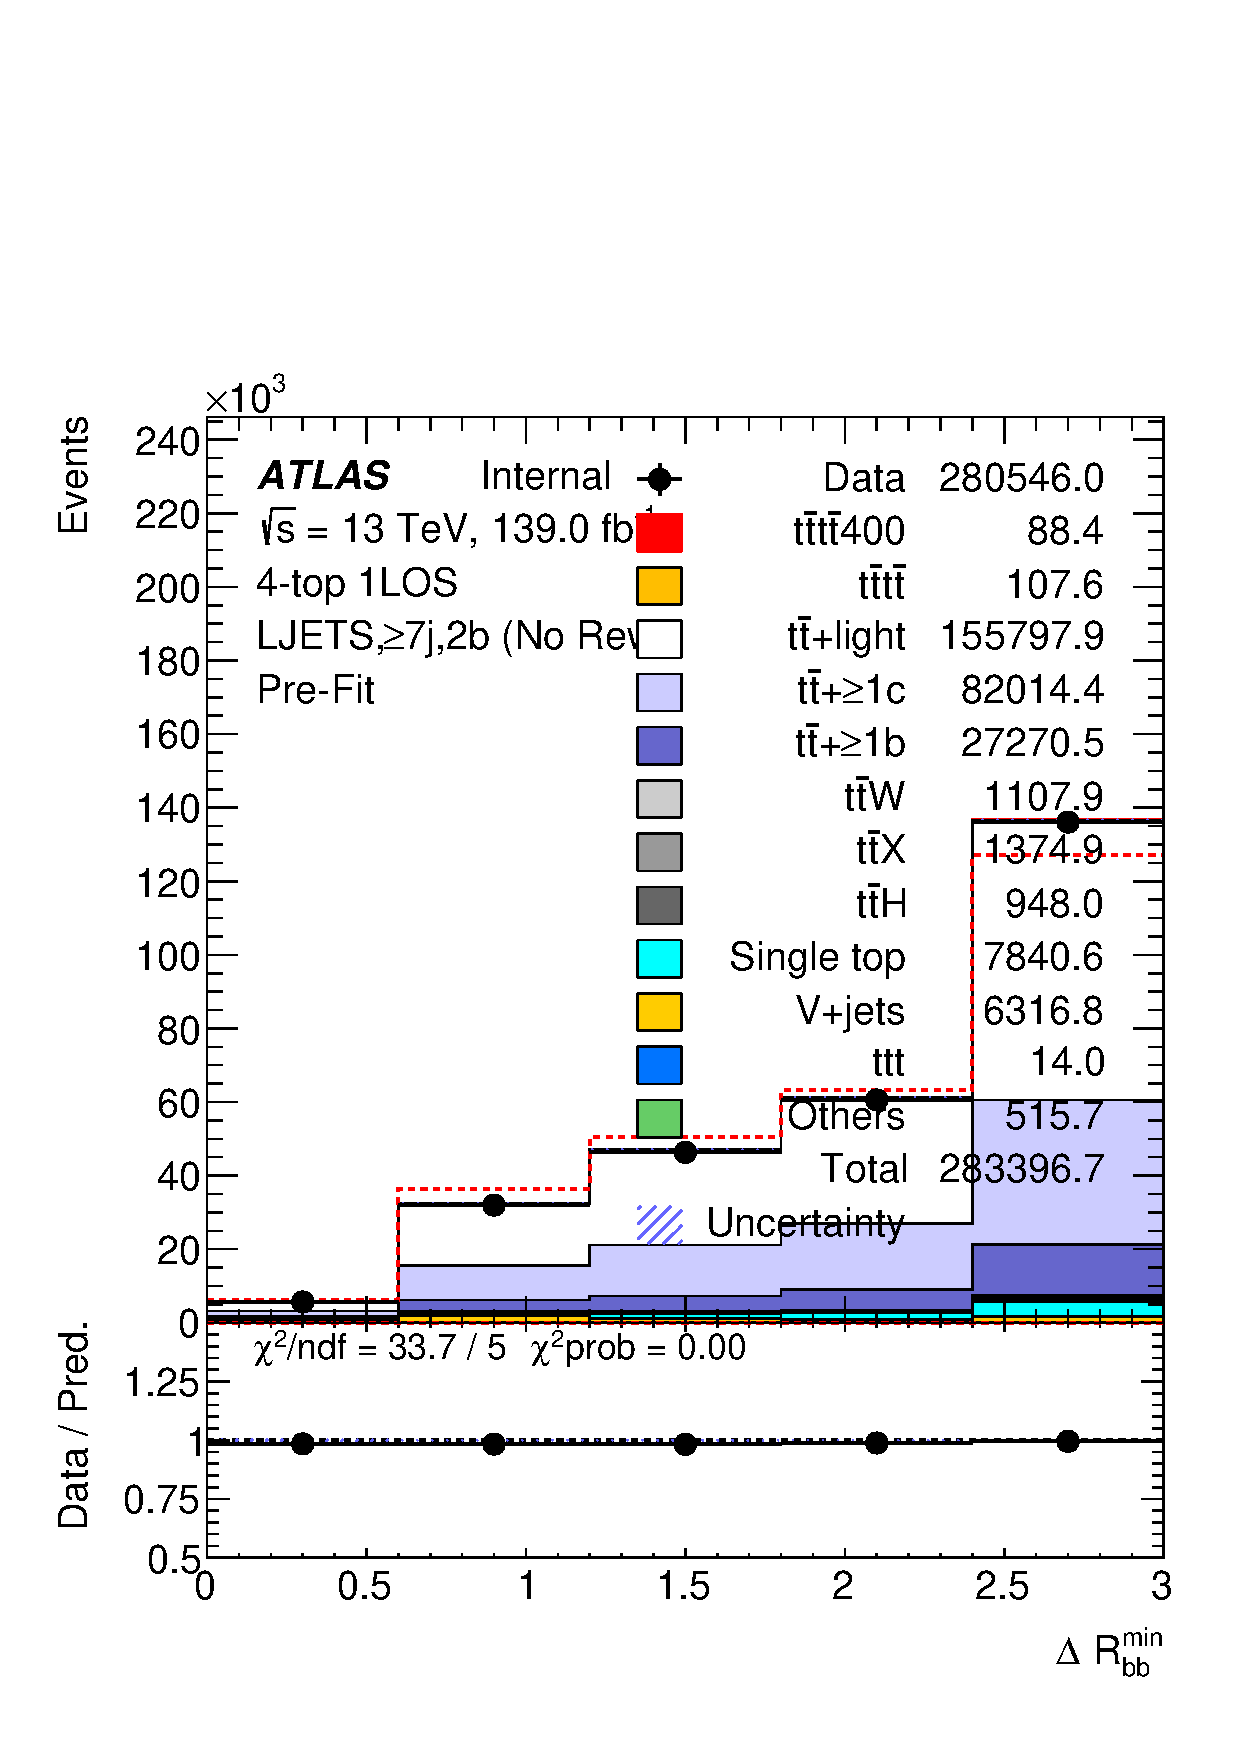
\includegraphics[width=0.4\textwidth]{figures/NNPlots/NNTrainRegion/NoRew/ljets_ge7j2b_dRbb_MindR_DL1r_70.pdf}
    
\includegraphics[width=0.4\textwidth]{figures/NNPlots/NNTrainRegion/Rew/ljets_ge7j2b_dRbb_MindR_DL1r_70.pdf}
    \caption{$\Delta R^{min}_{bb}$}
    \end{center}
    \end{subfigure}

    \begin{subfigure}[t]{1\textwidth}
    \begin{center}
    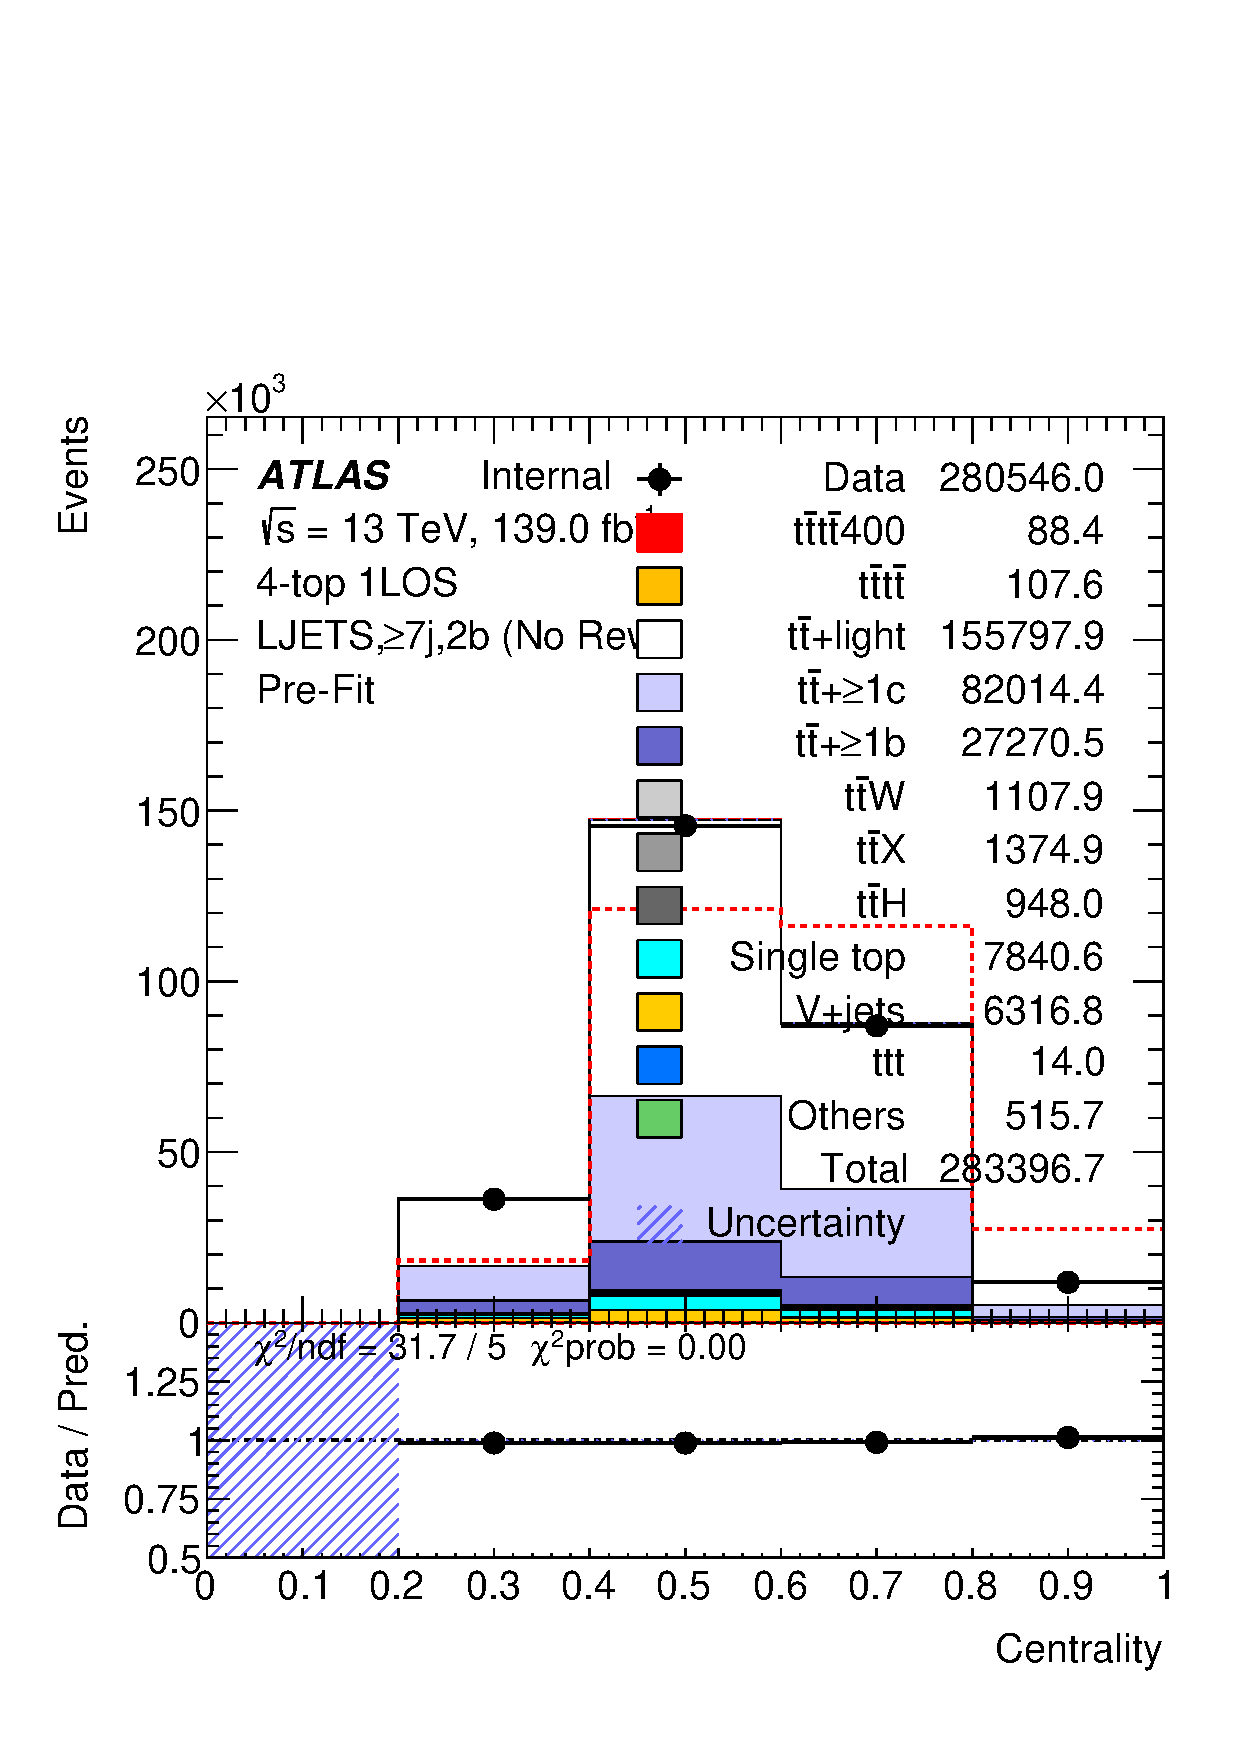
\includegraphics[width=0.4\textwidth]{figures/NNPlots/NNTrainRegion/NoRew/ljets_ge7j2b_Centrality_all.pdf}
    
\includegraphics[width=0.4\textwidth]{figures/NNPlots/NNTrainRegion/Rew/ljets_ge7j2b_Centrality_all.pdf}
    \caption{Centrality}
    \end{center}
    \end{subfigure}

    \begin{subfigure}[t]{1\textwidth}
    \begin{center}
    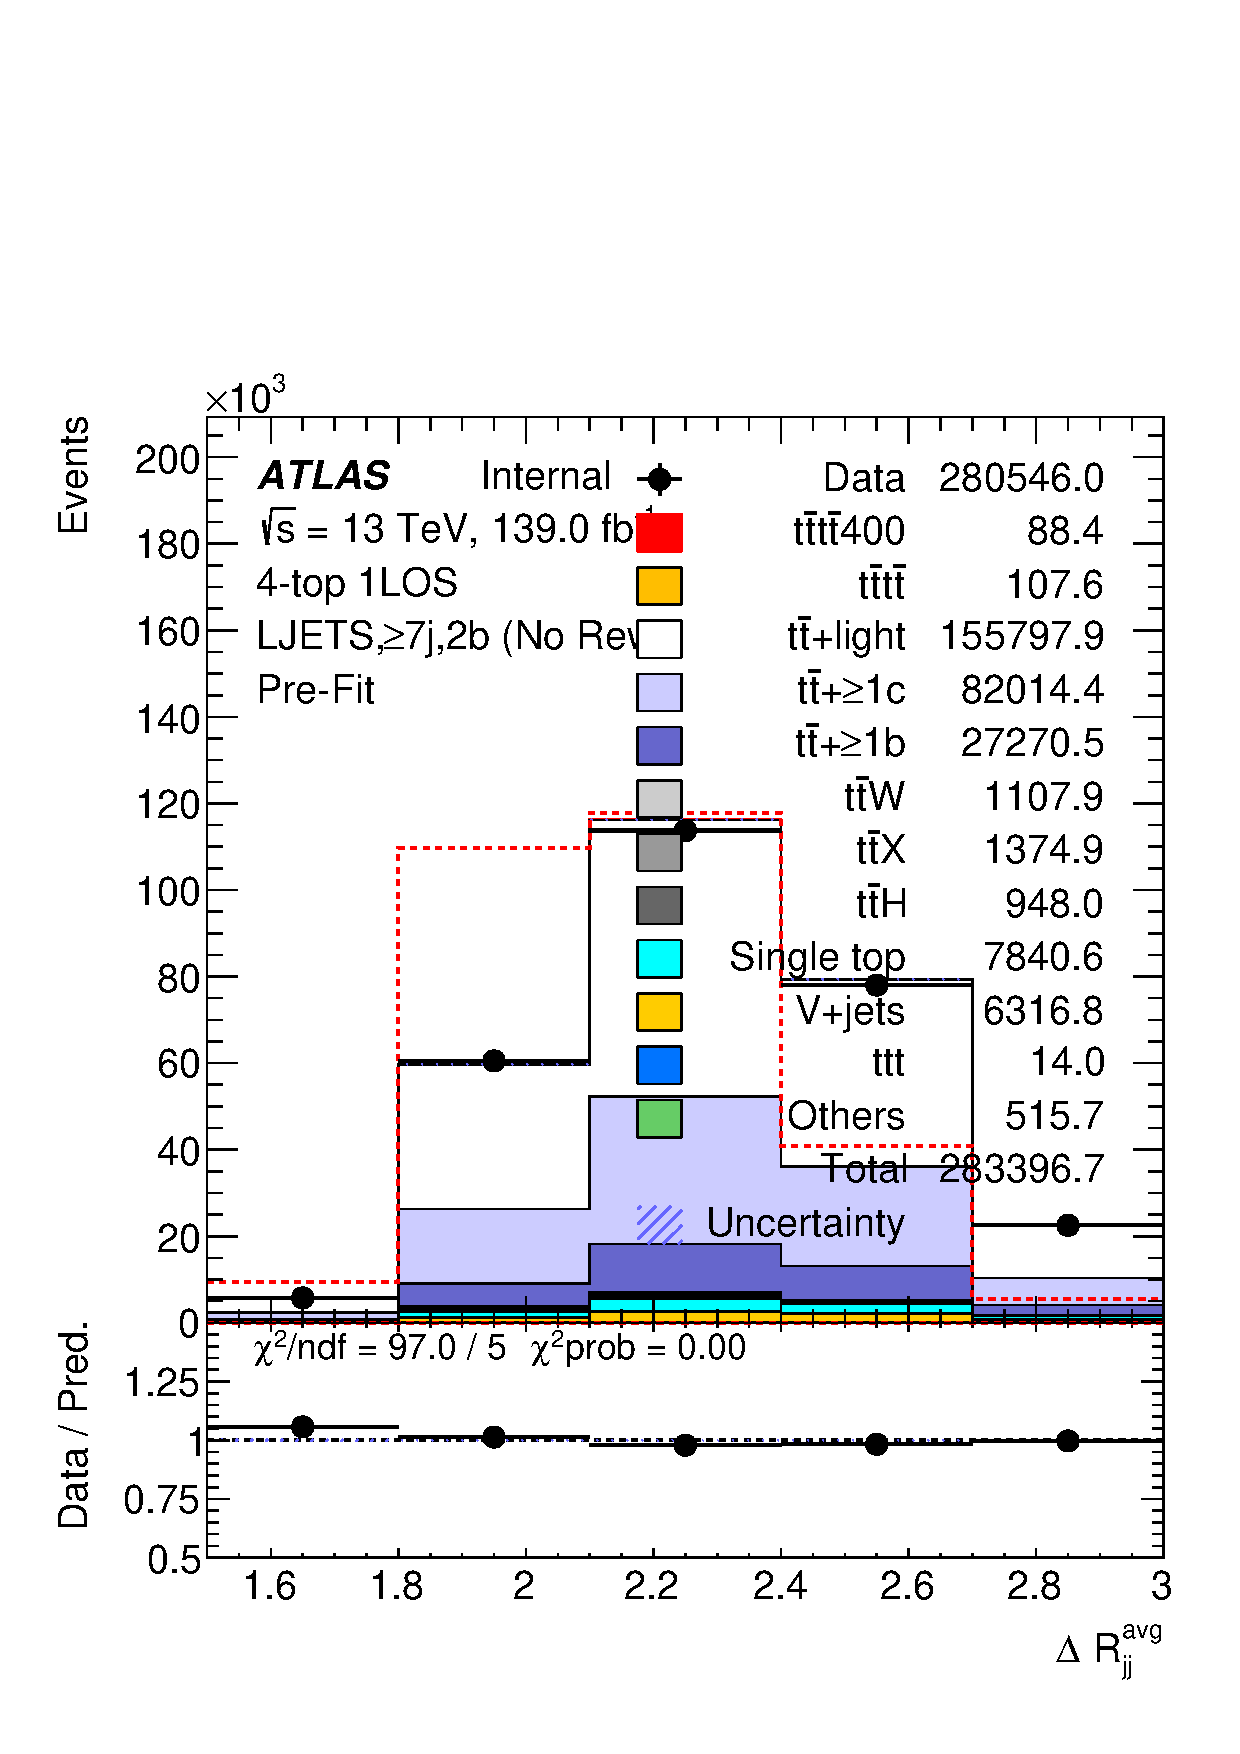
\includegraphics[width=0.4\textwidth]{figures/NNPlots/NNTrainRegion/NoRew/ljets_ge7j2b_dRjj_Avg.pdf}
    
\includegraphics[width=0.4\textwidth]{figures/NNPlots/NNTrainRegion/Rew/ljets_ge7j2b_dRjj_Avg.pdf}
    \caption{$\Delta R^{avg}_{jj}$}
    \end{center}
    \end{subfigure}
    \caption{\label{fig:NNPlots_NNTrainReg_4} The comparison between variables distribution before (left) and after (right) the NN-reweighting in 1L NN training regions ($\geq 7j,=2b$). Blinded regions are excluded.}
\end{figure}

\begin{figure}[htbp!]
    \begin{subfigure}[t]{1\textwidth}
    \begin{center}
    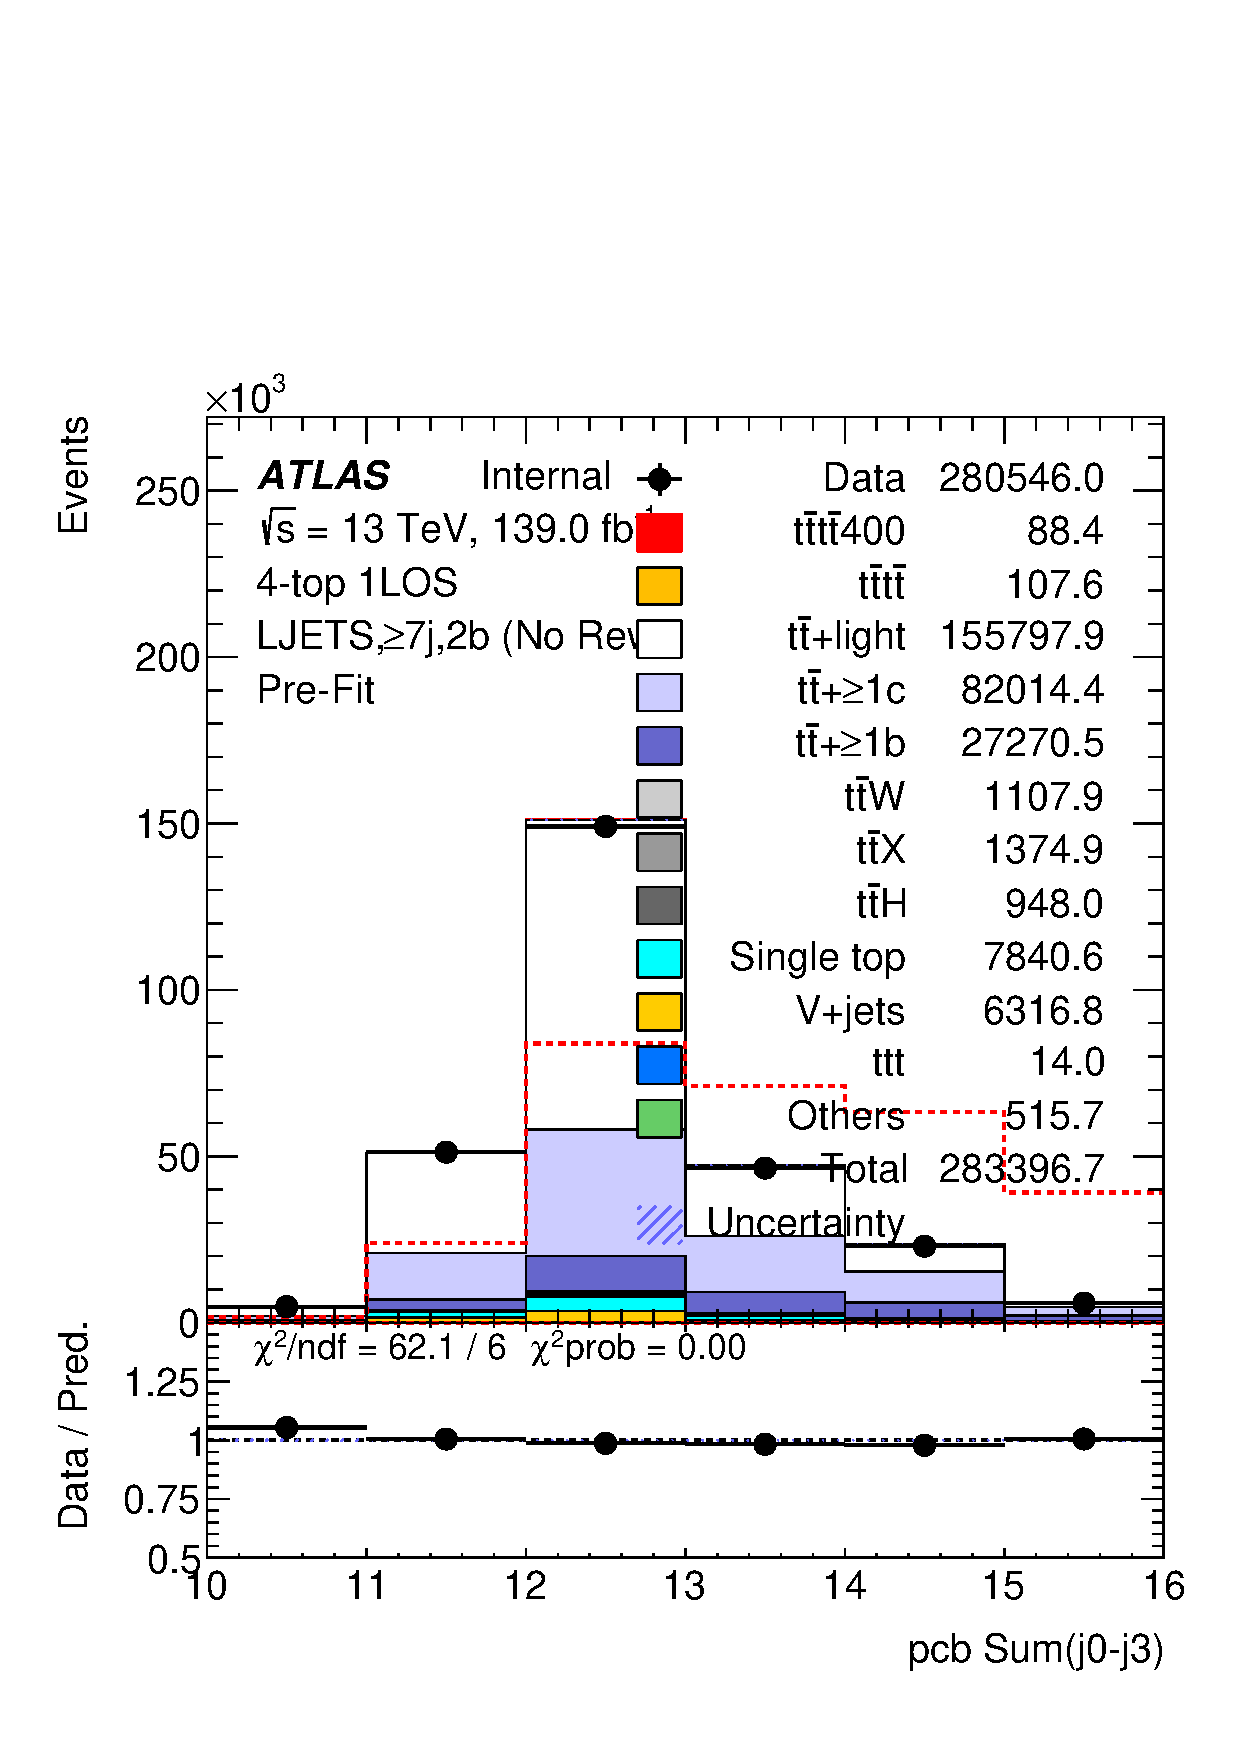
\includegraphics[width=0.4\textwidth]{figures/NNPlots/NNTrainRegion/NoRew/ljets_ge7j2b_pcb.pdf}
    
\includegraphics[width=0.4\textwidth]{figures/NNPlots/NNTrainRegion/Rew/ljets_ge7j2b_pcb.pdf}
    \caption{pcb Sum}
    \end{center}
    \end{subfigure}

    \begin{subfigure}[t]{1\textwidth}
    \begin{center}
    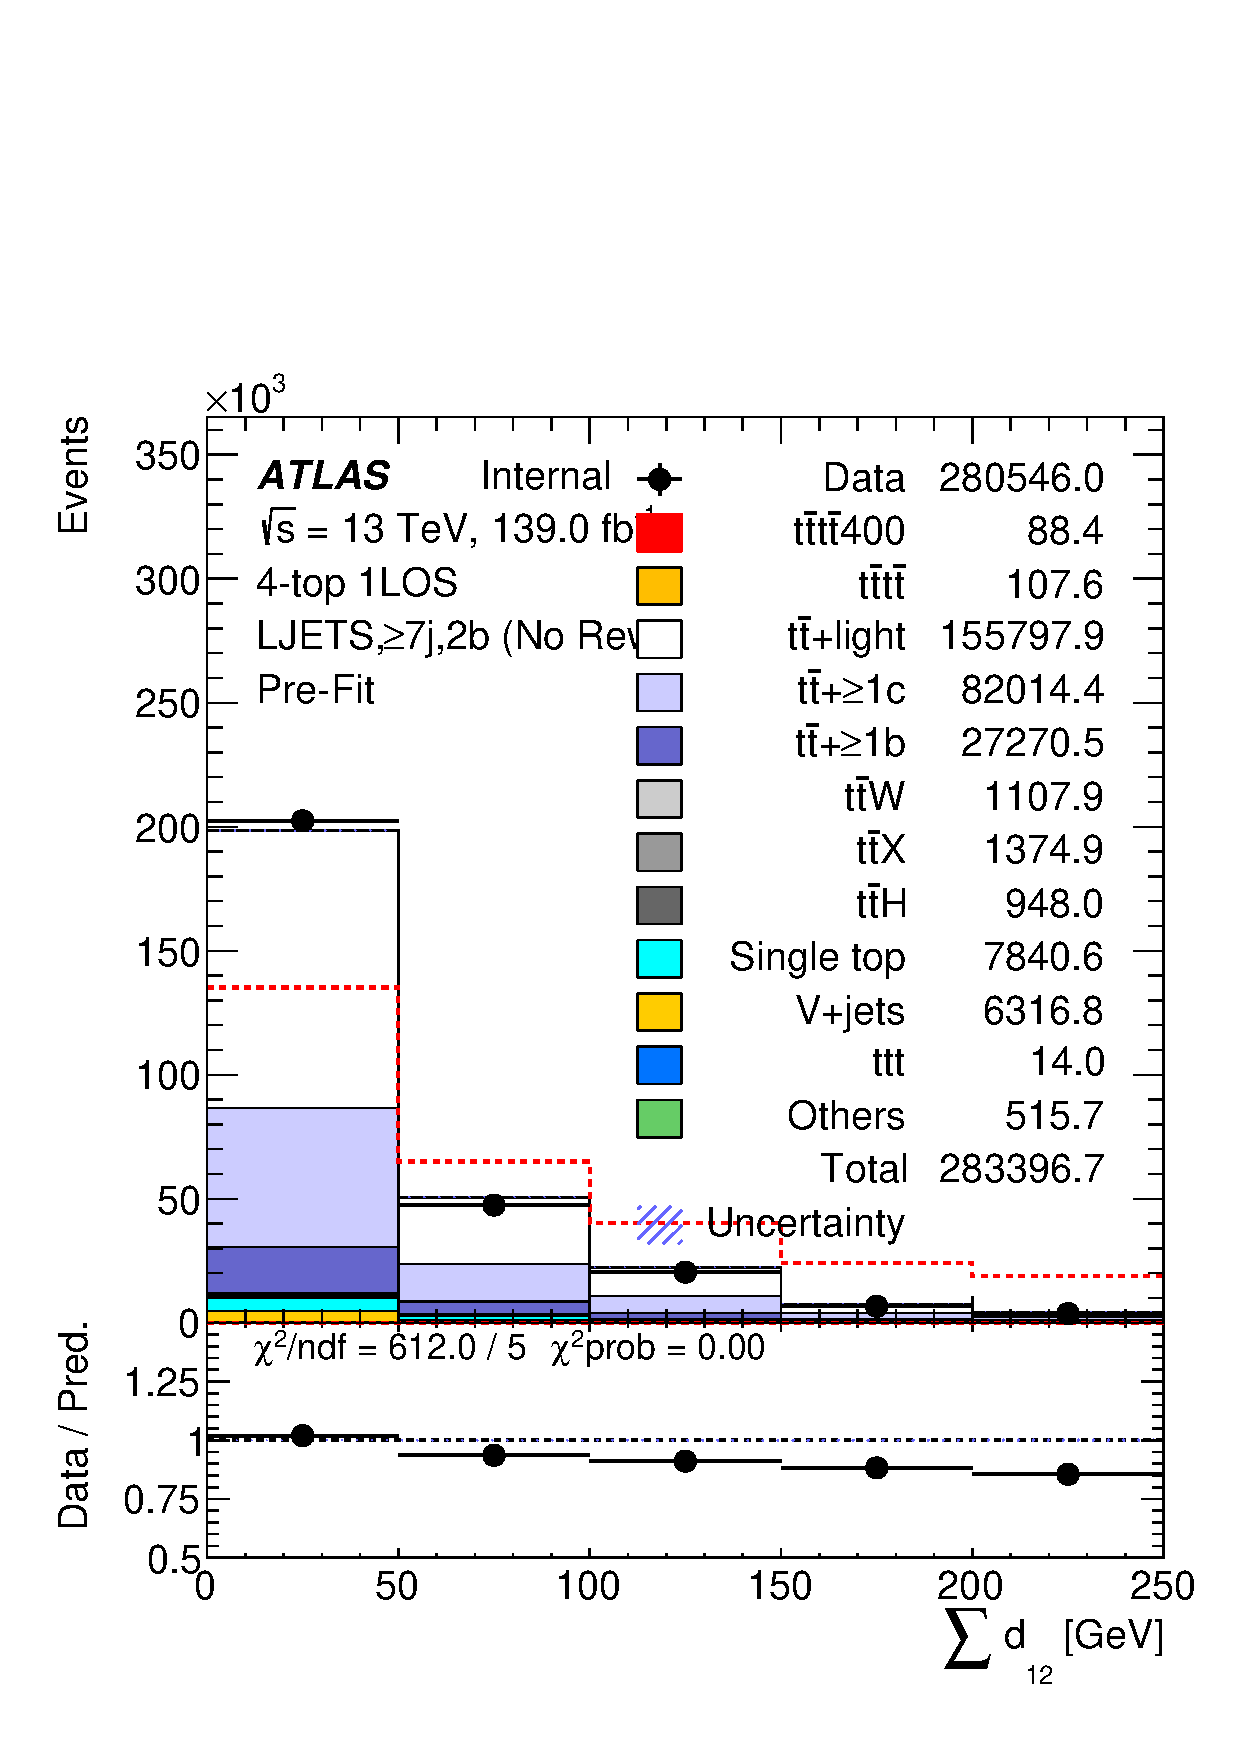
\includegraphics[width=0.4\textwidth]{figures/NNPlots/NNTrainRegion/NoRew/ljets_ge7j2b_sum_d12.pdf}
    
\includegraphics[width=0.4\textwidth]{figures/NNPlots/NNTrainRegion/Rew/ljets_ge7j2b_sum_d12.pdf}
    \caption{$\sum d_{12}$}
    \end{center}
    \end{subfigure}

    \begin{subfigure}[t]{1\textwidth}
    \begin{center}
    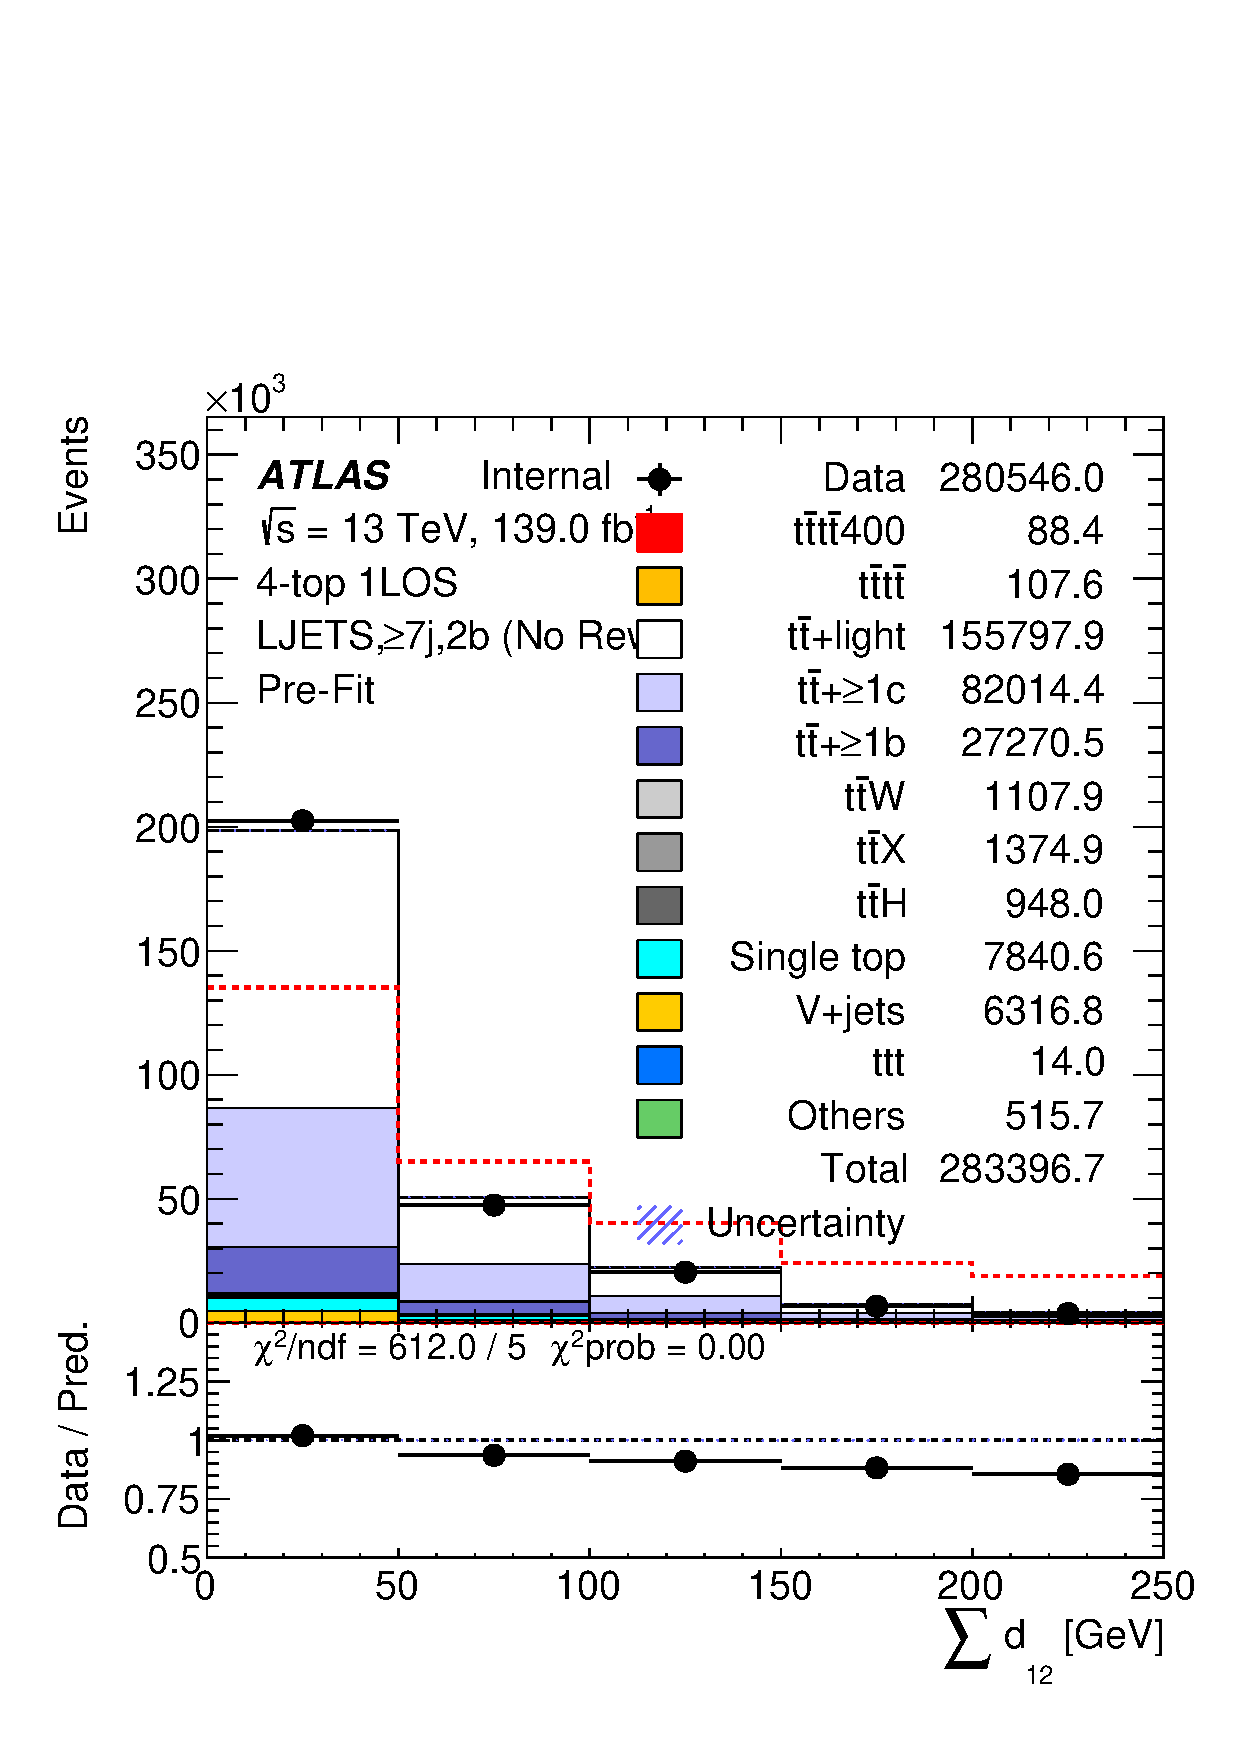
\includegraphics[width=0.4\textwidth]{figures/NNPlots/NNTrainRegion/NoRew/ljets_ge7j2b_sum_d23.pdf}
    
\includegraphics[width=0.4\textwidth]{figures/NNPlots/NNTrainRegion/Rew/ljets_ge7j2b_sum_d23.pdf}
    \caption{$\sum d_{23}$}
    \end{center}
    \end{subfigure}
    \caption{\label{fig:NNPlots_NNTrainReg_5} The comparison between variables distribution before (left) and after (right) the NN-reweighting in 1L NN training regions ($\geq 7j,=2b$). Blinded regions are excluded.}
\end{figure}

%%% 2LOS %%%
\begin{figure}[htbp!]
    \begin{subfigure}[t]{1\textwidth}
    \begin{center}
    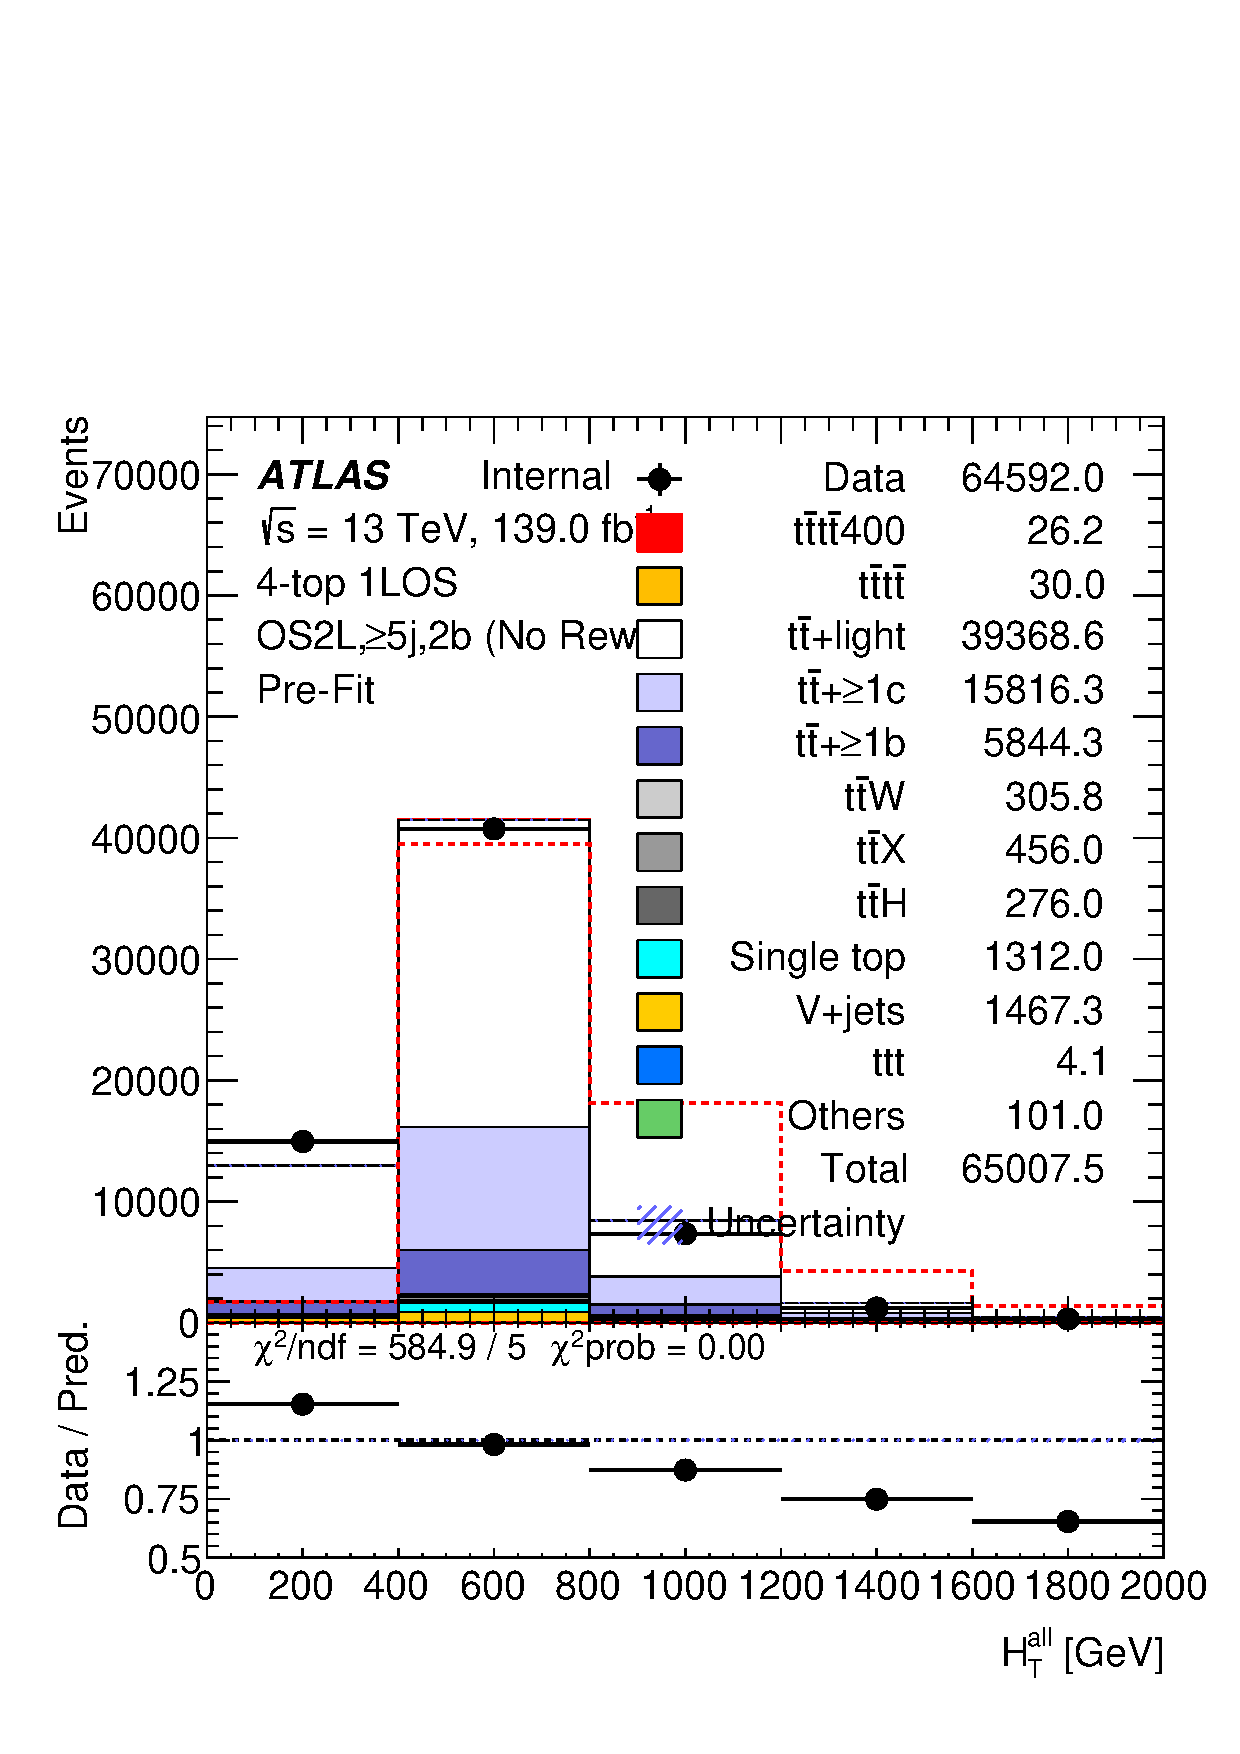
\includegraphics[width=0.4\textwidth]{figures/NNPlots/NNTrainRegion/NoRew/os2l_ge5j2b_HT.pdf}
    
\includegraphics[width=0.4\textwidth]{figures/NNPlots/NNTrainRegion/Rew/os2l_ge5j2b_HT.pdf}
    \caption{$H_{T}$}
    \end{center}
    \end{subfigure}

    \begin{subfigure}[t]{1\textwidth}
    \begin{center}
    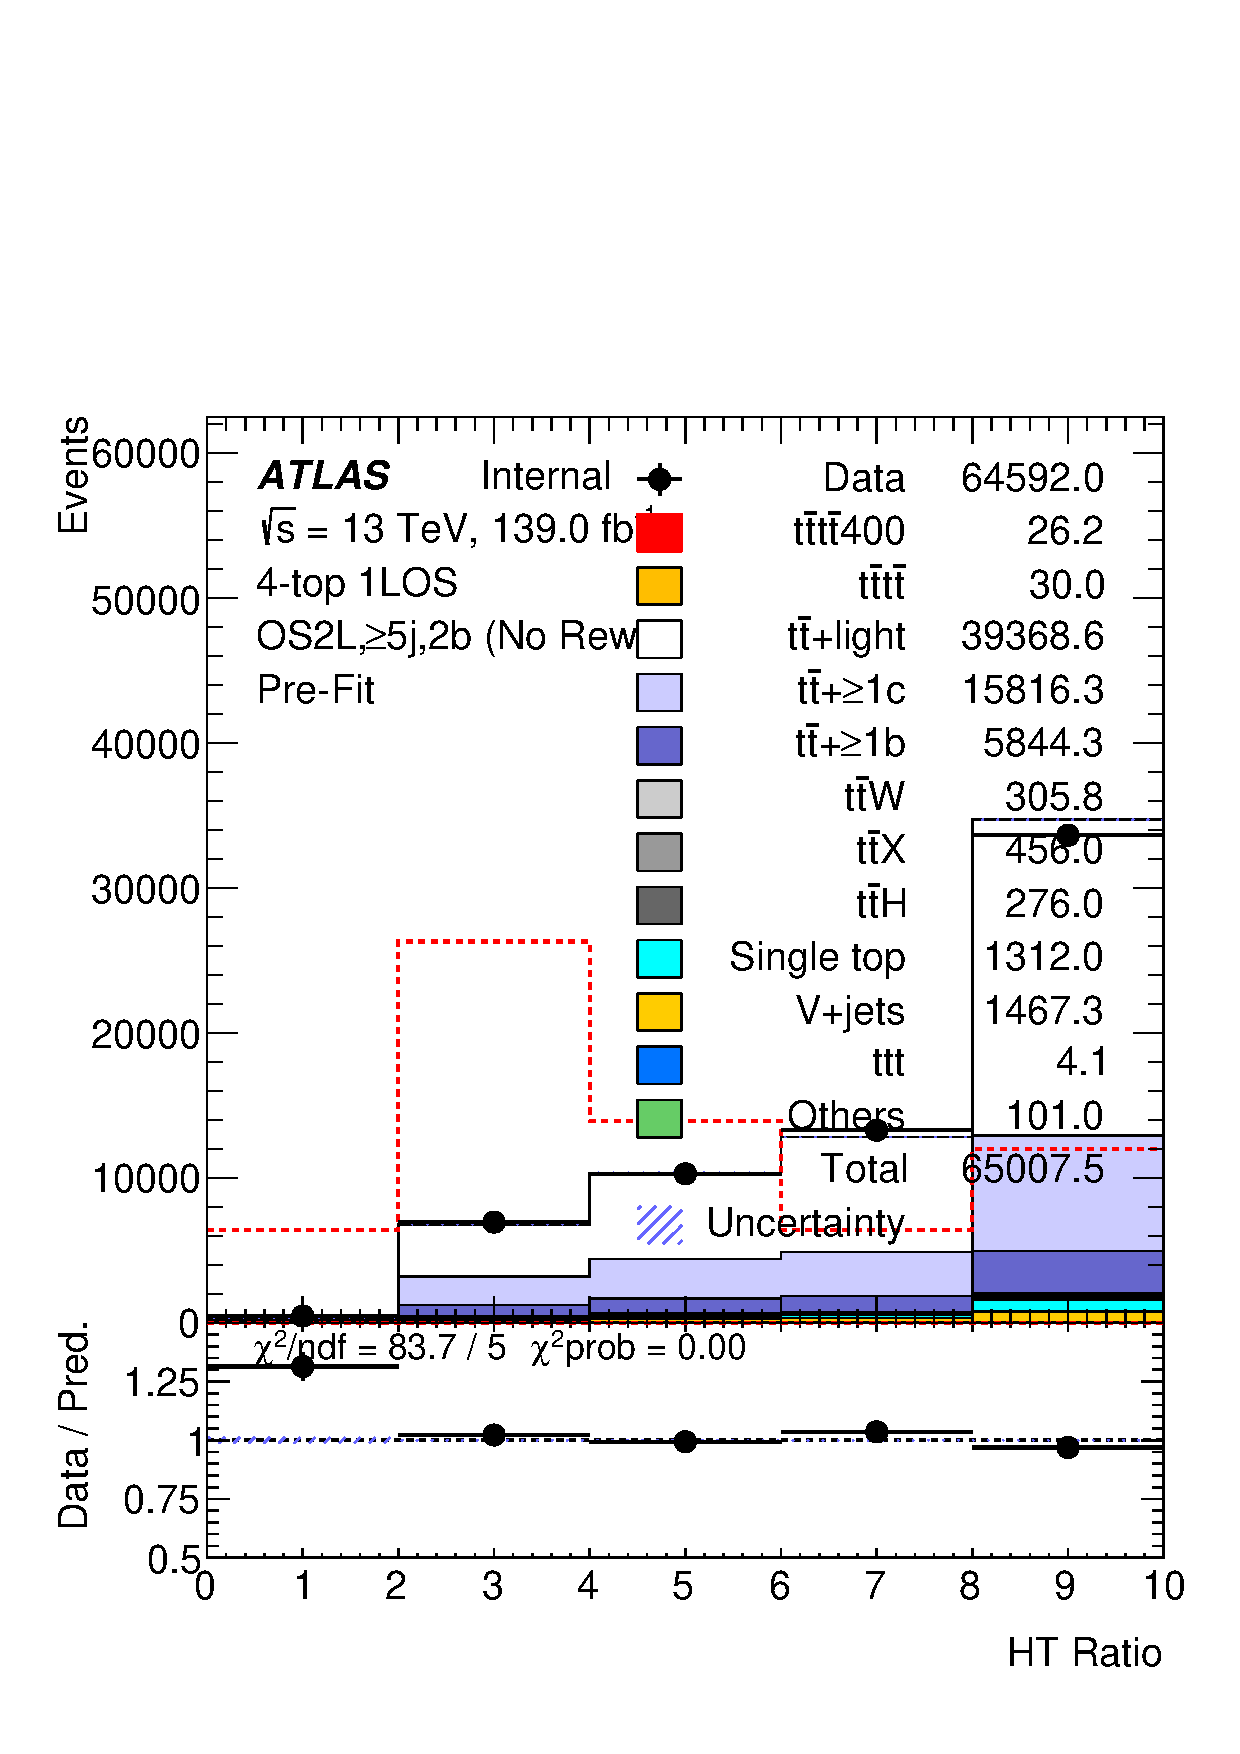
\includegraphics[width=0.4\textwidth]{figures/NNPlots/NNTrainRegion/NoRew/os2l_ge5j2b_HTRatio.pdf}
    
\includegraphics[width=0.4\textwidth]{figures/NNPlots/NNTrainRegion/Rew/os2l_ge5j2b_HTRatio.pdf}
    \caption{HTRatio}
    \end{center}
    \end{subfigure}

    \begin{subfigure}[t]{1\textwidth}
    \begin{center}
    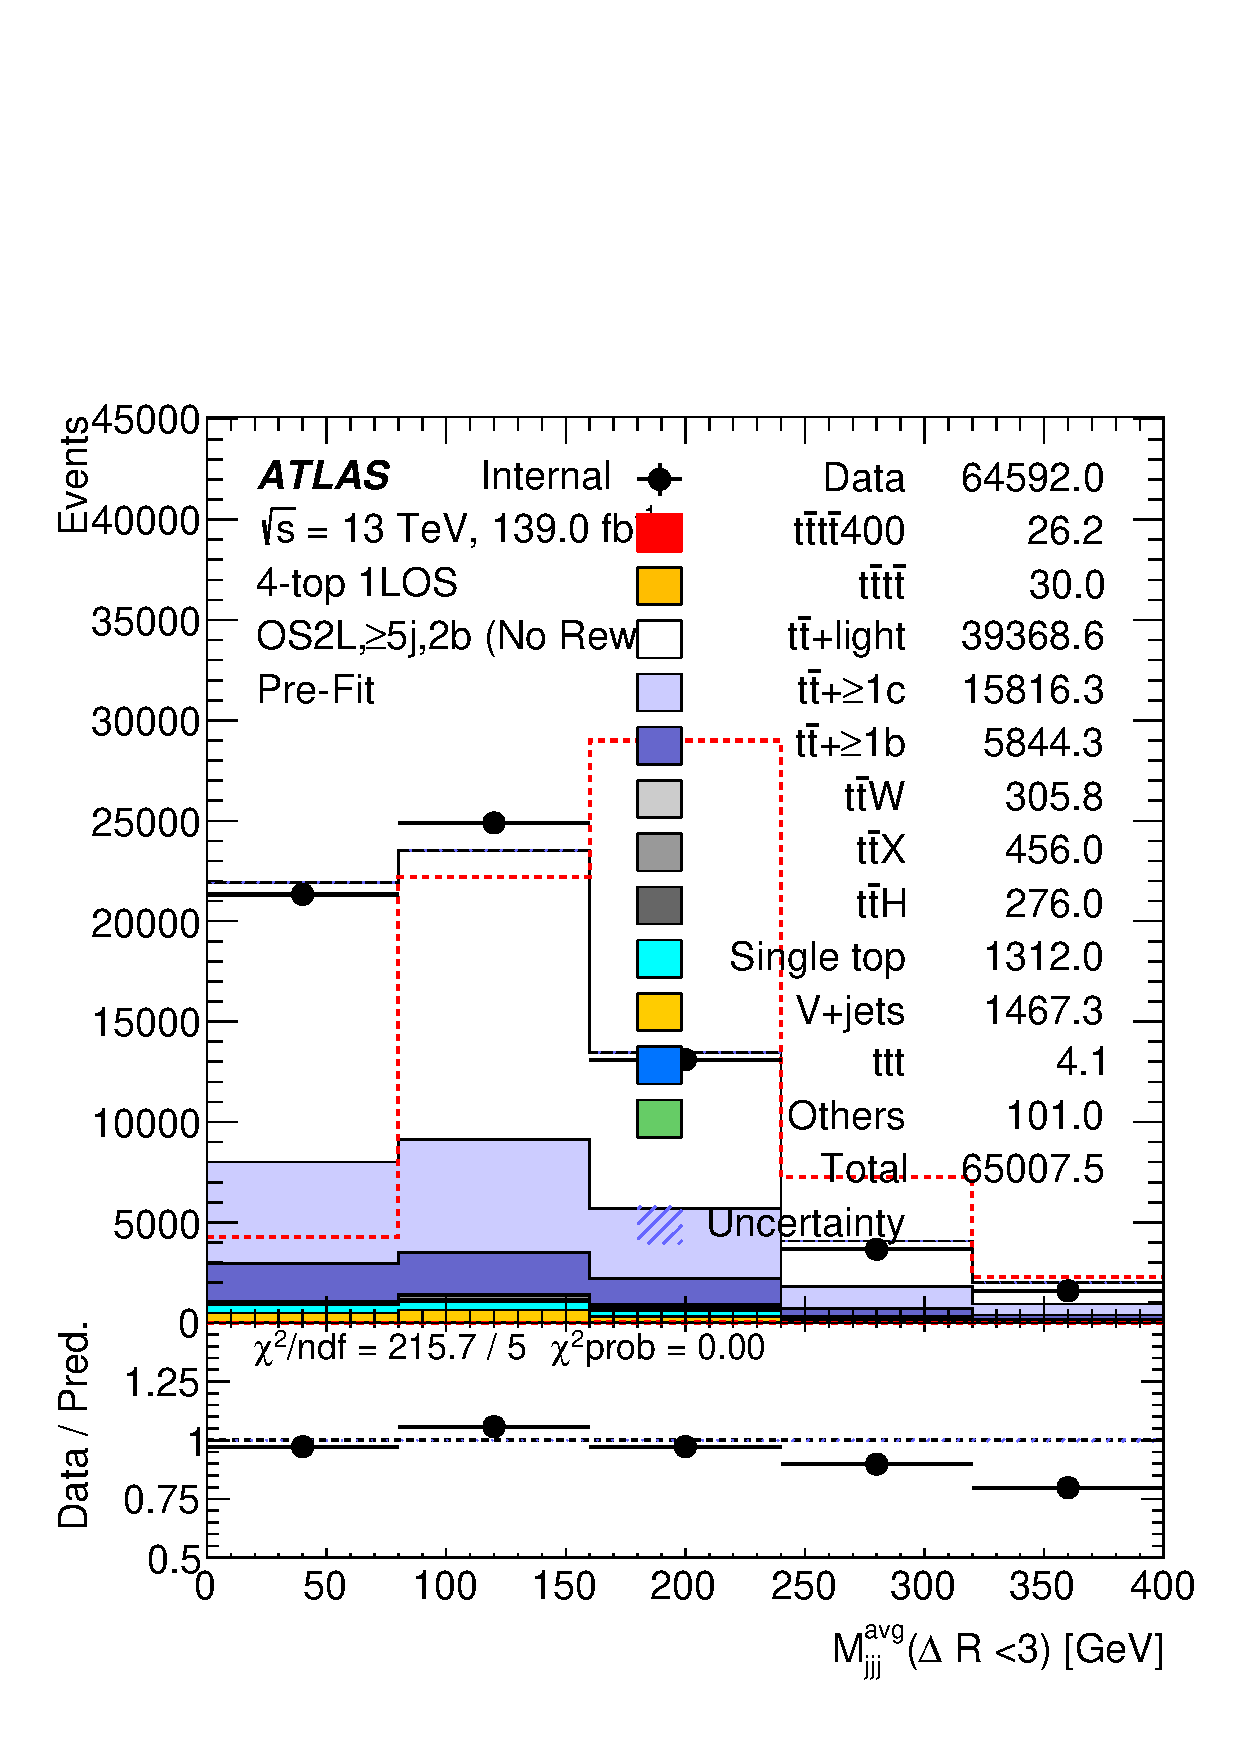
\includegraphics[width=0.4\textwidth]{figures/NNPlots/NNTrainRegion/NoRew/os2l_ge5j2b_Mjjj_AvgdRs3.pdf}
    
\includegraphics[width=0.4\textwidth]{figures/NNPlots/NNTrainRegion/Rew/os2l_ge5j2b_Mjjj_AvgdRs3.pdf}
    \caption{$M^{avg}_{jjj}(\Delta R <3)$}
    \end{center}
    \end{subfigure}
    \caption{\label{fig:NNPlots_NNTrainReg_6} The comparison between variables distribution before (left) and after (right) the NN-reweighting in 1L NN training regions ($\geq 5j,=2b$). Blinded regions are excluded.}  
\end{figure}

\begin{figure}[htbp!]
    \begin{subfigure}[t]{1\textwidth}
    \begin{center}
    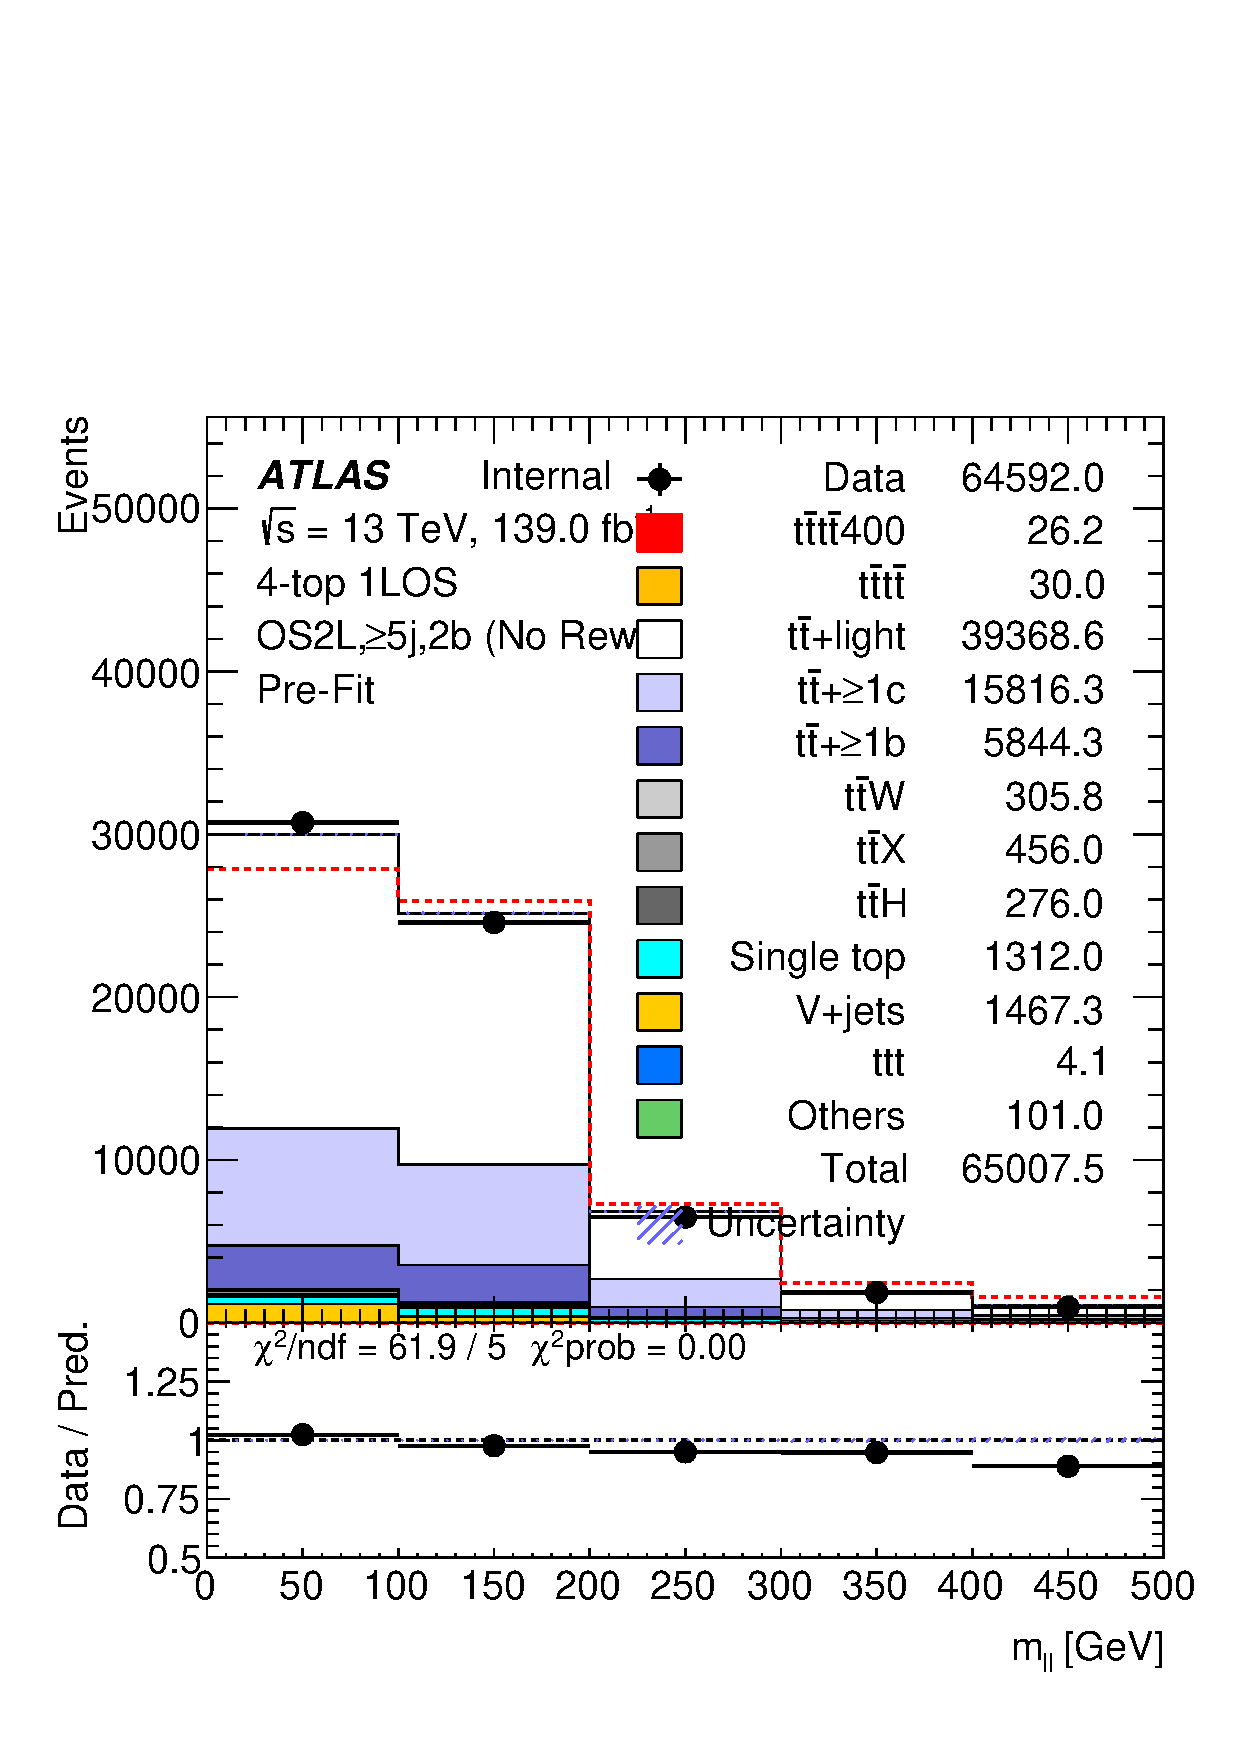
\includegraphics[width=0.4\textwidth]{figures/NNPlots/NNTrainRegion/NoRew/os2l_ge5j2b_mll.pdf}
    
\includegraphics[width=0.4\textwidth]{figures/NNPlots/NNTrainRegion/Rew/os2l_ge5j2b_mll.pdf}
    \caption{mll}
    \end{center}
    \end{subfigure}

    \begin{subfigure}[t]{1\textwidth}
    \begin{center}
    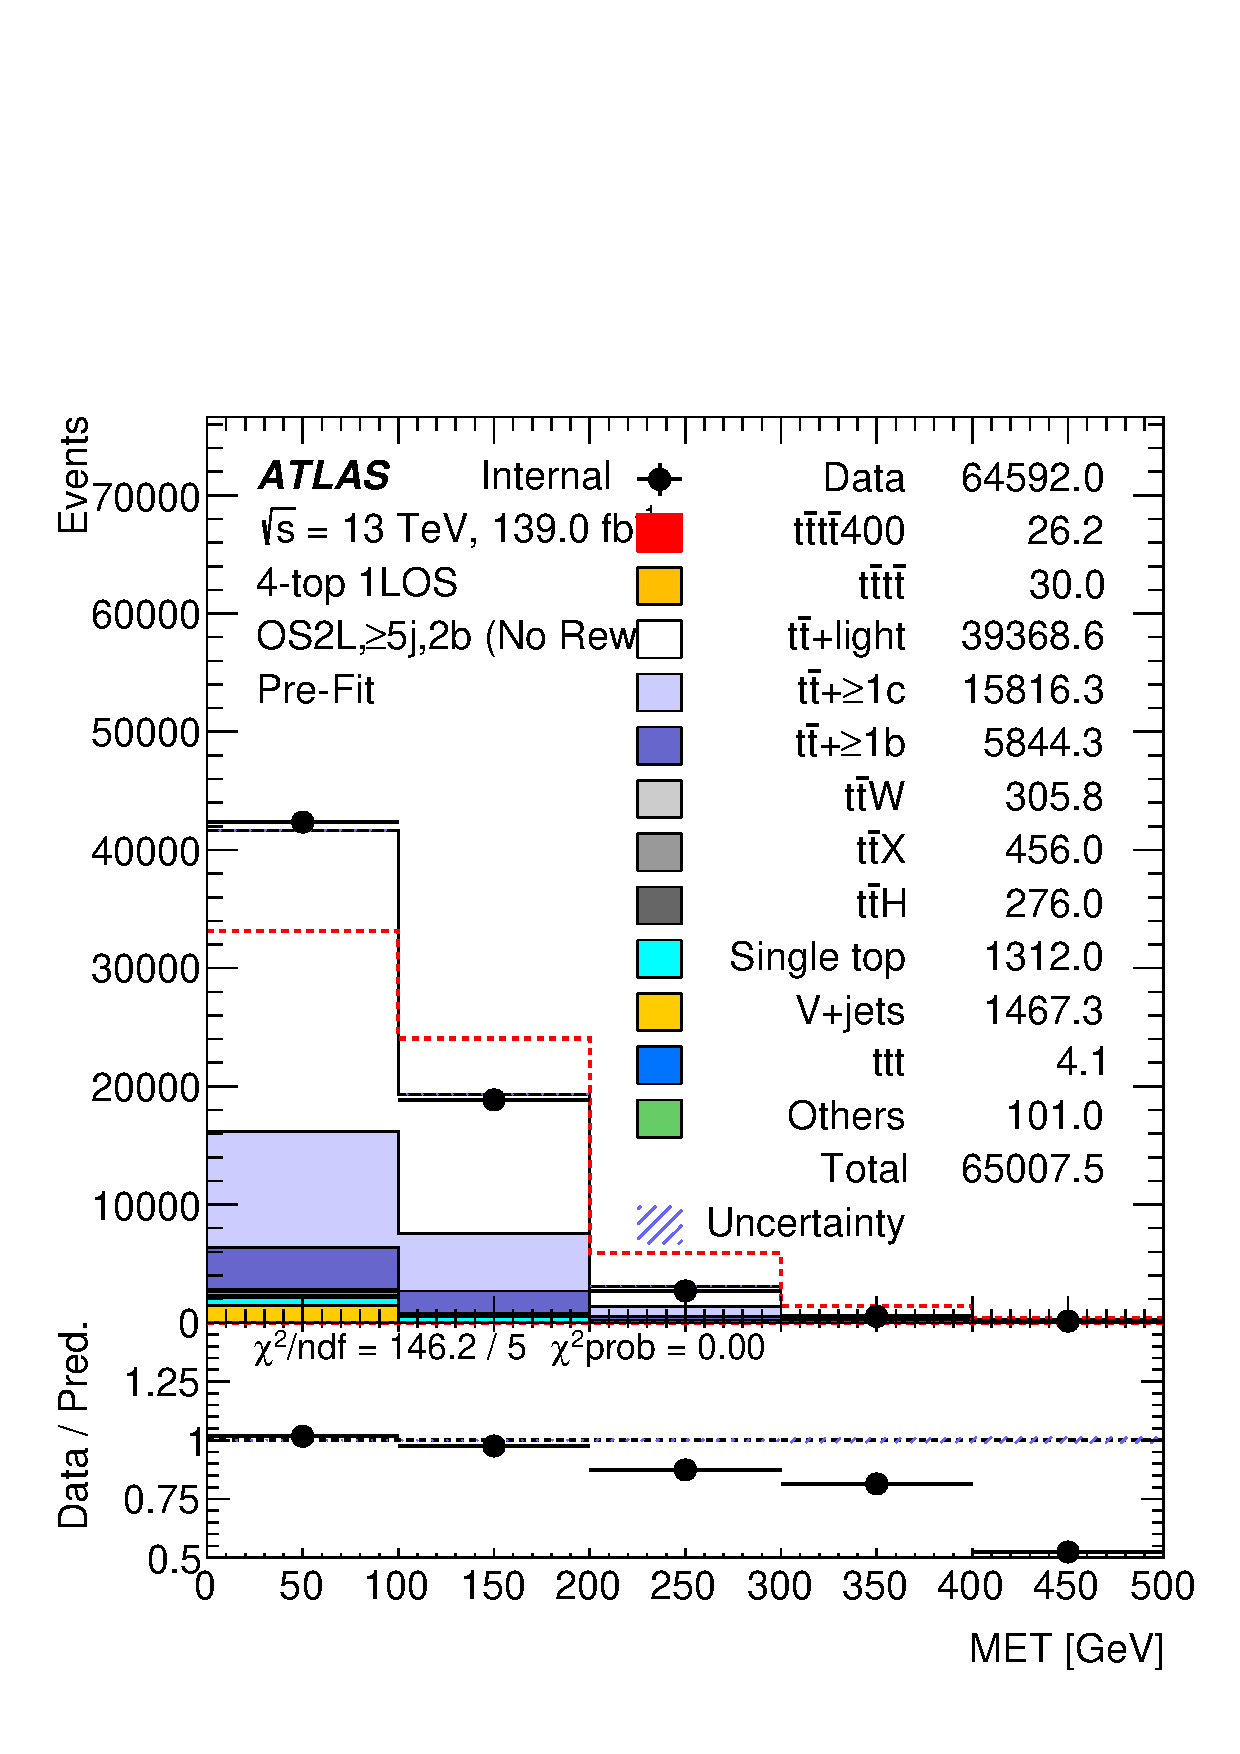
\includegraphics[width=0.4\textwidth]{figures/NNPlots/NNTrainRegion/NoRew/os2l_ge5j2b_met.pdf}
    
\includegraphics[width=0.4\textwidth]{figures/NNPlots/NNTrainRegion/Rew/os2l_ge5j2b_met.pdf}
    \caption{MET}
    \end{center}
    \end{subfigure}

    \begin{subfigure}[t]{1\textwidth}
    \begin{center}
    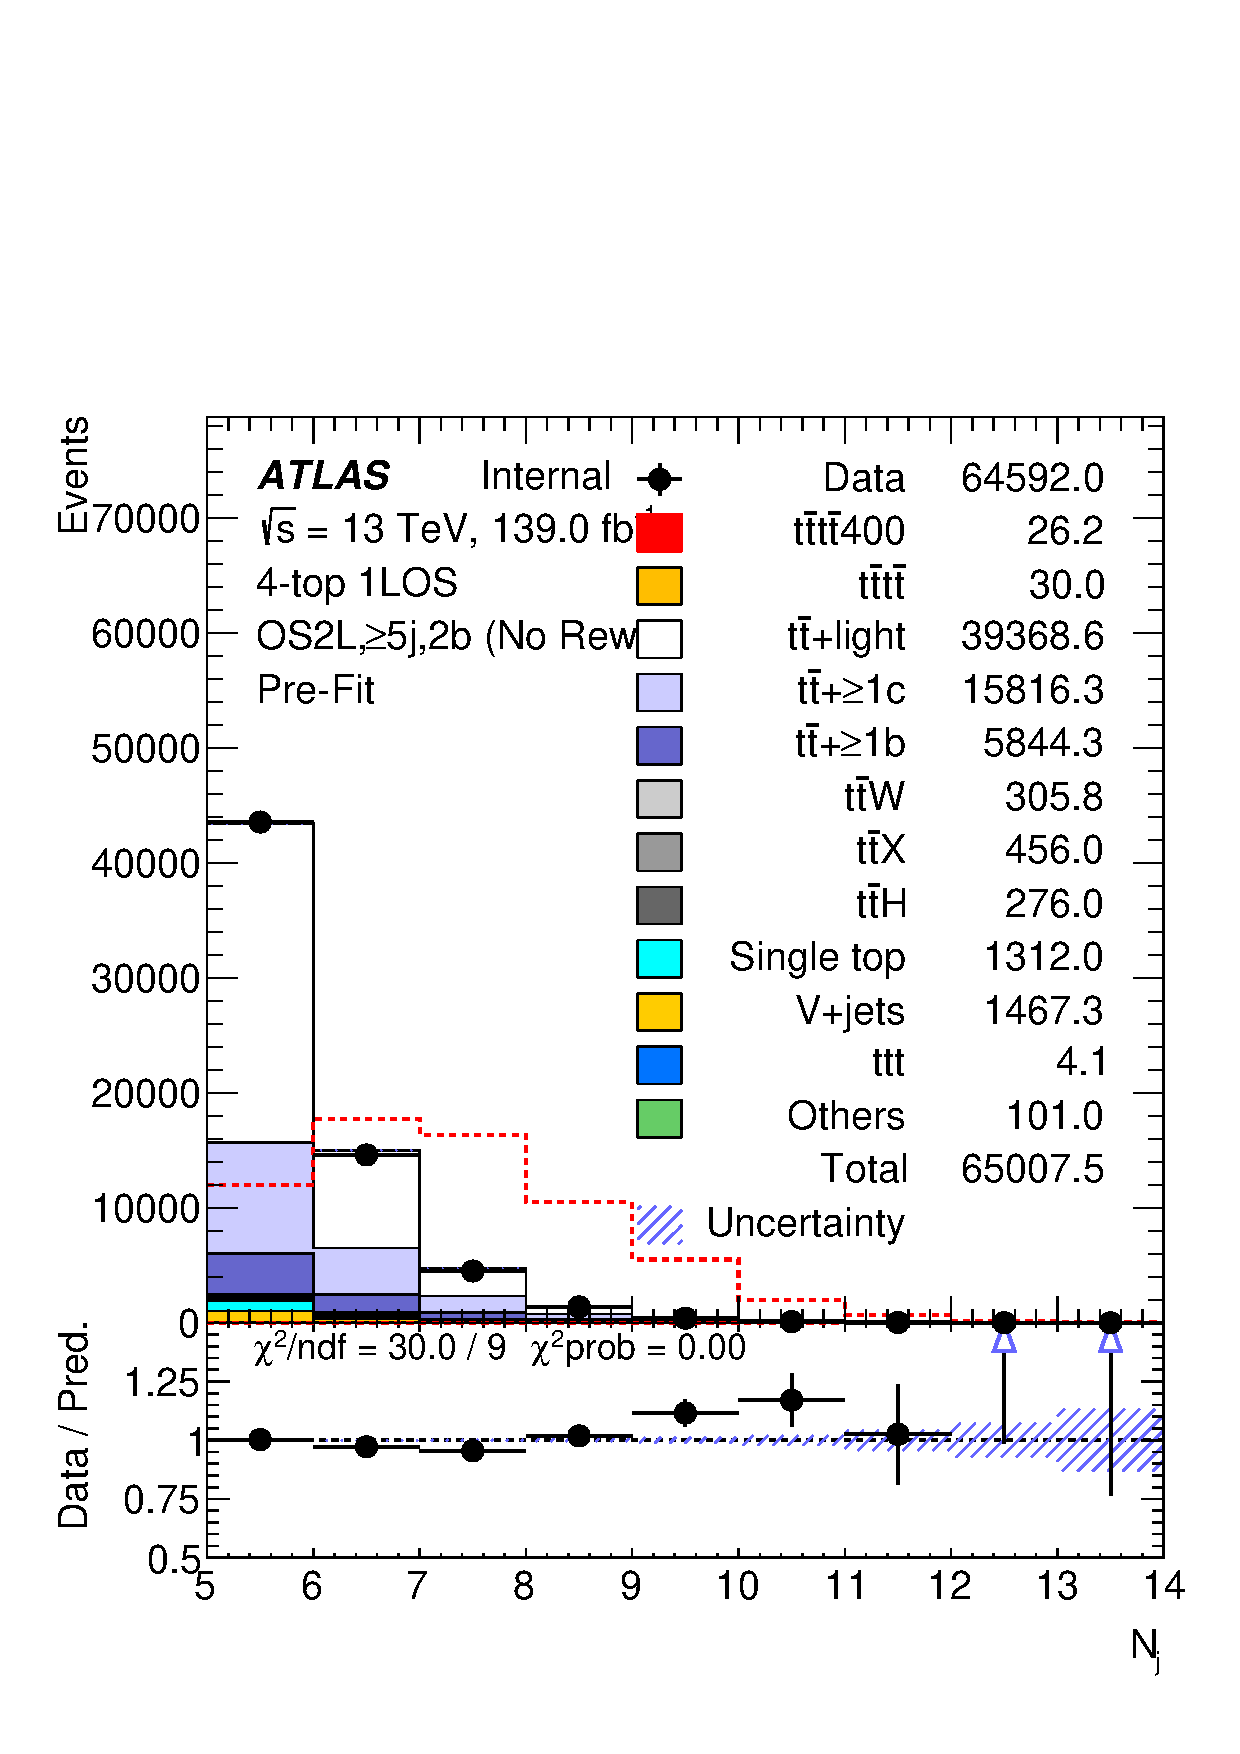
\includegraphics[width=0.4\textwidth]{figures/NNPlots/NNTrainRegion/NoRew/os2l_ge5j2b_nJets.pdf}
    
\includegraphics[width=0.4\textwidth]{figures/NNPlots/NNTrainRegion/Rew/os2l_ge5j2b_nJets.pdf}
    \caption{nJets}
    \end{center}
    \end{subfigure}
    \caption{\label{fig:NNPlots_NNTrainReg_7} The comparison between variables distribution before (left) and after (right) the NN-reweighting in 1L NN training regions ($\geq 5j,=2b$). Blinded regions are excluded.}
\end{figure}

\begin{figure}[htbp!]
    \begin{subfigure}[t]{1\textwidth}
    \begin{center}
    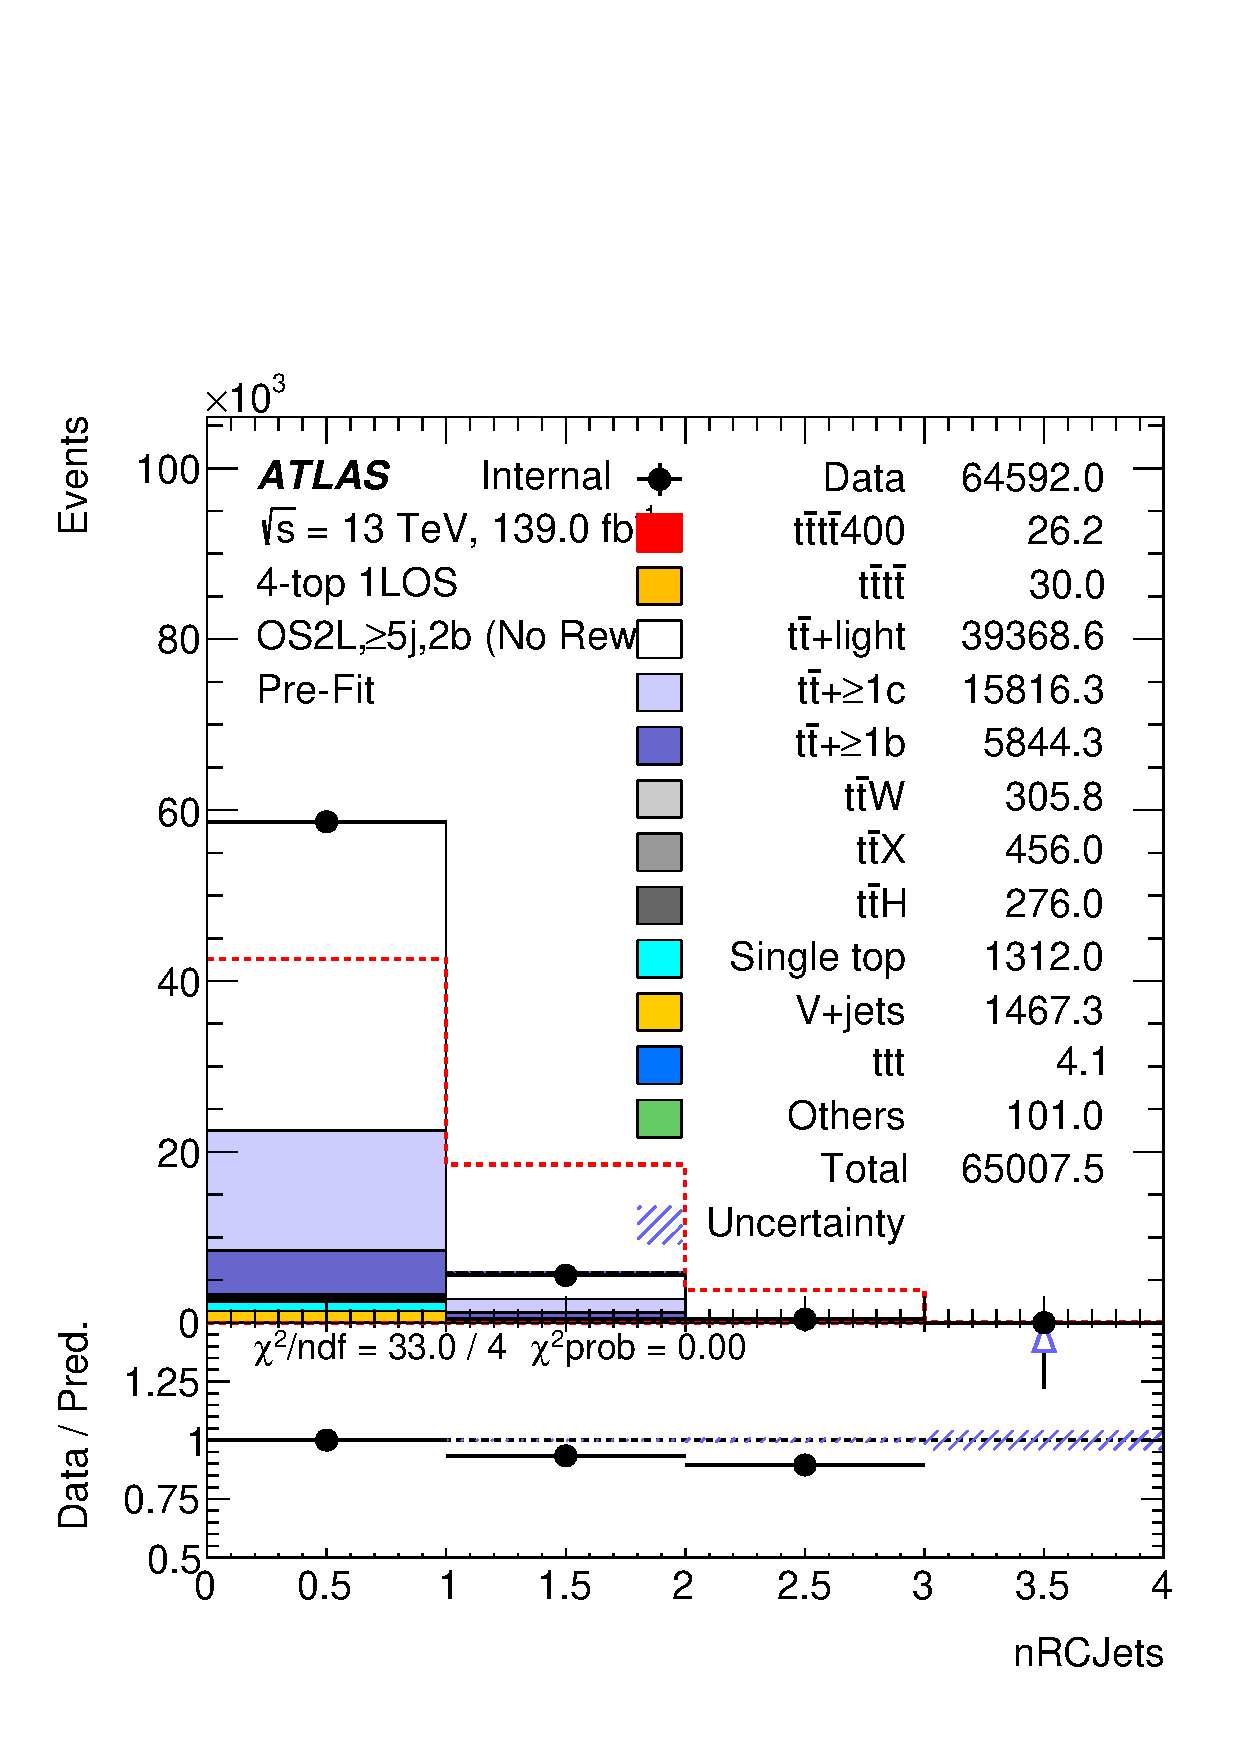
\includegraphics[width=0.4\textwidth]{figures/NNPlots/NNTrainRegion/NoRew/os2l_ge5j2b_nRCJetsM100.pdf}
    
\includegraphics[width=0.4\textwidth]{figures/NNPlots/NNTrainRegion/Rew/os2l_ge5j2b_nRCJetsM100.pdf}
    \caption{nRCJets}
    \end{center}
    \end{subfigure}

    \begin{subfigure}[t]{1\textwidth}
    \begin{center}
    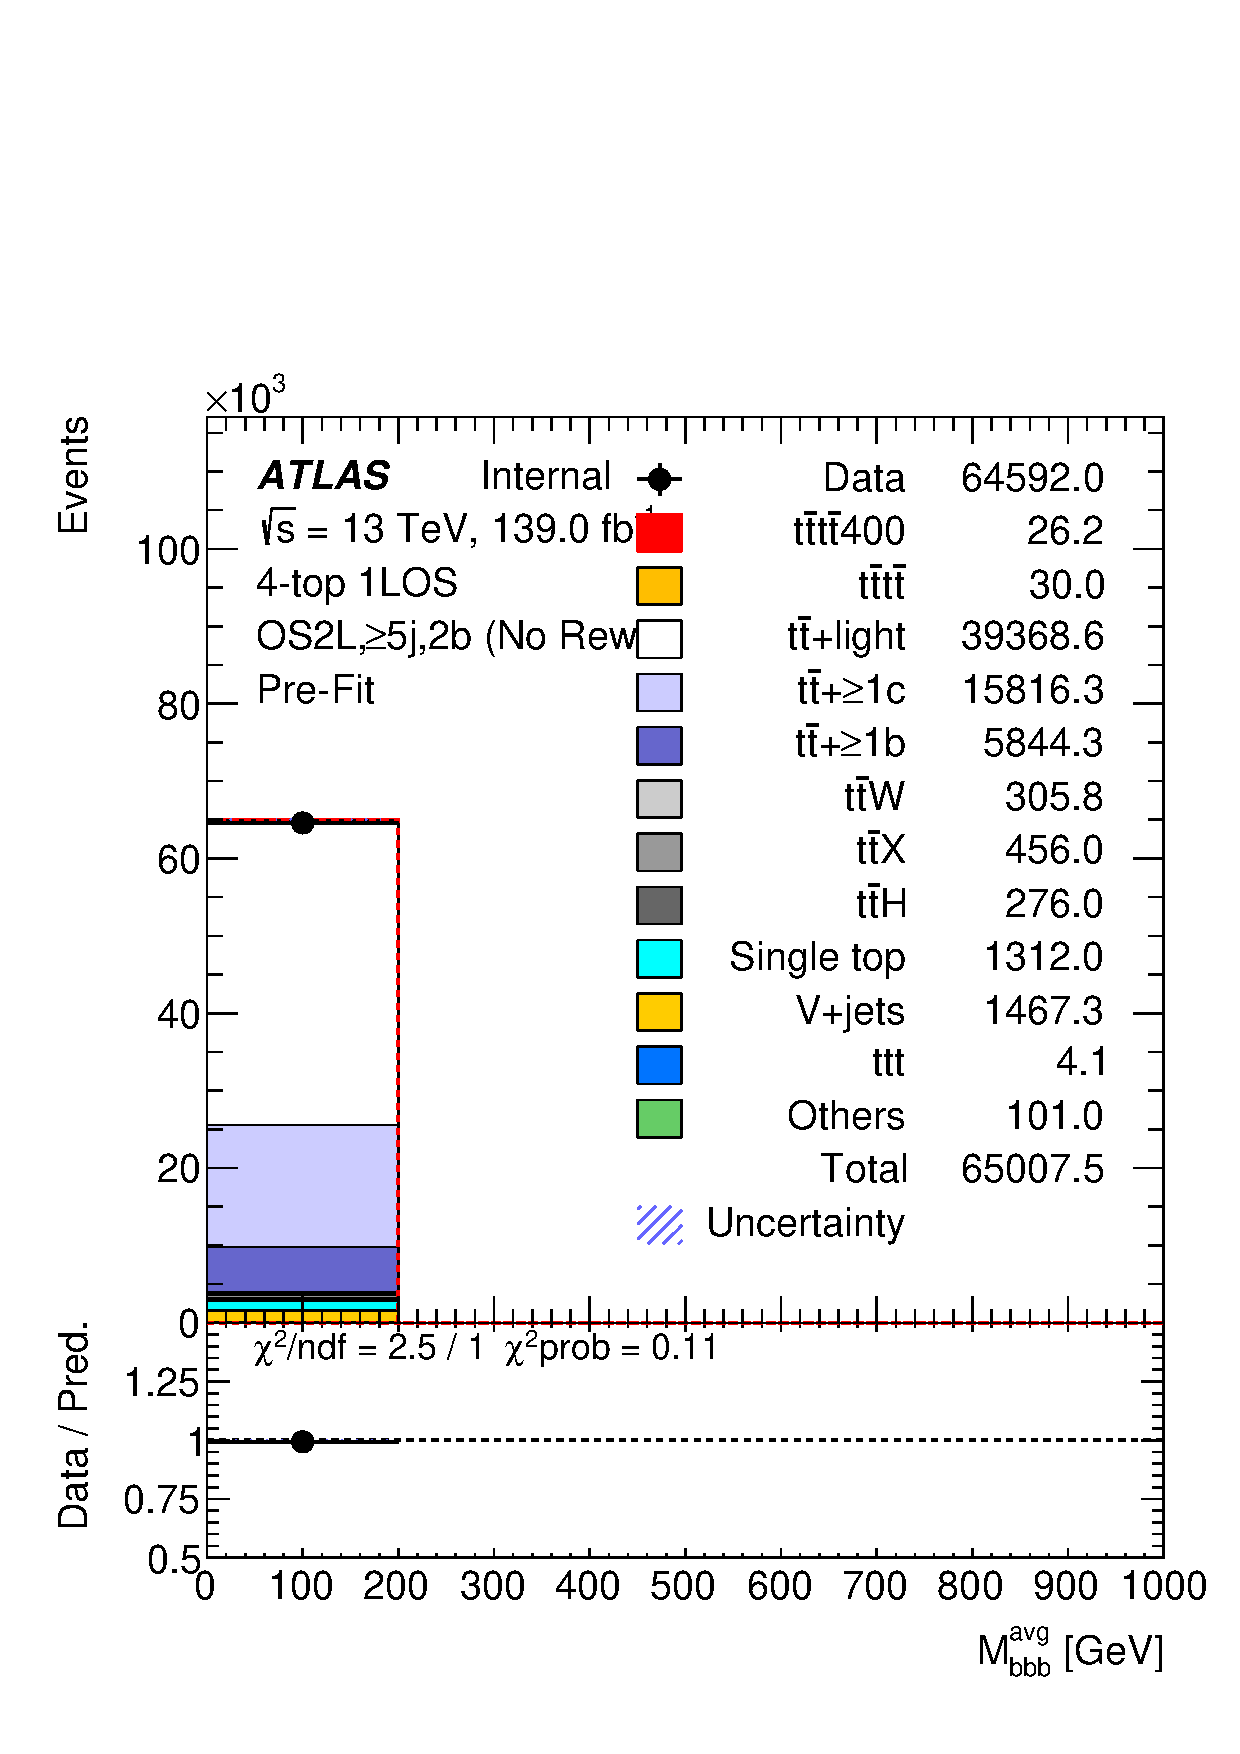
\includegraphics[width=0.4\textwidth]{figures/NNPlots/NNTrainRegion/NoRew/os2l_ge5j2b_Mbbb_Avg_DL1r_70.pdf}
    
\includegraphics[width=0.4\textwidth]{figures/NNPlots/NNTrainRegion/Rew/os2l_ge5j2b_Mbbb_Avg_DL1r_70.pdf}
    \caption{$M^{avg}_{bbb}$}
    \end{center}
    \end{subfigure}

    \begin{subfigure}[t]{1\textwidth}
    \begin{center}
    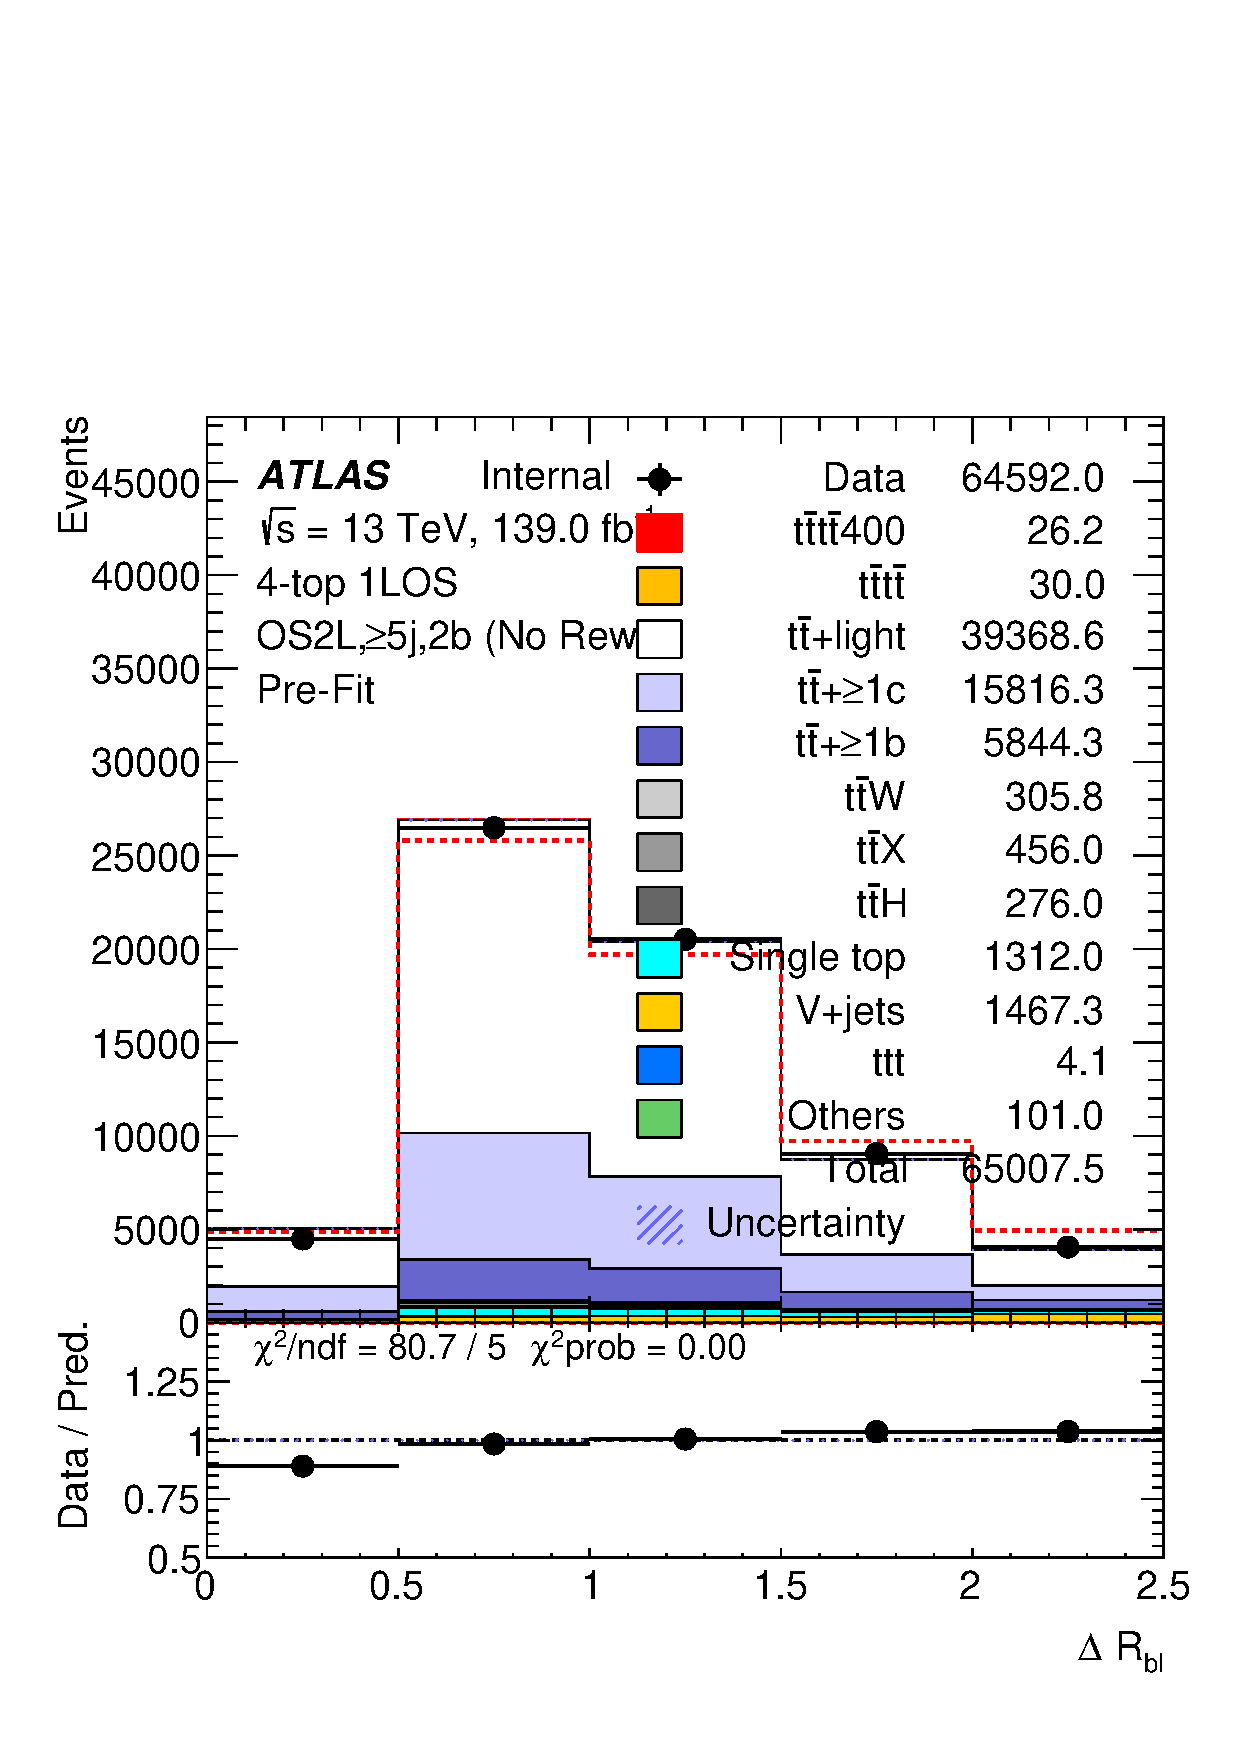
\includegraphics[width=0.4\textwidth]{figures/NNPlots/NNTrainRegion/NoRew/os2l_ge5j2b_dRbl_MindR_DL1r_70.pdf}
    
\includegraphics[width=0.4\textwidth]{figures/NNPlots/NNTrainRegion/Rew/os2l_ge5j2b_dRbl_MindR_DL1r_70.pdf}
    \caption{$\Delta R^{min}_{bl}$}
    \end{center}
    \end{subfigure}
    \caption{\label{fig:NNPlots_NNTrainReg_8} The comparison between variables distribution before (left) and after (right) the NN-reweighting in 1L NN training regions ($\geq 5j,=2b$). Blinded regions are excluded.}
\end{figure}

\begin{figure}[htbp!]
    \begin{subfigure}[t]{1\textwidth}
    \begin{center}
    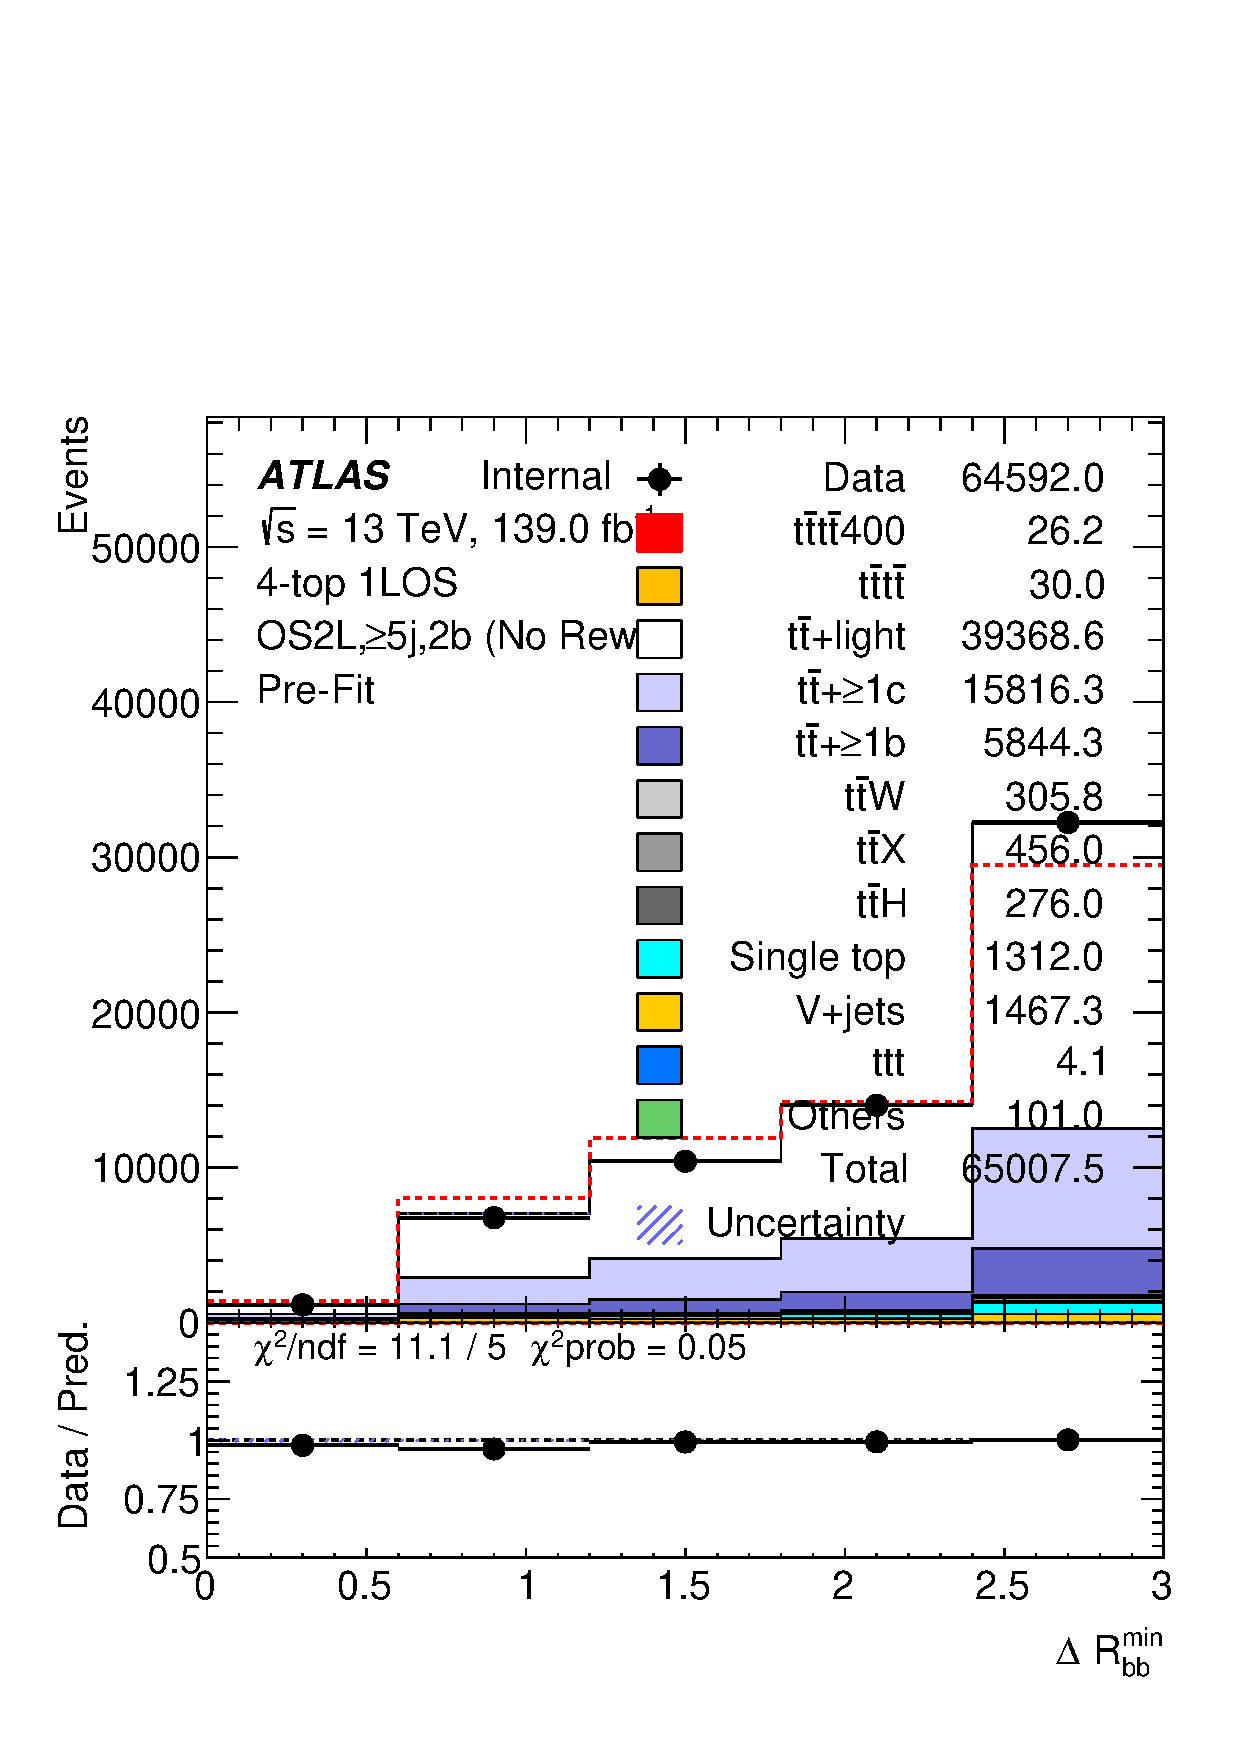
\includegraphics[width=0.4\textwidth]{figures/NNPlots/NNTrainRegion/NoRew/os2l_ge5j2b_dRbb_MindR_DL1r_70.pdf}
    
\includegraphics[width=0.4\textwidth]{figures/NNPlots/NNTrainRegion/Rew/os2l_ge5j2b_dRbb_MindR_DL1r_70.pdf}
    \caption{$\Delta R^{min}_{bb}$}
    \end{center}
    \end{subfigure}

    \begin{subfigure}[t]{1\textwidth}
    \begin{center}
    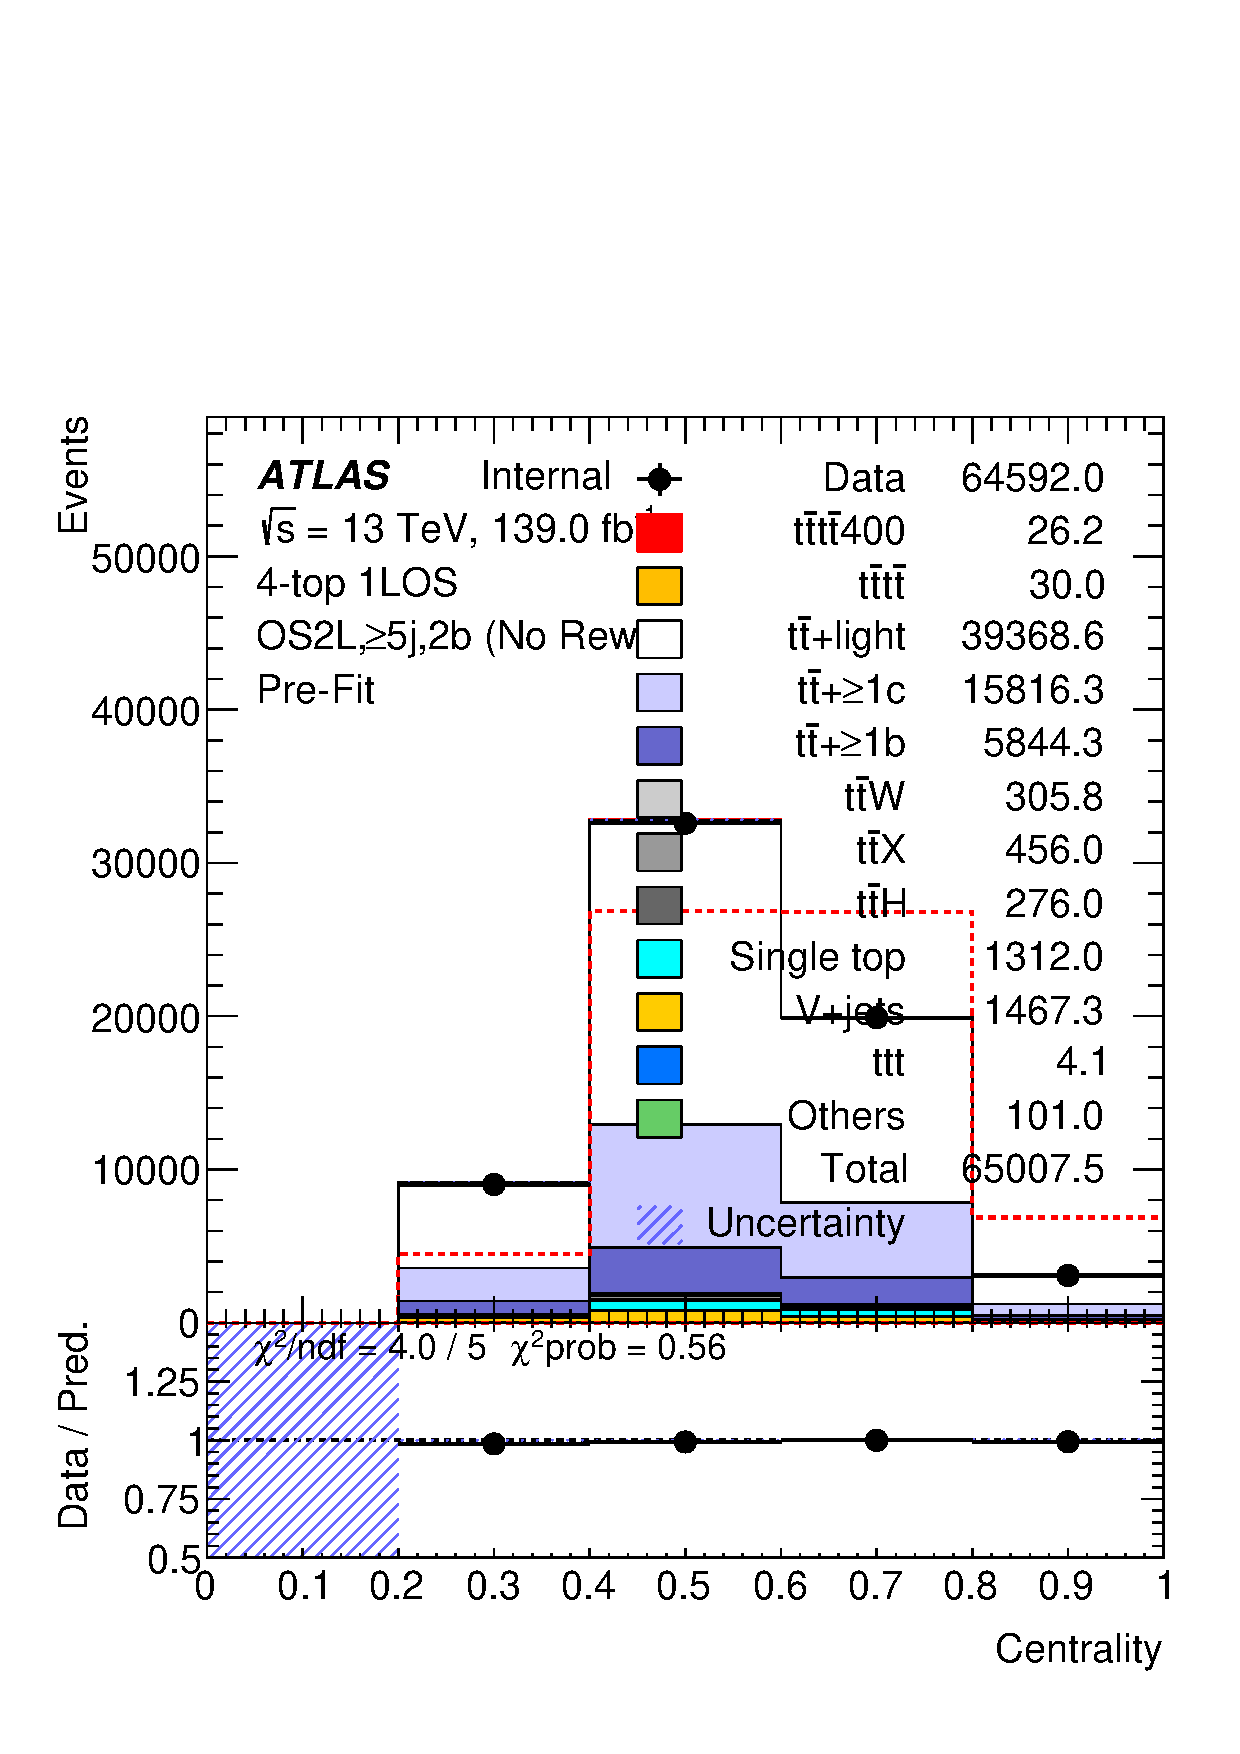
\includegraphics[width=0.4\textwidth]{figures/NNPlots/NNTrainRegion/NoRew/os2l_ge5j2b_Centrality_all.pdf}
    
\includegraphics[width=0.4\textwidth]{figures/NNPlots/NNTrainRegion/Rew/os2l_ge5j2b_Centrality_all.pdf}
    \caption{Centrality}
    \end{center}
    \end{subfigure}

    \begin{subfigure}[t]{1\textwidth}
    \begin{center}
    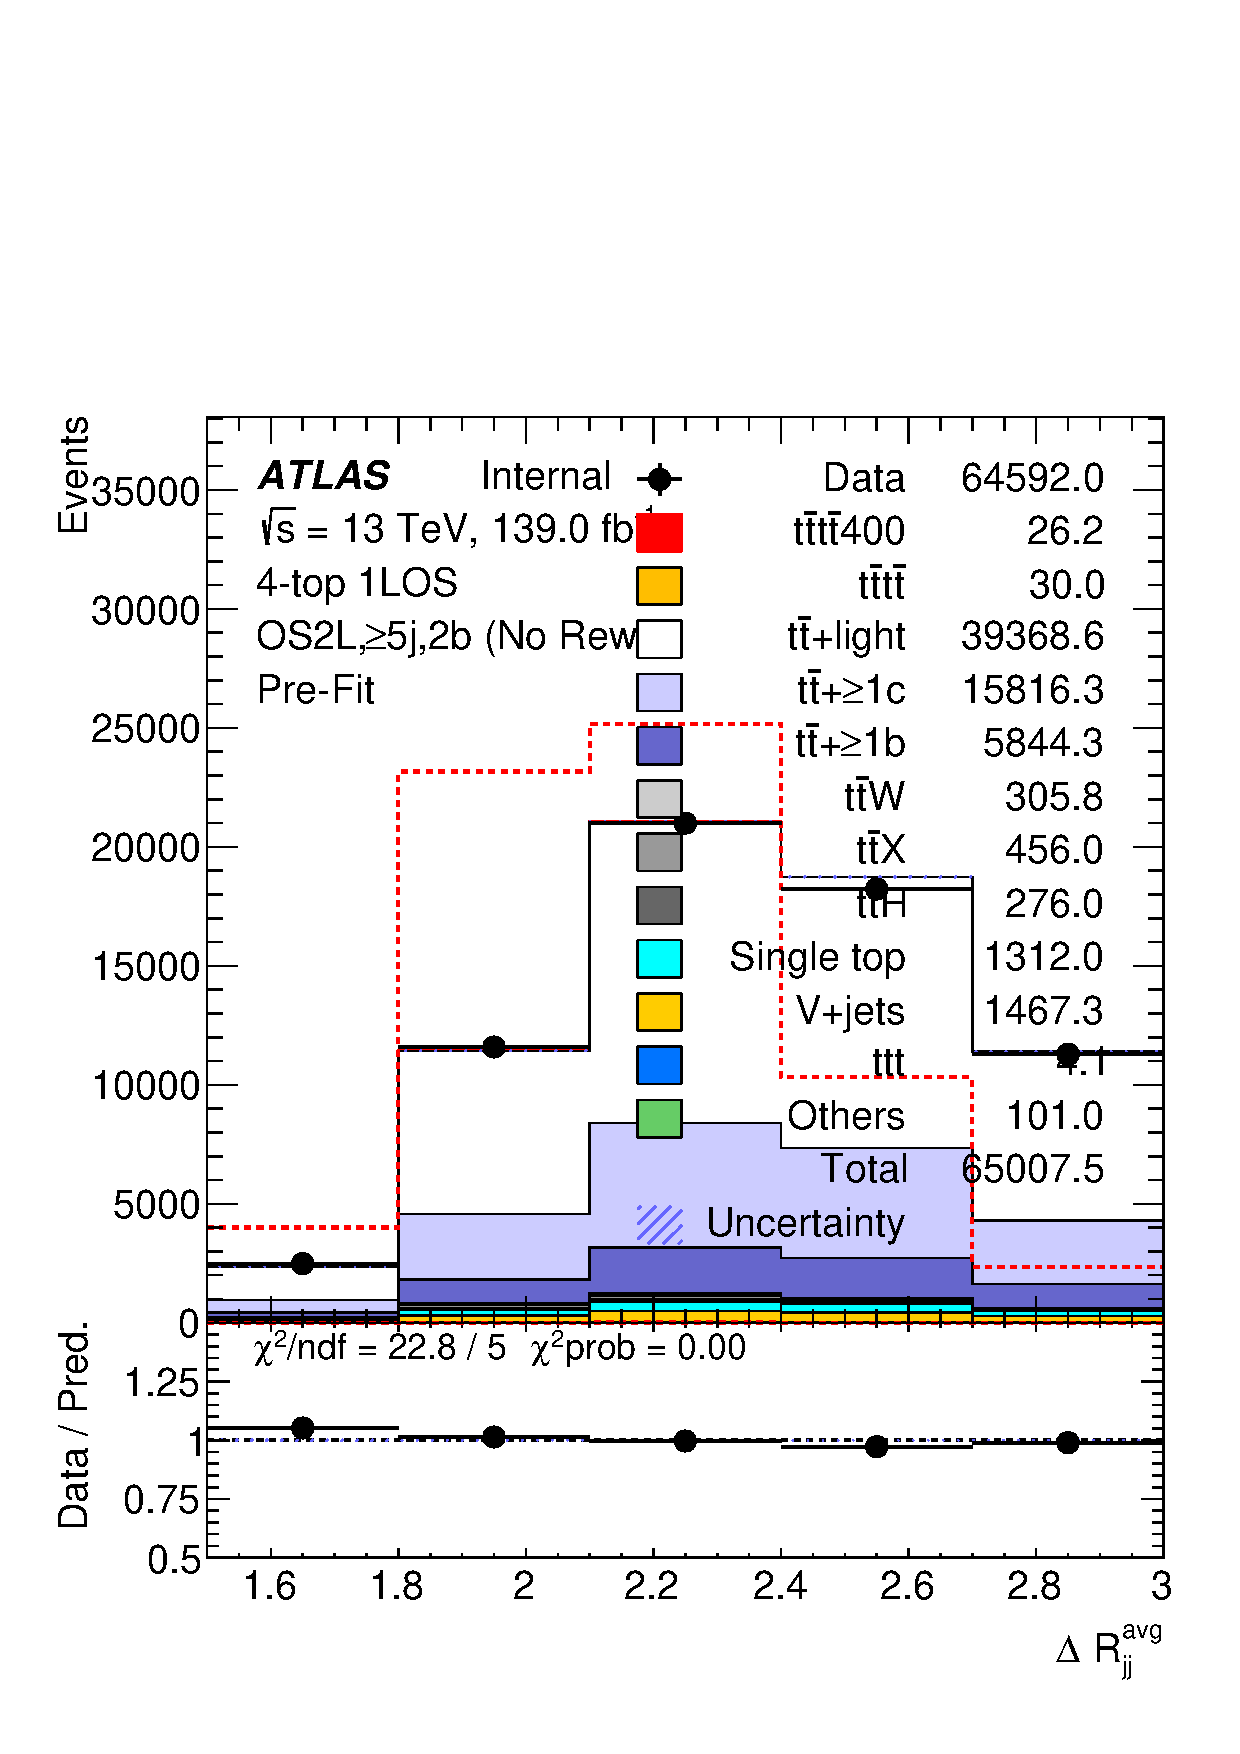
\includegraphics[width=0.4\textwidth]{figures/NNPlots/NNTrainRegion/NoRew/os2l_ge5j2b_dRjj_Avg.pdf}
    
\includegraphics[width=0.4\textwidth]{figures/NNPlots/NNTrainRegion/Rew/os2l_ge5j2b_dRjj_Avg.pdf}
    \caption{$\Delta R^{avg}_{jj}$}
    \end{center}
    \end{subfigure}
    \caption{\label{fig:NNPlots_NNTrainReg_9} The comparison between variables distribution before (left) and after (right) the NN-reweighting in 1L NN training regions ($\geq 5j,=2b$). Blinded regions are excluded.}
\end{figure}

\begin{figure}[htbp!]
    \begin{subfigure}[t]{1\textwidth}
    \begin{center}
    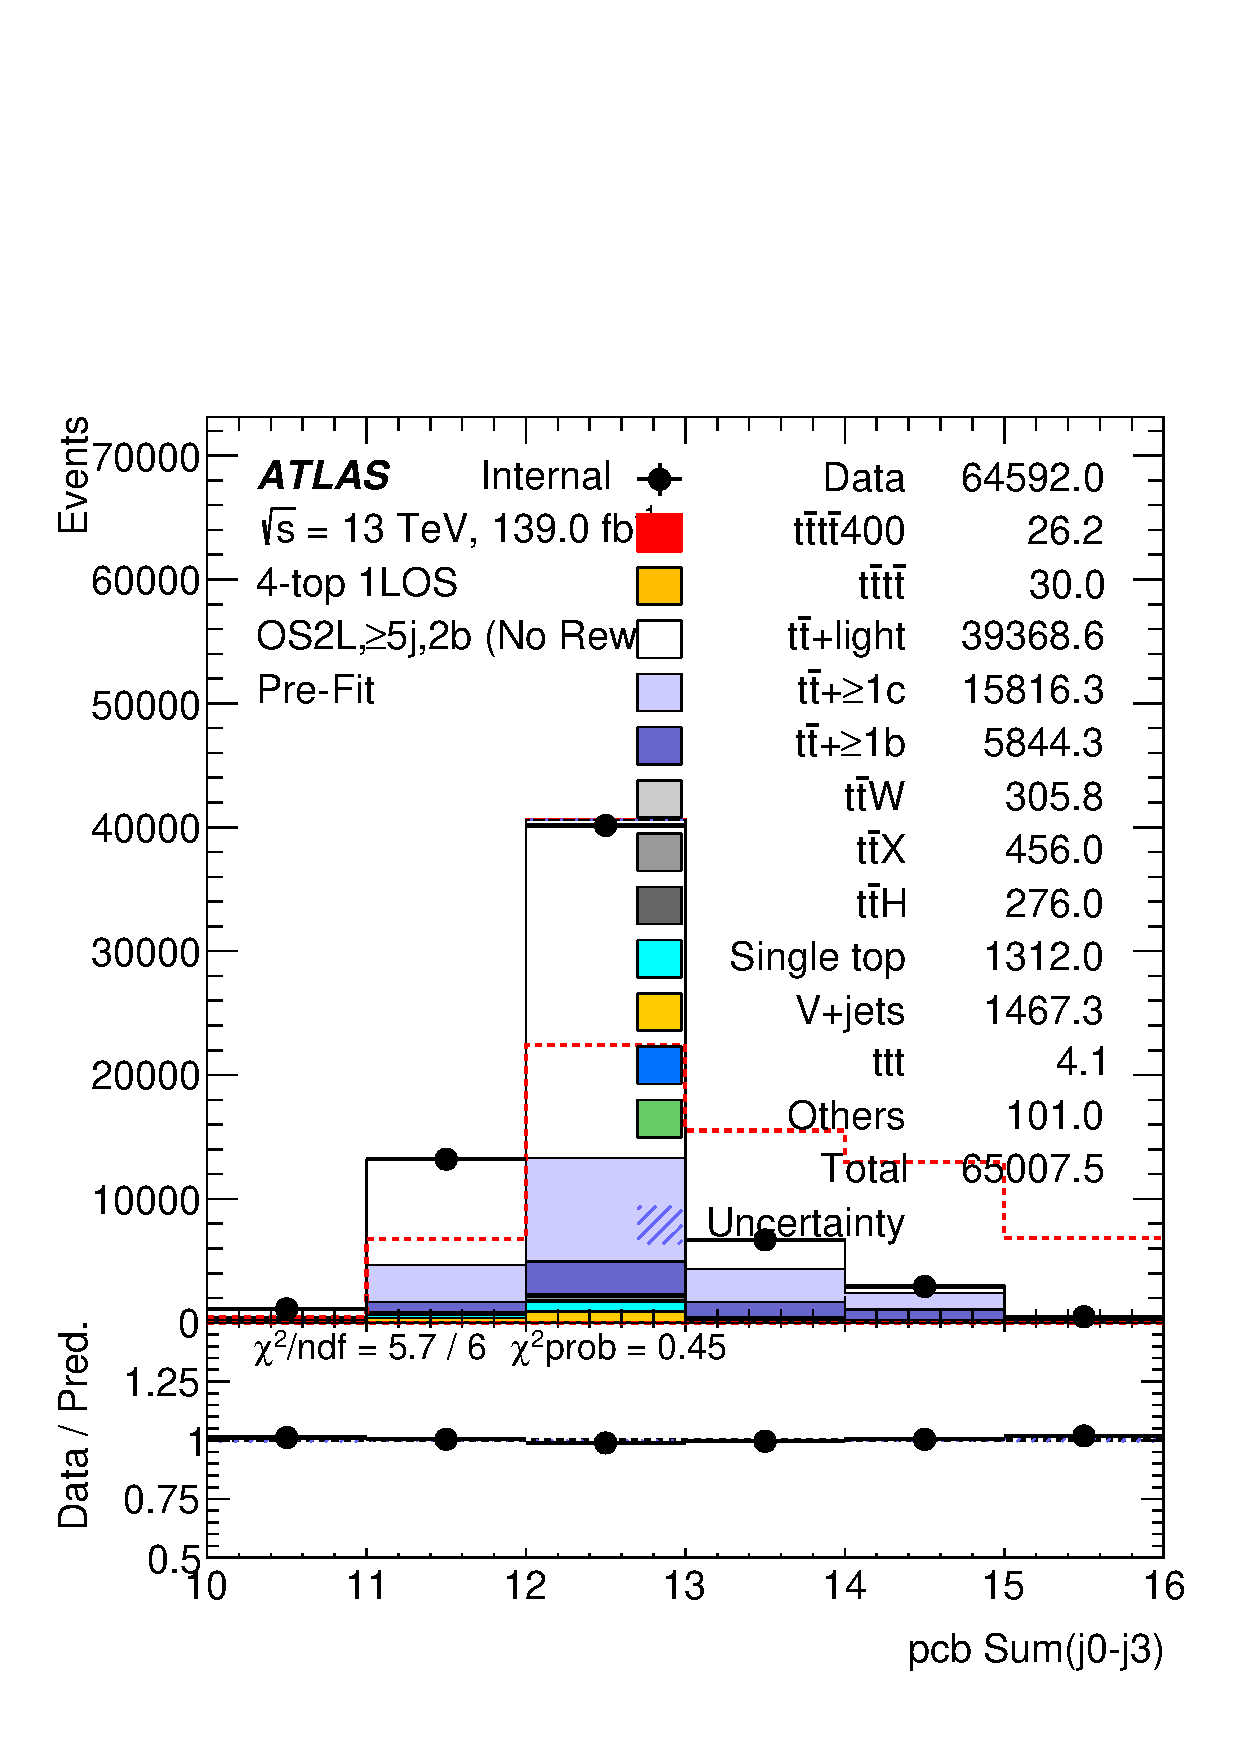
\includegraphics[width=0.4\textwidth]{figures/NNPlots/NNTrainRegion/NoRew/os2l_ge5j2b_pcb.pdf}
    
\includegraphics[width=0.4\textwidth]{figures/NNPlots/NNTrainRegion/Rew/os2l_ge5j2b_pcb.pdf}
    \caption{pcb Sum}
    \end{center}
    \end{subfigure}

    \begin{subfigure}[t]{1\textwidth}
    \begin{center}
    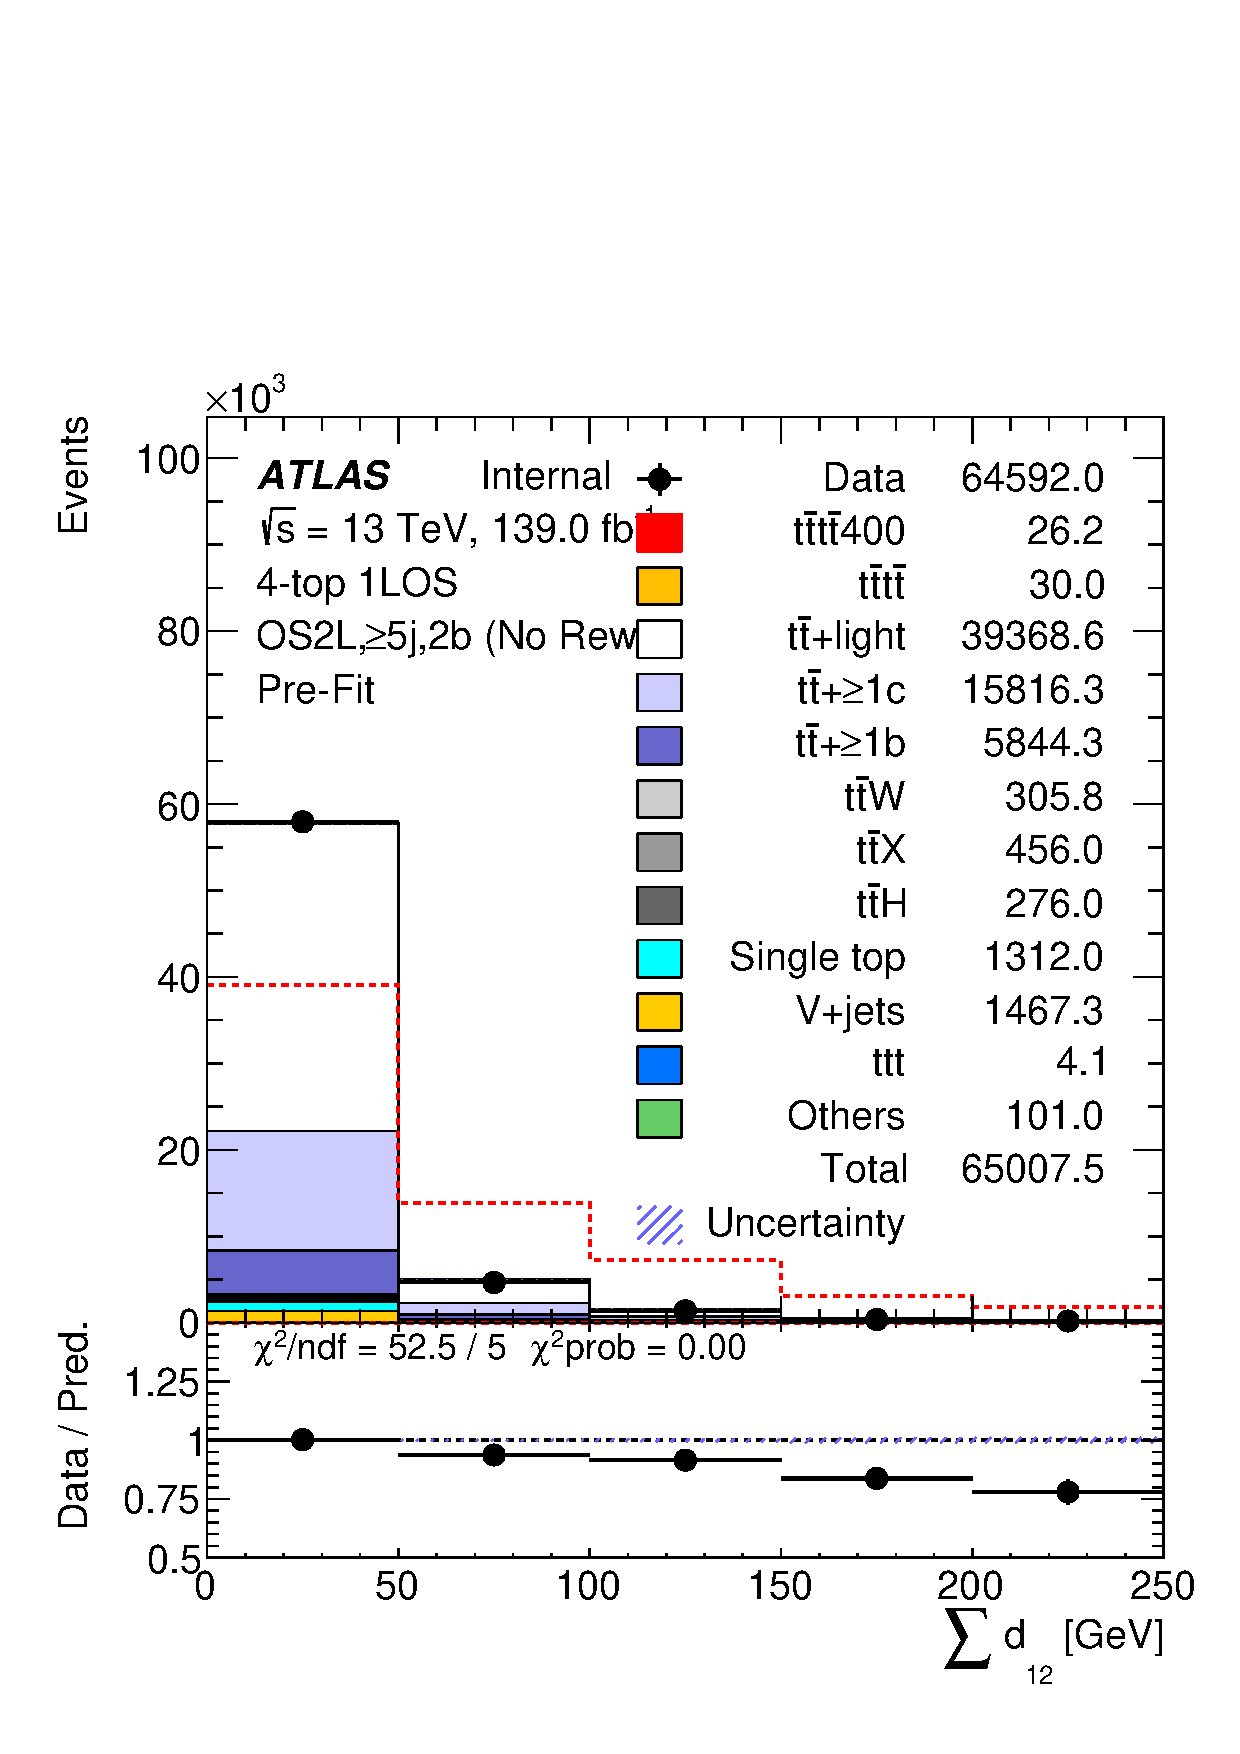
\includegraphics[width=0.4\textwidth]{figures/NNPlots/NNTrainRegion/NoRew/os2l_ge5j2b_sum_d12.pdf}
    
\includegraphics[width=0.4\textwidth]{figures/NNPlots/NNTrainRegion/Rew/os2l_ge5j2b_sum_d12.pdf}
    \caption{$\sum d_{12}$}
    \end{center}
    \end{subfigure}

    \begin{subfigure}[t]{1\textwidth}
    \begin{center}
    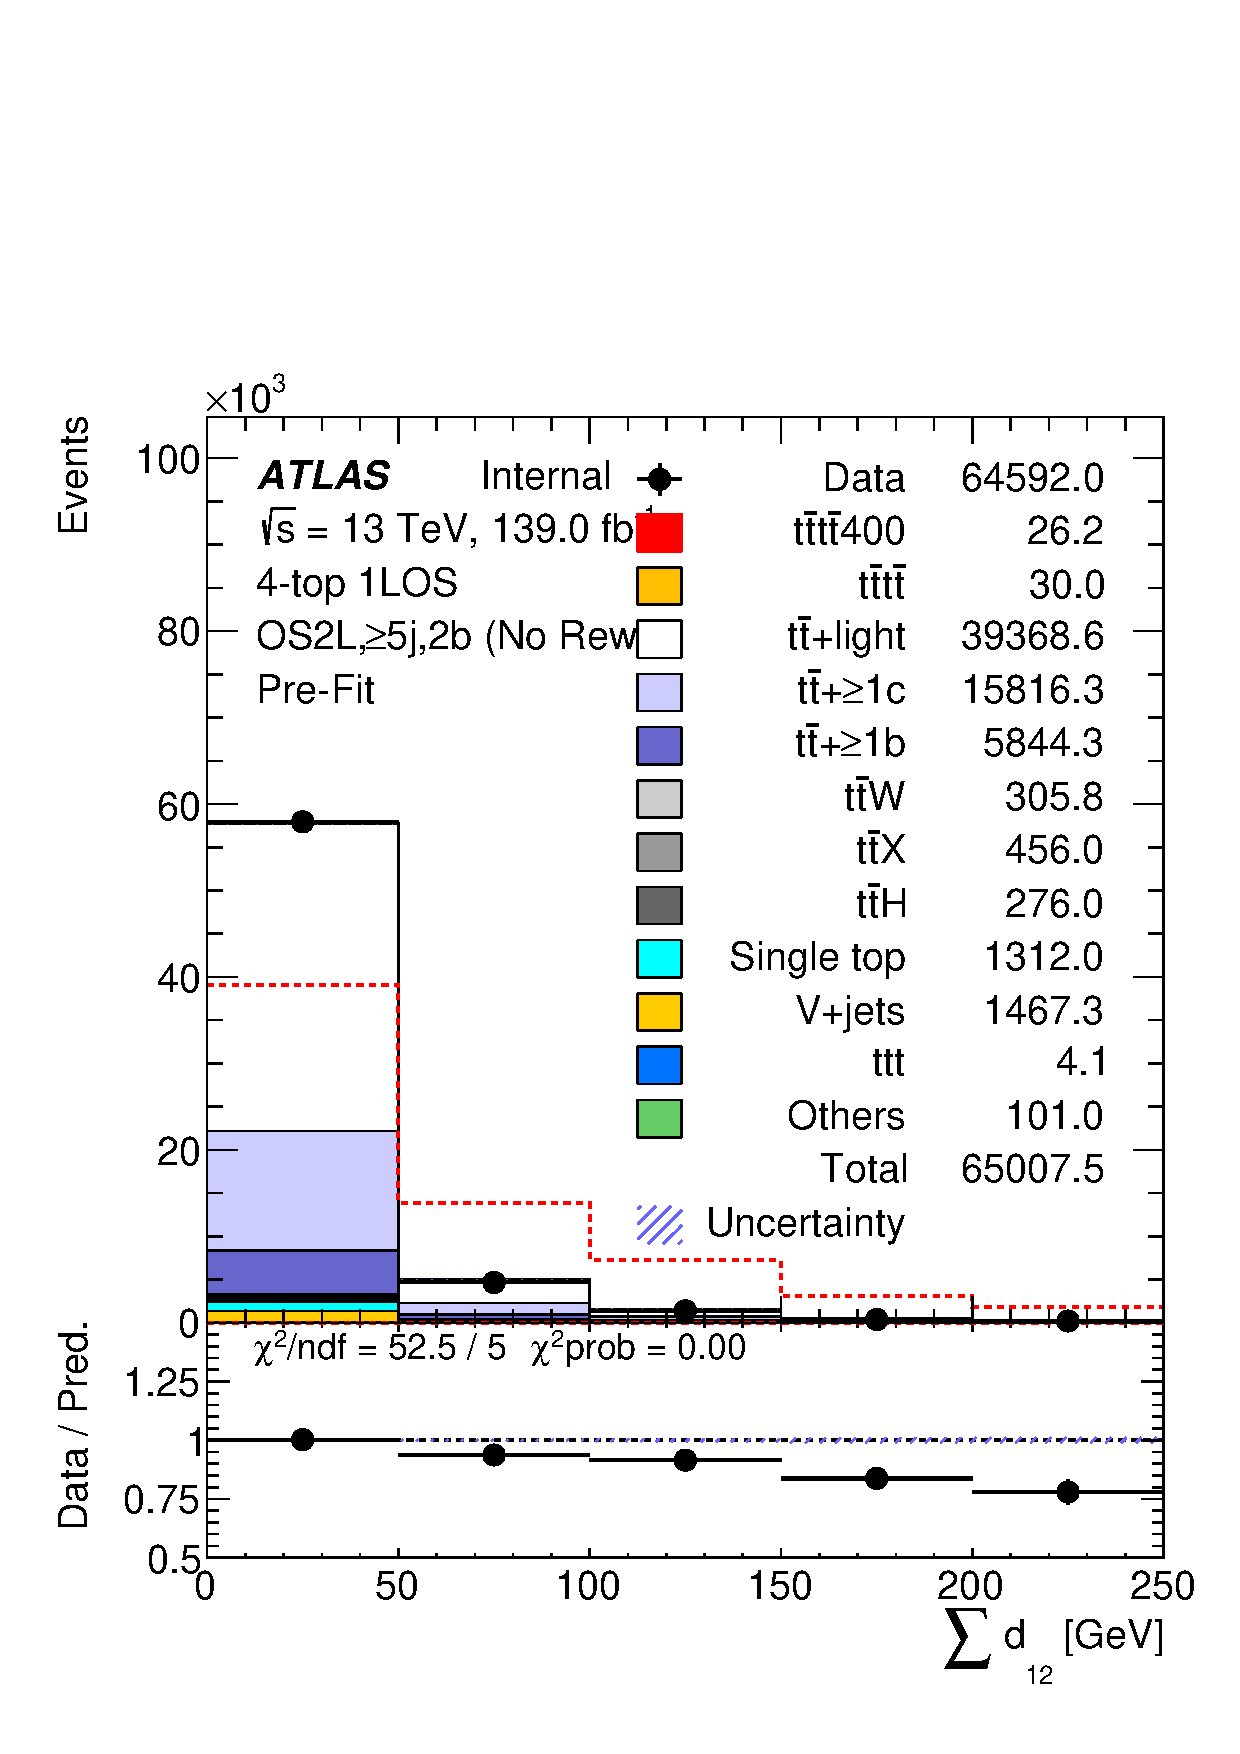
\includegraphics[width=0.4\textwidth]{figures/NNPlots/NNTrainRegion/NoRew/os2l_ge5j2b_sum_d23.pdf}
    
\includegraphics[width=0.4\textwidth]{figures/NNPlots/NNTrainRegion/Rew/os2l_ge5j2b_sum_d23.pdf}
    \caption{$\sum d_{23}$}
    \end{center}
    \end{subfigure}
    \caption{\label{fig:NNPlots_NNTrainReg_10} The comparison between variables distribution before (left) and after (right) the NN-reweighting in 1L NN training regions ($\geq 5j,=2b$). Blinded regions are excluded.}
\end{figure}